\documentclass[english]{report}
\usepackage[utf8]{inputenc}
%\usepackage[UKenglish]{duomasterforside}
%\usepackage{siunitx}
\RequirePackage[a4paper]{geometry}
\geometry{twoside,vmargin=4.5cm,inner=4cm,outer=3cm}

%\documentclass[reprint, nofootinbib]{revtex4-1}
%\usepackage{scrextend}
%% Mathematics
\usepackage{amssymb}   % Extra symbols
\usepackage{amsthm}    % Theorem-like environments
\usepackage{thmtools}  % Theorem-like environments
\usepackage{mathtools} % Fonts and environments for mathematical formuale
\usepackage{mathrsfs}  % Script font with \mathscr{}
\usepackage{bm}

% For breaking url's at - too, not only \
\usepackage{url}
\def\UrlBreaks{\do\/\do-}



\usepackage{unicode-math}
%\setmathfont{XITSMath-Regular.otf}
%\usepackage[bottom]{footmisc}
%% Miscellanous
\usepackage{graphicx}  % Tool for images
\usepackage{siunitx}
\usepackage{hyperref}
\graphicspath{{figures/}}
\usepackage[english]{babel}     % Automatic translations
\usepackage{csquotes}  % Quotes
\usepackage{textcomp}  % Extra symbols
\usepackage{listings}  % Typesetting code
%\lstset{basicstyle = \ttfamily, frame = tb}
%\usepackage{fancyhdr}
%\pagestyle{fancy}
%\renewcommand{\footrulewidth}{0.4pt}% default is 0pt
%\usepackage{subfig}
\usepackage{setspace}
\usepackage{comment}
\usepackage{braket}

%\documentclass[a4paper,12pt,twoside]{book}
%\usepackage[utf8]{inputenc}
%\usepackage[english]{babel}
%\usepackage{fancyhdr}

% Use more than one option in new command
\usepackage{xargs} 

\usepackage{multirow}
\usepackage{booktabs}
\usepackage{cite}
% To write fancy notes in PDF
\usepackage{todonotes}

%Customized comments for the todonotes package
% Normal use (add inline to usen in line and in figures etc: \todo[inline]{The original todo note withouth changed colours.} 
\newcommandx{\improvement}[2][1=]{\todo[linecolor=red,backgroundcolor=red!25,bordercolor=red,#1]{#2}}
\newcommandx{\change}[2][1=]{\todo[linecolor=blue,backgroundcolor=blue!25,bordercolor=blue,#1]{#2}}
\newcommandx{\info}[2][1=]{\todo[linecolor=OliveGreen,backgroundcolor=OliveGreen!25,bordercolor=OliveGreen,#1]{#2}}
\newcommandx{\unsure}[2][1=]{\todo[linecolor=Plum,backgroundcolor=Plum!25,bordercolor=Plum,#1]{#2}}

%\renewcommand{\footrulewidth}{0.4pt}% default is 0pt

%\pagestyle{fancy}
%\fancyhf{}
%\fancyhead[LE,RO]{Master thesis}
%\fancyhead[RE,LO]{Mona Anderssen}
%\fancyfoot[CE,CO]{\leftmark}
%\fancyfoot[LE,RO]{\thepage}
%\lstset{basicstyle = \ttfamily, frame = tb}
%\setcounter{secnumdepth}{8}

\usepackage{graphicx}
\usepackage{float}
\usepackage{caption}
\usepackage{subcaption}
\usepackage{babel, duomasterforside}
%\usepackage{subfig}
%\usepackage{hyperref}

%\usepackage{lipsum}
\usepackage{mathrsfs}
\pagenumbering{roman}

\renewcommand{\chaptername}{}

\title{Performance of deep learning in searches for new physics phenomena in events with leptons and missing transverse energy with the ATLAS detector at the LHC}
\author{Mona Anderssen}

\setlength{\parindent}{0em}
\setlength{\parskip}{1em}
\renewcommand{\baselinestretch}{1.5}
%\baselinestretch
\begin{document}
{\setstretch{1.0}
\duoforside[dept = {Department of Physics}, program = {Nuclear and particle physics}]
}

%\begin{titlepage}
   \begin{center}
       \vspace*{1cm}
 
       \LARGE{\textbf{Performance of deep learning in searches for new physics phenomena in events with leptons and missing transverse energy with the ATLAS detector at the LHC}}
 
       \vspace{0.5cm}
 
       \vspace{1.5cm}
 
       \large{\textbf{Mona Anderssen}}
 
       \vfill
 
       Thesis submitted for the degree of Master in particle and nuclear physics\\
       60 credits\\
 
       \vspace{0.8cm}
 
       
\includegraphics[width=0.4\textwidth]{Figures/UiO_Segl_pms485.eps}
 
       Department of Physics\\
       Faculty of mathematics and natural sciences\\
       UNIVERSITY OF OSLO\\
       Fall 2020
 
   \end{center}
\end{titlepage}
\begin{abstract}
    In this thesis we have been searching for new physics phenomena using ML methods, such as BDTs and NNs. The data used for training and testing the ML methods were collected by the ATLAS experiment at the LHC, and were collected in the period 2015-2018. The ML methods was trained on different compositions of mass splittings and features, and have overall performed very well. Both ML methods have been compared to results done with the more traditional method, cut and count, and ML seems to be more sensitive for the signals we have used. 
\end{abstract}
\tableofcontents
\listoftables
\listoffigures
\pagenumbering{arabic}
%\addcontentsline{toc}{chapter}{Introduction}
\chapter*{Introduction}
\label{sec:Introduction}
The Standard Model (SM) \cite{thomson} is a well known theory of particle physics lately further confirmed after the Higgs boson was discovered at CERN in 2012 by the ATLAS \cite{Higgs_ATLAS} and CMS \cite{Higgs_CMS} collaborations. The SM can describe all visible matter and contains matter particles, quarks and leptons, and the fundamental forces acting between them. Even though the SM can describe all the matter we can see around us, it can't describe the whole universe. There are of course many theories which attempt to addvers the shortcomings of the SM, but in this thesis we mainly focus on Supersymmetry (SUSY) and non-SUSY Dark Matter (DM) simplified models. SUSY is an extension of the SM which predicts that every particle in the SM has a supersymmetric partner with equal quantum numbers, except for the spin. One of the consequences of discovering SUSY may be that it provides a DM candidate, which we are going to look more into in this thesis.

For many years the standard way to perform an analysis have been to simply apply cuts kinematical variables, which efficiently discriminate new physics signal from SM background. The set of cuts define signal regions, which are optimized to lead to the best sensitivity, i.e. the highest signal over background ratio. However, these methods have limitations when it comes to discovering and using correlations between variables. Cut and count methods usually apply cuts evaluating one variable at the time or use so-called rectangular cuts evaluating the correlation between maximum two variables. With computers and new algorithms constantly being improved and developed, particle physicists have tried to look for other possibilities to perform searches for new physics, namely by using Machine Learning (ML) based methods and algorithms. ML methods, in contrast to the cut and count methods, can investigate multidimensional correlations and place cuts using boundaries in higher dimensions. ML has therefore become very popular and is widely used in many fields of research. In this thesis we explore Boosted Decision Trees (BDTs) and Neural Networks (NNs), and compare the results against each other and with a more traditional cut and count analysis. 

In chapter \ref{sec:Theory} a short introduction to the SM and new physics will be given. Chapter \ref{sec:LHCandATLAS} contains a short presentation of the detector and the computing infrastructure to analyze 13 TeV data collected by the ATLAS experiment at the Large Hadron Collider.. We will then move to the search for new physics with the cut and count method in chapter \ref{sec:CandCanalysis}. The next chapters (\ref{sec:ML} and \ref{sec:MLanalysis}) introduce Machine Learning algorithms and apply them to the searches introduced in chapter \ref{sec:CandCanalysis}. In the end present our results and compare the traditional and ML-based methods in chapter \ref{sec:results} and conclude in chapter \ref{sec:Conclusion}.

\begin{comment}
- CERN, LHC, ATLAS, kinematics, Computing thing
- Search for SUSY trad. + pub.
- ML intro
- ML anal
- Results
- Conclusion
To begin with a short introduction to the SM will be given, then an introduction of a new symmetry (Supersymmetry) and by considering an extension allowing DM particles in chapter \ref{sec:Theory}.


We move on to chapter \ref{sec:LHSandATLAS} where the experiment that have provided the data for this thesis will be presented. 


\begin{itemize}
    \item {\bf SOME preliminary comments from Farid }
    \item Good thing: you have more or less touched at most of the things + the analysis / results are converging.
    \item Theory: Without going into great details, try to be exact in the formulation of the SM and clearly say why we search for physics beyond the SM. The SM is based on the symmetry groups $U(1)_Y * SU(2)_L * SU(3)_C$. Talk about the important quantum numbers, Isospin, according to which the structure (up, down) is justified. Present the leptons and quarks (quarks are mixed, CKM matrix, ..., neutrinos are mixed, PMNS matrix) and give the important properties according to the interactions whose properties / role should be described. Talk about the gauge bosons, massless photon and gluons and massive $W^±$ and $Z^o$, talk about the breaking of the $U(1)_Y * SU(2)_L $ symmetry through the introduction of a scalar Higgs doublet field, ...  Very basic, short but concise :).   
    \item Tell about the analyses you want to reproduce and confront to BDT and NN.Introduce the motivation and quick selection and idea behind the analyses, reproduce the table with selection cuts, and description. Reproduce the MET and/or MT2 distributions obtained by ATLAS, ... 
    \item Structure well your chapters and sections, with introduction to (and summary of) the chapters, ...
    \item In general describe plots and tables and discuss the results obtained: (very) good (enough) agreement, reason for some discrepancies, and consequences, ... 
    \item Introduction and chapter(s) on machine learning: I suggest to have a standalone chapter on Introduction to Machine Learning just after the chapter on The SM and beyond.This can be followed by a chapter "Search for Supersymmetry and DM in events with dileptons and missing energy: short motivation and description of both analysis (published results by ATLAS). Here you define the variables, cuts, show results (Mll and/or MT2 and/or MET, ...) from ATLAS. Optionally you can add in this chapter your own cut and count results. In the next chapter you describe the BDT and NN analyses. A final chapter between (Conclusion and outlook) will a comparison between the c&c and NNT/BDT analyses/results. 
    \item THAT were some suggestions ... We can discuss them tomorrow if needed
    \item more will come here ... 
\end{itemize}





\begin{itemize}
    \item Kort introduksjon om selve oppgaven
    \item Beskrivelse hvordan oppgaven er satt opp
    \item Forklar hvorfor teori er kort pga at ML er nytt
\end{itemize}


\end{comment}


%\chapter{The Standard Model and beyond}
\label{sec:Theory}
As mentioned in the introduction, we cannot describe all physical phenomena with the Standard Model (SM). There are some problems with the Standard Model, which implies that we need an extension of the SM to understand and explain these problems. There are several different suggested theoretical solutions to these, and one of them is called supersymmetry (SUSY). SUSY introduces multiple new particles as an extension of the SM, but we have not detected any SUSY particles yet. SUSY also gives us some candidates for dark matter (DM), a brief overview of which will be provided in this thesis. Before we discuss SUSY and DM, we begin with a run-through of the SM first.
\section{The Standard Model}
\label{sec:SM}
The current best description we have of the fundamental constituents of our Universe is the Standard Model. It includes the elementary particles and the forces acting between them and can explain all visible matter we have around us (sans gravity). 

The particles in the SM are organized in three generations, as shown in figure \ref{fig:SM}. It consists of two different types of particles, namely fermions and bosons. Fermions are the matter particles, and the bosons carry the forces that act between the fermions and are usually called force particles. They are usually arranged in doublets according to their isospin, that describes their electroweak coupling. 

\begin{figure}[H]
    \centering
    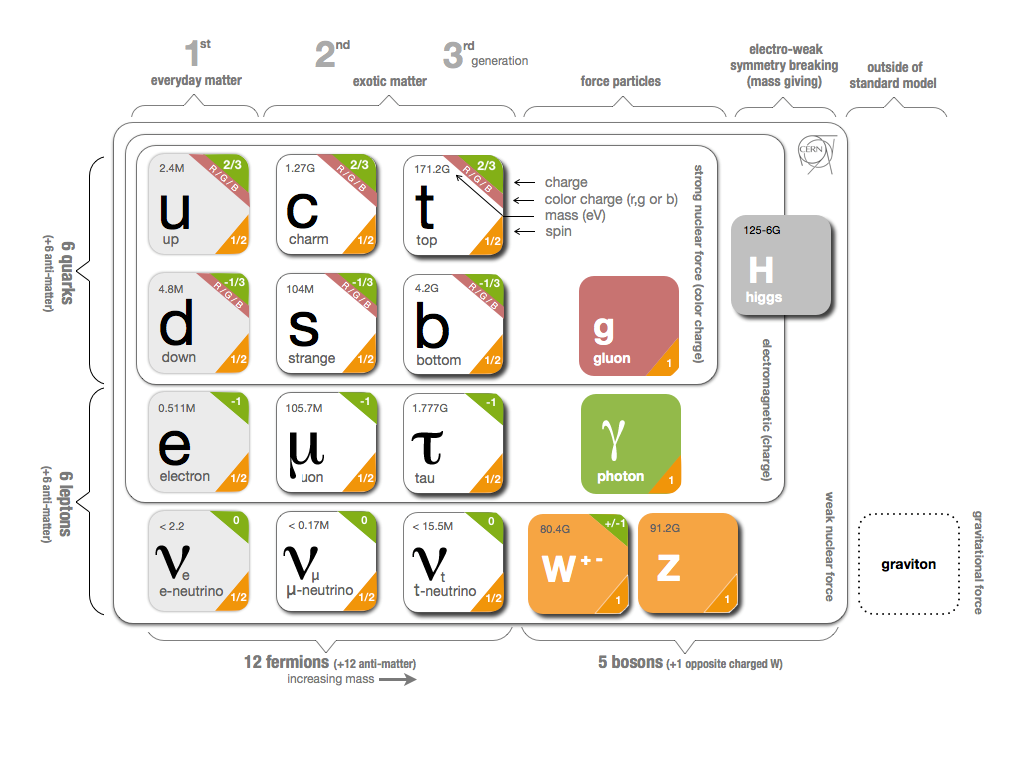
\includegraphics[width=\textwidth]{Figures/FromOnline/SM.png}
    \caption{An overview of the particles in the Standard Model \cite{SMpicture}.}
    \label{fig:SM}
\end{figure}

\subsection{Fermions}
If we look at figure \ref{fig:SM}, we can see that there are 12 different fermions split up in two groups called quarks and leptons, which again are split up into three generations. The lightest quarks and leptons are in the first generation, and the most massive quarks are in the third generation. All of the fermions are $\frac{1}{2}$-spin particles and differ by mass and electric charge. They also obey the Pauli exclusion principle, which means that only one fermion can occupy a given quantum state for any given set of quantum numbers.

\subsubsection{Quarks}
We have six different quarks \cite{thomson} in the SM, and they differ by mainly mass, but also charge (color charge, in addition to electrical charge). All the up-type quarks, which are the three quarks in the first row in figure \ref{fig:SM}, have charge +2/3 and all the down-type quarks, which is in the second row in figure \ref{fig:SM}, have charge -1/3. Since they carry a non-zero electric charge, they interact via the quantum electrodynamics (QED). They can also interact with the weak force which allows all possible combinations in doublets, where they differ by one unit of charge. 

\begin{align}
    \binom{u}{d} \text{,  } \binom{u}{s} \text{,  } \binom{u}{b} \text{,  } \binom{c}{d} \text{,  } \binom{c}{s} \text{,  } \binom{c}{b} \text{,  } \binom{t}{d} \text{,  } \binom{t}{s} \text{,  } \binom{t}{b}
\end{align}

The two quarks in the first generation, namely up (u) and down (d), are the constituents of the protons (uud) and neutrons (ddu) - which then combine in various ways to form atomic nuclei. The second and third generation of quarks (charm, strange, top and bottom) are more massive than the quarks in the first generation (up and down). Since the quarks in the second and third generations are more massive, they need more energy to exist and will therefore decay to lighter particles very fast. Quarks are the only known particles that interact with all the fundamental forces. They also carry color charge in addition to electrical and weak charge, which allows them to couple to different gluons through the strong interaction in quantum chromodynamics (QCD).  

Note that the quarks can be described by either mass eigenstates corresponding to the free-propagating Hamiltonian, or weak eigenstates corresponding to the way they interact under the weak interaction. Those sets of eigenstates do not coincide but are instead related to each other by the CKM matrix \cite{thomson}. 




\subsubsection{Leptons}
Leptons are the other six fermions in the SM. Like quarks, they come in three generations and are arranged in doublets, as shown below.

\begin{align}
    \binom{\nu_e}{e^-} \text{,  } \binom{\nu_\mu}{\mu} \text{,  } \binom{\nu_\tau}{\tau}
\end{align}

They also differ by mass and electric charge where the lower component has charge -1, and the upper has no charge. Because of that, neutrinos only interact with weak bosons, while for the electron, muon and, tau, electromagnetic interactions are also possible. In the SM the neutrinos are assumed to be massless, but we know from neutrino oscillation experiments that this is not true. However, exactly how the neutrinos acquire mass and why they are so much lighter than all of the other particles in the SM is not yet understood. 

Analogously to quarks, fermion mass and weak eigenstates do not coincide and they are related by the PMNS matrix \cite{thomson}. This phenomenon provides an explanation of neutrino oscillations, where after some distance from the interaction point we measure a different neutrino flavor. 


\subsection{Bosons}
On the right-hand side of figure \ref{fig:SM}, the integer spin particles (spin-1, spin-0) known as bosons \cite{thomson} are shown. Bosons follow Bose-Einstein statistics and contain the force carriers for the electromagnetic force, the weak force, and the strong force. If gravity was included in the Standard Model, it would have been through an extra boson, the graviton ($G$).

\subsubsection{The strong nuclear force}
The strong nuclear force is mediated by the gluon (g) \cite{thomson} and couples to the three color charges r, g, b. Moreover, as suggested by the name, it has a very strong coupling to quarks, and it is responsible for the fact that quarks do not appear as free, unbounded particles. The gluon is massless, and unlike the other forces, it can couple with itself, as you can see in the Feynman diagrams\footnote{Feynman diagrams are a way to graphically represent interactions between particles.} in figure\ref{fig:gluon_self_int}.

\begin{figure}[H]
    \centering
    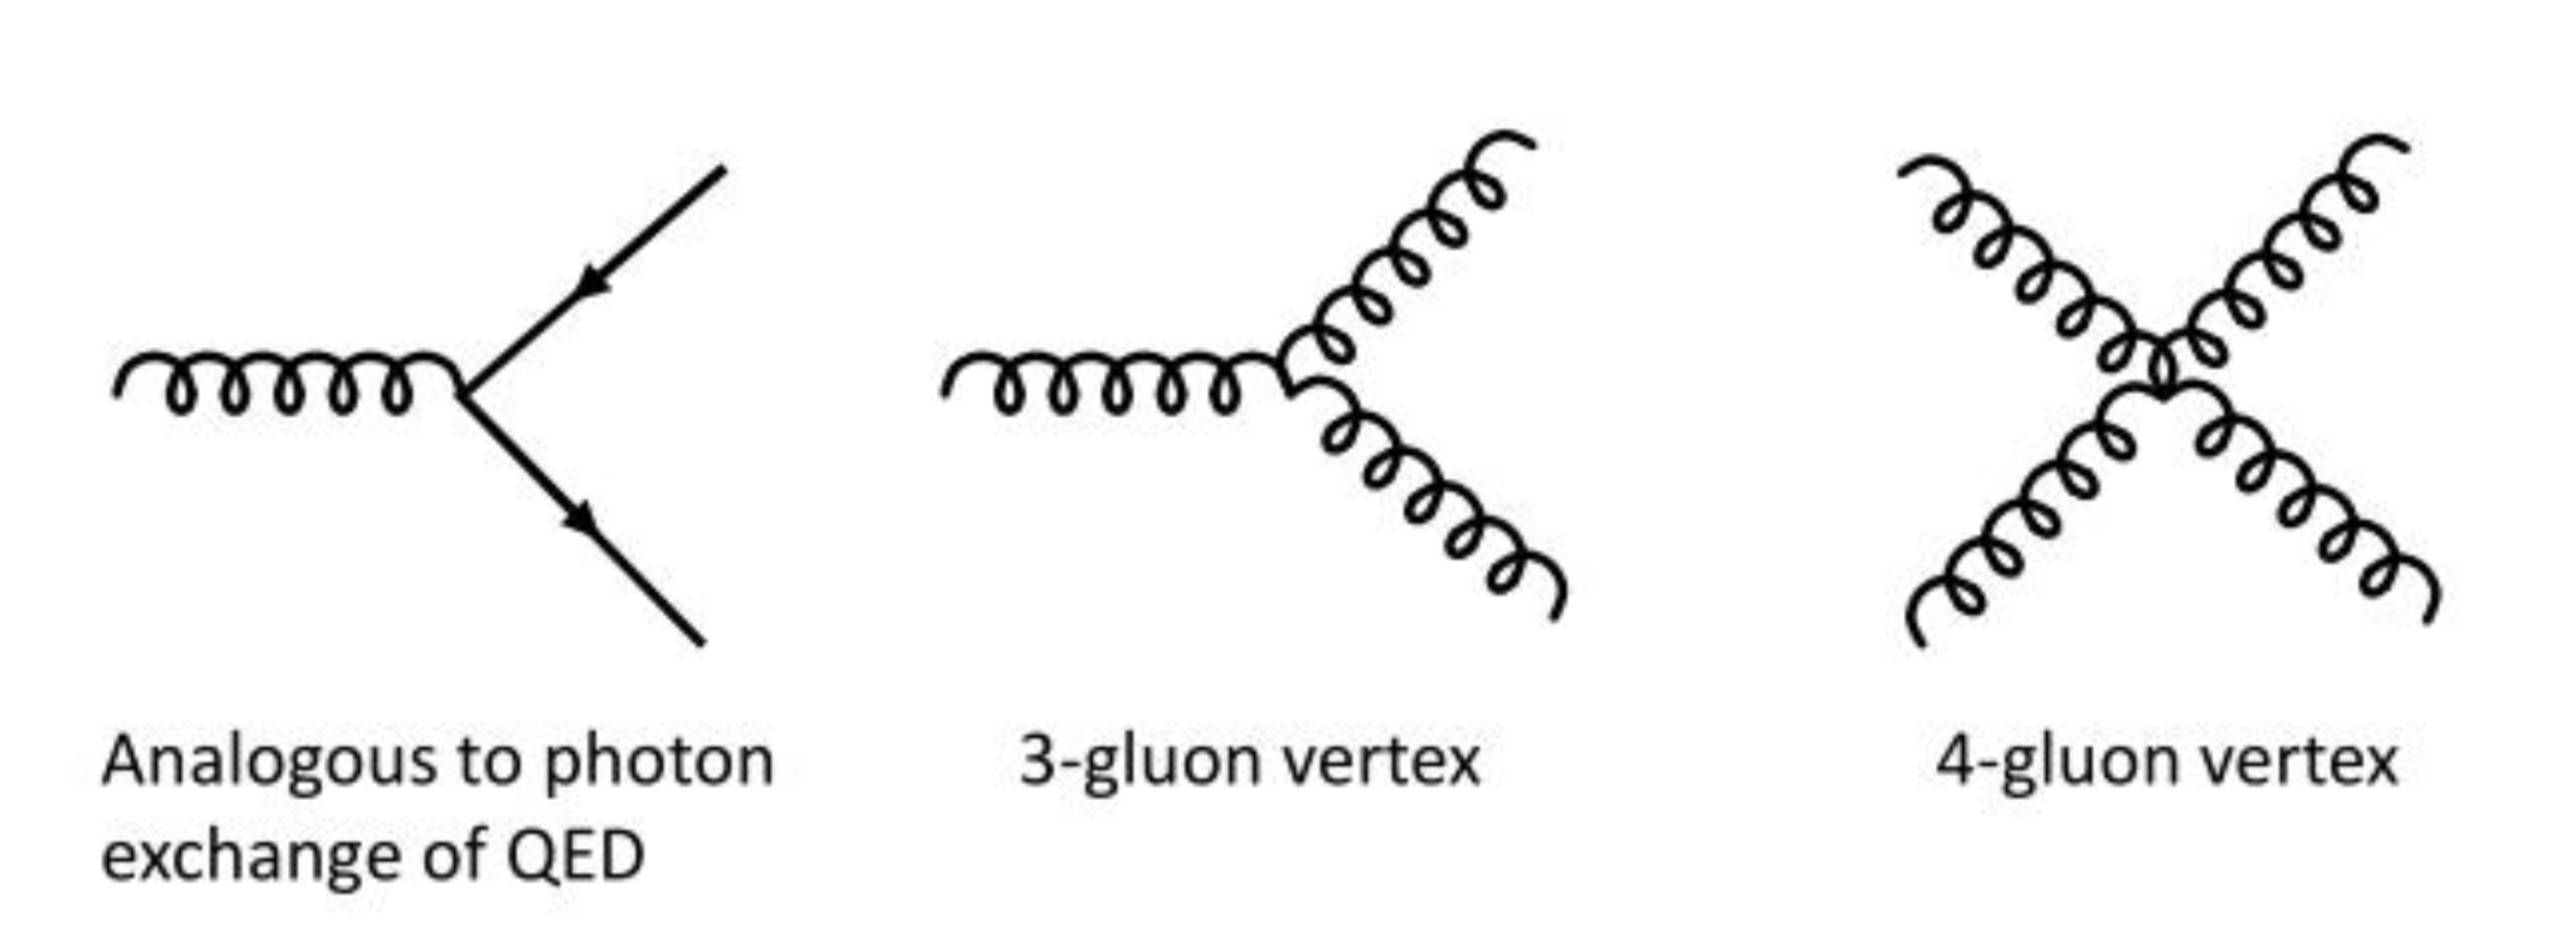
\includegraphics[width = \textwidth]{Figures/FeynmanDiagrams/gluon.pdf}
    \caption{Feynman diagrams for the strong force vertices, where the curly lines represent the gluons \cite{STRONGforce}.}
    \label{fig:gluon_self_int}
\end{figure}

\subsubsection{The electromagnetic force}
The electromagnetic force is mediated by the photon ($\gamma$) \cite{thomson} and couples to all fermions with electric charge, namely all the quarks and leptons except for the neutrinos. As for the gluon, it has no mass, but since it is electrical neutral it cannot couple to itself. 

\begin{figure}[H]
    \centering
    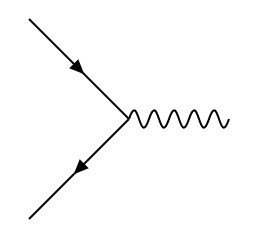
\includegraphics[width = 0.4\textwidth]{Figures/FeynmanDiagrams/photon.png}
    \caption{A Feynman diagram of the electromagnetic vertex, where the wiggly line represent the photon \cite{EMforce}.}
    \label{fig:my_label}
\end{figure}

\subsubsection{The weak nuclear forces}
The weak nuclear forces are mediated by the $W^\pm$-bosons and the $Z^0$-boson \cite{thomson}. They couple to all particles in the SM, and unlike the other force particles, they have mass. This feature is explained in the GWS model \cite{Xin2007GlashowWeinbergSalamMA} through a spontaneous symmetry breaking due to a non-zero vacuum expectation value that adds an extra degree of freedom to otherwise massless force carriers. It is also the only interaction known to allow flavor change, which means that e.g., an up quark can become a down quark or a muon become an electron as shown in figure\ref{fig:weak_force_FD}. 

\begin{figure}[H]
    \centering
    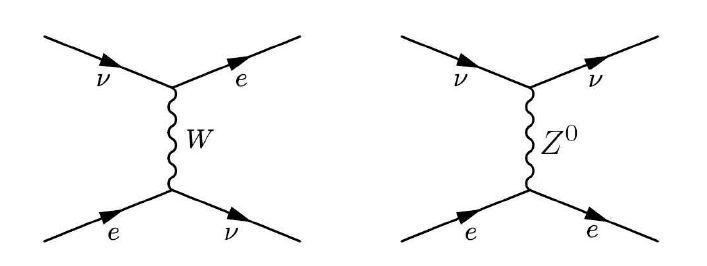
\includegraphics[width = 0.8\textwidth]{Figures/FeynmanDiagrams/weak.png}
    \caption{Feynman diagrams of the weak force vertices \cite{WEAKforce}.}
    \label{fig:weak_force_FD}
\end{figure}


\subsubsection{SM symmetries and the Higgs boson}
Formally, the three interactions in the nature are related by to three different symmetry groups. The SM is represented by

\begin{equation}
    U(1)_Y \otimes SU(2)_L \otimes SU(3)_C,
\end{equation}

where $U(1)_Y$ is the symmetry associated to the hyper charge $Y$, $SU(2)_L$ the transformations acting on the left-handed isospin doublets and $SU(3)_C$ are the ones acting on color triplets. The physical bosons $\gamma, Z^0, W^\pm$ are not the mediator associated to the single symmetry groups, but are instead a linear combination of those states explained by the spontaneous symmetry breaking leading to the electroweak theory. 

The final piece, the Higgs boson (H) \cite{thomson}, that was missing in the SM was discovered in 2012 at CERN \cite{Higgs_ATLAS, Higgs_CMS}. The discovery gives increased credence to the SM and explains why the weak force carriers, $Z^0$ and $ W^\pm $, have mass. The fermion masses, except for neutrinos, can also be explained by couplings to the Higgs boson. 




\section{Beyond the Standard Model}
As mentioned earlier, the SM is not enough to explain every phenomenon in physics and the universe. There are several challenging sides of the SM; for instance, the parameters used in the model are made to fit experimental data and do not come from theoretical principles. 
The SM does not offer a solution to unifying the framework with gravity, the hierarchy problem (a large discrepancy between aspects of the weak force and gravity), or the fact that neutrinos oscillate. The SM does not explain what dark energy and dark matter are either.  

Given these shortcomings, various other theories have been proposed to try and solve some of the open questions. Several expansions of the Standard Model exist, and there are pros and cons to every one of them. Furthermore, even though the search has been going on for years, no concluding scientific evidence has been found to favor one particular SM extension over another. Below we detail an outline of one possibility, SUSY.

\subsection{Supersymmetry}
\label{sec:SUSY}
One of the theories we are looking at is Supersymmetry (SUSY) \cite{sleptonexclusion}. SUSY relates the integer spin particles (bosons) and the half-integer spin particles (fermions) in the SM to half-integer spin particles and integer spin particles in SUSY. These new particles are named "super particles", or \textit{sparticles}, because SUSY predicts a supersymmetric partner for all of the SM particles. An illustration of the particles in SM and their superpartner in SUSY can be found in figure \ref{fig:smandsusy}.

\begin{figure}[H]
    \centering
    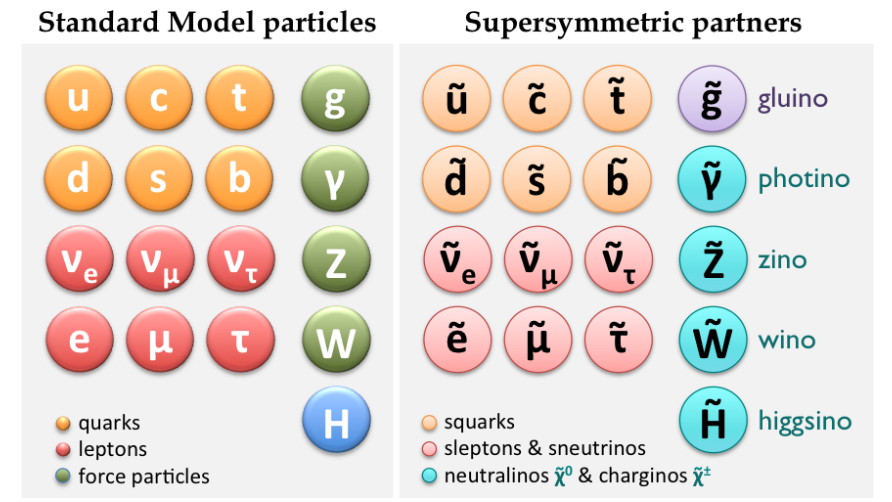
\includegraphics[width = 0.75\textwidth]{Figures/FromOnline/susy_particles.png}
    \caption{An illustration of the content of particles in the SM and sparticles in SUSY \cite{SUSYpic}.}
    \label{fig:smandsusy}
\end{figure}

In SUSY, we do not have to introduce any new gauge groups, which means we do not have to handle any new fundamental forces. Because of this we can, in a way, say that we can describe supersymmetry with the help of a supersymmetry operator $Q$ (shown in equation \ref{eq:SUSY}) that alters the spin of the SM particles by $1/2$ and commutes with the gauge transformations of the SM. 

\begin{equation}
    \label{eq:SUSY}
    Q\ket{fermions} = \ket{bosons} \text{,   }  Q\ket{bosons} =\ket{fermions}
\end{equation}

SUSY possibly provides a solution to the SM's hierarchy problem, which involves the need to reconcile the very different scales of electroweak symmetry breaking and the gravitational Planck scale ($M_{Pl}$). SUSY allows the unification of the electroweak and strong interactions, proposes dark matter particle candidates, and requires five Higgs bosons (three neutral and two charged ones). 




\begin{comment}

We know that the sparticles differ from the particles by $1/2$ spin, but that is almost the only difference when 

Supersymmetry allows for a connection between fermions and bosons by introducing a new set of particles. Each SM-particle has a sparticle, equal in all quantum numbers except a half unit difference in spin, i.e. the SM-fermions get a bosonic superpartner (denoted by an "s" in front of the name, e.g. electron $\rightarrow $ selectron) while the SM-bosons get a fermionic superpartner (denoted by "-ino" added to the end of the name, e.g. $W \rightarrow$ wino). All sparticles are denoted by a tilde above their symbol, e.g. selctron ($\tilde{e}$). If SUSY is a valid extension of the Standard Model, we know that it must be a broken symmetry where the particles and sparticles must have different masses although all the quantum numbers are equal. The sparticles must be heavier than their partner, or else we would already have been able to detect them in particle detectors, such as the ATLAS experiment. 

Supersymmetry offers a solution to the hierarchy problem, and when imposed as a local symmetry, gravity. According to Einsteins mass-energy equivalence equation ($E = mc^2$), we should be able to produce any particle in the universe as long as we collide them with a high enough amount of energy.





:
Production of pairs of sleptons, hypothetical supersymmetric partners of leptons, in the process pp→~l+~l-→ l+l-+χχ, where the DM candidate χ is the lightest neutralino (a mixture of photino, zino and higgsino), leading to a pair of leptons (e⁺e⁻ or µ⁺µ⁻) and missing transverse energy (MET).







The process I am looking at in this project is direct slepton production as shown in the Feynman diagram in figure \ref{fig:slepslep}. Production of pairs of sleptons, hypothetical supersymmetric partners of leptons, in the process $pp\rightarrow \tilde{l}^+\tilde{l}^- \rightarrow l^+l^-+ \chi \chi$, where the DM candidate $\chi$ is the lightest neutralino (a mixture of photino, zino and higgsino), leading to a pair of leptons ($e^+ e^-$ or $\mu^+ \mu^-$) and missing transverse energy (MET).



The same final state (l+l-+MET) above may be due to the production of a pair of lightest charginos χ±1 , a mixture of the wino (W-superpartner) and the charged higgsino (charged Higgs superpartner), through the process pp→ χ+1χ-1, followed by (i) slepton-mediated ( ~l+~l-/~ν~ν → l+l-  + ννbar + χχ) or (ii) W-mediated (W+W-→l+l-  + ννbar +χχ) decays into leptons and MET.



\textbf{To do:}
\begin{itemize}
    \item Fixing the hierarchy problem
    \item Superpartners
    \item Legg
\end{itemize}
\end{comment}





\subsection{Dark matter}
\label{sec:DM}
We have many unanswered mysteries in physics today, but probably the greatest one is the nature of dark matter (DM) \cite{monoZexclusion}. In the previous section's SUSY processes, we have seen that a "consequence" of SUSY may give us some viable DM candidates, namely the LSP neutralino. In this section, we will look at DM particles produced in a more simplified model; that is, a non-supersymmetry model. In this model, we assume that we have a DM mediator in addition to the DM particles in the final state. This mediator can be, among others, a scalar or a vector. This process's signature consists of detecting a well known SM particle recoiling against missing energy-momentum carried away by DM particles. 





\begin{comment}
\textbf{To do:}
\begin{itemize}
    \item Les om mørk materie. Du har jo strengt tatt ikke litt peiling engang..
    \item 
\end{itemize}


\begin{figure}[H]
    \centering
    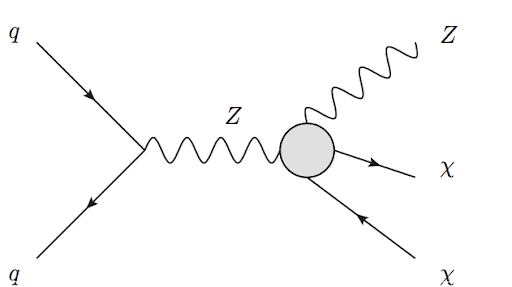
\includegraphics[width = 0.5\textwidth]{Figures/FeynmanDiagrams/monoZFeynman1.png}
    \caption{Caption}
    \label{fig:monoZFeynman1}
\end{figure}
\end{comment}







%\chapter{LHC and ATLAS}
\label{sec:LHCandATLAS}
The data used in this thesis comes from the Atlas experiment at LHC. In this chapter,  a brief introduction to both the experiment and the accelerator will be presented. We will also get a small incite to the organization behind the experiment and the accelerator, namely CERN. 

\section{CERN}
\label{sec:cern}

The European organisation for nuclear research, CERN, started as a research facility on mainly nuclear physics. It was built on the border between France and Switzerland near Geneva in 1954. CERN have 22 member states, where Norway is one of the founding members, but it welcomes people from all over the world to take part in the different experiments and accelerator development. 

CERN quickly became the biggest and leading research centre in particle physics as well, and the most famous discoveries done at CERN are the discoveries done with high energy particle collisions. To mention some of the discoveries done at CERN we have weak neutral currents that are mediated by the hypothetical Z-boson in 1973 \cite{Zmed} and of course the discovery of the actual Z-boson and the W-boson mediators of the weak force in 1983/84 \cite{WZ1, WZ2, WZ3}. The most recent discovery is certainly that of the Higgs boson \cite{Higgs_ATLAS, Higgs_CMS} in 2012 by the ATLAS and CMS experiments, which also was the last piece to confirm the SM.

Through out the years there have been built many different accelerators at CERN. Among others the Super Proton Synchrotron (SPS) accelerated protons and antiprotons and allowed the UA1 and UA2 experiments to discover the Z- and W-bosons. The Large electron positron collider (LEP) was built in a 27 km long tunnel 100 m below ground and was definitively the biggest accelerator at the time. LEP allowed important SM precision measurements. The last run at LEP was done in 2000 paving the road for the start of building the Large Hadron Collider (LHC) which is the accelerator that produced proton-proton collisions data recorded by the ATLAS detector and which have been used to obtain the data for this thesis. 

\section{LHC - Large Hadron Collider}
\label{sec:LHC}

The Large Hadron Collider (LHC) \cite{LHCcern} is a 27km long particle accelerator 100 meters below ground and it is the most powerful of its kind in the world. Since LHC replaced LEP, the tunnel already existed which made the building a bit less comprehensive. The collider consists of superconducting magnets with accelerating structures to boost the proton velocity close to the speed of light, in an environment cooled down to 1.85K (-271.3$^o$C) to insure superconductivity. The LHC collider is shown in figure \ref{fig:LHC} as part of a complex of CERN accelerators. 

\begin{figure}[H]
    \centering
    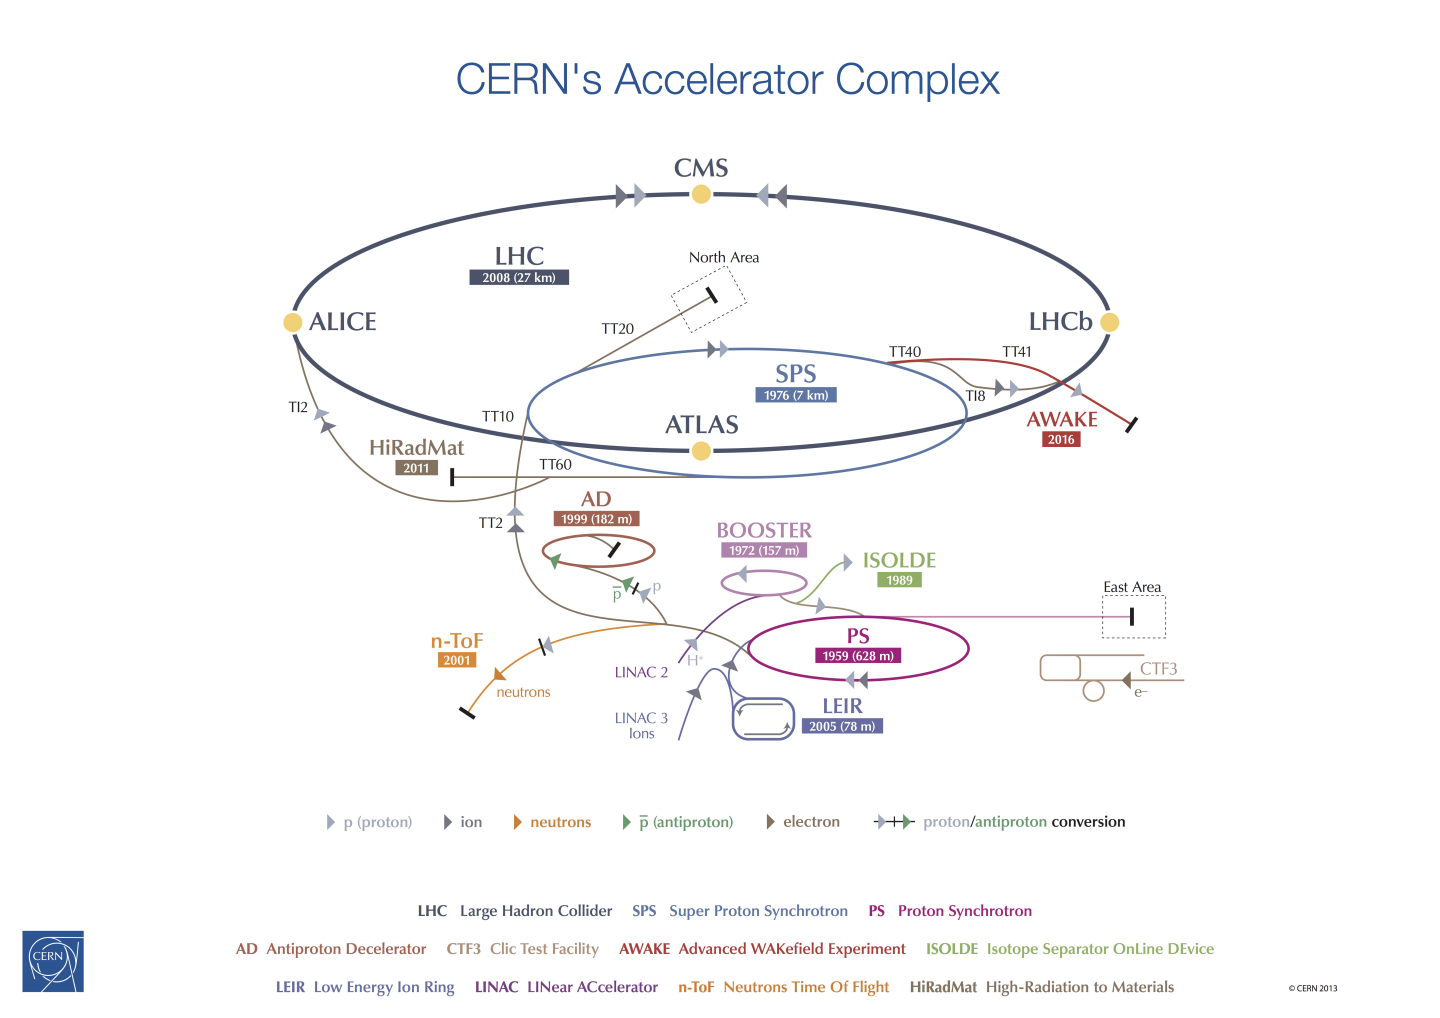
\includegraphics[width=\textwidth]{Figures/FromOnline/Poster-2013-377.jpg}
    \caption{An illustration of the accelerator complex at CERN \cite{LHCpic}}
    \label{fig:LHC}
\end{figure}

The protons extracted from a hydrogen bottle go through smaller accelerators to gain more energy before they in the end are sent in opposite directions into the LHC which is the big circle we can see in figure \ref{fig:LHC}. The particles get accelerated to about 99.99\% of the speed of light and a maximum energy of 6.5 TeV. In the end the two beams of protons will collide in the centre of four experiments around LHC, which are marked with yellow dots in figure \ref{fig:LHC}, namely ATLAS, ALICE, CMS and LHCb. 

The different experiments focus on different research goals. ATLAS (A Toridal LHC ApparatuS) and CMS (Compact
Muon Solenoid) are multipurpose detectors mainly focusing on SM measurements and searches for new physics, i.e. discovery of new particles and phenomena, e.g. SUSY. The last big achievement of ATLAS and CMS is the discovery of the Higgs boson. While ALICE (A Large Ion Collider Experiment) focuses on heavy ion collisions with lead-lead and lead-proton to study the quark-gluon plasma, LHCb (Large Hadron Collider beaty) focuses on processes related to b-quarks to precisely measure CP violation and oscillation phenomena. 

At the LHC we focus on proton-proton collisions (and heavy ion collisions) to study various high energy final states via electroweak and strong interactions with the hope to discover new phenomena. The internal structure of the proton allows to register a large amount of events in a single collision and thus collect a wider statistics for our experiments. The number of collisons per area per second is defined thorugh the luminosity $\mathscr{L}$, given by

\begin{equation}
    \label{eq:lumi}
    \mathscr{L} = f \frac{n_1 n_2}{4 \pi \sigma_x \sigma_y},
\end{equation}

where f is the crossing rate of the proton bunches, $n_i$ is the number of colliding particles in each bunch and $\sigma_{x,y}$ is the spread of the bunch along the x- and y-direction.  

Using the integrated luminsoty over time we can find the number of interactions $N$ in our dataset. This is given by  
\begin{equation}
    \label{eq:intLumi}
    N = \sigma \int \mathscr{L}(t) dt, 
\end{equation}

where $\sigma$ is the cross section for a certain process. 

As the luminosity gets higher, we have more collisions happening in the detector. This gives us a lot of interactions at the same time, which can introduce further systematic uncertainty. This phenomenon is called \textit{pile-up}. We need to consider this to know which particles in the final state comes from which interaction. This is a constantly evolving problem since we are further developing the LHC infrastructures and apparatus towards higher and higher luminosity, e.g. HL-LHC (High Luminosity LHC).








\section{The ATLAS detector}
\label{sec:ATLAS}
\begin{comment}


\begin{itemize}
    \item Skriv kort om ATLAS
    \item Tracking
    \item luminositet osv
    \item luminosity $10^{34} cm^{-2}s^{-1}$ for proton-proton
    \item upgrade to HL-LHC
    \item size
    \item figure of tracks
    \item coordinate system and navngiving og nyttige variabler: lumi og pileup og number of interations and rate.
    \item origin of the coordinate system: nominal interaction point
    \item $\phi$ og $\Theta$
    \item transverse og alle er definert i x-y-planet
    \item pseudo rapidity
    \item $\Delta R_{ll}$
    \item INNER DETECTOR:
    \item Hvor den er
    \item Exposed for mye radiation og derfor må vi oppgradere nå
    \item scheduled at 2024, men vil bli utsatt (som er neste oppgradering igjen)
    \item Tracker de første bevegelsene av partiklene som er skapt i kollisjonen og må være veldig presis. 
    \item inner detector er inni et 2T magnetfelt som kommer fra the central solenoid. Som er med på å hjelpe oss å tracke partikler fordi ladde partikler vil bendes av mahnetfeltet.
    \item bilde av inner detector
    \item CALORIMETERS:
    \item Du må vite energien for å rekonsturere partikler fra kollisjonen. Calorimeteret måler hvor mye energi partikkelen legger igjen når den møter detektormaterialet.
    \item To er brukt: one EM calorimeter og hadronic calorimeter
    \item Bilde av begge calorimeters (en figur)
    \item Vi trenger calorimeters for å tracke ET og det er viktig for BSM.
    \item EM cal:
    \item for å tracke electrons og photons 
    \item HAD cal:
    \item Outside of EM og den er bygd for å tracke hadrons og hadronic showers. Legg in hva en shower er. cascade decay.
    \item jet reconstruction og met
    \item MAGNETS:
    \item ATLAS består av to magnetsystemer: a central solenoid og a barrel (symmetrisk rundt beam axis) toreoid og two end-cap toreoids. 
    \item MUON system:
    \item basert på magnet deflection of muon tracks. Muon kammerne eksisterer rundt hele detektoren hvor den går rundt beam aksen og de ytterste ligger i x-y-planet. Ligger som en tønne rundt beam aksen og med lokk på endene. barrel region og end-cap regions.
    \item Triggers and data acquesition? 
    
\end{itemize}
\end{comment}
The ATLAS \cite{ATLAS} detector is a massive 44 m long detector, 25 m in diameter and weighing about the same as the Eiffel tower ($\sim 7000$ tons). It is designed to handle proton-proton collisions up to 14 TeV with a luminosity of a few times $10^{34}$cm$^{-2}$s$^{-1}$. We can see an illustration of the whole detector in figure \ref{fig:atlas}, where the most important components are marked. 


\begin{figure}[H]
    \centering
    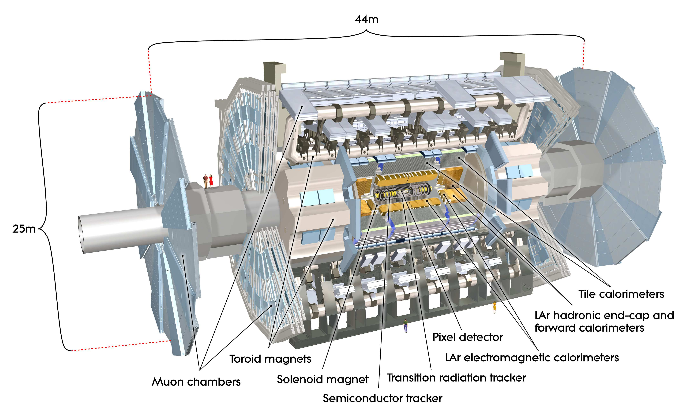
\includegraphics[width = \textwidth]{Figures/FromOnline/ATLAS.png}
    \caption{An illustration of the ATLAS detector \cite{ATLAS}.}
    \label{fig:atlas}
\end{figure}

The detector is built up in three main layers. Two inner tracking layers, that provide the information about particle trajectories and allow to determine, with good resolution, the interaction point and secondary vertices. The inner detector is composed of a pixel and strip silicon tracker and a transition radiation tracker. A good tracking resolution is in fact needed for particle identification purposes: the whole inner detector is inserted in a solenoid magnet that generates a magnetic field along the beam direction. The bending trajectory of charged particles in magnetic field leads to a determination of momentum and electric charge of the particles.

The tracker is followed by two layers of calorimeters. The innermost is the electromagnetic calorimeter and consists of alternating layers of lead and liquid argon. The purpose of the layer is to stop photons, positrons and electrons by inducing electromagnetic showers that allow to measure the energy of the particles. The outer calorimeter is the hadronic calorimeter, composed of three different detectors. The hadrons produced in the event interact with the calorimeter material and produce hadronic showers, also called \textit{jets}, that lose their whole energy in this layer. 

The outer layer consists of the muon chambers, which surround the whole detector as a barrel with two end-caps at the edges. Muons are the only detectable particles that are able to travel through all the other layers, only depositing a minimum ionisation energy. 

All the particles we cannot track in the detector layers are referred to as missing energy/momentum, essentially inferred from energy-momentum conservation and the measurement of all visible particles the energy difference $E_{miss} = -\sum_i E_i$ and $\Vec{p}_{miss} = -\sum_i \Vec{p}_i$. 

A sketch of the layers presented above is shown in figure \ref{fig:tracks}.

\begin{figure}[H]
    \centering
    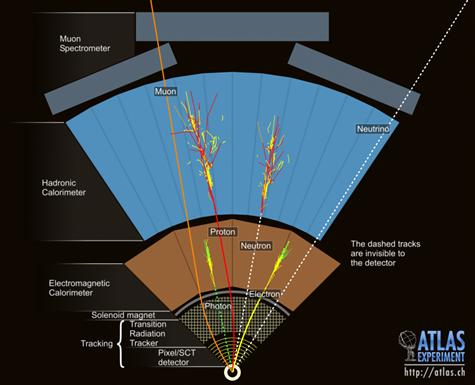
\includegraphics[width = 0.8\textwidth]{Figures/FromOnline/tracks.jpg}
    \caption{An illustration on how we see the tracks of the different particles in the detector \cite{tracks}.}
    \label{fig:tracks}
\end{figure}


\subsection{Variables and coordinates}
Combining information from the different layers it is possible to calculate different variables and identify the different particle species. We have two particles with opposite momentum $p$ in each collision and therefore we are interested only in the transverse direction, since the longitudinal momentum of the final states is negligible at such high energies. The energy deposited by the particle is measured by the detector and combined with the tracking information to have the vector quantities of $p_T$ and $E_T$ connected by the invariant mass m of the particle by the relation $p_T^2 = E_T^2 - m^2$. As mentioned before we can measure the energy difference between before and after the collision that gives us the \textit{missing transverse energy} (MET/$E_T^{miss}$). 

It is also useful to introduce the coordinates used within the detector to describe an event. A sketch is shown in figure \ref{fig:coordsys}. The $z$-coordinate is defined by the beam direction and the $x,y$-coordinates define the transverse plane. In addition we have the two angles $\theta$ and $\phi$, respectively the angle between the particle and the $z$-axis and the one with respect to the $x$-axis. Note that instead of referring to the coordinate $\theta$ it is common to introduce the pseudorapidity $\eta$ defined as 

\begin{equation}
    \eta = -\ln \tan \bigg(\frac{\theta}{2}\bigg).
\end{equation}

\begin{figure}[H]
    \centering
    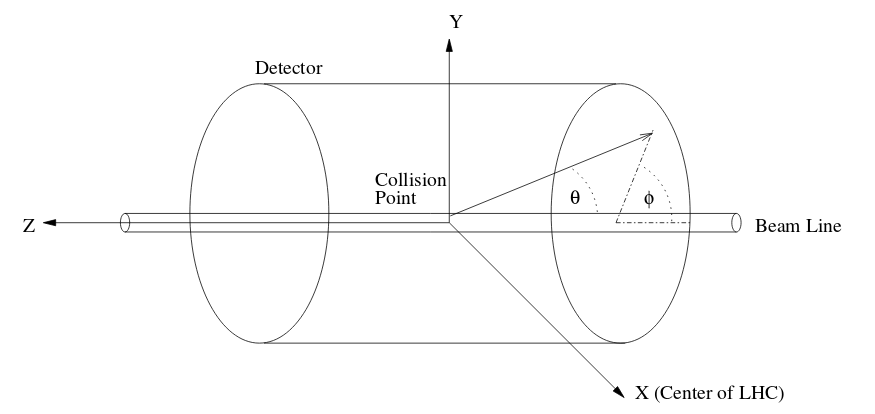
\includegraphics[width = \textwidth]{Figures/FromOnline/coordinatesystem.png}
    \caption{An illustration of the coordinate system inside the detector\cite{coordinatesystem}.}
    \label{fig:coordsys}
\end{figure}

The other variables we are considering in this thesis are listed below

\begin{itemize}
    \item $m_{l^+l^-}$ is the invariant mass of the lepton pair in the final state, defined as 
            \begin{equation}
                m_{l^+l^-} = \sqrt{(E_{l^+} + E_{l^-})^2 - (\mathbf{p}_{l^+} + \mathbf{p}_{l^-})^2}.
            \end{equation}
    \item $m_{T2}$ is the stransverse mass \cite{sleptonexclusion} and is used to describe the masses of a particle pair that is assumed to have decayed to one visible and one invisible particle. It is defined as 
    \begin{equation*}
        m_{T2}(\mathbf{p}_{T,1}, \mathbf{p}_{T,2}, \mathbf{p}_{T}^{miss}) = \min_{q_{T,1} + q_{T,2} = p_T^{miss}} \bigg\{\max\big[m_T(\mathbf{p}_{T,1}, \mathbf{q}_{T,1}), m_T(\mathbf{p}_{T,2}, \mathbf{q}_{T,2})\big]\bigg\},
    \end{equation*}
    where $m_T$ is the transverse mass (defined as $m_T = \sqrt{2 |\mathbf{p}_{T,1}| \cdot |\mathbf{p}_{T,2}| \cdot \big(1-\cos(\Delta\phi)\big)}$), $\mathbf{p}_{T,1}$ and $\mathbf{p}_{T,2}$ are the transverse momentum vectors of the two leptons in the final state, and $\mathbf{q}_{T,1}$ and $\mathbf{q}_{T,2}$ are vectors with $\mathbf{p}_{T}^{miss} = \mathbf{q}_{T,1} + \mathbf{q}_{T,2}$. 
    \item  $H_T$ is the scalar sum of the $p_T$ of the jets and leptons we have selected.
    \item  $\Delta \phi (\Vec{p}_T^{ll}, E_T^{miss})$ is the azimuthal angle difference between the two lepton system and the missing transverse energy.
    \item $\Delta R_{ll} = \sqrt{(\Delta\phi_{ll})^2 + (\Delta \eta_{ll})^2}$ is the distance between the two leptons in the final state.
\end{itemize}


   
  
    







\begin{comment}


\begin{figure}[H]
    \centering
    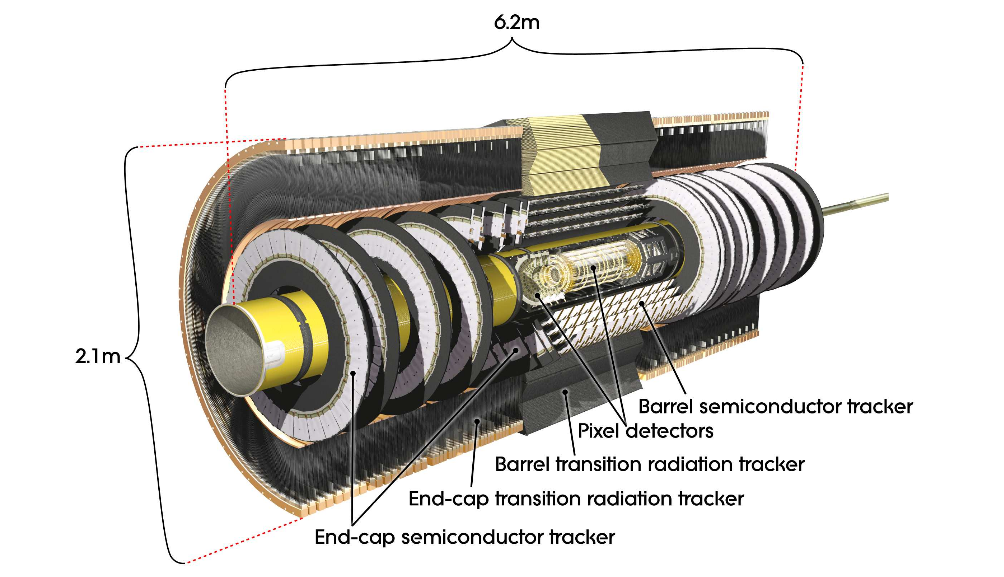
\includegraphics[width = \textwidth]{Figures/FromOnline/innerdetector.png}
    \caption{An illustration of the inner detector \cite{innerdetector}.}
    \label{fig:innerdet}
\end{figure}


\begin{figure}[H]
    \centering
    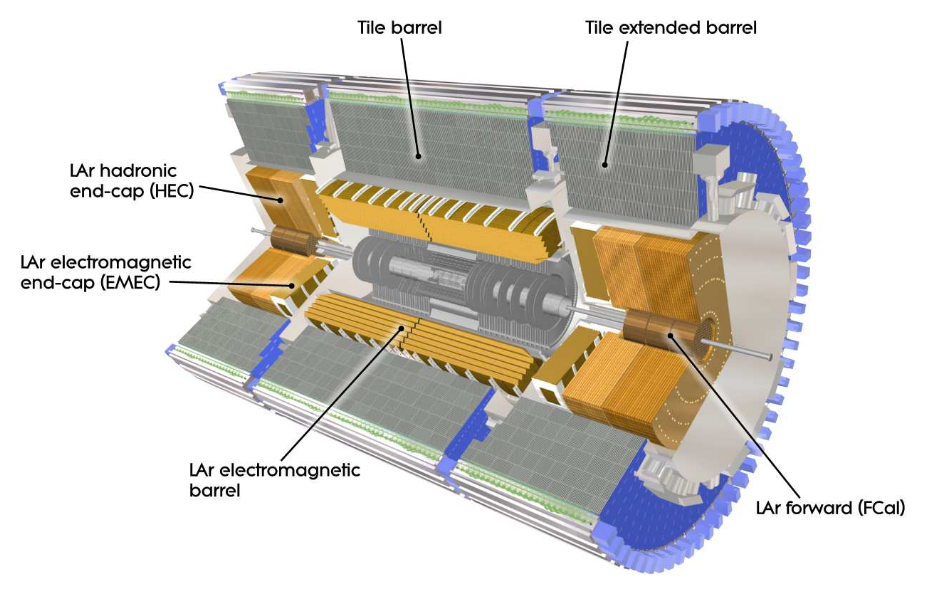
\includegraphics[width = \textwidth]{Figures/FromOnline/calorimeters.png}
    \caption{An illustration of the calorimeters \cite{innerdetector}.}
    \label{fig:calori}
\end{figure}


\begin{figure}[H]
    \centering
    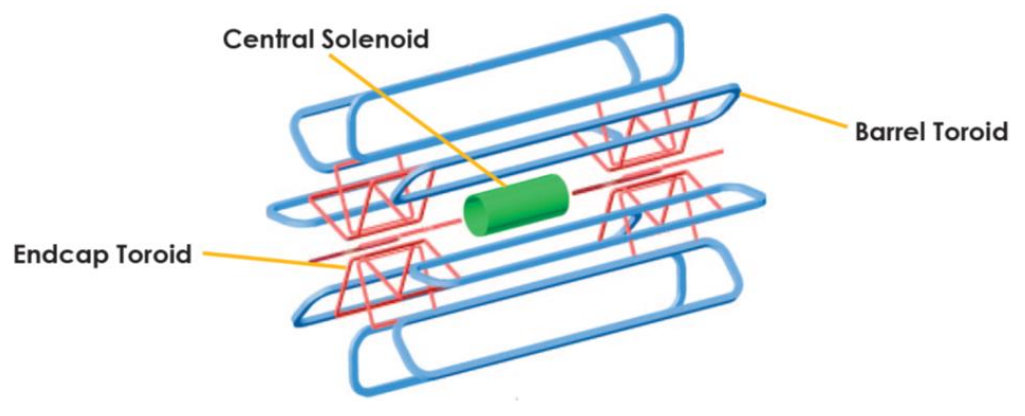
\includegraphics[width = \textwidth]{Figures/FromOnline/magnetsystem.png}
    \caption{An illustration of the magnet systems \cite{magnetsystem}.}
    \label{fig:magnetsys}
\end{figure}
\end{comment}



















\section{Computing infrastructure}
The results obtained in this thesis have been very comprehensive when it comes to computing power. It has not been possible to run the code on a regular computer because of not enough CPU's and memory. Because of these problems we have borrowed a server at Simula Research Laboratory, where we got to use the Experimental Infrastructure for Exploration of Exascale Computing. This is a computer with two sockets with 8 cores/CPU's, which again have two threads. This gives us in all 32 virtual CPU's (16 physical) because of hyper-threading in each CPU. It also have 60 GiB\footnote{GiB is Gibibyte instead of regular gigabyte and is simply a unit byte for digital information and means 2 to the power of 10 (kiB), 20 (MiB), 30 (GiB), 40 (TiB) and 50 (PiB).} memory, which have been crucial to handle the data used in ML. With this setup, the import of the data, training and testing have taken approximately 12-13 days, where 7 of these are just for importing the data. All together we have trained and tested 72 ML models (36 BDTs and 36 NNs) and the data sets we have been working on have been massive, where the memory have come in handy. 

In the final run-up of this thesis we have used a server that is in possession of the HEPP-group at UiO. It is a Supermicro Ultra Server with both GPU's and CPU's, but we have only taken advantage of the CPU's in this thesis. This server is a much more powerful computer than the one borrowed at Simula. It has two sockets with 128 cores/CPU's, which also have two threads in each CPU. This gives us a total of 256 virtual CPU's. It also has 2 TiB memory, which has resulted in that we could import the data in several parts and be done in around 3 days instead of a week. And we have been able to train around 18-20 ML models at the same time instead of 1-2 which was the maximum for the Simula server. 
\chapter{Search for Supersymmetry and Dark Matter in Events with Dileptons and Missing Energy}
\label{sec:CandCanalysis}

%Beskriv prosessene her istedet for i teori og motiver hvordan partiklene er produsert. 

This chapter will introduce the processes we are searching for in the analysis, how the signal and background samples are produced, and how we do a traditional analysis when searching for new particles or phenomena in LHC data. We will show the results obtained by the ATLAS collaboration and compare the results with ours. 



The processes we are interested in looking at in this thesis involve superpartners of leptons, gauge bosons, and the Higgs boson. Besides this, we will look at a dark matter particle candidate, which is predicted to be the lightest supersymmetric particle (LSP).  This thesis looks at proton-proton collisions with final state two leptons and missing transverse energy (MET/$E_T^{miss}$). The SUSY processes we are looking at are direct slepton production, chargino production with slepton/sneutrino-mediated-decays and with W-boson-mediated-decays. 


In figure \ref{fig:SlepSlepFeynman} below, we can see the direct slepton production as a production of two hypothetical sleptons which decay to the final state, comprising of two leptons and missing transverse energy (i.e. missing energy in the detector). The neutralinos, which are the MET in this process, are a mixture of the sparticles photino, zino, and higgsino and is also one of the dark matter candidates mentioned above.  
\begin{figure}[H]
    \centering
    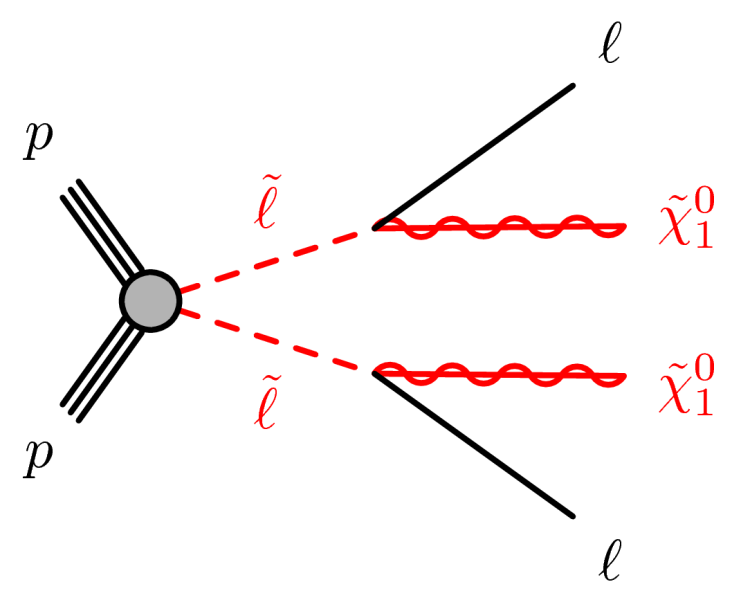
\includegraphics[width = 0.4\textwidth]{Figures/FeynmanDiagrams/SlepSlepFeynman.png}
    \caption{Direct slepton production $pp \rightarrow \tilde{l}^+ \tilde{l}^- \rightarrow l^+l^- + \tilde{\chi}_1^0 \tilde{\chi}_1^0$.}
    \label{fig:SlepSlepFeynman}
\end{figure}

In figure \ref{fig:SlepSnuFeynman} and \ref{fig:WWFeynman} we can see the chargino production with  slepton/sneutrino-mediated-decays and with W-boson-mediated-decays. Charginos are a mixture of the sparticles wino and the charged higgsino. These processes have the same final state as direct slepton production, but here the neutrinos are also a part of the MET, since we can't actually detect them in the detector. 
\begin{figure}[H]
    \centering
    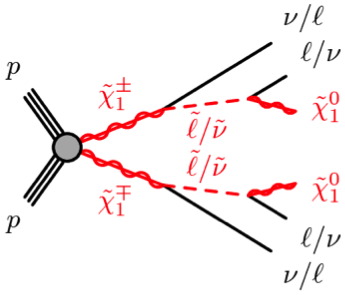
\includegraphics[width = 0.4\textwidth]{Figures/FeynmanDiagrams/SlepSnuFeynman.png}
    \caption{Chargino production with slepton/sneutrino-mediated-decays $pp \rightarrow \tilde{\chi}_1^+ \tilde{\chi}_1^- \rightarrow \tilde{l}^+ \tilde{l}^- /\tilde{\nu} \tilde{\nu} \rightarrow l^+l^- + \nu \Bar{\nu} + \tilde{\chi}_1^0 \tilde{\chi}_1^0$.}
    \label{fig:SlepSnuFeynman}
\end{figure}

\begin{figure}[H]
    \centering
    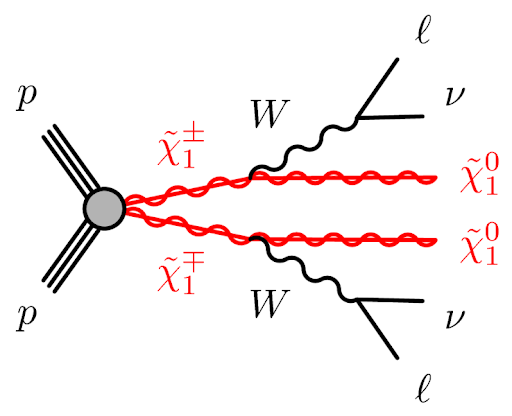
\includegraphics[width = 0.4\textwidth]{Figures/FeynmanDiagrams/WWFeynman.png}
    \caption{Chargino production with W-boson-mediated-decays $pp \rightarrow \tilde{\chi}_1^+ \tilde{\chi}_1^- \rightarrow W^+ W^- \rightarrow l^+l^- + \nu \Bar{\nu} + \tilde{\chi}_1^0 \tilde{\chi}_1^0$.}
    \label{fig:WWFeynman}
\end{figure}

The DM process we are looking at in this thesis is the mono-Z process shown in figure \ref{fig:monoZFeynman2}. Here we have a mediator V which decays into the DM particles $\chi$ and a W/Z that decays into two leptons. This gives us the same final state as we had for the SUSY processes.  

\begin{figure}[H]
    \centering
    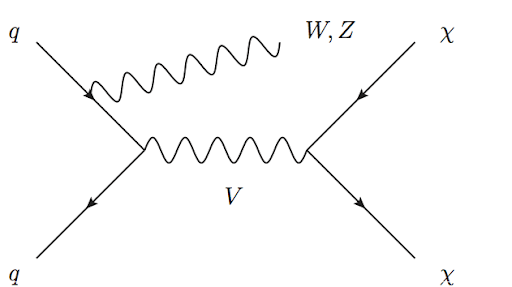
\includegraphics[width = 0.4\textwidth]{Figures/FeynmanDiagrams/monoZFeynman2.png}
    \caption{Mono-Z process $pp \rightarrow Z + MET \rightarrow l^+ l^- + MET$.}
    \label{fig:monoZFeynman2}
\end{figure}


\section{MC simulated events}

The data taken into consideration is from the ATLAS experiment at LHC between 2015-2018 (Run 2), further explained in chapter \ref{sec:LHCandATLAS}. But, we are also looking at some MC simulated background and signal which will be explained in this section. The explanations are taken from the publications from ATLAS, namely \cite{sleptonexclusion} for the SUSY signals and \cite{monoZexclusion} for the mono-Z signal. We present an overview of what signal samples that are used in table \ref{tab:directslepLOW} - \ref{tab:MonoZHigh} in section \ref{sec:sigsamptab}. 

The SUSY signal samples were generated from leading-order (LO) matrix elements with up to two extra partons using \textsc{MadGraph5\_aMC@NLO 2.6.1} \cite{48} interfaced to \textsc{Pythia 8.186} \cite{49}, with the A14 tune \cite{50}, for the modelling of the SUSY decay chain, parton showering, hadronisation and the description of the underlying event. Parton luminosities were provided by the NNPDF2.3LO PDF set \cite{51}. Jet–parton matching was performed following the CKKW-L prescription \cite{52}, with a matching scale set to one quarter of the mass of the pair-produced SUSY particles. Signal cross-sections were calculated to next-to-leading order (NLO) in $\alpha_s$ adding the resummation of soft gluon emission at next-to-leading-logarithm accuracy(NLO+NLL) \cite{53,54,55,56,57,58,59}. The nominal cross-sections and their uncertainties were taken from an envelope of cross-section predictions using different PDF sets and factorisation and renormalisation scales, as described in Ref. \cite{60}. 


To study the invisible Higgs boson decays, Monte Carlo events are produced for the SM ZH process with a subsequent Z boson decay into a dilepton pair and the H$\rightarrow$ZZ$\rightarrow \nu \nu \nu \nu$ decay (ZH$\rightarrow ll$+inv). The ZH signal processes from both the quark–antiquark (qqZH) and gluon–gluon (ggZH) initial states are modelled with \textsc{Powheg-Box v2} \cite{49Z, 50Z} using the CT10 \cite{51Z} parton distribution function (PDF) and interfaced to \textsc{Pythia8.186} \cite{52Z} for parton showering. The kinematic distributions of ZH$\rightarrow ll$ +inv events are described at next-to-leading-order (NLO) in QCD. Additionally, for the qqZH process, the MINLO \cite{53Z} method is applied to improve the gluon resummation calculation, and the $p_T^Z$ distribution is corrected to NLO electroweak (EW) accuracy with a reweighting approach detailed in Ref. \cite{3Z}. The SM ZH production cross-section is computed with next-to-next-to-leading-order (NNLO) QCD and NLO EW precision and found to be 884 fb \cite{3Z} with $m_H = 125$ GeV at 13 TeV. The DM signal is modelled with the leading-order \textsc{MadGraph5\_aMC@NLO} matrix element \cite{54Z} using NNPDF3.0 \cite{55Z} and showered with Pythia8.186. DM signal events with an axial-vector mediator and fermionic WIMPs are produced for different $m_{med}$ and $m_\chi$, both in a range from 10 to 1000 GeV.  As recommended in Ref. \cite{44Z}, the DM events are generated by choosing $g_q = 0.25$, $g_\chi = 1$, and a minimal mediator width. The AZNLO \cite{56Z} and A14 \cite{57Z} parameter sets are used to tune the \textsc{Pythia8.186} parton-shower for the simulation of the ZH $\rightarrow ll$+inv and DM signals, respectively.


The different backgrounds that we are considering are diboson, triboson, $t\Bar{t}$, single top, other top events ($t\Bar{t}$ events with a pair of leptons or boson(s)), Higgs, Drell-Yan, Z+jets and W+jets. The MC samples are simulated using different generators that are listed up in table \ref{tab:bkg_samples}. The goal is to separate these backgrounds from the signals we are looking at, which consist in the four different processes that we looked at earlier in this chapter. 

\begin{table}[H]
    \centering
    \begin{tabular}{l l l l} \toprule
        \textbf{Background sample} & \textbf{Generator} & \textbf{Parton shower} & \textbf{Normalisation}\\
        \midrule
        \midrule
        Diboson & \textsc{Sherpa2.2.2}\cite{sherpa2_1, sherpa1_2, sherpa1_3} & \textsc{Sherpa2.2.2} & NLO \cite{NLO}\\
        Triboson & \textsc{Sherpa2.2.2} & \textsc{Sherpa2.2.2} & NLO \\
        Z+jets & \textsc{Sherpa2.2.1} \cite{sherpa1_1, sherpa1_2, sherpa1_3} & \textsc{Sherpa2.2.1} & NNLO \cite{NNLO}\\
        W+jets & \textsc{Powheg-Box v2}\cite{49Z, 50Z} & \textsc{Pythia8.186} \cite{49} & NLO\\
        Drell-Yan & \textsc{Sherpa2.2.1} & \textsc{Sherpa2.2.1} & NNLO\\
        $t\Bar{t}$ & \textsc{Powheg-Box v2} & \textsc{Pythia8.186} & NNLO\\
        Single top & \textsc{Powheg-Box v2} & \textsc{Pythia8.186} & NLO\\
        topOther & \textsc{MG5\_aMC@NLO} \cite{48} & \textsc{Pythia8.186} & NLO\\
        Higgs & \textsc{Powheg-Box v2} & \textsc{Pyhtia8.186} & NLO\\
        \bottomrule
    \end{tabular}
    \caption{An overview of the different generators used to simulate the MC background samples.}
    \label{tab:bkg_samples}
\end{table}


Before we move on to how we perform the analysis, we also need to know how we are going to know that we see SUSY and DM particles in the detector. Since they never have been discovered, we have to lean on some hypotheses on how this is happening. As for all events in the detector, we have to reconstruct the events using their decays. The supersymmetric particles are expected to decay into cascades that will contain a LSP which will interact very weakly with the detector material which again will result in a big measured MET in the detector. The rest of the cascade will result in a final state with with leptons and/or jets. Together with the MET this gives us the final state we are looking for. For the mono-Z process we can measure the MET from the DM particles decayed from the unknown hypothetical mediator particle. Together with the leptons we get from the decay of the Z-boson, this gives us the same final state as for the SUSY processes.




































\begin{comment}

\begin{itemize}
    \item Bruker noe som eksisterer
    \item Tradisjonell måte ting har blitt gjort på
    \item begrenset av menneskets forståelse av prosessen vi ser på
    \item vi må bestemme alle kuttene som blir gjort
    \item Du må vite hva du skal se etter for å gjøre dette, altså trenger en teori/hypotese
    \item Tenk overgang til ML
    \item Valg må være begrunnet 
    \item Massesplitting. Cut and count er svak på lav massesplitting. Dette gjør ML bedre
\end{itemize}
\end{comment}








\section{The standard way: cut and count}
\label{sec:candc}

The first part of the analysis done in this thesis is a traditional cut and count analysis. \textit{Cut and count} is probably the most known method used in particle physics and has proved to be very useful in the discoveries we have done so far. Since the data become more and more massive and the processes we are looking at more and more complicated, we also need to develop further the way we perform the analysis. In this thesis, we are mainly going to focus on machine learning algorithms. Therefore we have not done much with this standard way to analyze and have based the cut and count on already published analyses from ATLAS \cite{sleptonexclusion, monoZexclusion}. 

In cut and count, we select events sensitive to new physics, i.e., we remove events which are not interesting for the signal process we consider. After applying several cuts, the selection of events we are left with form the so-called \textit{signal region}. We then see whether the expected signal is significantly separated from the expected Standard Model (SM) background in this region. We can calculate an expected significance $Z$, which will be explained in section \ref{sec:significance} later in the thesis, to check if we can expect to claim a discovery in this region if a particular signal model turns out to be realized in nature. If we are lucky and have cut away enough background and kept sufficient signal, we can check if the observed events in data are compatible with the signal+background hypothesis or if they match the background-only hypothesis (i.e. no signal) instead. Let us consider the case where the data differ from the background and tends to follow the signal: we know that there is most likely something interesting in this region.

Of course, there are advantages and disadvantages with every method, and this is also the case for cut and count. In cut and count, we need a theory or hypothesis as a reference to know what kind of signals we should look for. It is therefore unfortunately limited by the human understanding of what we are looking at. The lack of human understanding is where Machine Learning (ML) comes to help. The ML methods help us separate the signal from the background. This is further explained in the following chapters, where we will look at what the different ML methods do.






\section{Reproducing the ATLAS publications}
The first part of this analysis was done by cut and count and the goal was to reproduce the results from publications done by ATLAS \cite{sleptonexclusion, monoZexclusion}. Here we will compare our results to the official results from the ATLAS experiment, and hopefully achieve a good agreement between the two.

Since the goal is to reproduce the results, we implement more or less the same analysis procedure as described in the publications. The cuts done for the SUSY processes are listed in table \ref{tab:cutsSUSY} and for the mono-Z process in table \ref{tab:cutsDM}, where both tables are taken from the publications \cite{sleptonexclusion, monoZexclusion}. All the kinematic variables we cut on are presented in chapter \ref{sec:LHCandATLAS}. The first cut we do for both processes is to demand exactly two leptons with opposite signs in the final state.


\begin{table}[H]
    \centering
    \begin{tabular}{l l}\toprule
    \textbf{Variables} & \textbf{Cuts}\\
    \midrule
    \midrule
    Two leptons & Same flavor (SF) and opposite sign (OS)\\
    $n_{\text{non-b-tagged jets}}$     & 0 \\
    $m_{ll}$ [GeV]     & 121.2\\
    $E_T^{miss}$ [GeV] & $>$ 110 \\
    $E_T^{miss}$ significance & $>$ 10\\
    $n_{\text{b-tagged jets}}$ & 0\\
    $m_{T2}$ [GeV] & 160\\
    \bottomrule
    \end{tabular}
    \caption{Cuts added in the cut and count analysis taken from the publication for the SUSY processes \cite{sleptonexclusion}.}
    \label{tab:cutsSUSY}
\end{table}

For the SUSY processes we have applied the cuts in table \ref{tab:cutsSUSY}, where we, in addition to having only two leptons with opposite sign in the final state, demand that they have to have the same flavor as well. Here we get the Z+jets as the dominating background as we can see in both figure \ref{fig:nJetSUSY} and table \ref{tab:cutflowSUSY}. Now we want to reduce all of the background, especially Z+jets, and we apply the next cut in table \ref{tab:cutsSUSY} which is demanding no jets. As we can see in figure \ref{fig:mllSUSY}, the Z+jets background is still the dominating background, but if we look at table \ref{tab:cutflowSUSY}, we can see that it is reduced a lot. The reason for Z+jets is still dominating is that the jet-cut reduced around the same percentage from all of the different backgrounds. 

\begin{figure}[H]
\centering
    \begin{subfigure}[t!]{0.49\textwidth}
        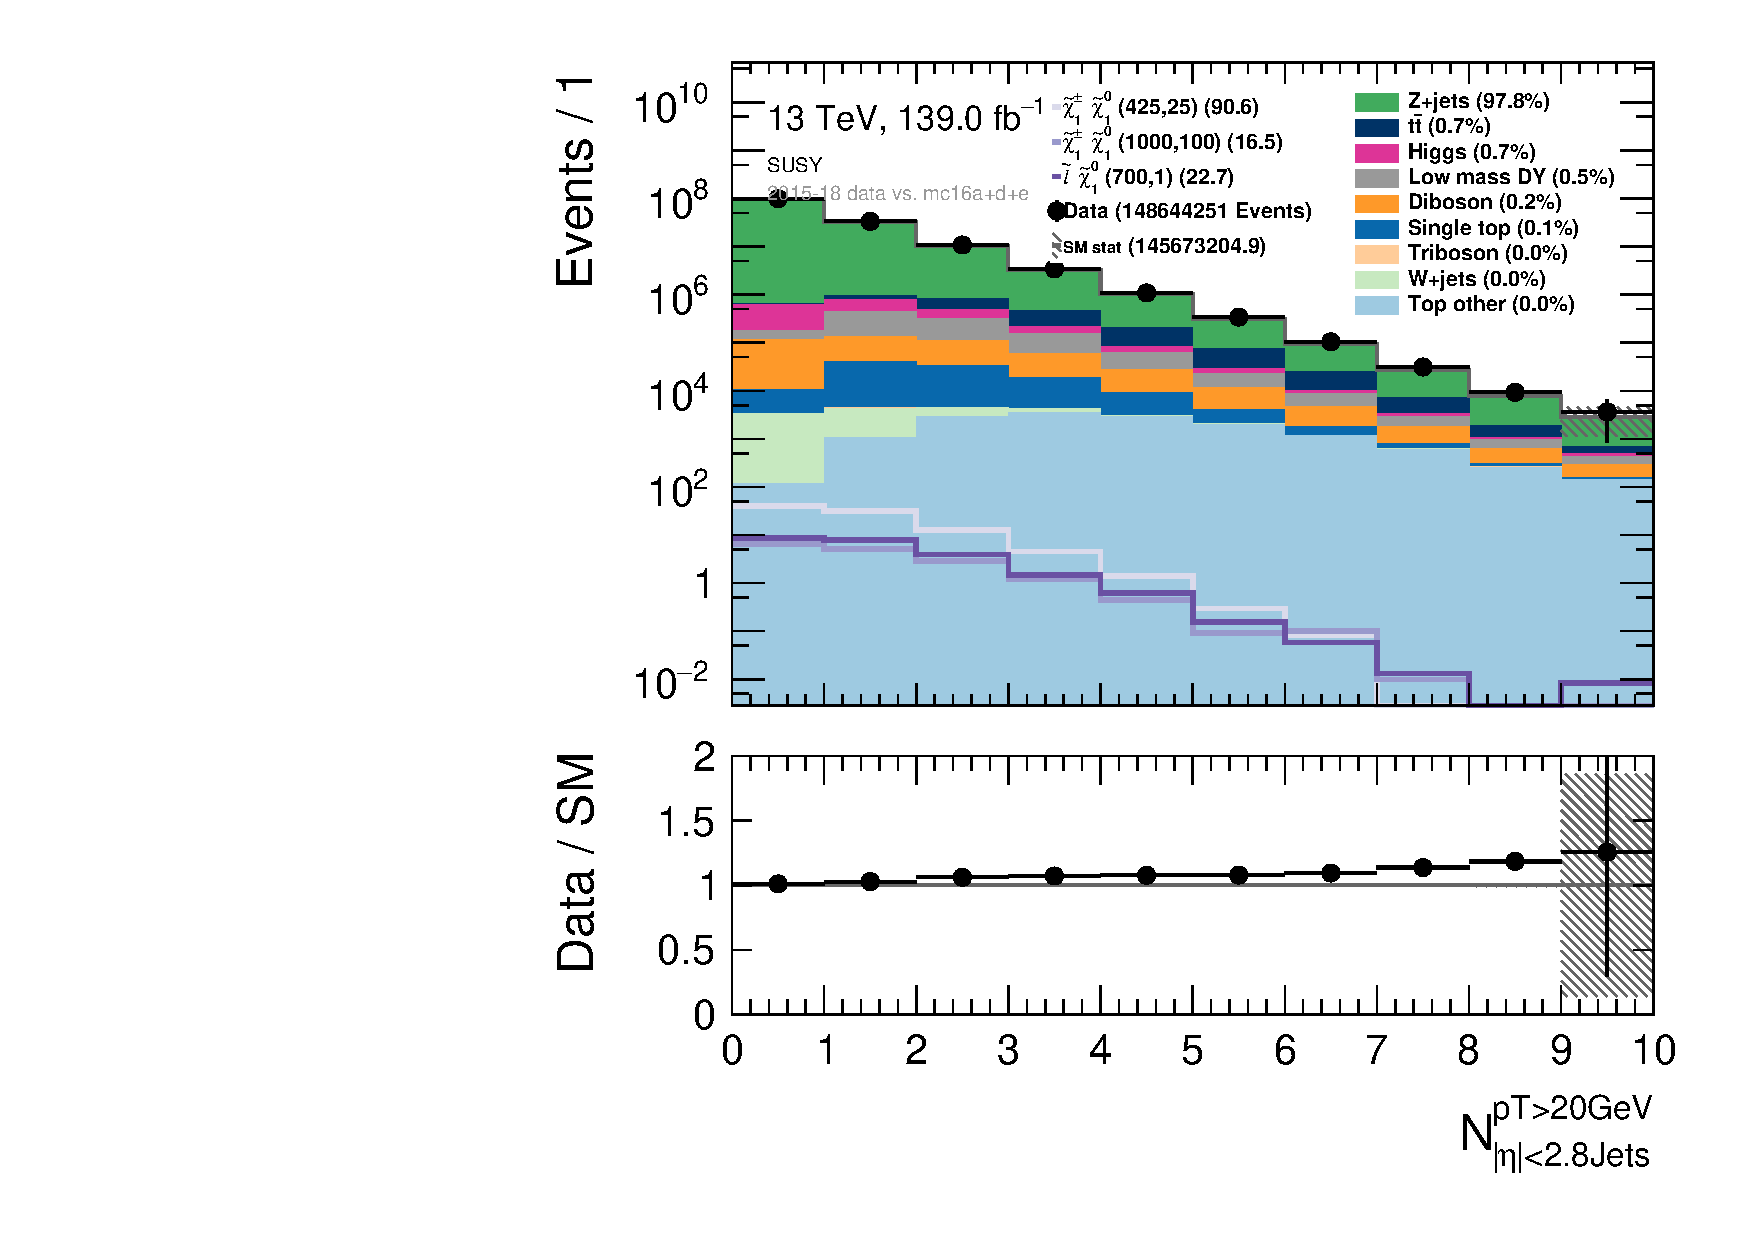
\includegraphics[width=\textwidth]{Figures/SUSYcuts/hist1d_nJet20_SUSY.pdf}
    \caption{Number of jets with a $p_T > 20$ GeV.}
    \label{fig:nJetSUSY}
    \end{subfigure}
    \begin{subfigure}[t!]{0.49\textwidth}
        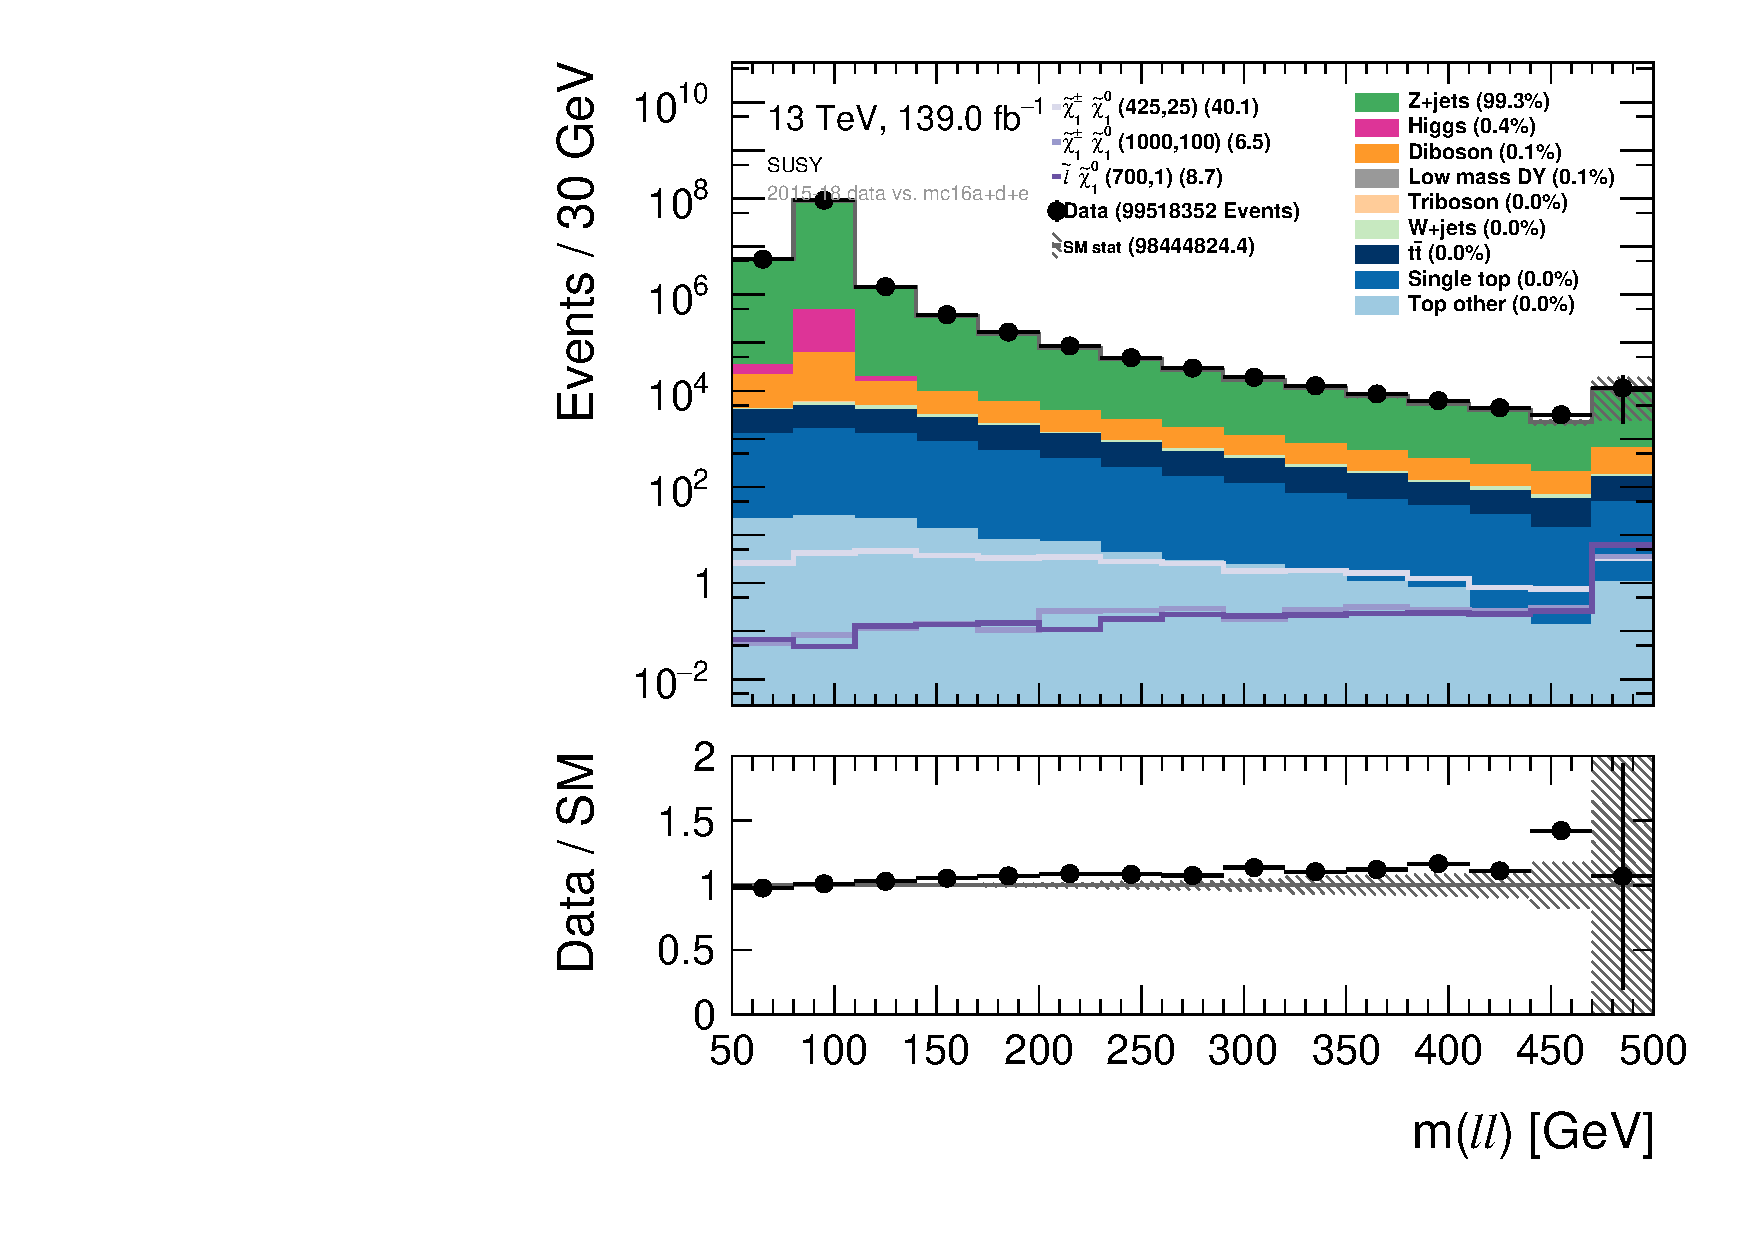
\includegraphics[width=\textwidth]{Figures/SUSYcuts/hist1d_mll_SUSY.pdf}
    \caption{The invariant mass of the two leptons.}
    \label{fig:mllSUSY}
    \end{subfigure}
    \caption{Plot of different distributions after applying the cuts on 2L, SF, OS and no jets.}
    \label{fig:stepsSUSY1}
\end{figure}


The next cut we have applied is on the invariant mass of the two leptons in the final state. The results are shown in figure \ref{fig:metSUSY} and as we can see, all of the background is reduced a lot. It is also done a cut requiring large missing transverse energy. This is done because it cuts away more background than signal, which entails obtaining a more significant separation between the signal and background. By applying this cut, we can see that the Z+jets are no longer the dominating background and the results are shown in figure \ref{fig:metSignSUSY} and table \ref{tab:cutflowSUSY}. 

\begin{figure}[H]
    \centering
    \begin{subfigure}[t!]{0.49\textwidth}
        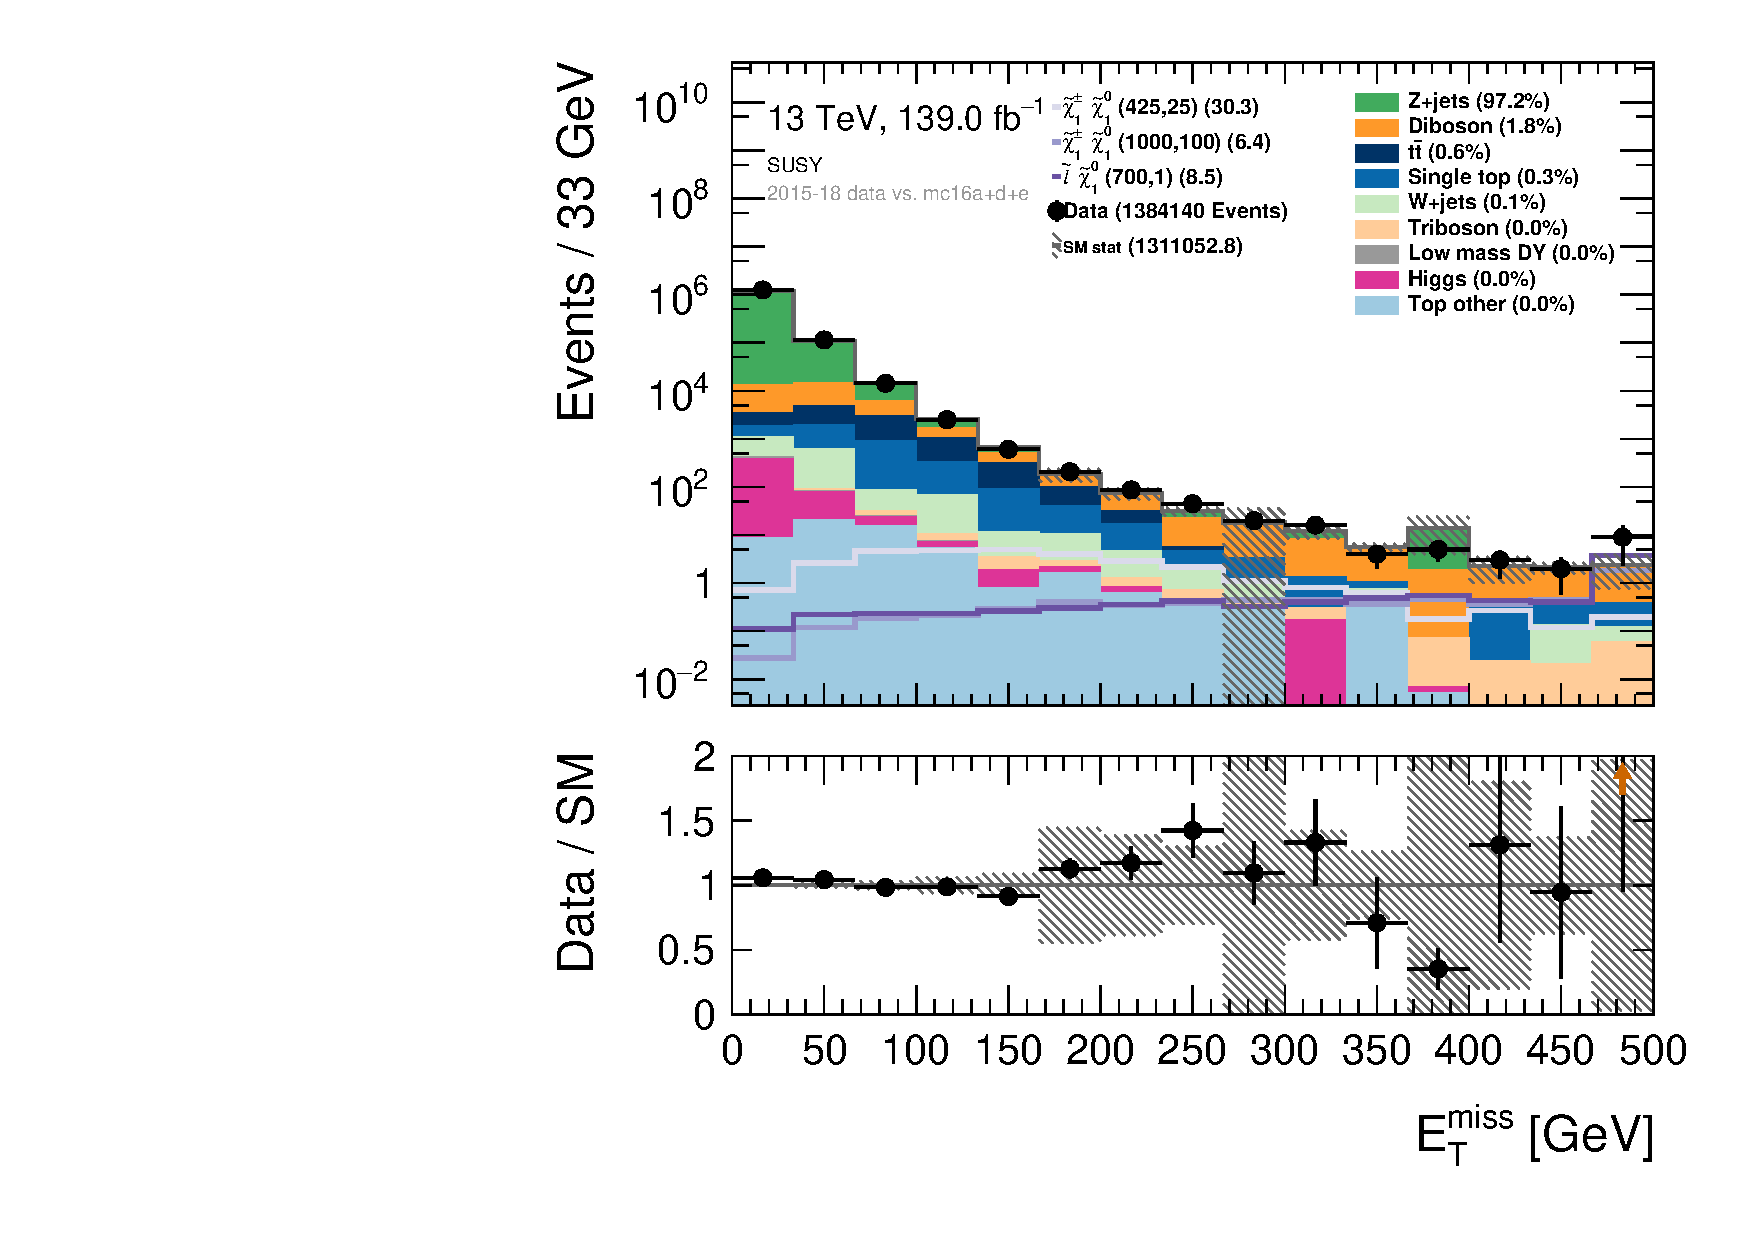
\includegraphics[width=\textwidth]{Figures/SUSYcuts/hist1d_met_Et_SUSY.pdf}
    \caption{Missing transverse energy.}
    \label{fig:metSUSY}
    \end{subfigure}
    \begin{subfigure}[t!]{0.49\textwidth}
        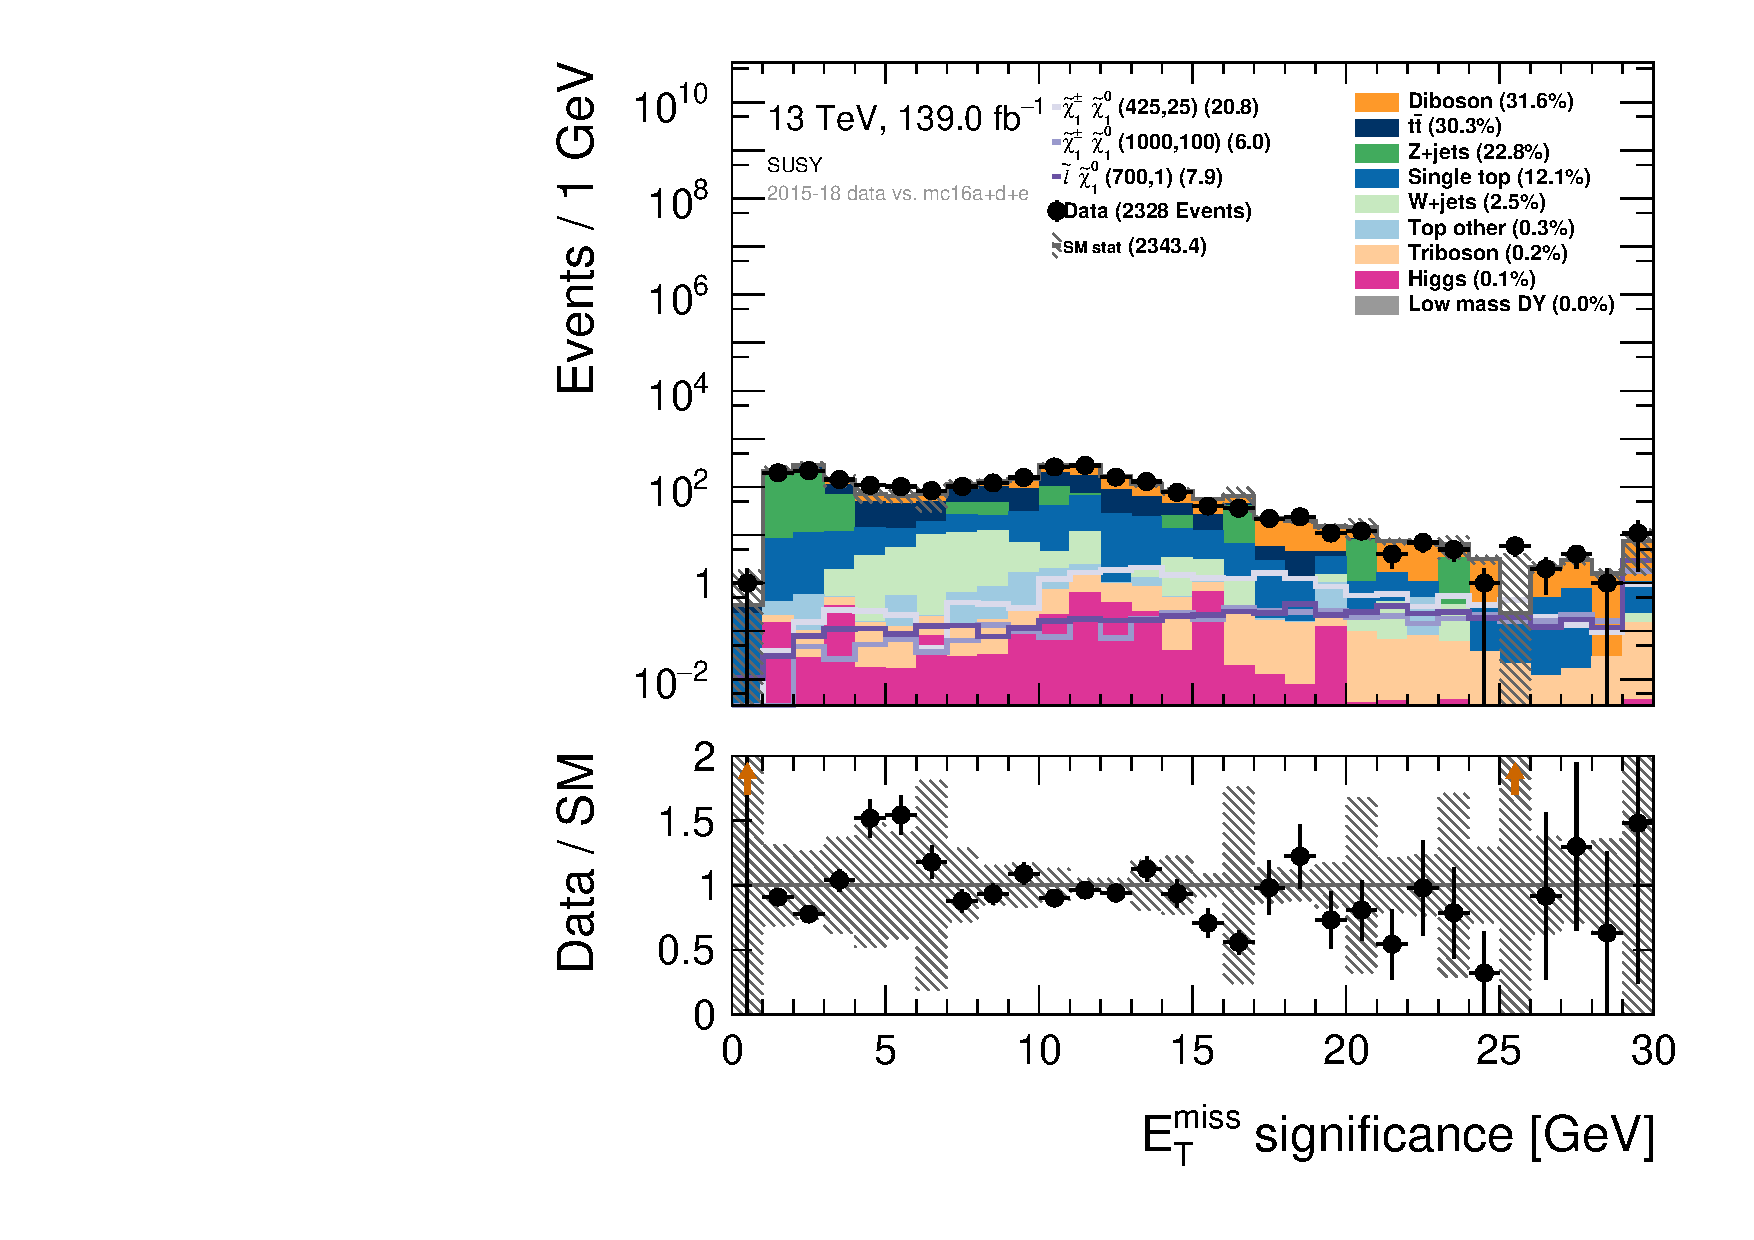
\includegraphics[width=\textwidth]{Figures/SUSYcuts/hist1d_met_Sign_SUSY.pdf}
    \caption{Missing transverse energy significance.}
    \label{fig:metSignSUSY}
    \end{subfigure}
    \caption{Plot of different distributions after applying the cuts on the invariant mass and MET.}
    \label{fig:stepsSUSY2}
\end{figure}


The last three cuts applied is a cut on the MET significance, b-tagged jets and $m_{T2}$. The results after applying the MET significance cut is shown in figure \ref{fig:bjetSUSY} and as we can see, the diboson is still the dominating background. The second last cut that was done is to demand events with non b-tagged jets which do not reduce anything because we already have demanded no jets at all. This we can see in figure \ref{fig:mt2SUSY} and table \ref{tab:cutflowSUSY}. The last cut that are applied for the SUSY processes are on the $m_{T2}$ variable. This is done to get rid of the rest of the $t\Bar{t}$ background and leave us more or less with only diboson. This is part of our final result and are shown in figure \ref{fig:cutandcountMONA} later in this section.

\begin{figure}[H]
    \centering
    \begin{subfigure}[t!]{0.49\textwidth}
        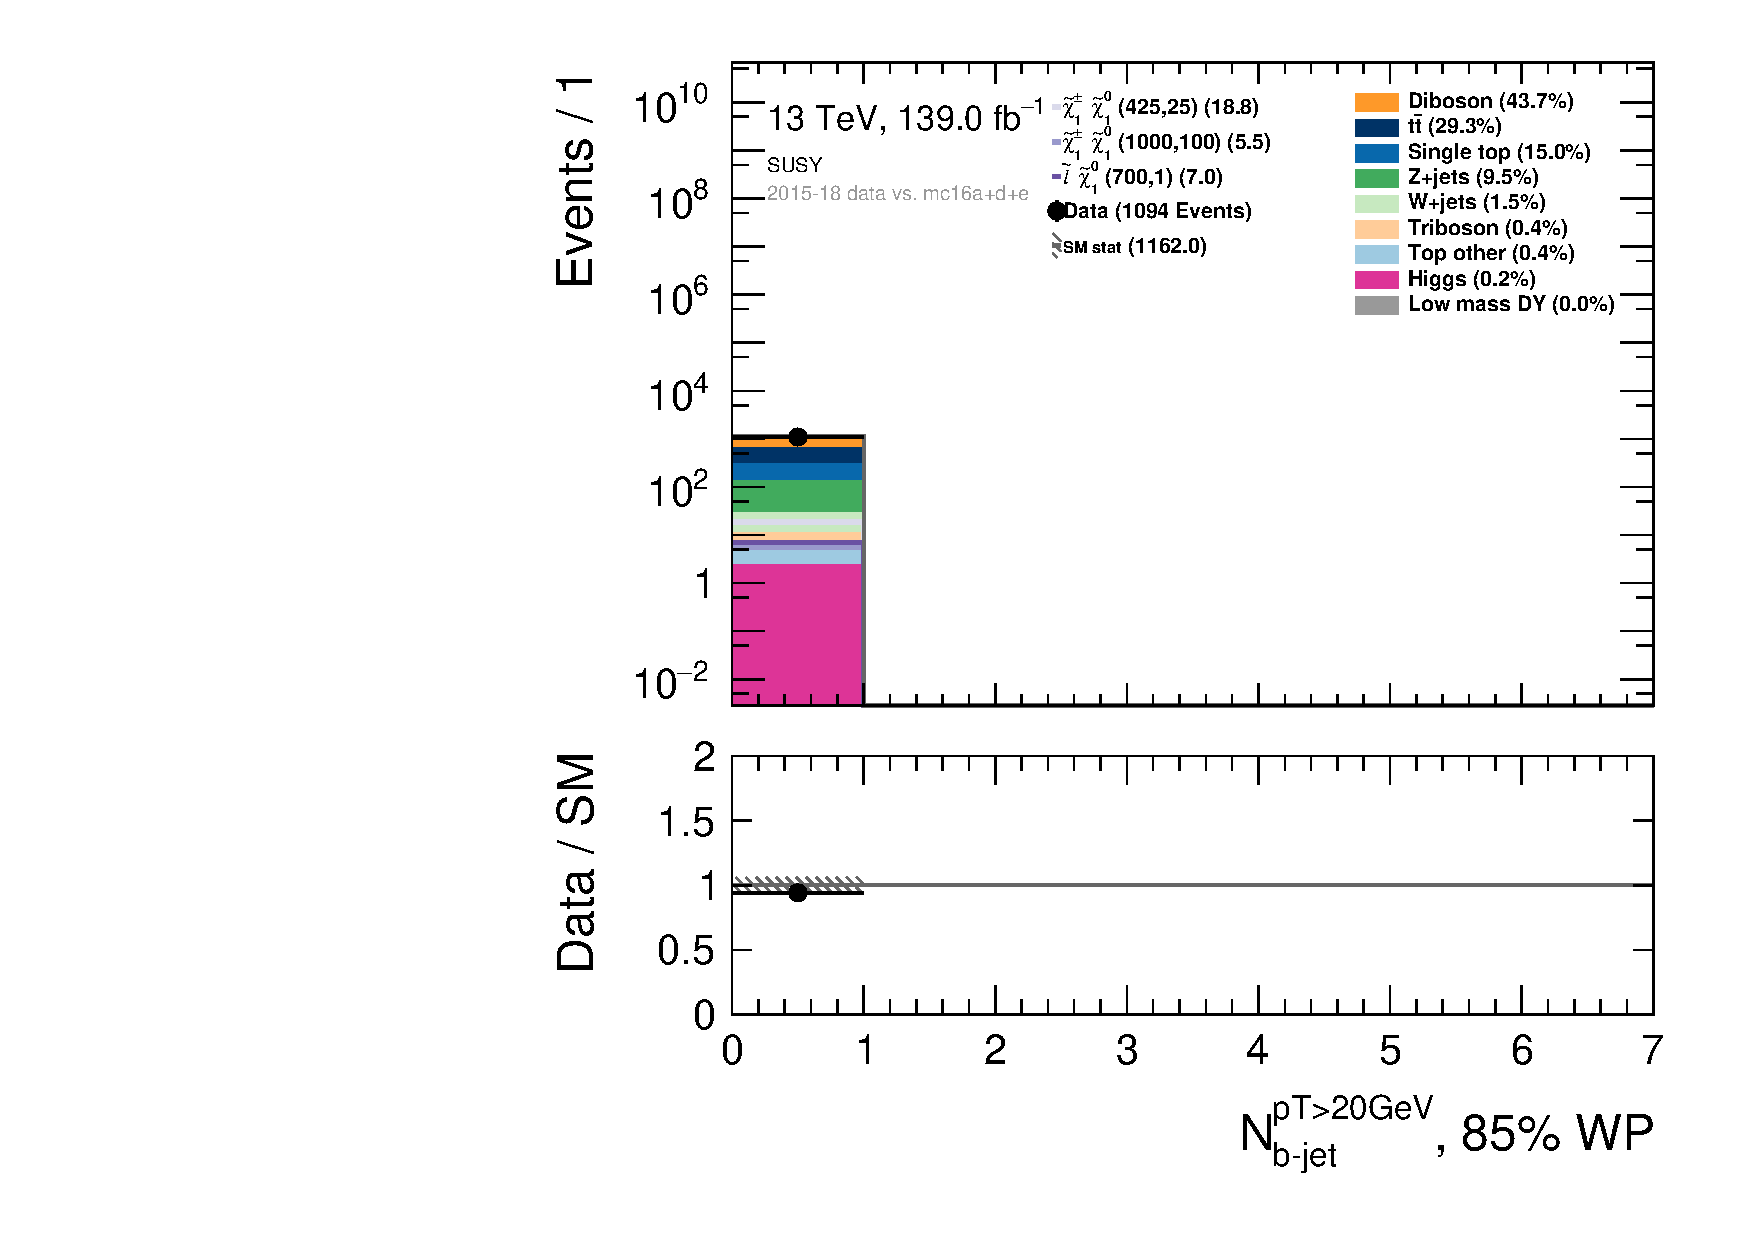
\includegraphics[width=\textwidth]{Figures/SUSYcuts/hist1d_nBJet20_MV2c10_FixedCutBEff_85_SUSY.pdf}
    \caption{Number of b-tagget jets.}
    \label{fig:bjetSUSY}
    \end{subfigure}
    \begin{subfigure}[t!]{0.49\textwidth}
        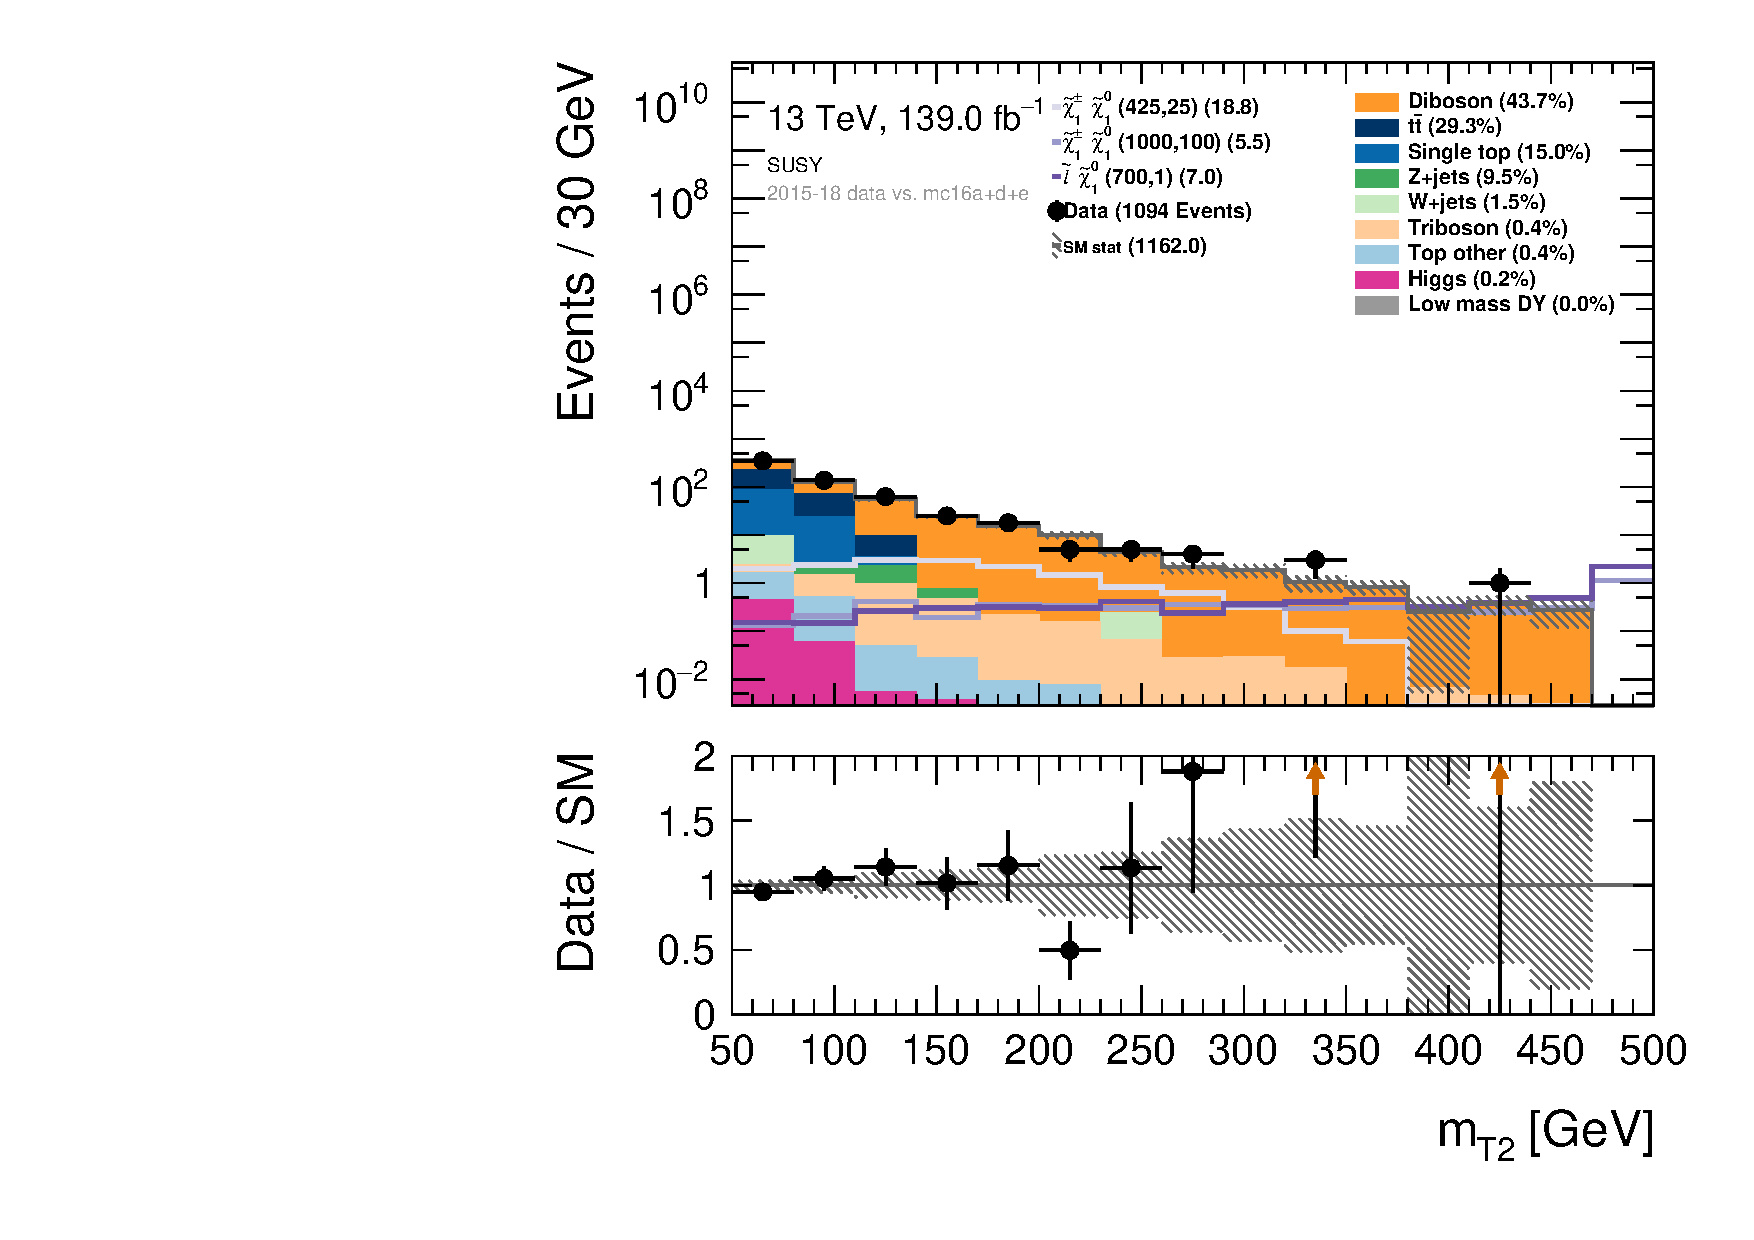
\includegraphics[width=\textwidth]{Figures/SUSYcuts/hist1d_mt2_SUSY.pdf}
    \caption{Stransverse mass.}
    \label{fig:mt2SUSY}
    \end{subfigure}
    \caption{Plot of different distributions after applying the cuts on MET significance and b-jets.}
    \label{fig:stepsSUSY3}
\end{figure}

As we can see in figure \ref{fig:stepsSUSY1}-\ref{fig:stepsSUSY3} and table \ref{tab:cutflowSUSY}, the signal have been reduced, but not as much as all of the background contributions. This implies that we have been able to get rid of the background without affecting the signal too much, which also was our goal by doing this. 

\begin{landscape}
\begin{table}[H]
    \centering
    %\rotatebox{90}{
    \begin{tabular}{l l l l l l l l}
    \toprule
    \textbf{Sample} & \textbf{OS+SF+2L} & \textbf{jet-veto} & $\mathbf{m_{ll}}$ & \textbf{MET} & \textbf{MET sign} & \textbf{b-jets} & $\mathbf{m_{T_2}}$\\
    \midrule
    \midrule
        Drell-Yan & 733055.427 & 64177.536 & 40.384 & 0.000 & 0.000 & 0.000 & 0.000 \\
        Higgs & 1055360.610 & 442535.035 & 451.966 & 3.222 & 2.411 & 2.411 & 0.005\\
        Single top & 96745.087 & 7383.056 & 3313.872 & 283.960 & 174.644 & 174.644 & 0.000\\
        $t\Bar{t}$ & 948716.615 & 16272.119 & 7648.974 & 710.246 & 340.903 & 340.903 & 0.000\\
        Z+jets & 142460122.600 & 97803688.386 & 1273912.476 & 533.182 & 109.925 & 109.925 & -0.004\\
        Top other & 14730.742 & 120.671 & 56.003 & 8.079 & 4.353 & 4.353 & 0.034\\
        W+jets & 8978.117 & 3252.185 & 1359.621 & 58.245 & 17.834 & 17.834 & 0.182\\
        Triboson & 345.791 & 65.545 & 25.860 & 5.757 & 4.633 & 4.633 & 0.653\\
        Diboson & 355149.910 & 107329.899 & 24243.651 & 740.741 & 507.329 & 507.329 & 42.588\\
        Data & 148644251.000 & 99518352.000 & 1384140.000 & 2328.000 & 1094.000 & 1094.000 & 40.000\\
        $(\Tilde{l}, \Tilde{\chi}_1^0) (700,1)$ & 22.710 & 8.692 & 8.519 & 7.873 & 6.987 & 6.987 & 6.062\\
        $(\Tilde{\chi}_1^\pm, \Tilde{\chi}_1^0) (1000, 100)$ & 16.475 & 6.546 & 6.355 & 5.997 & 5.468 & 5.468 & 4.347\\
        $(\Tilde{\chi}_1^\pm, \Tilde{\chi}_1^0) (425,25)$ & 90.581 & 40.109 & 30.305 & 20.816 & 18.756 & 18.756 & 6.692\\
    \bottomrule
    \end{tabular}
    %}
    \caption{A cut flow overview after applying the different cuts in table \ref{tab:cutsSUSY} with one signal sample from the three SUSY processes.}
    \label{tab:cutflowSUSY}
\end{table}
\end{landscape}




\begin{comment}


\newgeometry{twoside,inner=3cm,outer=2cm}
\begin{figure}[H]
%\begin{minipage}{2\textwidth}
%\begin{adjustwidth}{-3cm}{-3cm}
\centering
%\advance\leftskip-4cm 
%\advance\rightskip-4cm 
    \begin{subfigure}[t!]{0.49\textwidth}
        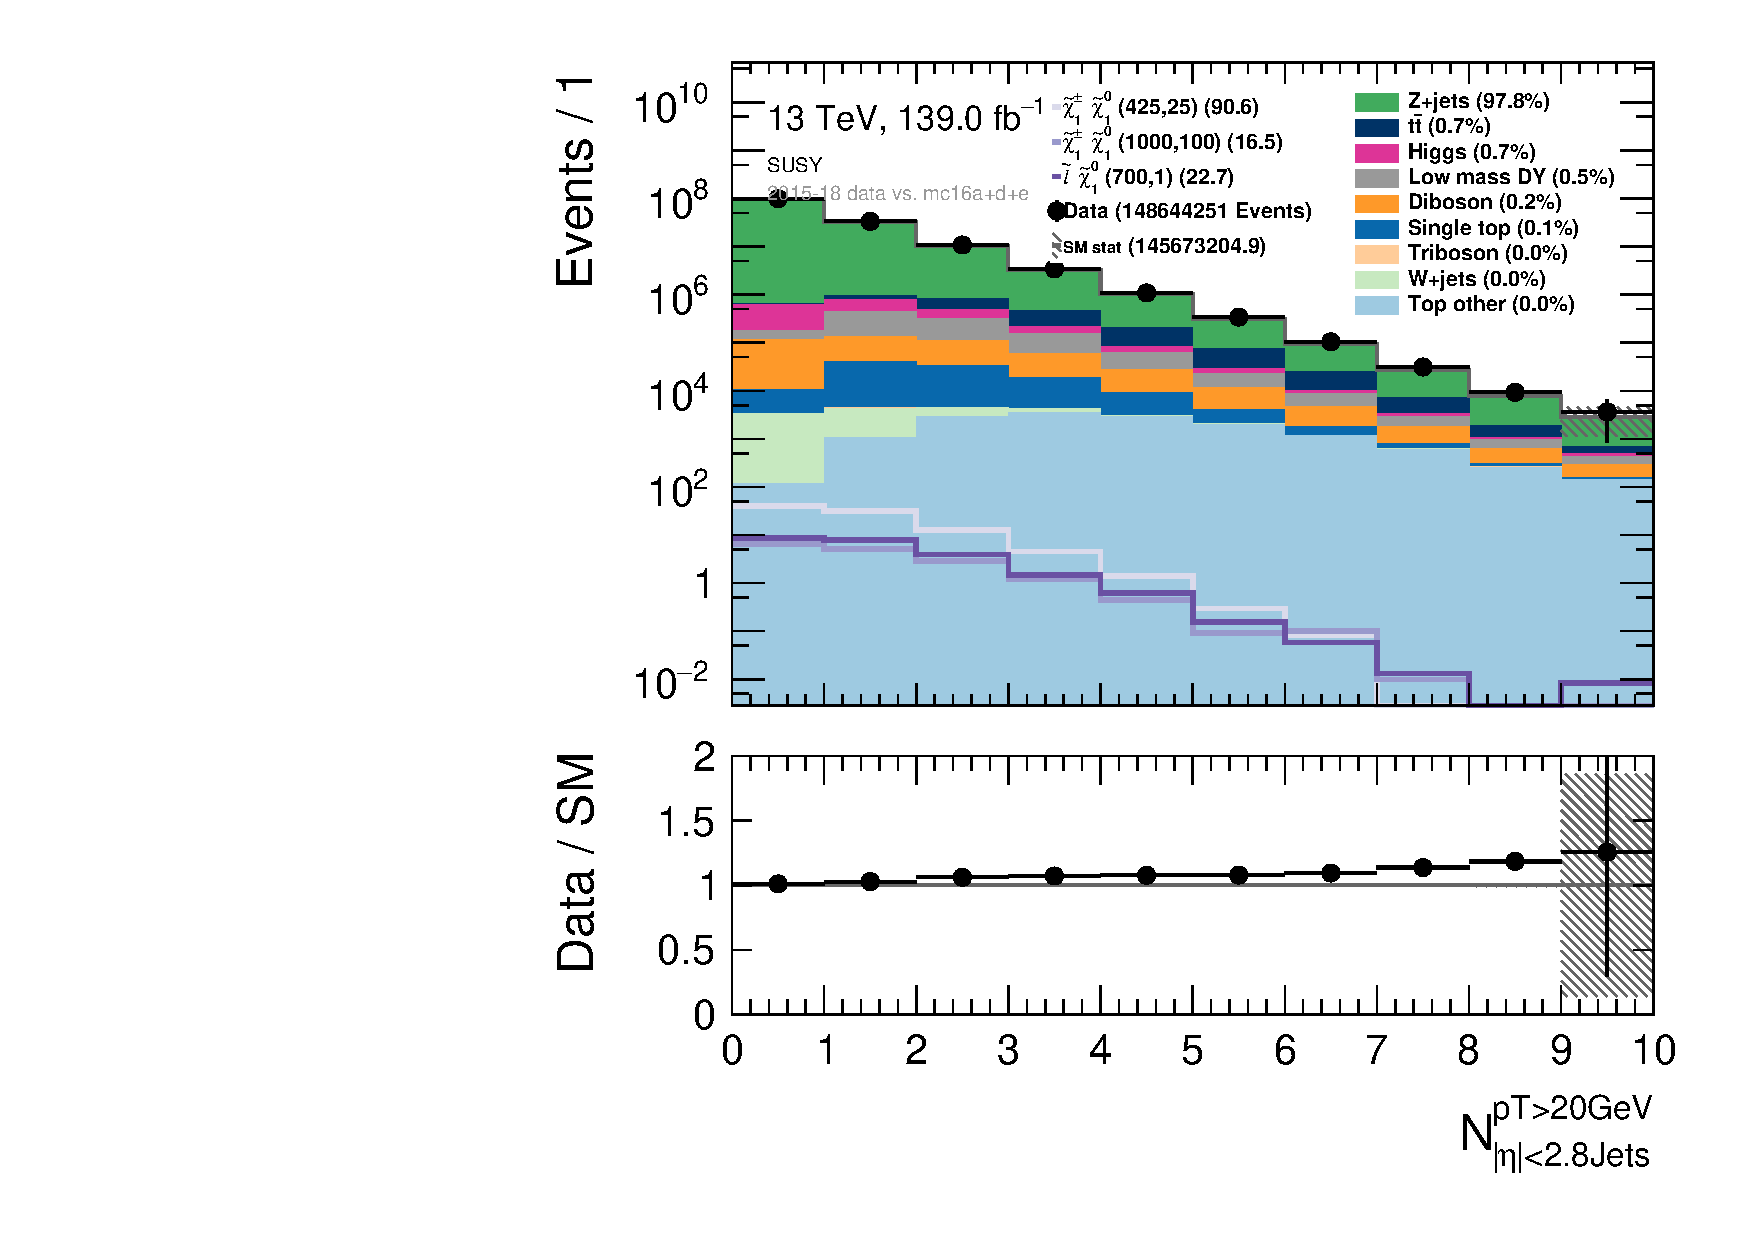
\includegraphics[width=\textwidth]{Figures/SUSYcuts/hist1d_nJet20_SUSY.pdf}
    \caption{Stransverse mass for direct slepton production.}
    \label{fig:my_label}
    \end{subfigure}
    \begin{subfigure}[t!]{0.49\textwidth}
        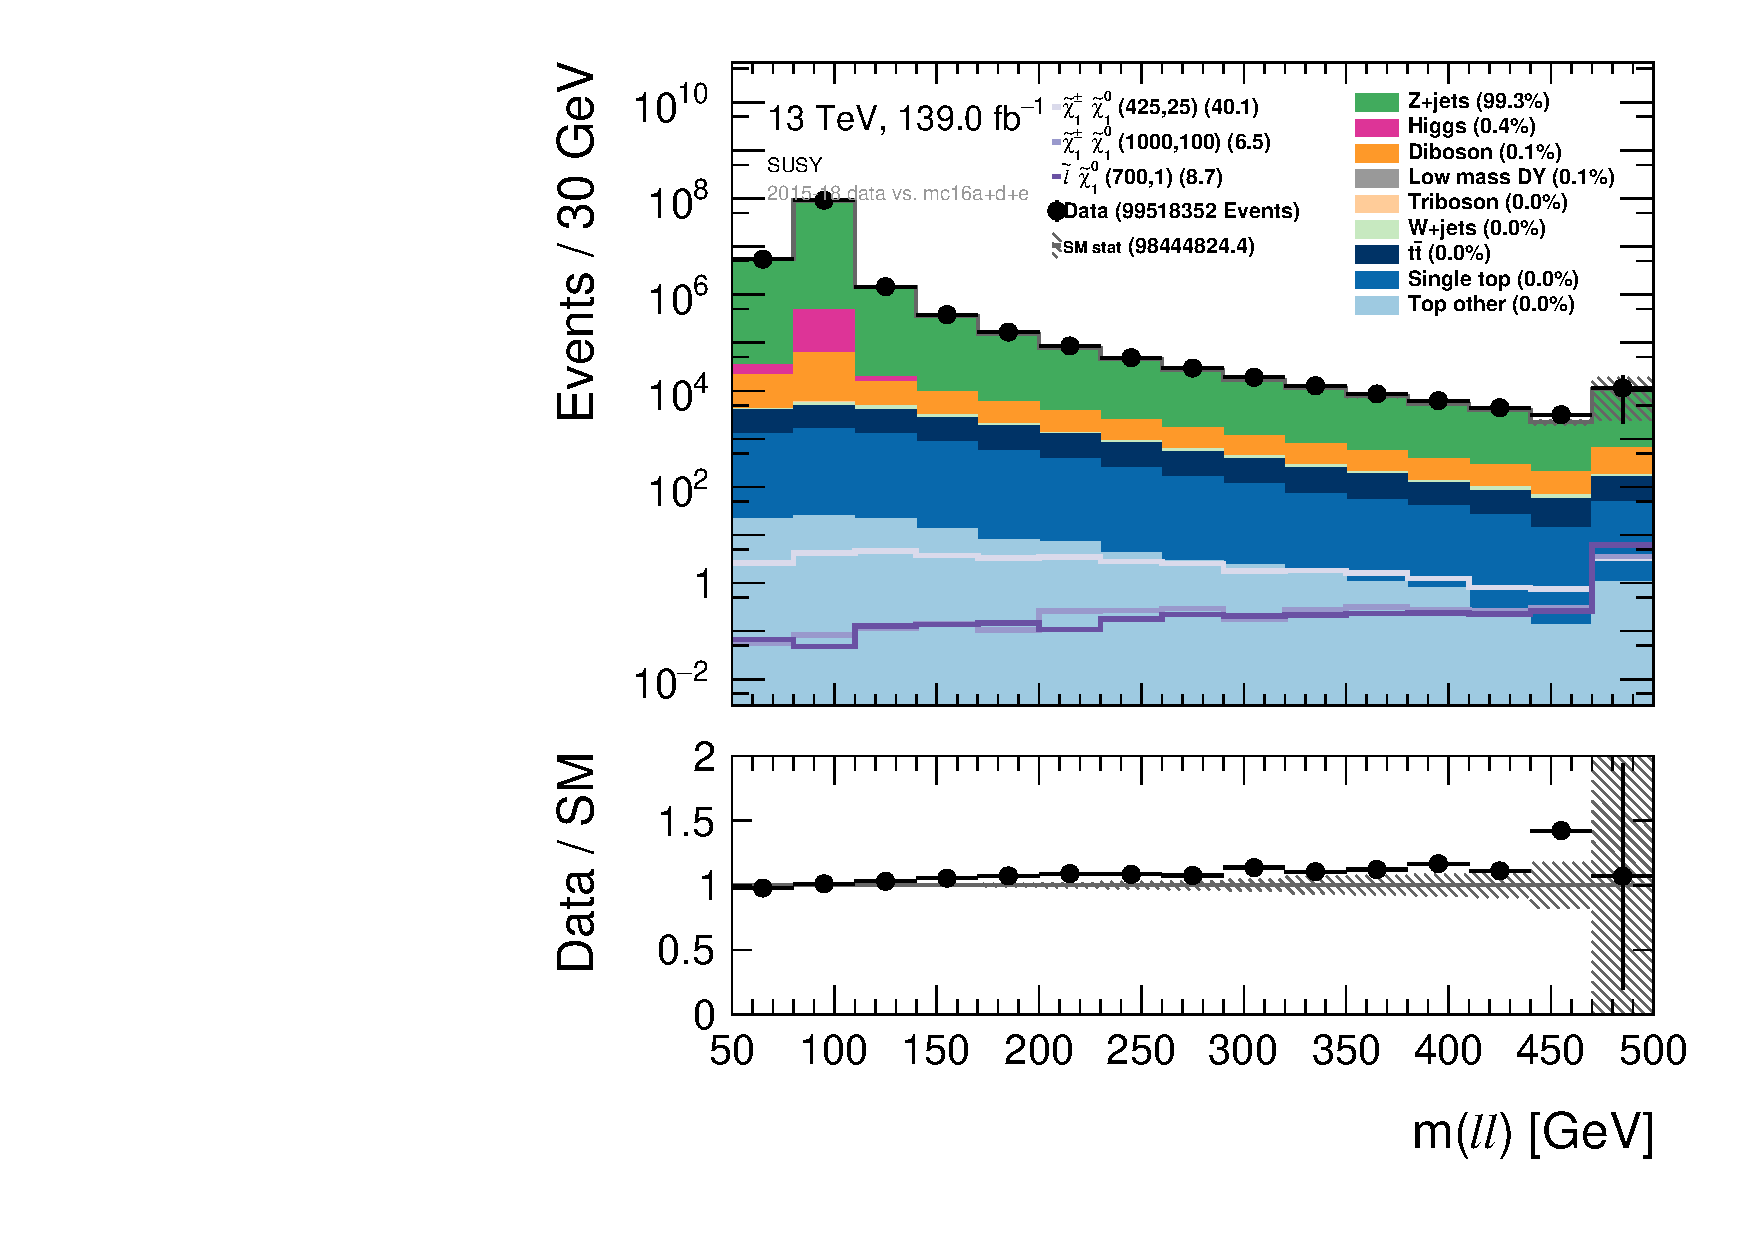
\includegraphics[width=\textwidth]{Figures/SUSYcuts/hist1d_mll_SUSY.pdf}
    \caption{Stransverse mass for chargino production via $\Tilde{l}/\Tilde{\nu}$.}
    \label{fig:my_label}
    \end{subfigure}
    \\
    \begin{subfigure}[t!]{0.49\textwidth}
        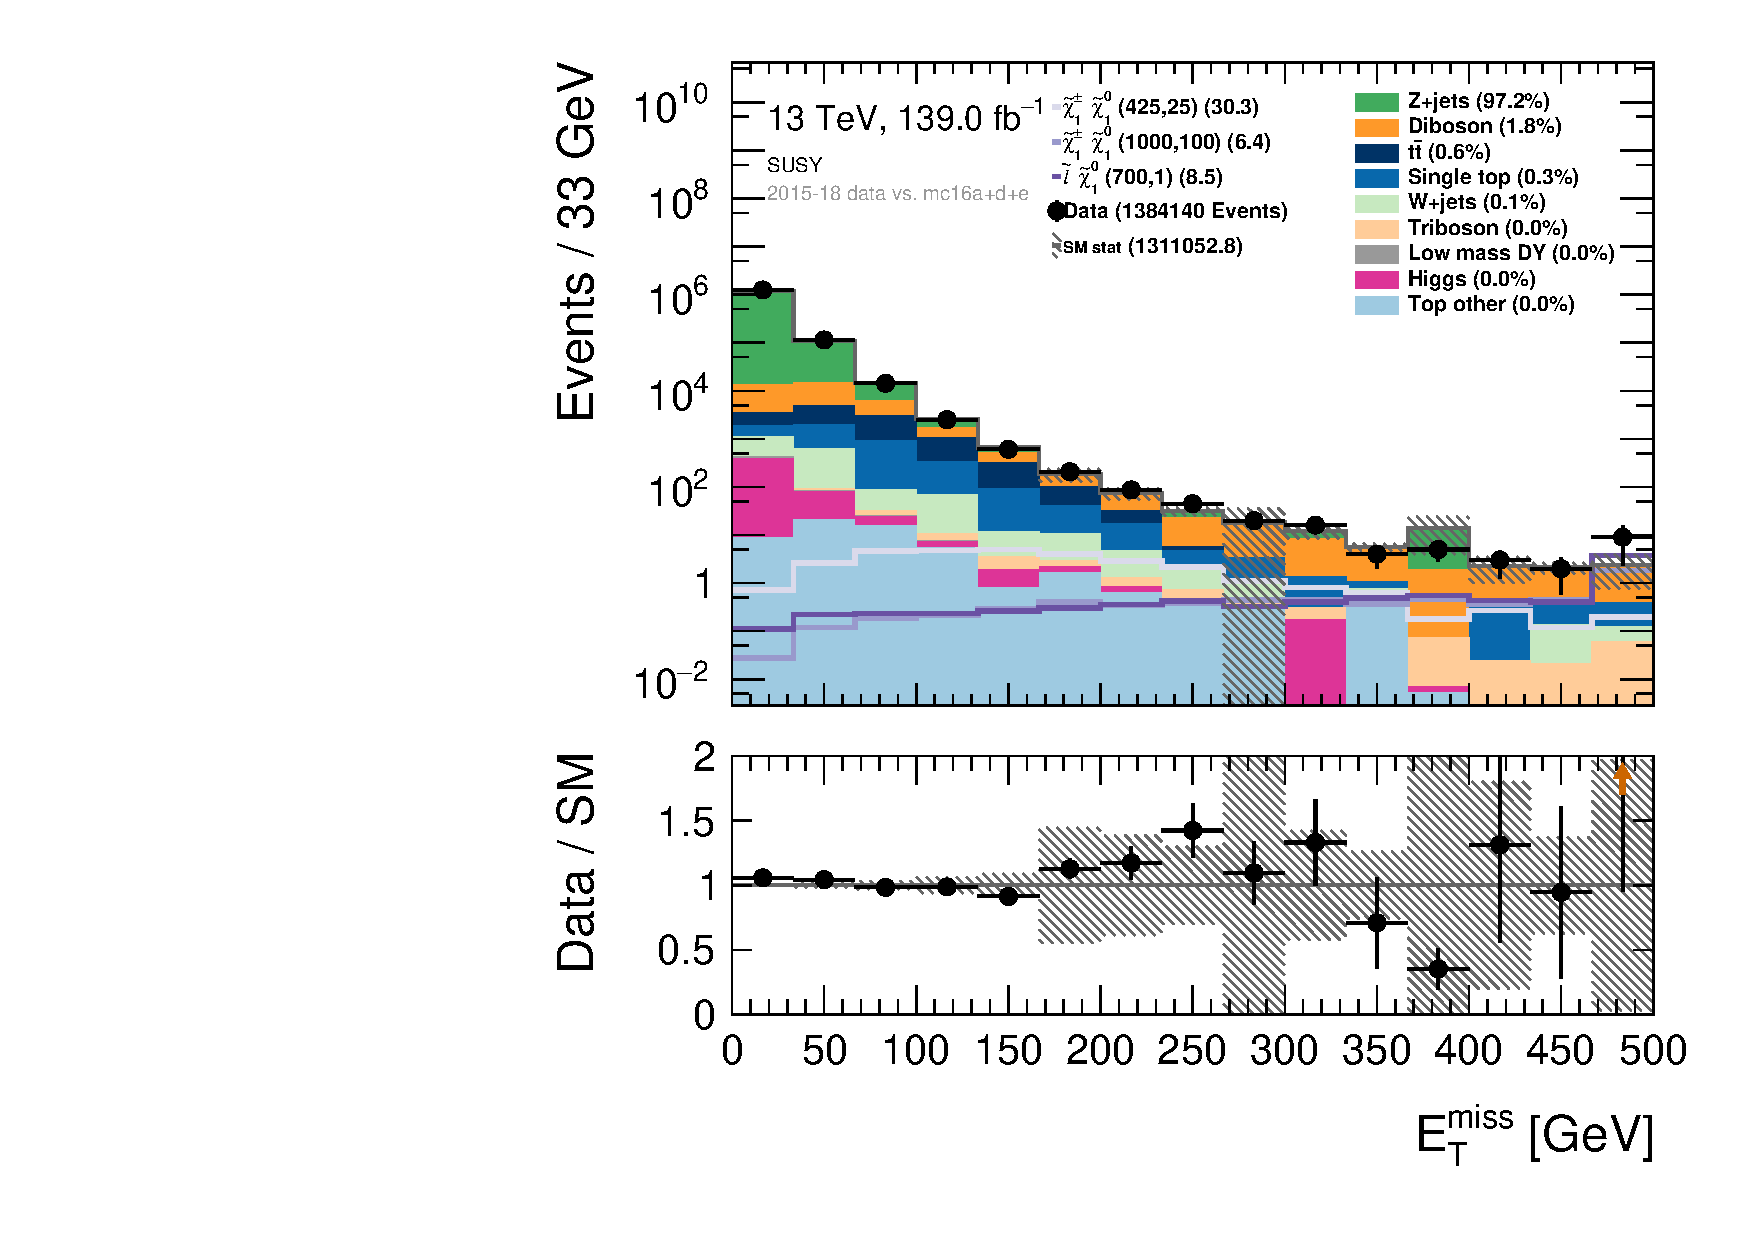
\includegraphics[width=\textwidth]{Figures/SUSYcuts/hist1d_met_Et_SUSY.pdf}
    \caption{Stransverse mass for chargino production via $W^\pm$.}
    \label{fig:my_label}
    \end{subfigure}
    \begin{subfigure}[t!]{0.49\textwidth}
        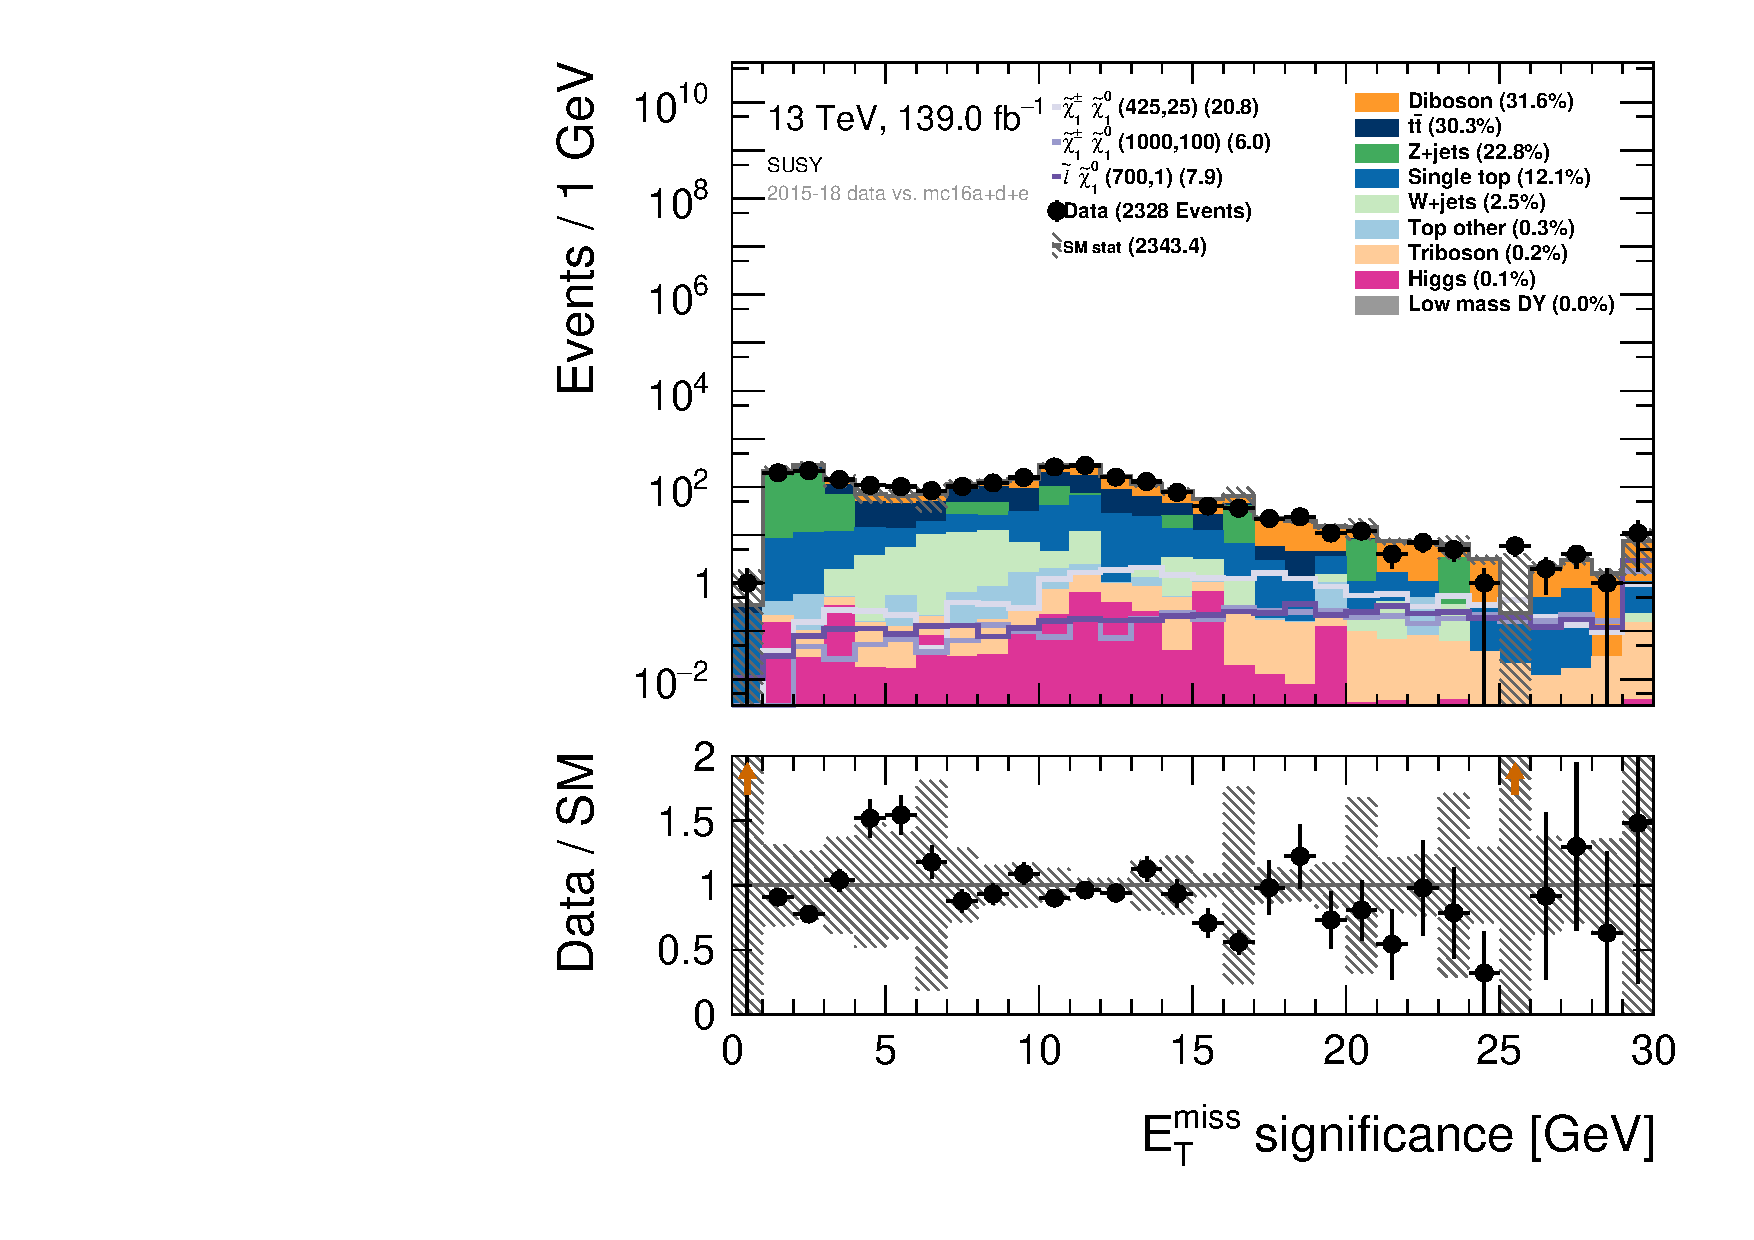
\includegraphics[width=\textwidth]{Figures/SUSYcuts/hist1d_met_Sign_SUSY.pdf}
    \caption{Missing transverse energy for mono-Z.}
    \label{fig:my_label}
    \end{subfigure}
    \\
    \begin{subfigure}[t!]{0.49\textwidth}
        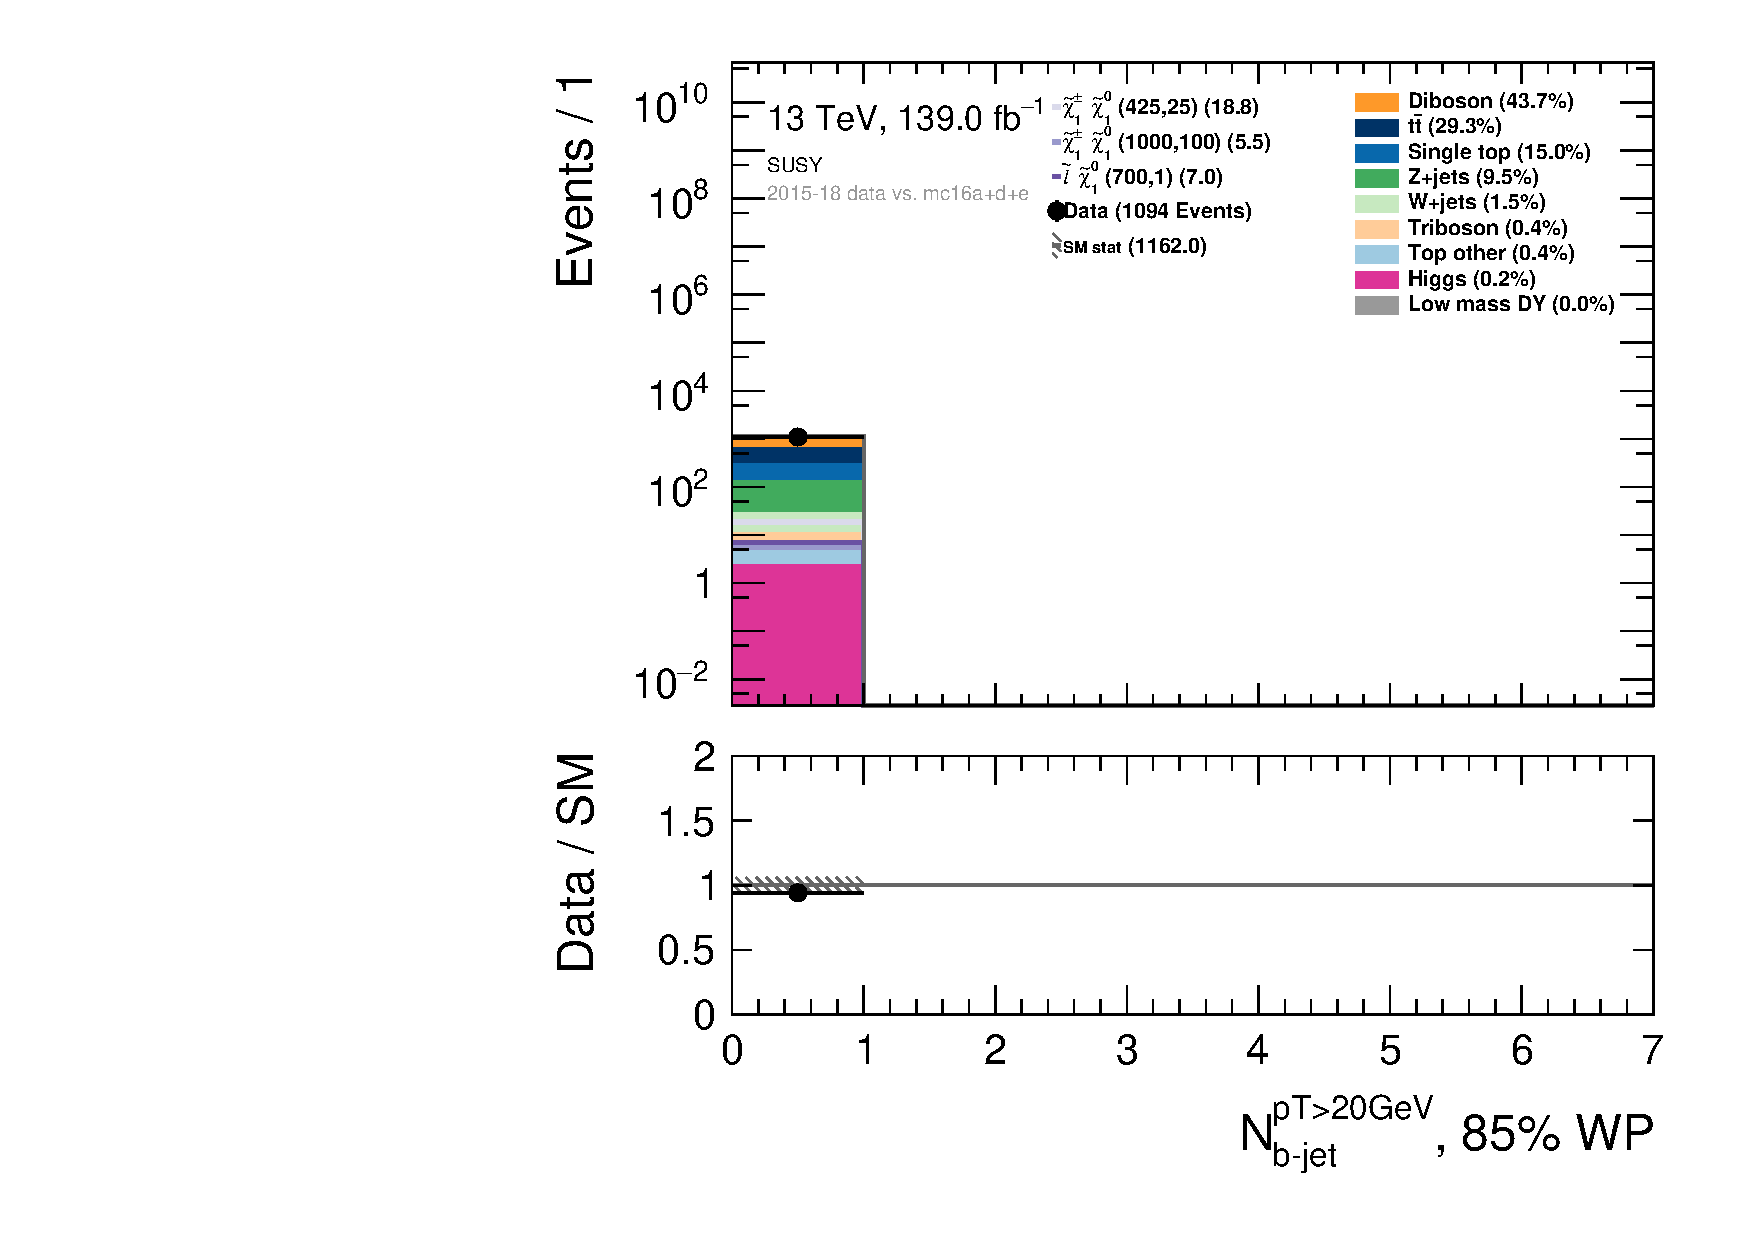
\includegraphics[width=\textwidth]{Figures/SUSYcuts/hist1d_nBJet20_MV2c10_FixedCutBEff_85_SUSY.pdf}
    \caption{Stransverse mass for chargino production via $W^\pm$.}
    \label{fig:my_label}
    \end{subfigure}
    \begin{subfigure}[t!]{0.49\textwidth}
        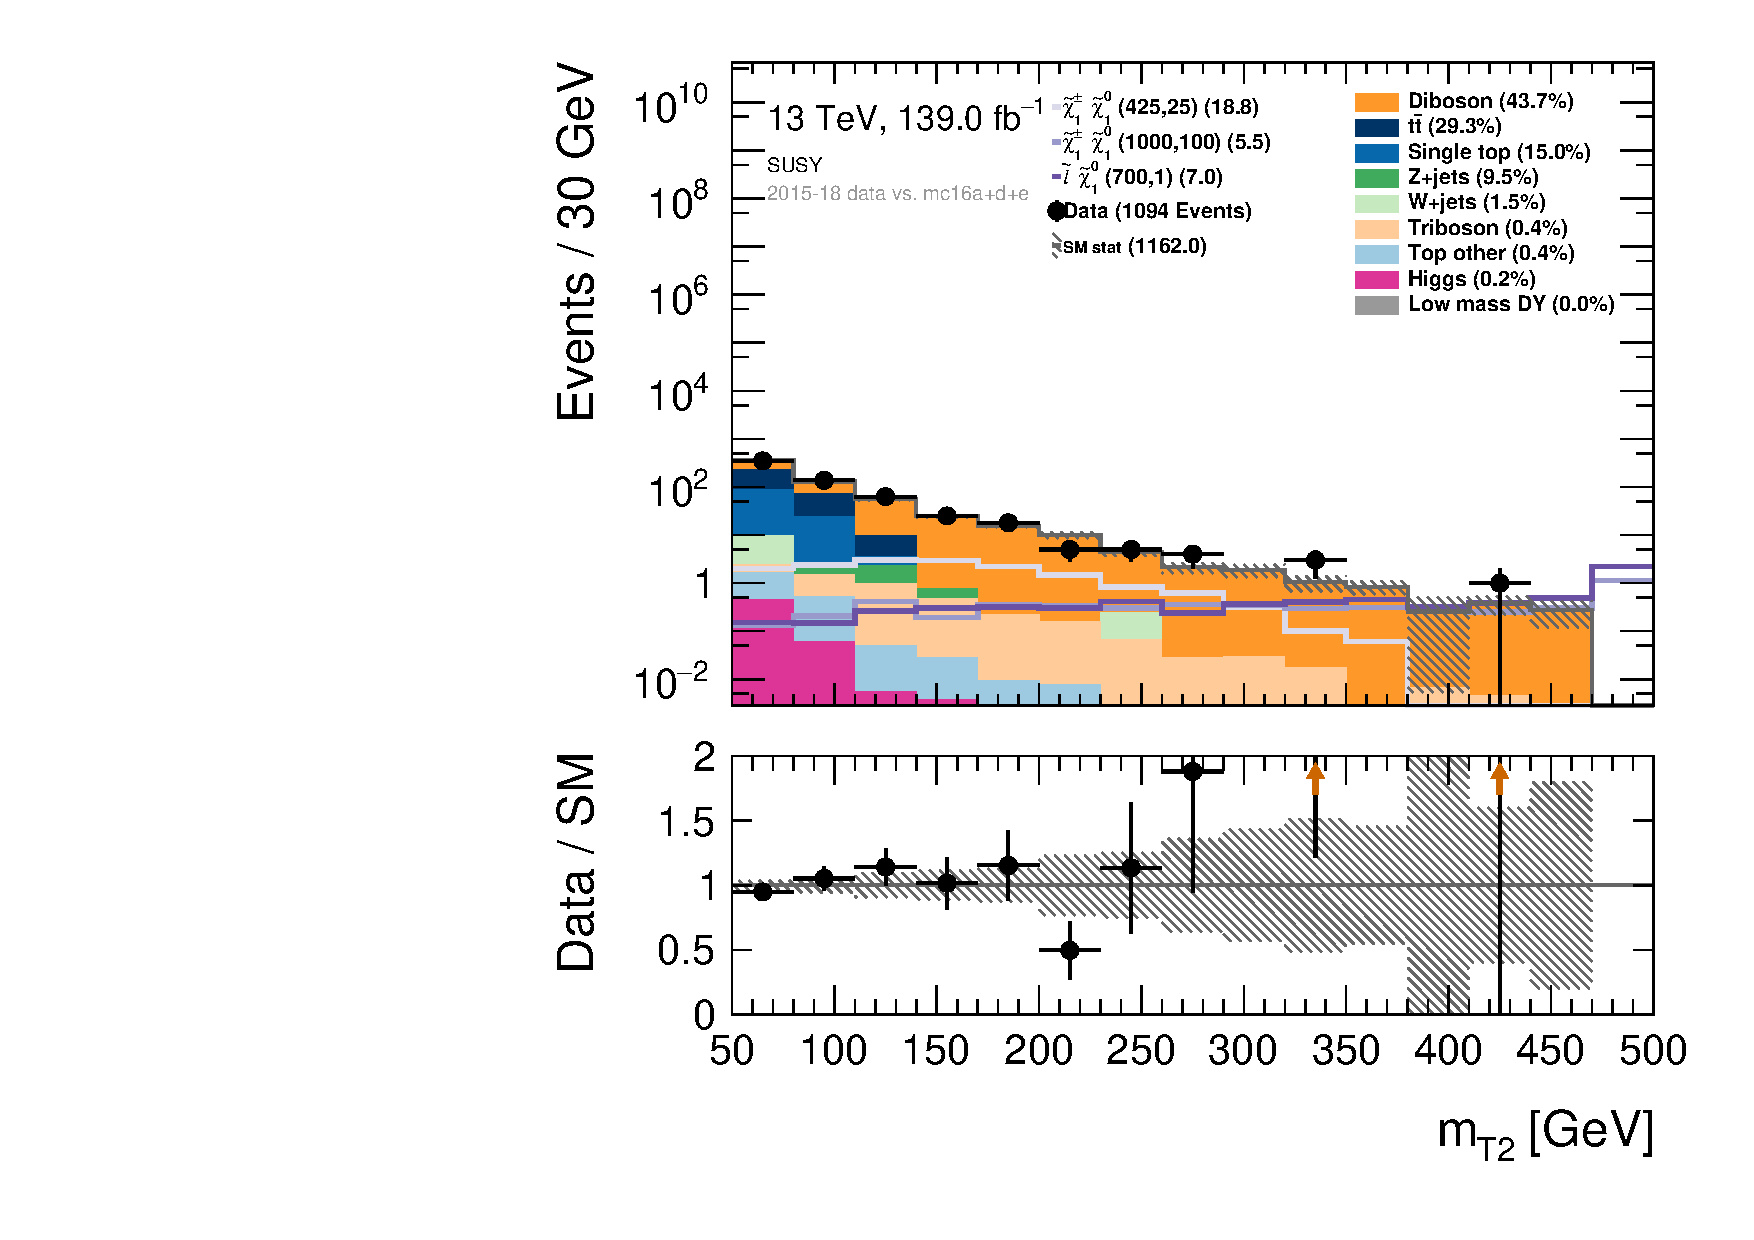
\includegraphics[width=\textwidth]{Figures/SUSYcuts/hist1d_mt2_SUSY.pdf}
    \caption{Missing transverse energy for mono-Z.}
    \label{fig:my_label}
    \end{subfigure}
    \caption{Plot of the four most important variables in direct slepton production with a cut on only two leptons with opposite charge in the final state.}
    \label{fig:cutandcountStepsSUSY}
\end{figure}
\restoregeometry
\end{comment}

















The same procedure was done for the mono-Z process, where we have applied the cuts from table \ref{tab:cutsDM} and we can see how much each cut affect the different contributions in table \ref{tab:cutflowDM}. 


\begin{table}[H]
    \centering
    \begin{tabular}{l l}\toprule
    \textbf{Variables} & \textbf{Cuts}\\
    \midrule
    \midrule
    Two leptons     &  OS with leading (subleading) $p_T >$ 30 (20) GeV\\
    $m_{ll}$     & 76 $< m_{ll} <$ 106 GeV\\
    $E_T^{miss}$ & $>$ 90 GeV\\
    $E_T^{miss}/H_T$ & $>$ 0.6\\
    $\Delta \phi (\Vec{p}_T^{ll}, E_T^{miss})$ & $>$ 2.7 radians\\
    $\Delta R_{ll}$ & $<$ 1.8\\
    Fractional $p_T$ difference & $|p_T^{ll} - p_T^{miss, jets}|/p_T^{ll} <$ 0.2\\
    b-jets & 0\\
    \bottomrule
     \end{tabular}
    \caption{Cuts added in the cut and count analysis taken from the publication for the mono-Z process \cite{monoZexclusion}.}
    \label{tab:cutsDM}
\end{table}

For the DM process, we have applied the cuts in table \ref{tab:cutsDM}, where we, as for the SUSY processes, demand to only have two leptons with opposite sign (but not necessarily the same flavor) in the final state together with missing transverse energy. In addition to the cut on number of leptons, we cut on the $p_T$ of the leptons, both the leading and subleading lepton. The cut on the subleading lepton will not affect anything because it is already done a cut at 25 GeV while handling the data for this thesis. This is shown in figure \ref{fig:mllDM} and table \ref{tab:cutflowDM}, where we can see that the distribution looks very similar as for the SUSY processes earlier in this chapter. We have demanded a Z-veto which we can see the results from in figure \ref{fig:metDM}. For both these cuts, we can see that Z+jets are the dominating background, where all the different backgrounds are reduced. 

\begin{figure}[H]
    \centering
    \begin{subfigure}[t!]{0.49\textwidth}
        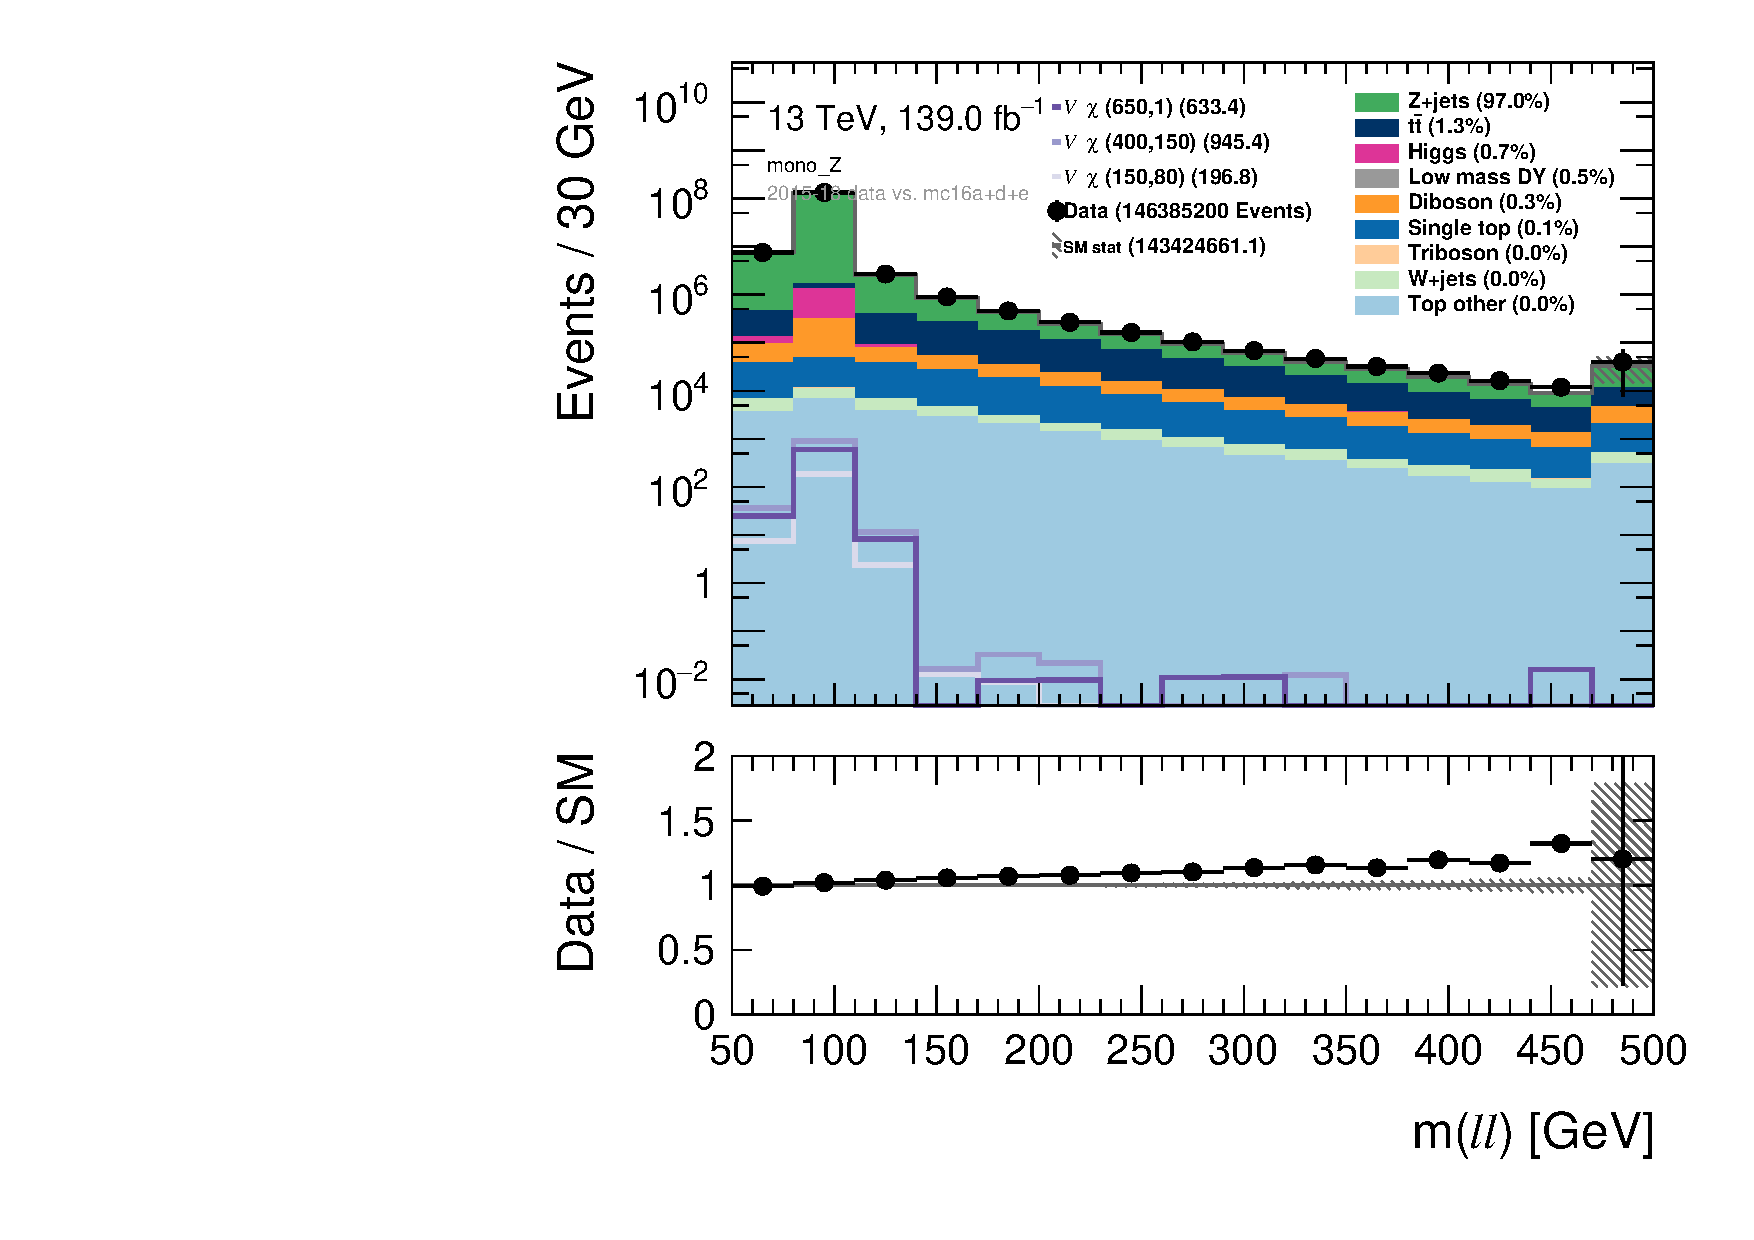
\includegraphics[width=\textwidth]{Figures/MonoZcuts/hist1d_mll_mono_Z.pdf}
    \caption{Invariant mass.}
    \label{fig:mllDM}
    \end{subfigure}
    \begin{subfigure}[t!]{0.49\textwidth}
        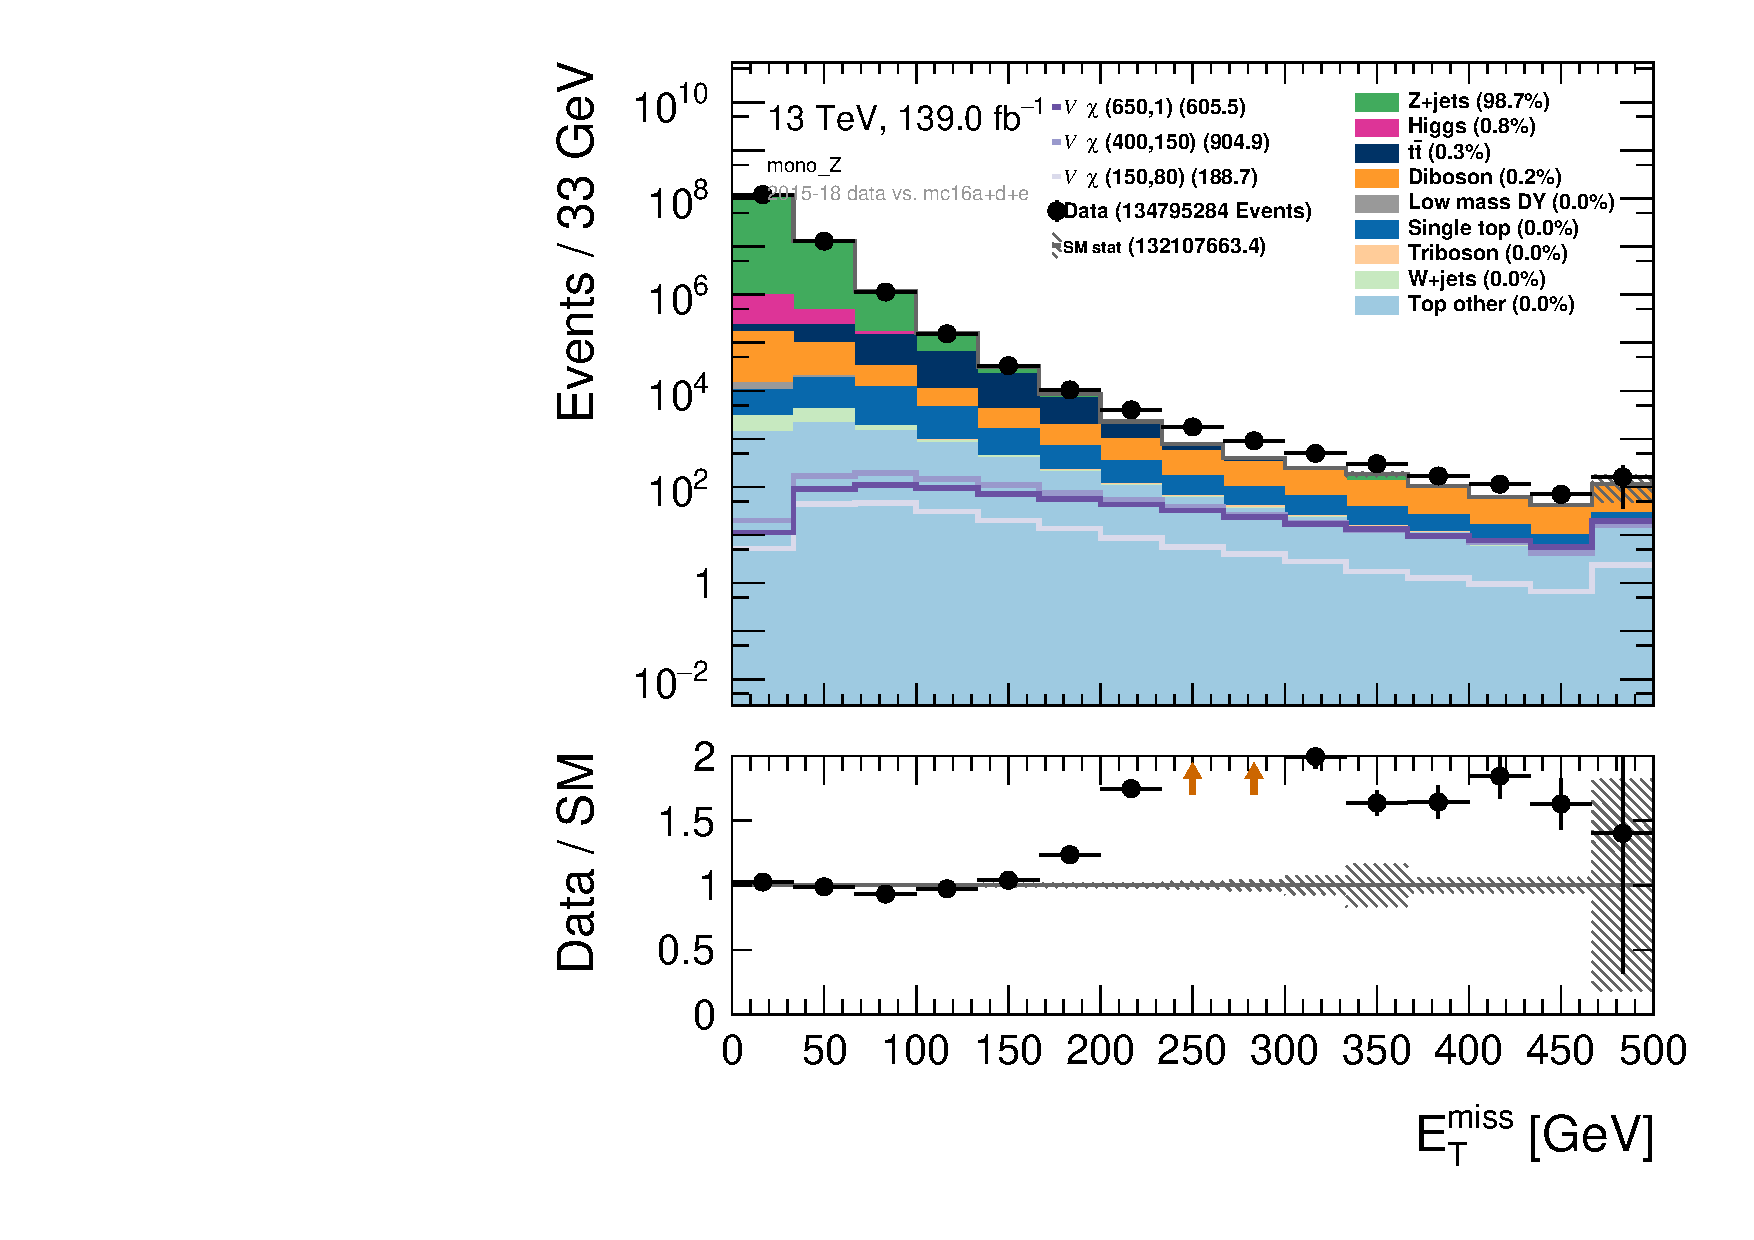
\includegraphics[width=\textwidth]{Figures/MonoZcuts/hist1d_met_Et_mono_Z_1.pdf}
    \caption{Missing transverse energy.}
    \label{fig:metDM}
    \end{subfigure}
    \caption{Plot of different distributions after applying the cuts on 2L, OS, $p_T$ of the two leptons and invariant mass.}
    \label{fig:stepsDM1}
\end{figure}

We also do a slightly more gentle cut on the missing transverse energy for this process than the SUSY processes because we have several other MET dependent variables for mono-Z. One of these are $E_T^{miss}/H_T$. After applying the MET cut, we can see that the Z+jets are less dominating, but since the MET/$H_T$ reduces the $t\Bar{t}$ background, the Z+jets becomes more dominating again. The results are shown in figure \ref{fig:stepsDM2}.

\begin{figure}[H]
    \centering
    \begin{subfigure}[t!]{0.49\textwidth}
        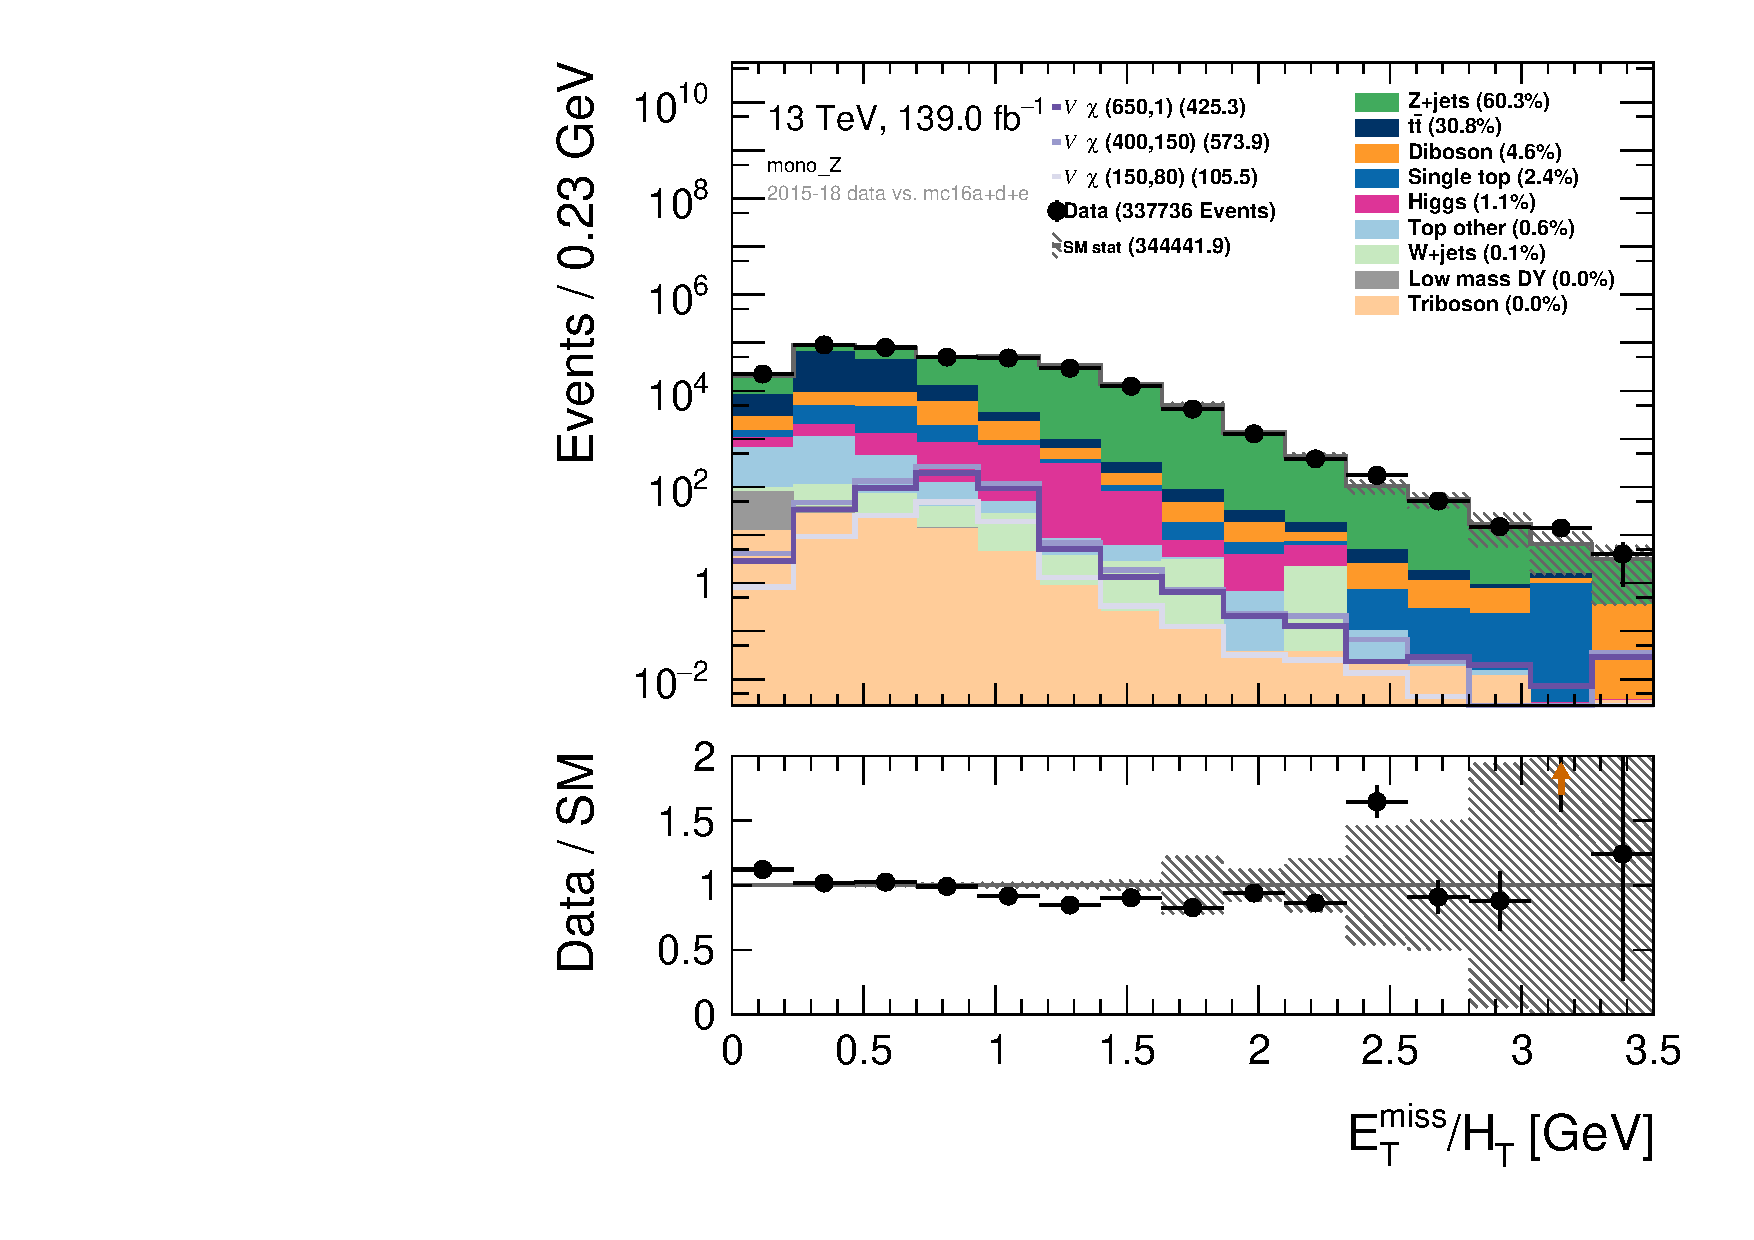
\includegraphics[width=\textwidth]{Figures/MonoZcuts/hist1d_met_HT_mono_Z.pdf}
    \caption{The ratio between $E_T^{miss}$ and $H_T$.}
    \label{fig:metHTDM}
    \end{subfigure}
    \begin{subfigure}[t!]{0.49\textwidth}
        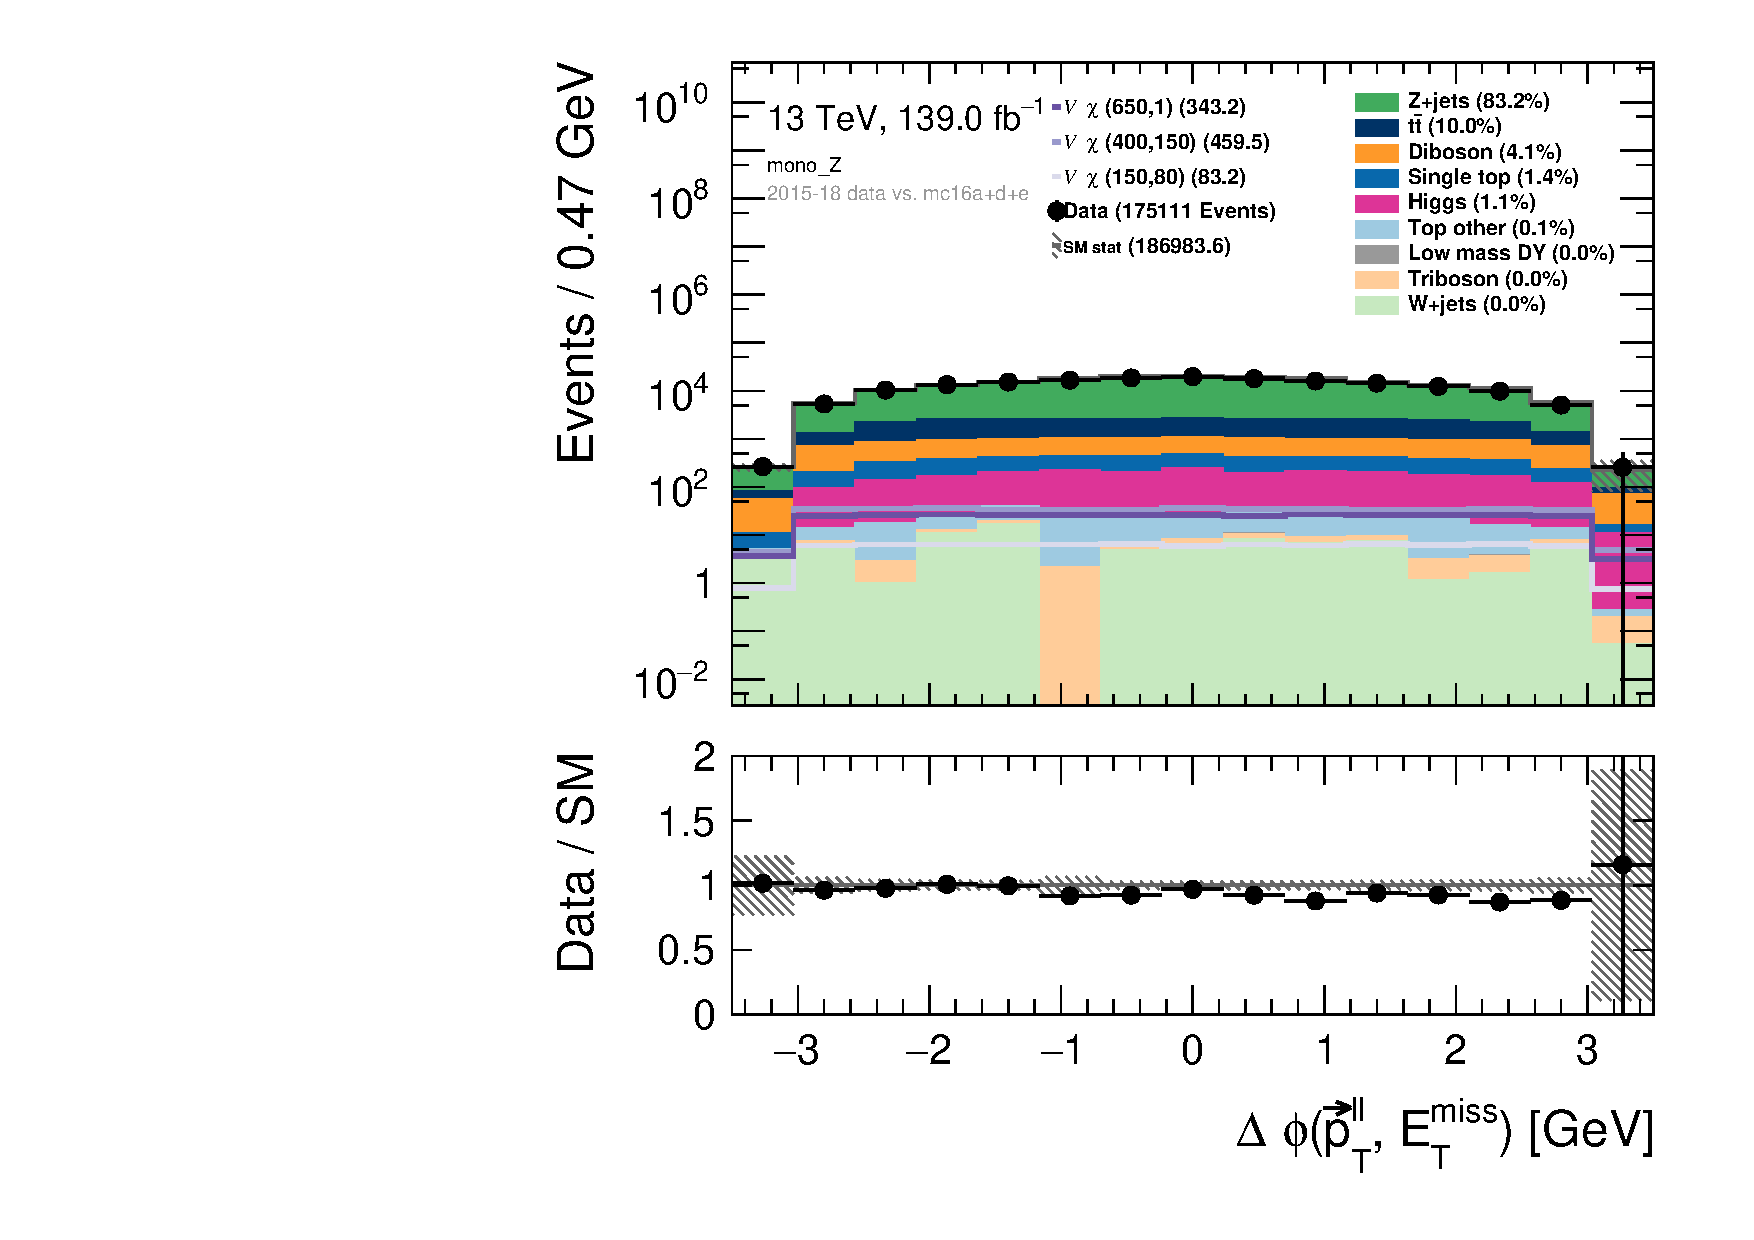
\includegraphics[width=\textwidth]{Figures/MonoZcuts/hist1d_deltaPhi_mono_Z.pdf}
    \caption{The azimuthal angle difference between the dilepton system and $E_T^{miss}$.}
    \label{fig:delphiDM}
    \end{subfigure}
    \caption{Plot of different distributions after applying the cuts on MET and MET/$H_T$.}
    \label{fig:stepsDM2}
\end{figure}


The next cut that is applied is $\Delta \phi (\Vec{p}_T^{ll}, E_T^{miss})$, where the two leptons also have to be close to each other, which can be demand by $\Delta R_{ll}$. $\Delta \phi$ is also one of the MET dependent variables we have used for the mono-Z process. The results after applying these cuts are presented in figure \ref{fig:stepsDM3} and as we can see, the Z+jets keeps being the dominating background. 




\begin{figure}[H]
    \centering
    \begin{subfigure}[t!]{0.49\textwidth}
        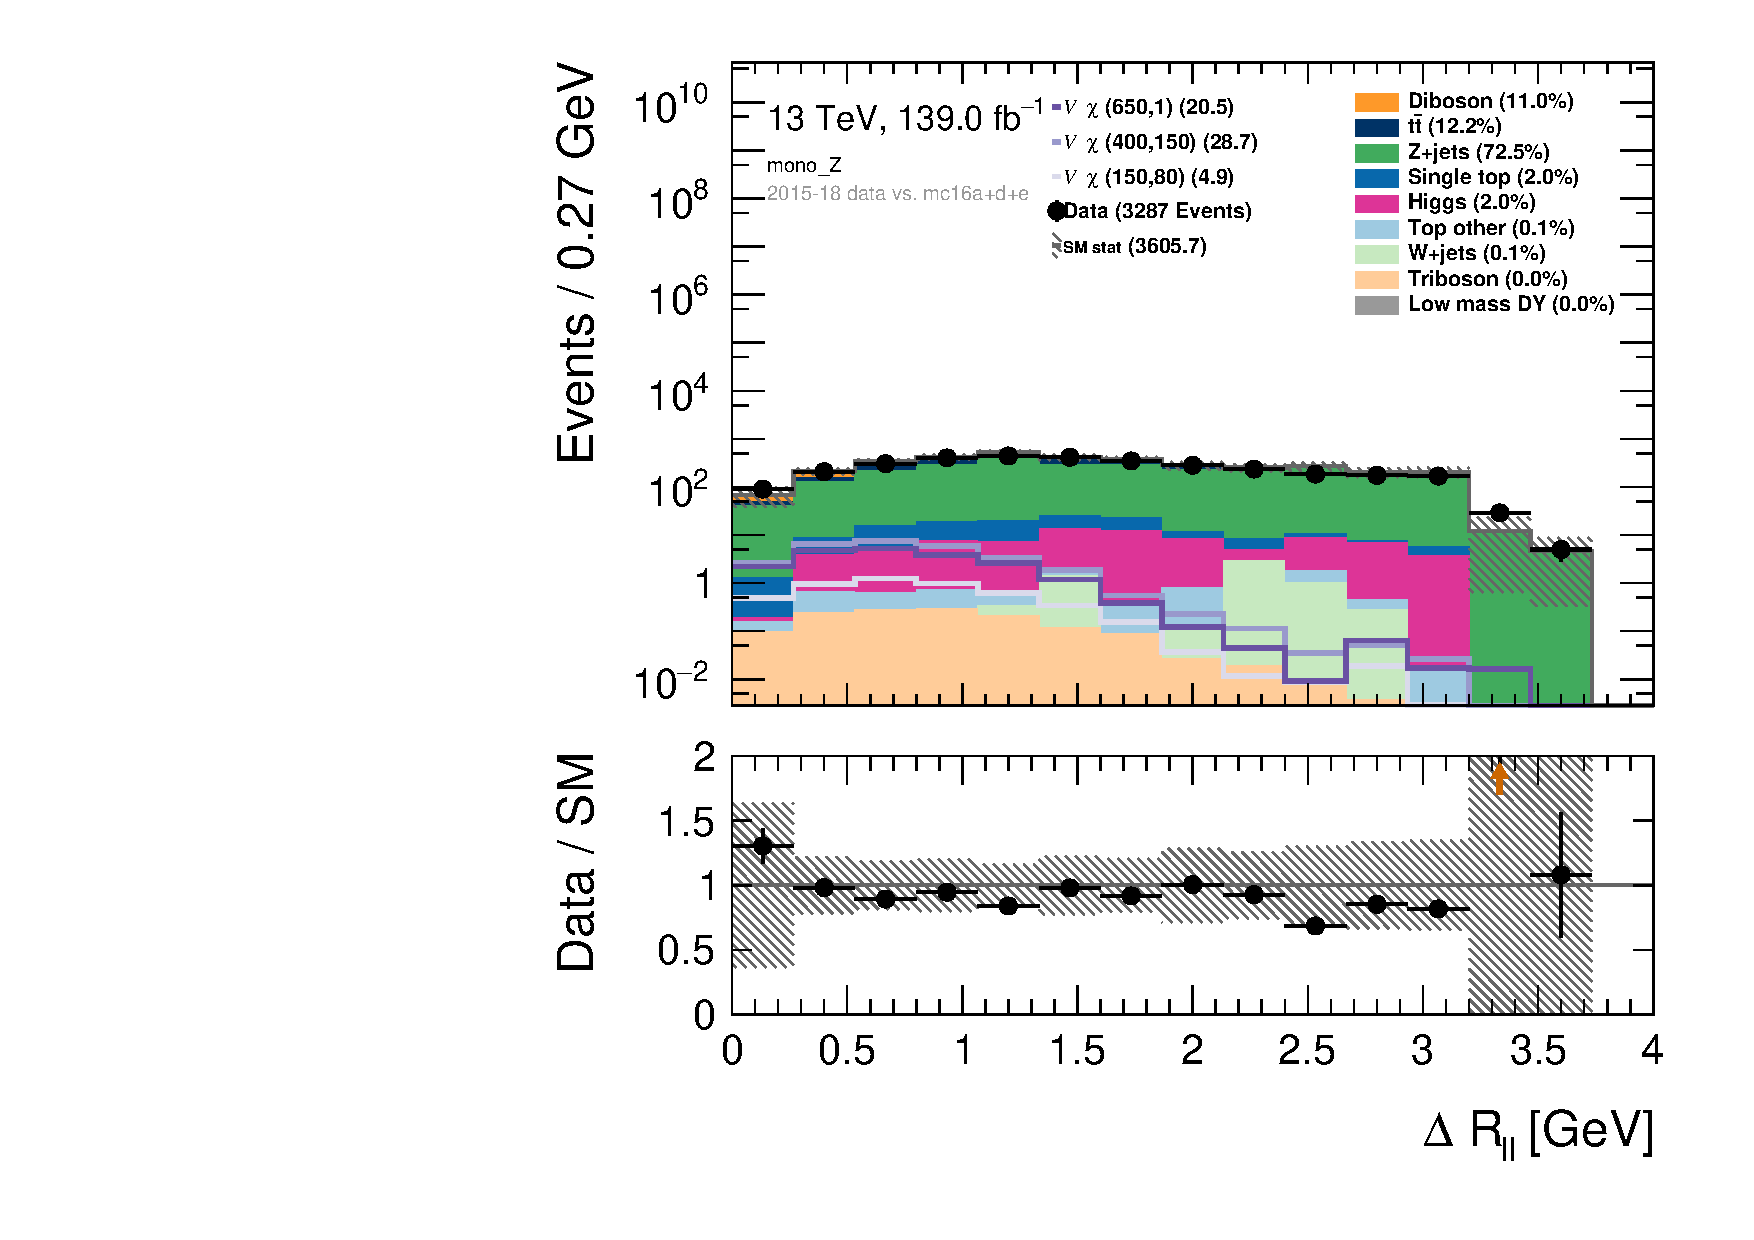
\includegraphics[width=\textwidth]{Figures/MonoZcuts/hist1d_deltaRll_mono_Z.pdf}
    \caption{Distance between the two leptons.}
    \label{fig:delRllDM}
    \end{subfigure}
    \begin{subfigure}[t!]{0.49\textwidth}
        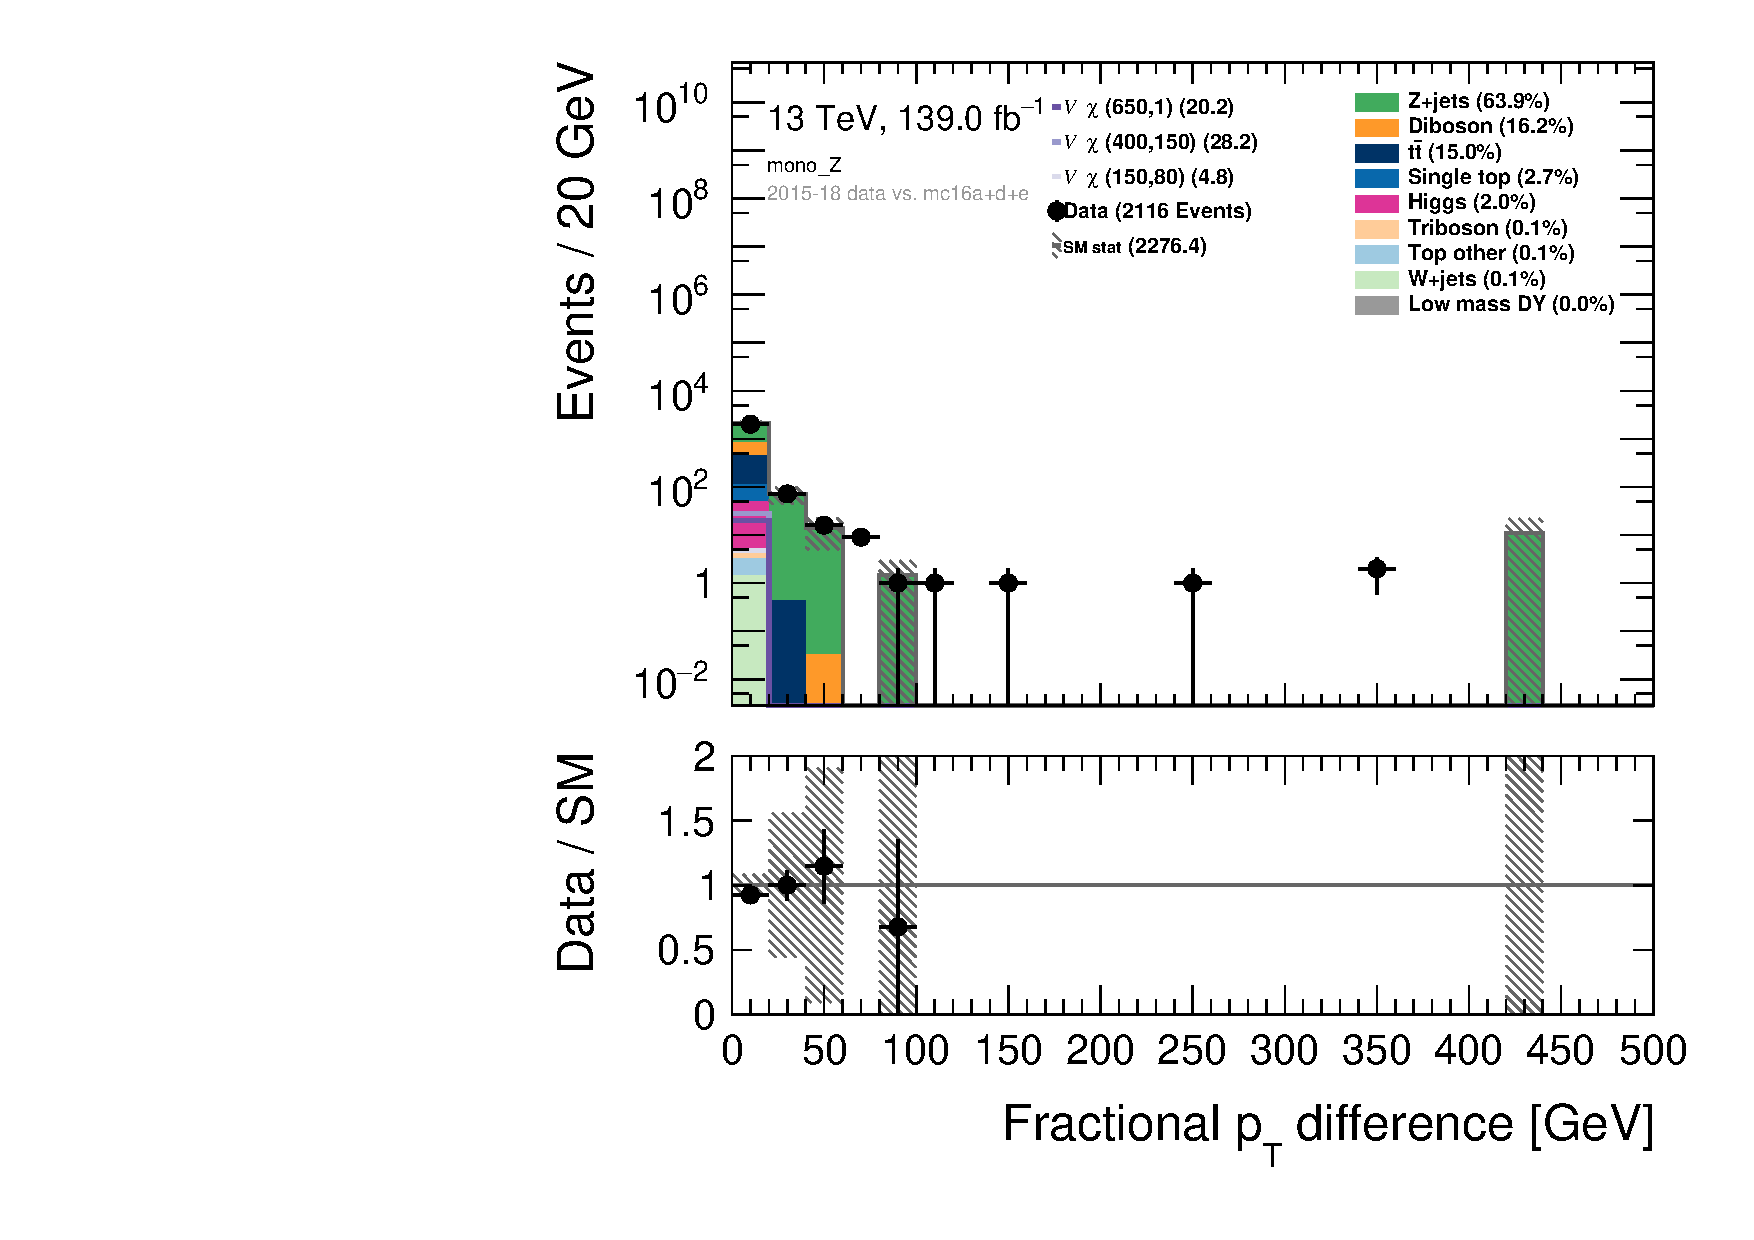
\includegraphics[width=\textwidth]{Figures/MonoZcuts/hist1d_pTdiff_mono_Z.pdf}
    \caption{The difference between the dilepton $p_T$, the selected jets $p_T$ and the vector sum of $\Vec{E}_T^{miss}$.}
    \label{fig:pTdiffDM}
    \end{subfigure}
    \caption{Plot of different distributions after applying the cuts on $\Delta \phi$ and $\Delta R_{ll}$}
    \label{fig:stepsDM3}
\end{figure}


The last cuts we apply is a cut on the fractional $p_T$ difference and a b-jet veto. The results from adding the $p_T$ cut are presented in figure \ref{fig:stepsDM4}, while the final results including b-jet veto is presented in figure \ref{fig:cutandcountMONA} later in this section. We can also see for both these cases that the dominating background have become diboson, which is the same as for the SUSY processes. 

\begin{figure}[H]
    \centering
        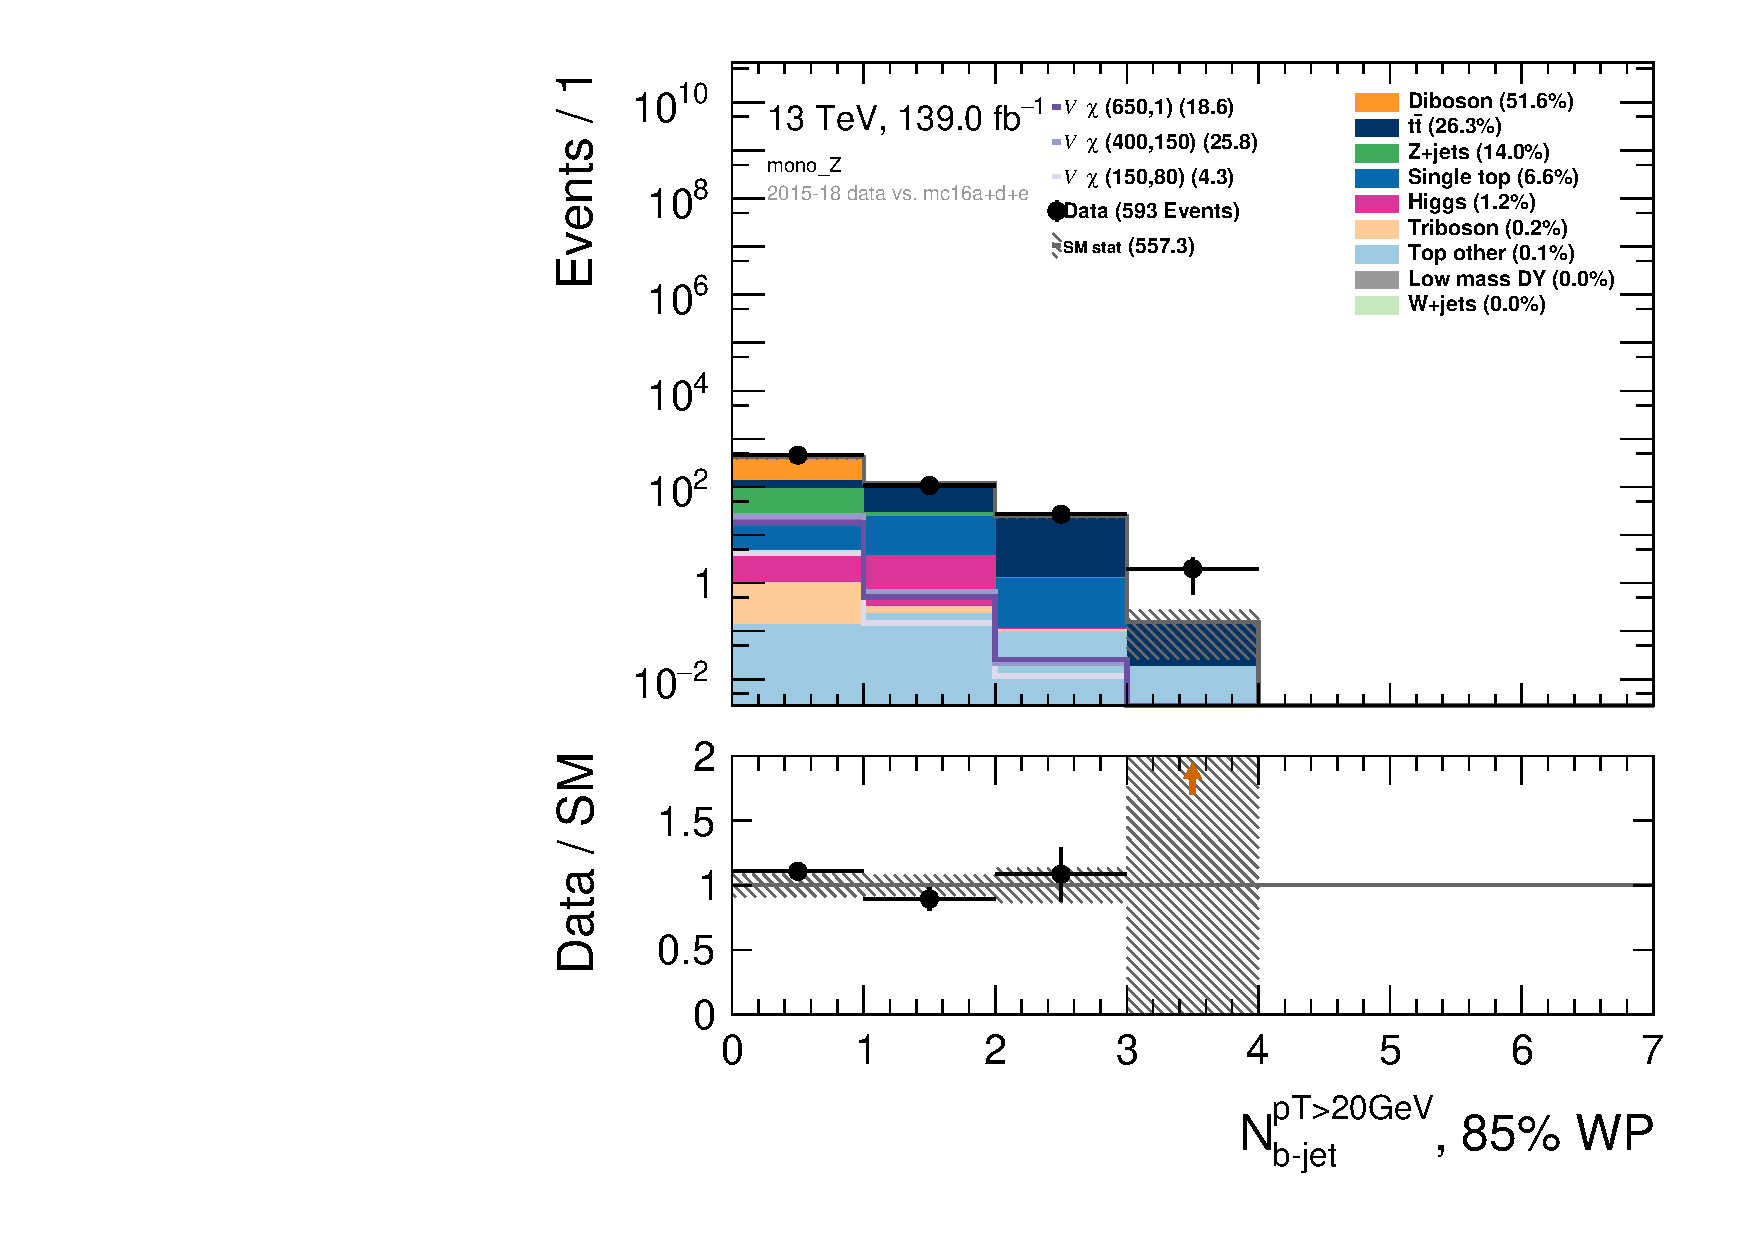
\includegraphics[width=0.5\textwidth]{Figures/MonoZcuts/hist1d_nBJet20_MV2c10_FixedCutBEff_85_mono_Z.pdf}
    \caption{Plot of the distribution of number of b-tagged jets after applying the cuts on fractional $p_T$ difference.}
    \label{fig:stepsDM4}
\end{figure}

For the signals in this case, which is maybe easier to see in table \ref{tab:cutflowDM}, we can see that it is reduced a lot. This is of course not what we want to obtain, but it is also expected after doing that many cuts as we have done.

\begin{landscape}
\begin{table}[H]
    \centering
    %\rotatebox{90}{
    \begin{tabular}{l l l l l l l l l}
    \toprule
    \textbf{Sample} & \textbf{2L + OS + $\mathbf{p_T}$} & $\mathbf{m_{ll}}$ & \textbf{MET} & \textbf{met/$\mathbf{H_T}$} & $\mathbf{\Delta \phi}$ & $\mathbf{\Delta R_{ll}}$ & \textbf{$\mathbf{p_T}$} \textbf{diff} & \textbf{b-jets} \\
    \midrule
    \midrule
        DY &  674647.170 & 7035.028 & 79.252 & 0.448 & 0.000 & 0.000 & 0.000 & 0.000\\
        Higgs & 1052061.840 & 1014012.858 & 3834.027 & 2116.006 & 73.416 & 46.198 & 6.942 & 3.467\\
        Single top & 189826.764 & 38267.988 & 8246.807 & 2620.670 & 73.820 & 60.859 & 36.895 & 14.845\\
        ttbar & 1854383.568 & 398898.217 & 106187.071 & 18667.204 & 439.750 & 342.455 & 146.530 & 42.570\\
        Zjets & 139141315.583 & 130368076.145 & 207856.769 & 155565.299 & 2613.607 & 1454.461 & 77.839 & 72.669\\
        Top other & 26411.801 & 6865.785 & 2104.230 & 211.226 & 3.570 & 1.880 & 0.492 & 0.136\\
        Wjets & 17813.414 & 4191.918 & 198.881 & 72.288 & 5.306 & 1.421 & 0.000 & 0.000\\
        Triboson & 528.623 & 211.477 & 81.766 & 27.851 & 1.406 & 1.332 & 0.999 & 0.900\\
        Diboson & 467672.290 & 270103.987 & 15853.093 & 7702.570 & 394.866 & 367.781 & 287.632 & 278.123\\
        Data & 146385200.000 & 134795284.000 & 337736.000 & 175111.000 & 3287.000 & 2116.000 & 593.000 & 457.000\\
        $( V, \chi) (150, 80)$ & 196.844 & 188.682 & 105.505 & 83.150 & 4.866 & 4.765 & 4.325 & 4.166\\
        $( V, \chi) (400, 150)$ & 945.406 & 904.916 & 573.904 & 459.476 & 28.740 & 28.194 & 25.789 & 25.124\\
        $( V, \chi) (650, 1)$  & 633.417 & 605.474 & 425.291 & 343.235 & 20.533 & 20.193 & 18.566 & 18.019\\
        \bottomrule
    \end{tabular}
    %}
    \caption{A cut flow overview after applying the different cuts in table \ref{tab:cutsDM}.}
    \label{tab:cutflowDM}
\end{table}
\end{landscape}





\begin{comment}


\newgeometry{twoside,inner=3cm,outer=2cm}
\begin{figure}[H]
%\begin{minipage}{2\textwidth}
%\begin{adjustwidth}{-3cm}{-3cm}
\centering
%\advance\leftskip-4cm 
%\advance\rightskip-4cm 
    \begin{subfigure}[t!]{0.49\textwidth}
        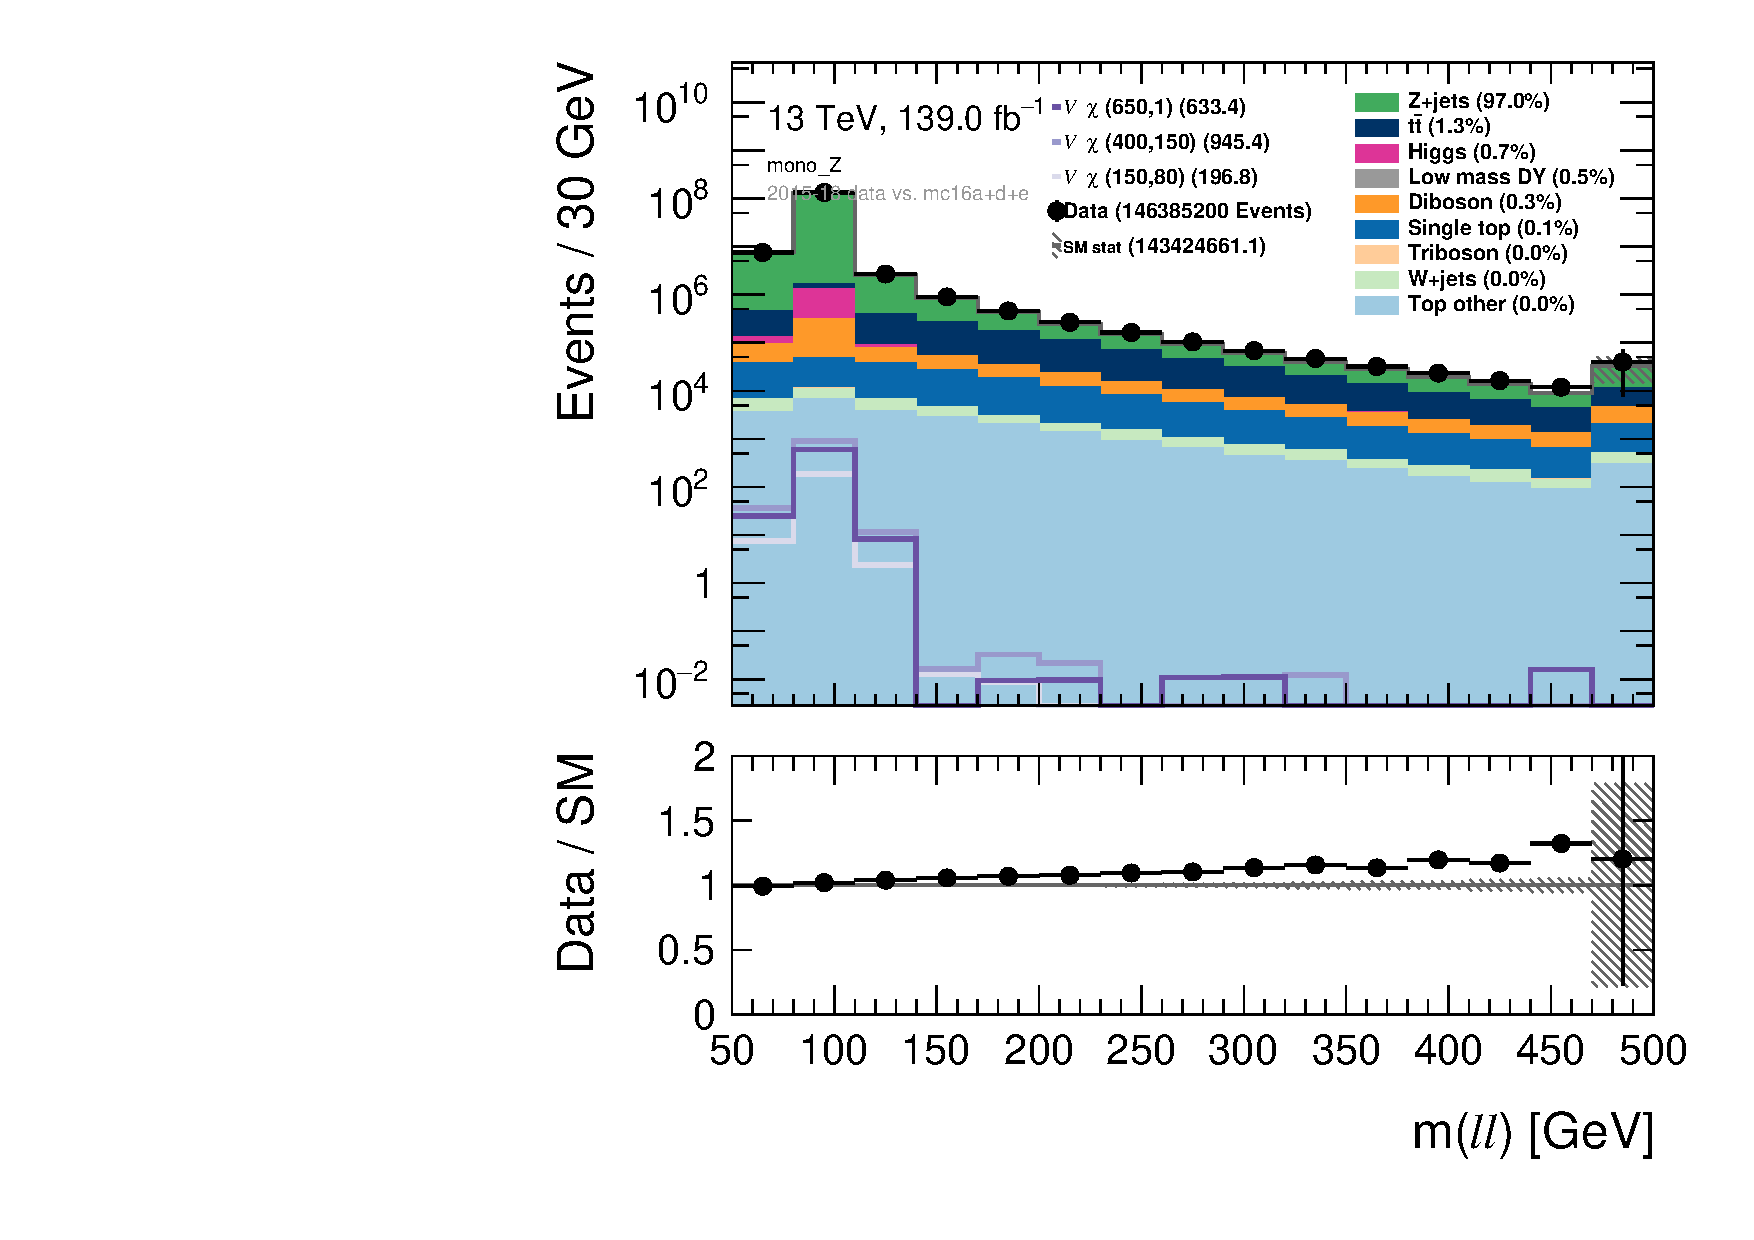
\includegraphics[width=\textwidth]{Figures/MonoZcuts/hist1d_mll_mono_Z.pdf}
    \caption{Stransverse mass for direct slepton production.}
    \label{fig:my_label}
    \end{subfigure}
    \begin{subfigure}[t!]{0.49\textwidth}
        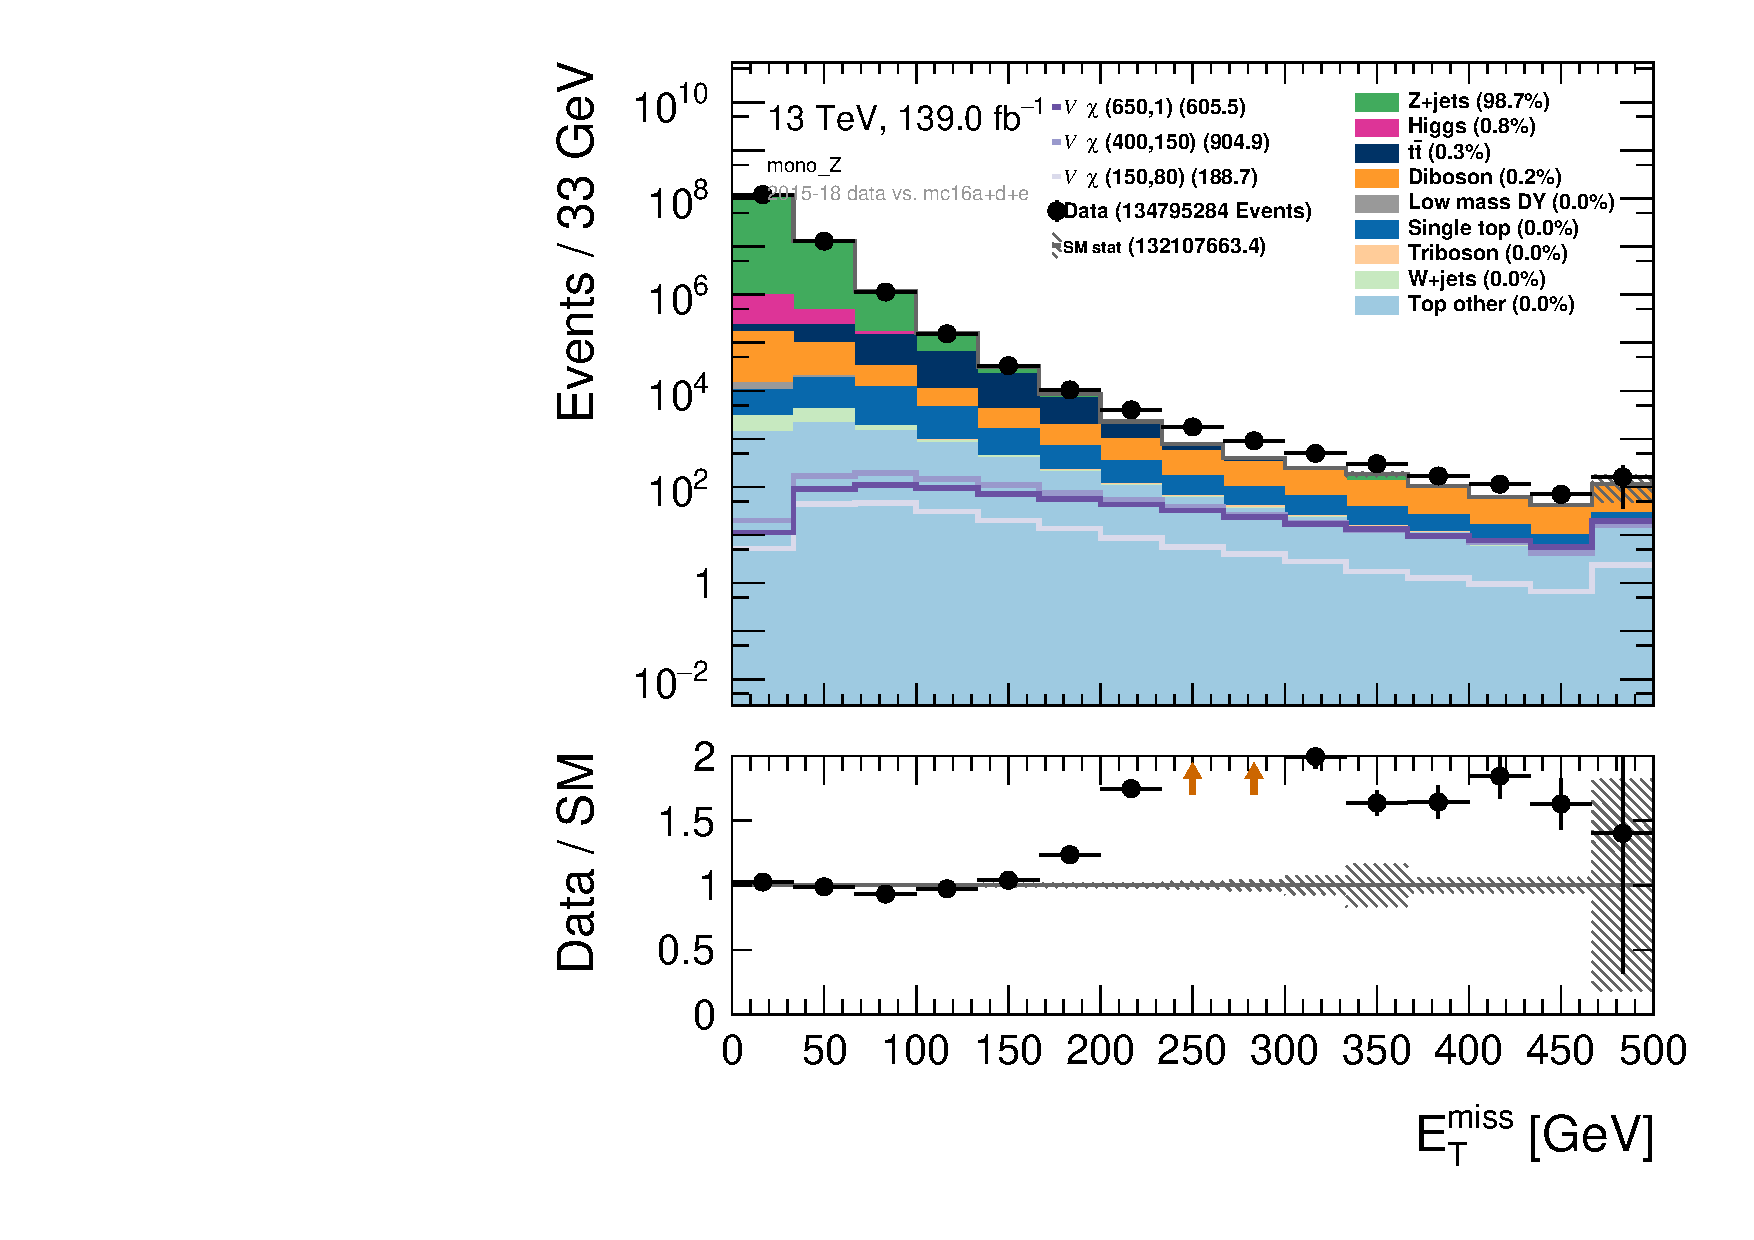
\includegraphics[width=\textwidth]{Figures/MonoZcuts/hist1d_met_Et_mono_Z_1.pdf}
    \caption{Stransverse mass for chargino production via $\Tilde{l}/\Tilde{\nu}$.}
    \label{fig:my_label}
    \end{subfigure}
    \\
    \begin{subfigure}[t!]{0.49\textwidth}
        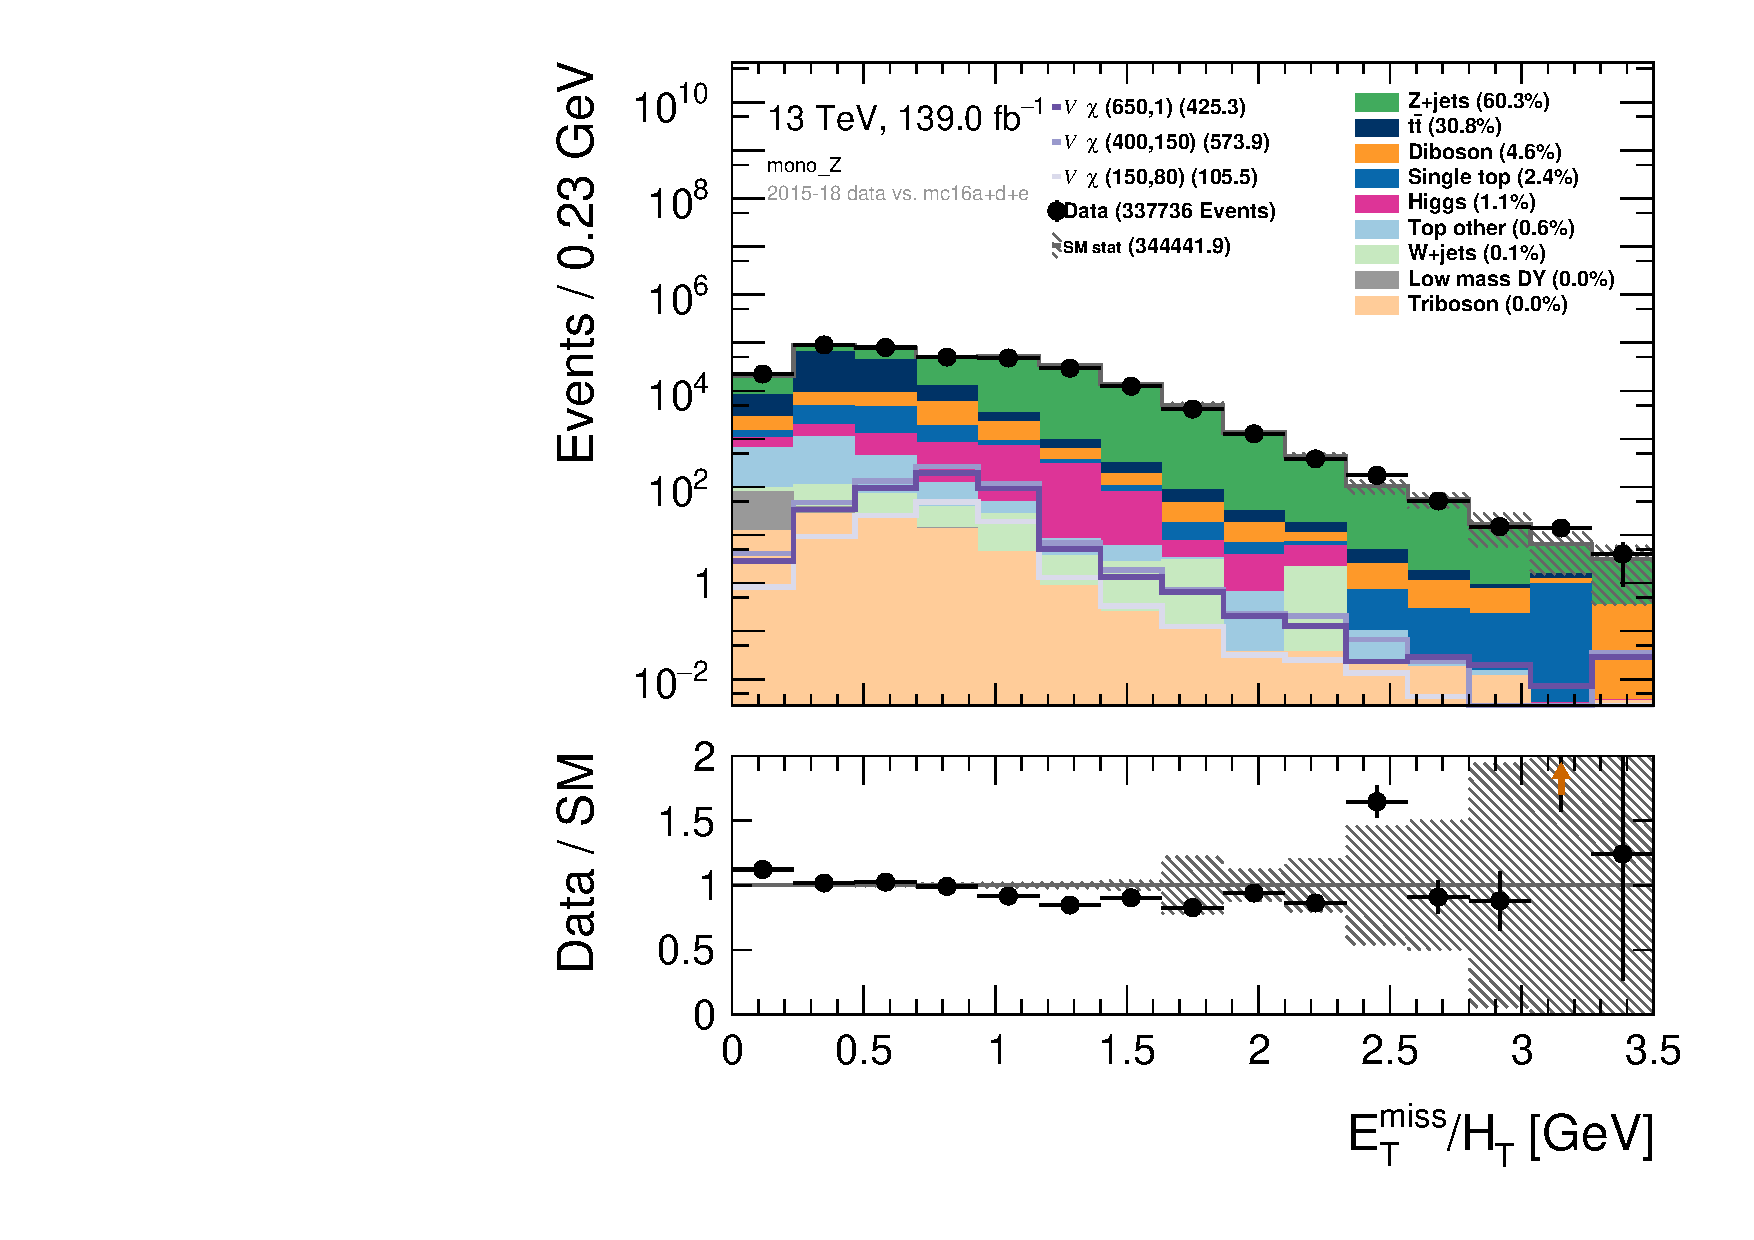
\includegraphics[width=\textwidth]{Figures/MonoZcuts/hist1d_met_HT_mono_Z.pdf}
    \caption{Stransverse mass for chargino production via $W^\pm$.}
    \label{fig:my_label}
    \end{subfigure}
    \begin{subfigure}[t!]{0.49\textwidth}
        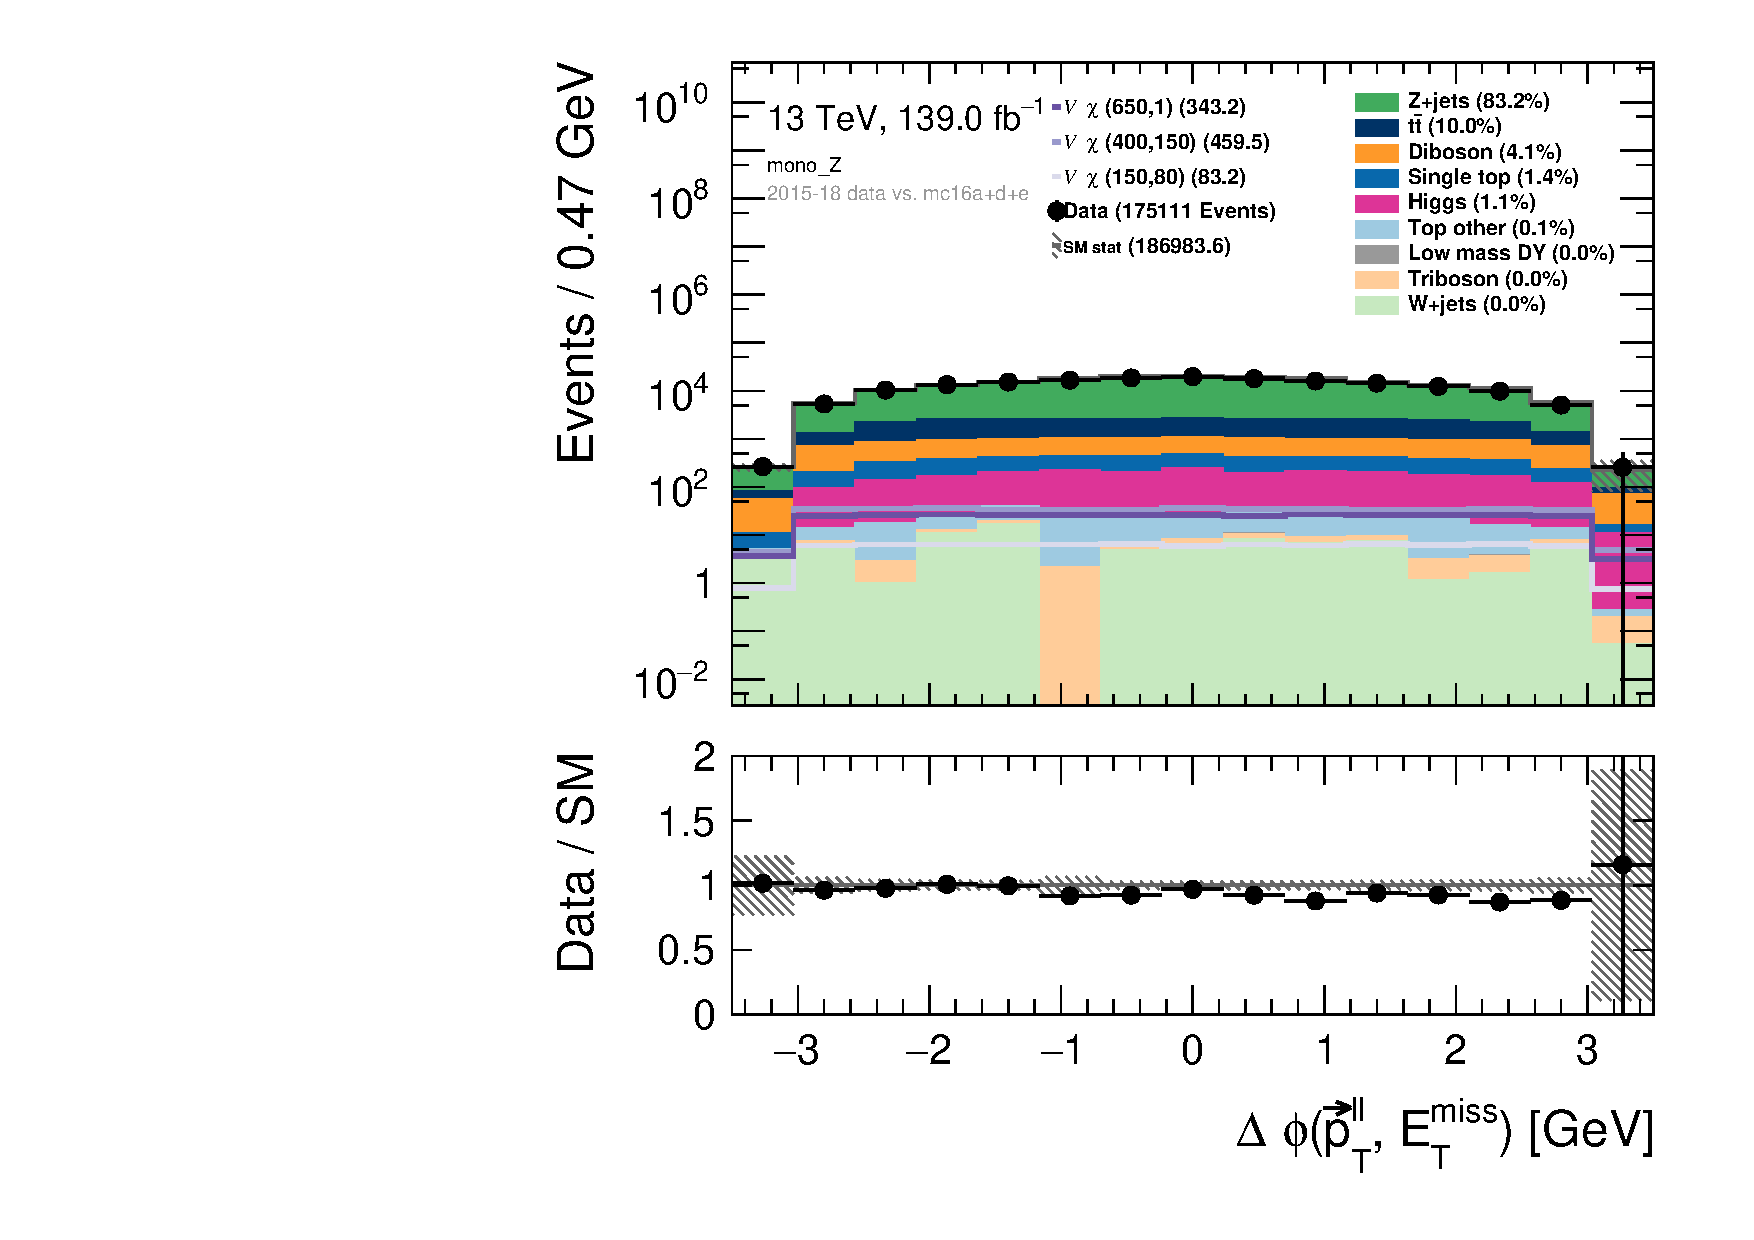
\includegraphics[width=\textwidth]{Figures/MonoZcuts/hist1d_deltaPhi_mono_Z.pdf}
    \caption{Missing transverse energy for mono-Z.}
    \label{fig:my_label}
    \end{subfigure}
    \\
    \begin{subfigure}[t!]{0.49\textwidth}
        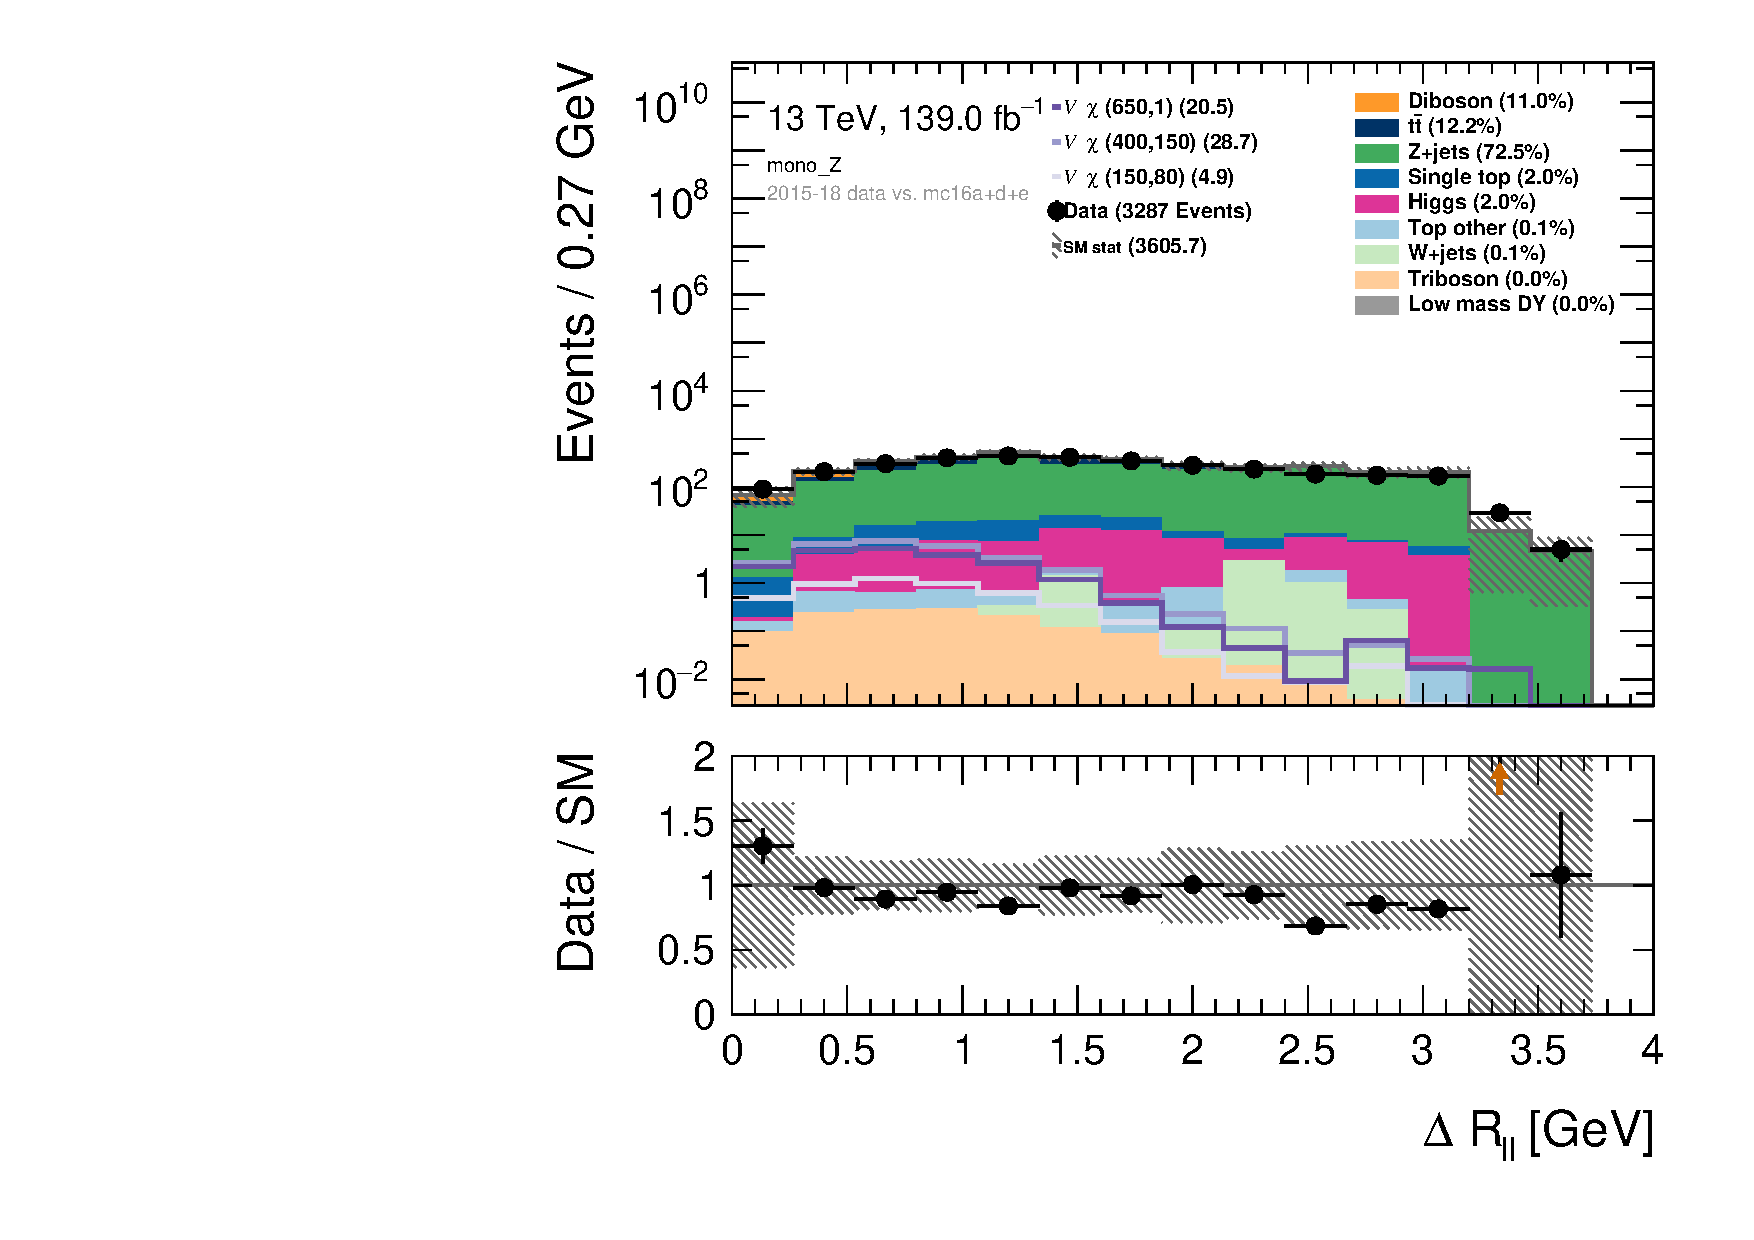
\includegraphics[width=\textwidth]{Figures/MonoZcuts/hist1d_deltaRll_mono_Z.pdf}
    \caption{Stransverse mass for chargino production via $W^\pm$.}
    \label{fig:my_label}
    \end{subfigure}
    \begin{subfigure}[t!]{0.49\textwidth}
        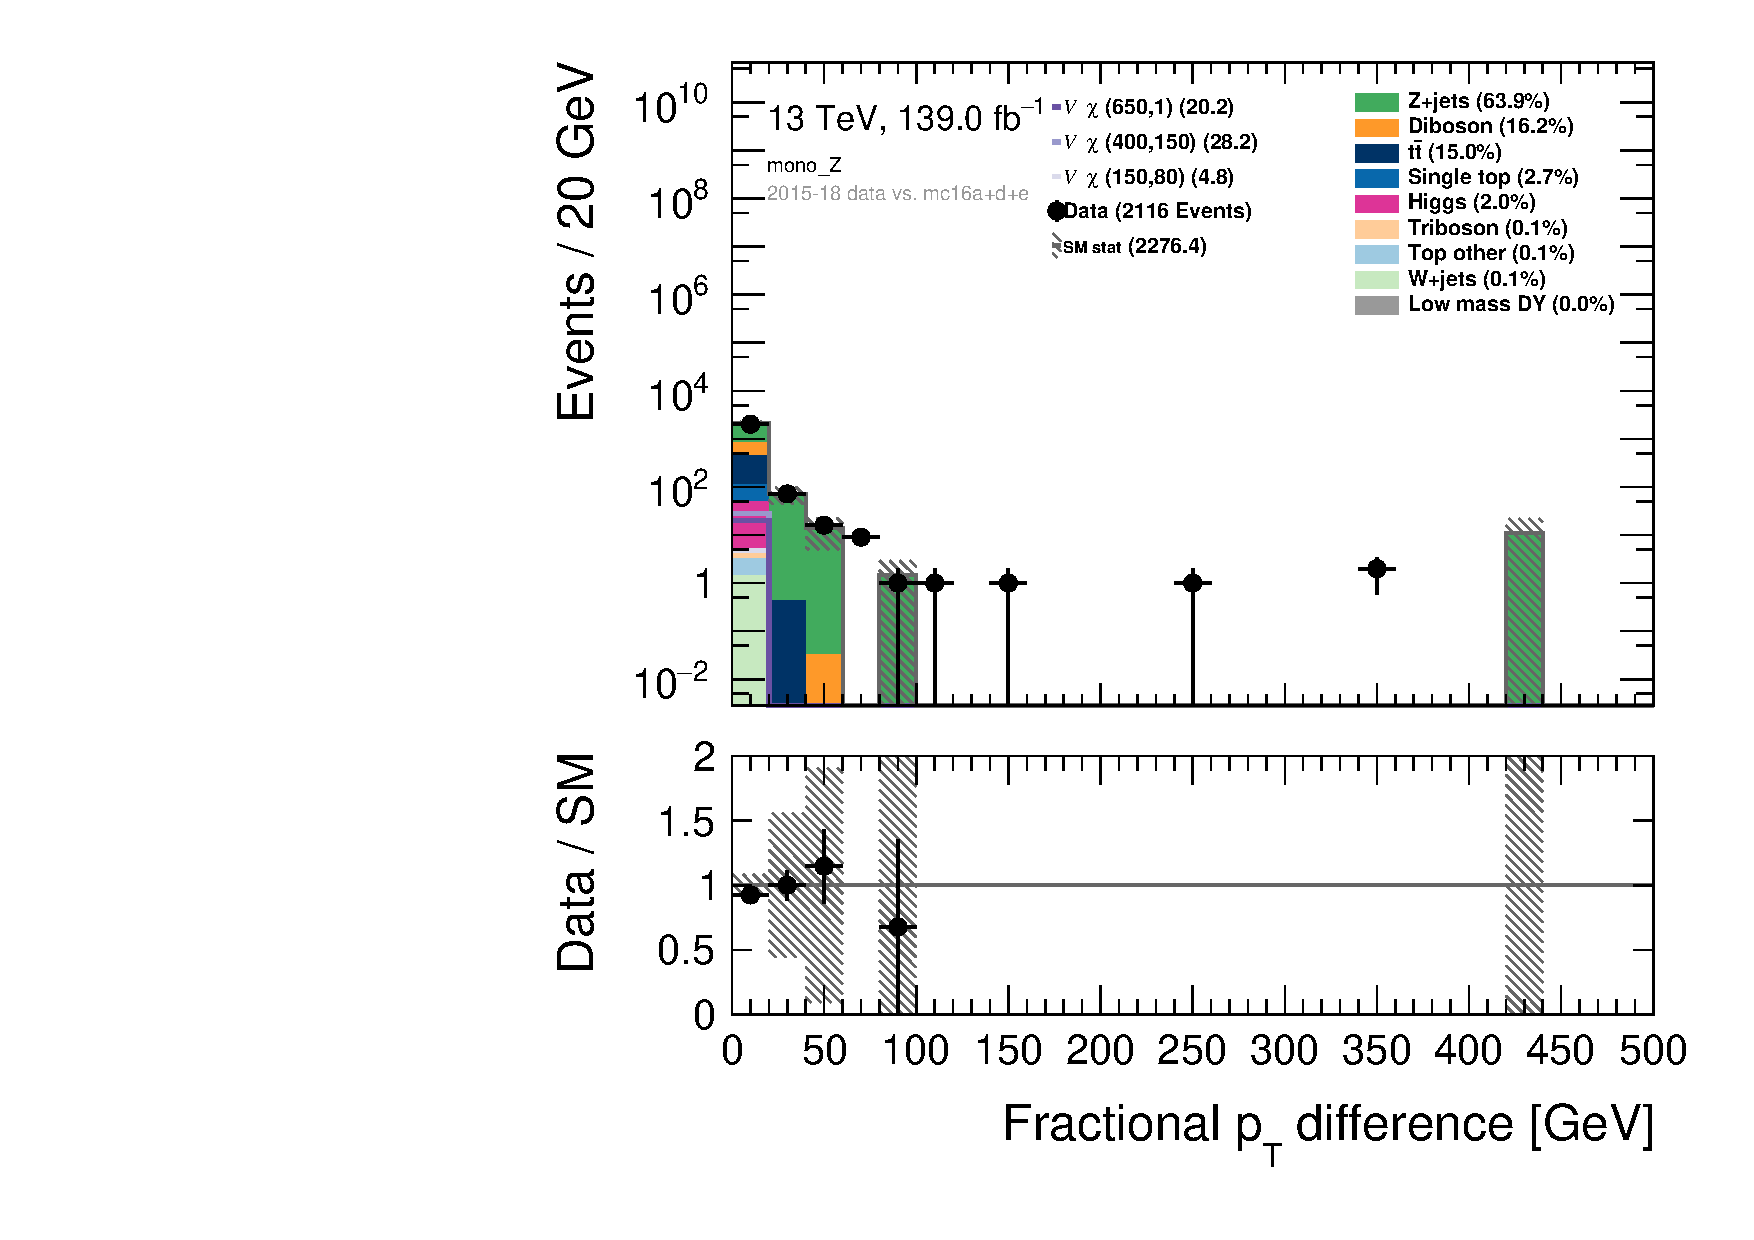
\includegraphics[width=\textwidth]{Figures/MonoZcuts/hist1d_pTdiff_mono_Z.pdf}
    \caption{Missing transverse energy for mono-Z.}
    \label{fig:my_label}
    \end{subfigure}
\end{figure}
\restoregeometry


\newgeometry{twoside,inner=3cm,outer=2cm}
\begin{figure}[H] \ContinuedFloat
%\begin{minipage}{2\textwidth}
%\begin{adjustwidth}{-3cm}{-3cm}
\centering
%\advance\leftskip-4cm 
%\advance\rightskip-4cm 
    \begin{subfigure}[t!]{0.49\textwidth}
        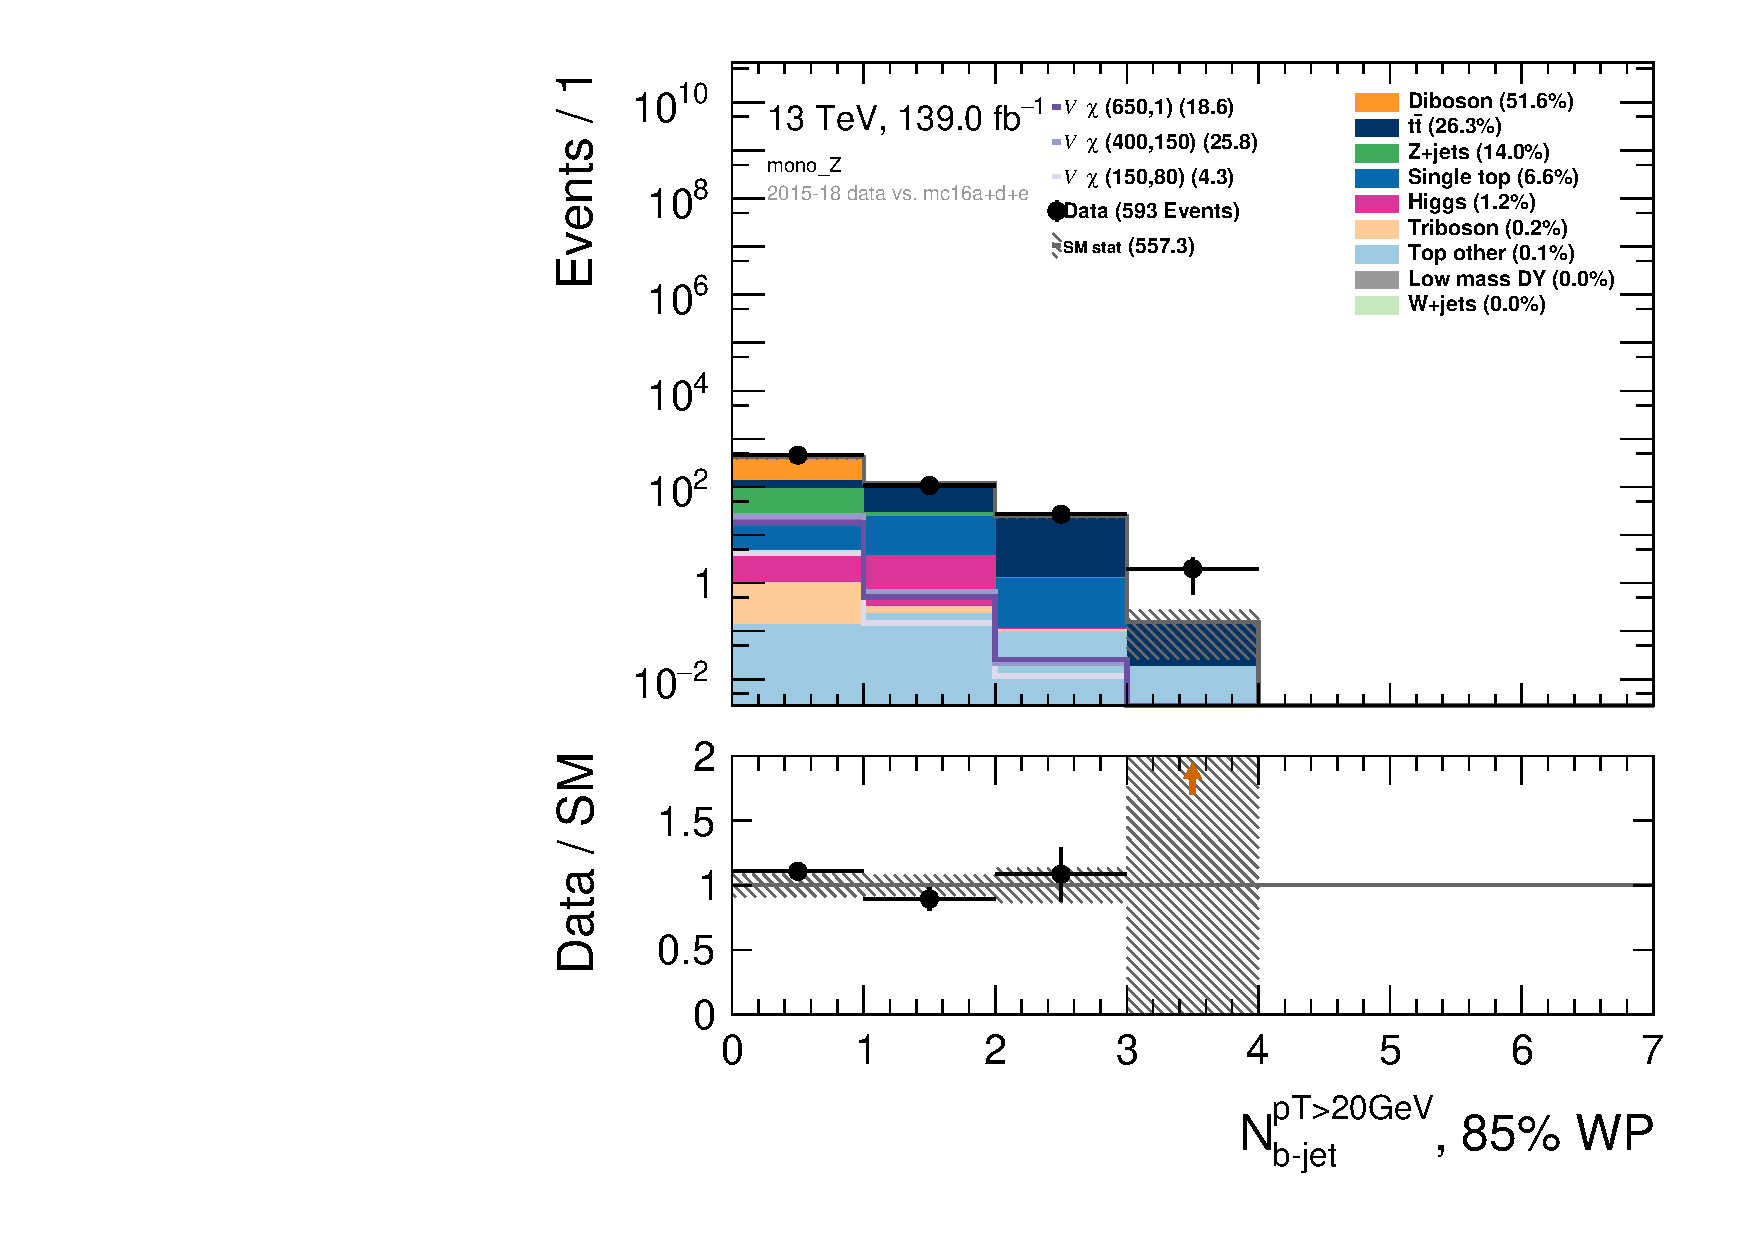
\includegraphics[width=\textwidth]{Figures/MonoZcuts/hist1d_nBJet20_MV2c10_FixedCutBEff_85_mono_Z.pdf}
    \caption{Stransverse mass for direct slepton production.}
    \label{fig:my_label}
    \end{subfigure}
    \begin{subfigure}[t!]{0.49\textwidth}
        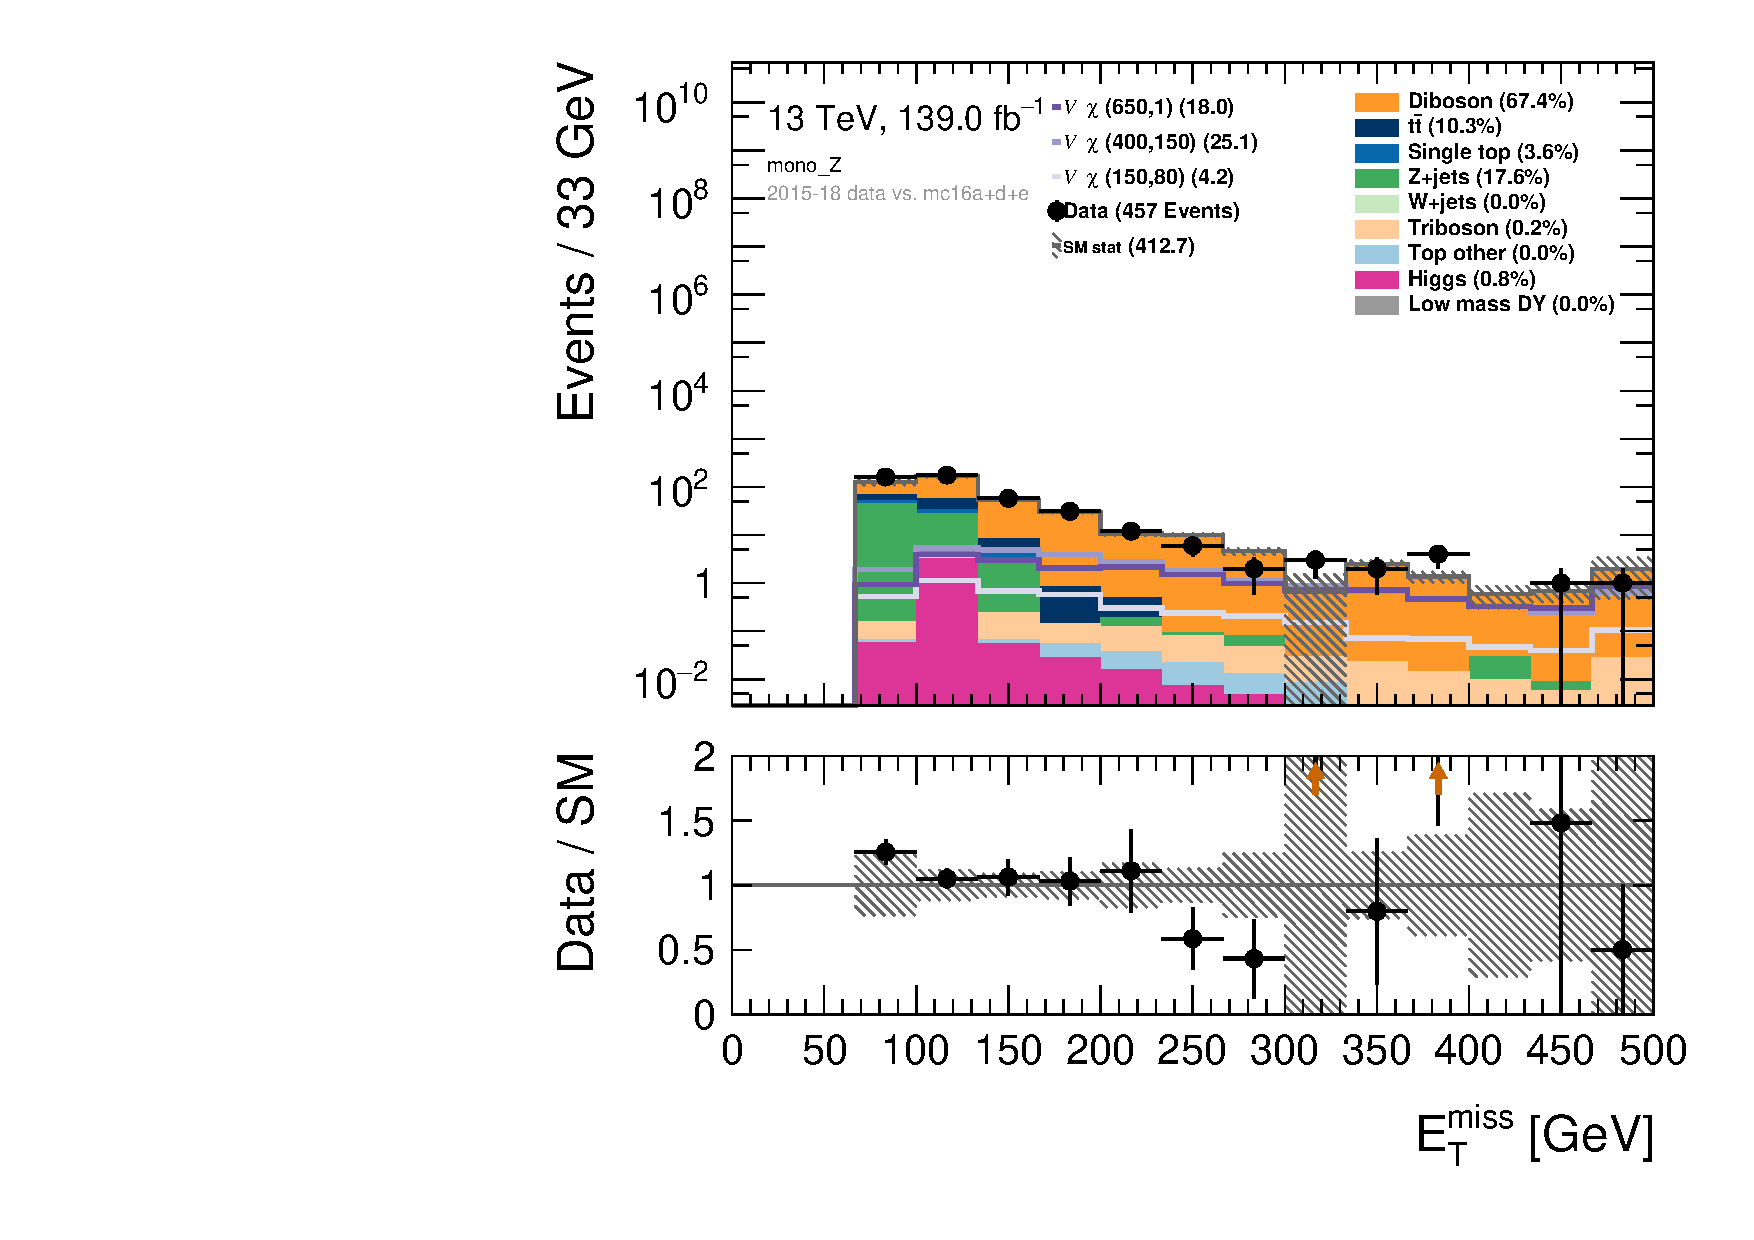
\includegraphics[width=\textwidth]{Figures/MonoZcuts/hist1d_met_Et_mono_Z.pdf}
    \caption{Stransverse mass for chargino production via $\Tilde{l}/\Tilde{\nu}$.}
    \label{fig:my_label}
    \end{subfigure}
    \caption{Plot of the four most important variables in direct slepton production with a cut on only two leptons with opposite charge in the final state.}
    \label{fig:cutandcountStepsDM}
\end{figure}
\restoregeometry
\end{comment}


All of the cuts are applied to get fewer background events while we, at the same time, do not want to cut away too much of the signal events. The publications have applied more or less the same cuts as listed above in table \ref{tab:cutsSUSY} and \ref{tab:cutsDM}, and their results are presented in figure \ref{fig:atlaspub}.


\begin{figure}[H]
\centering
    \begin{subfigure}[H]{0.49\textwidth}
        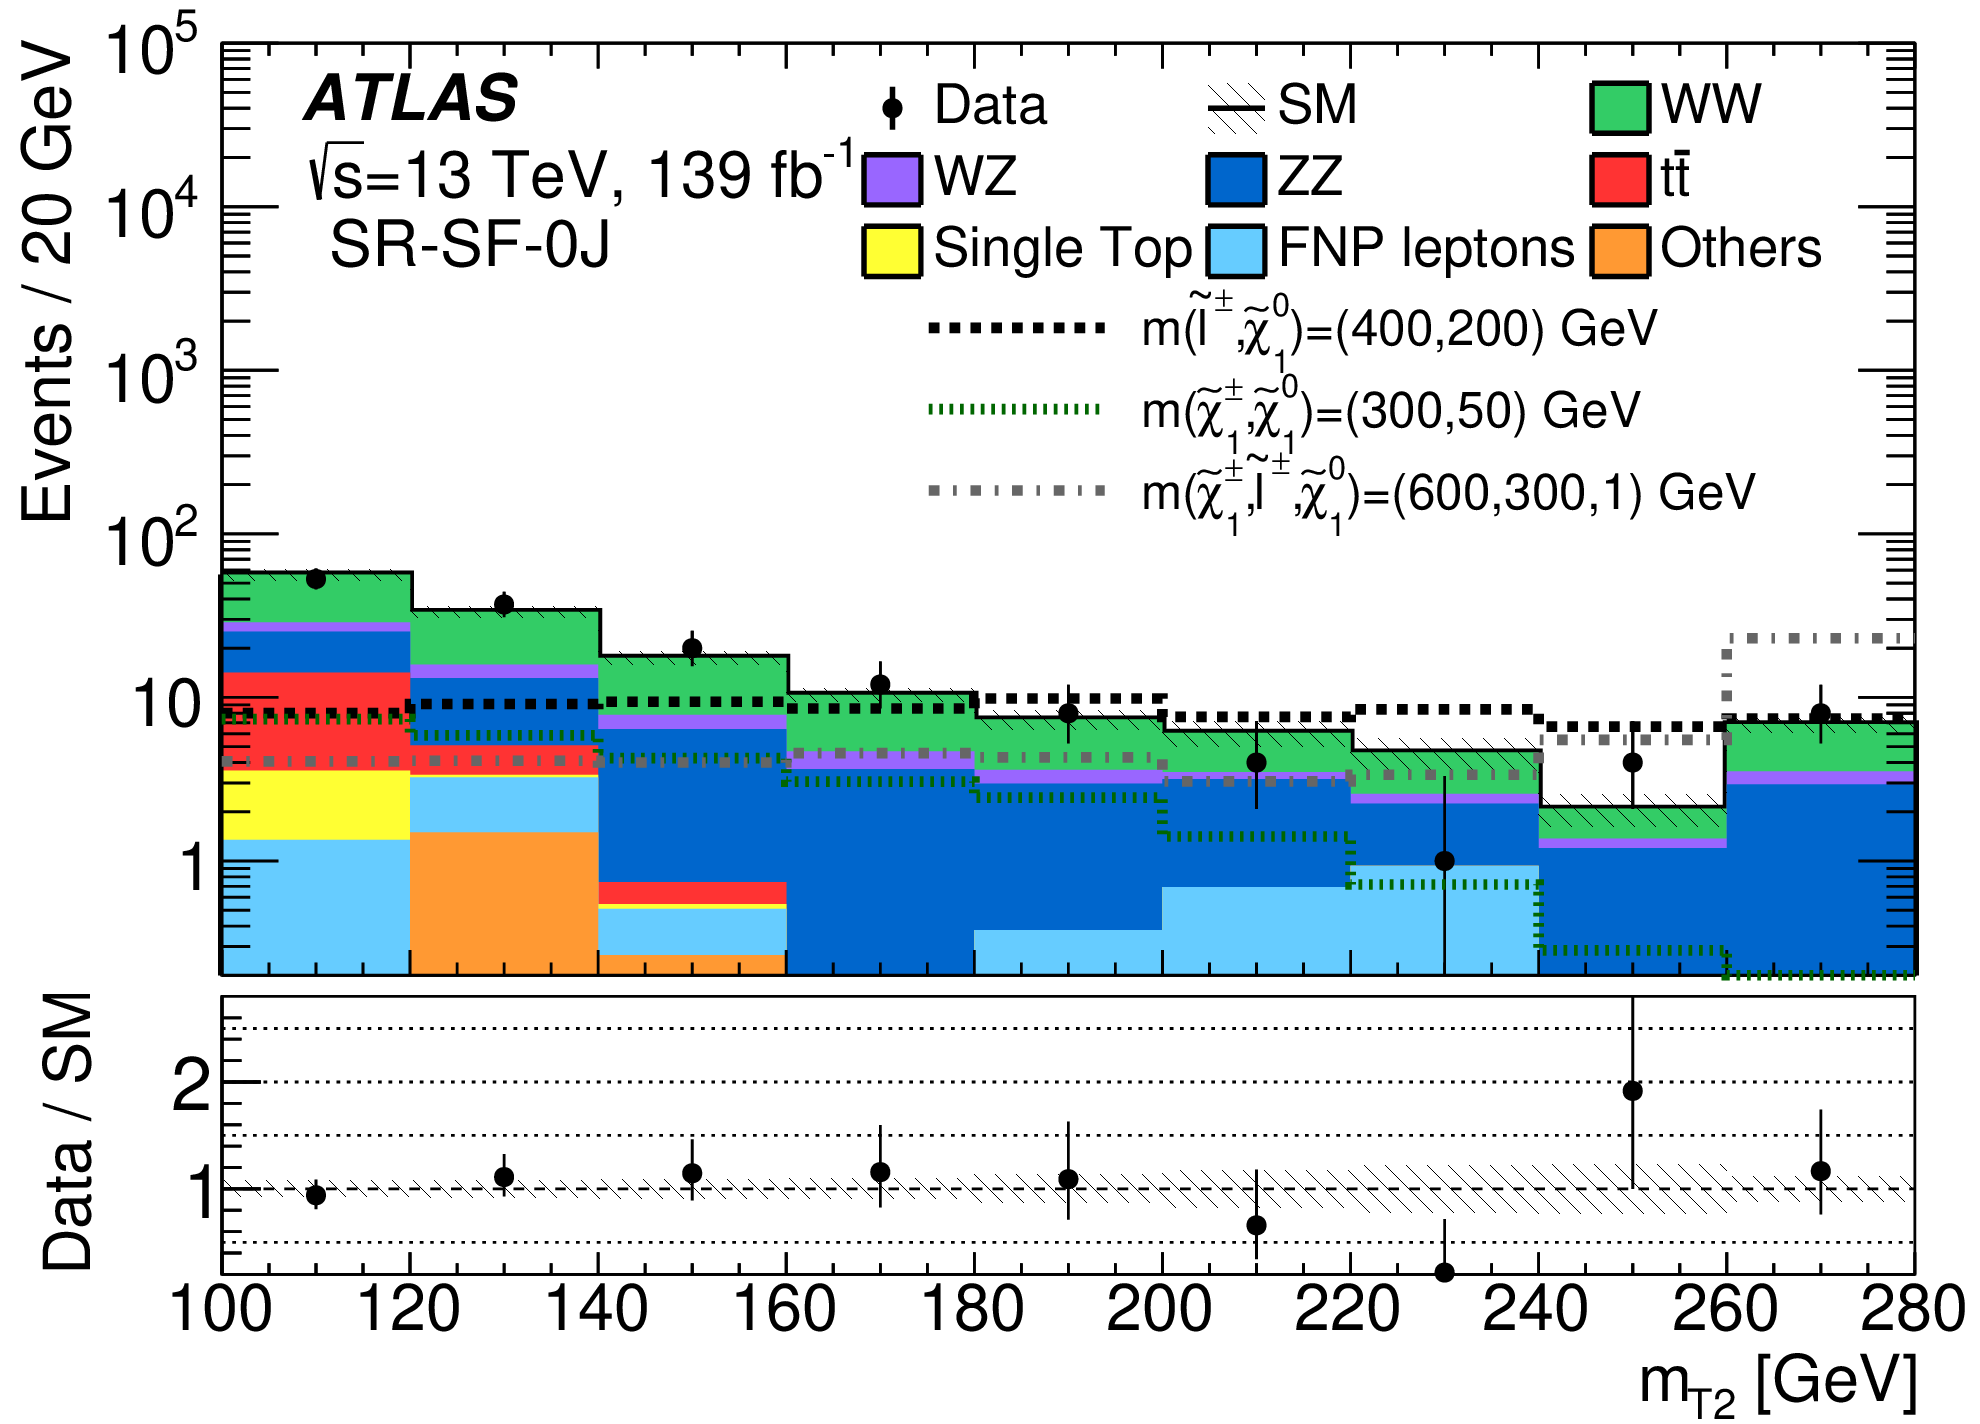
\includegraphics[width=\textwidth]{Figures/FromOnline/atlasmt2SUSY.png}
    \caption{Stransverse mass for direct slepton production, chargino production with $\Tilde{l}/\Tilde{\nu}$-mediated decays and with W-boson-mediated decays.}
    \label{fig:atlasSUSY}
    \end{subfigure}
    \\
    \begin{subfigure}[H]{\textwidth}
        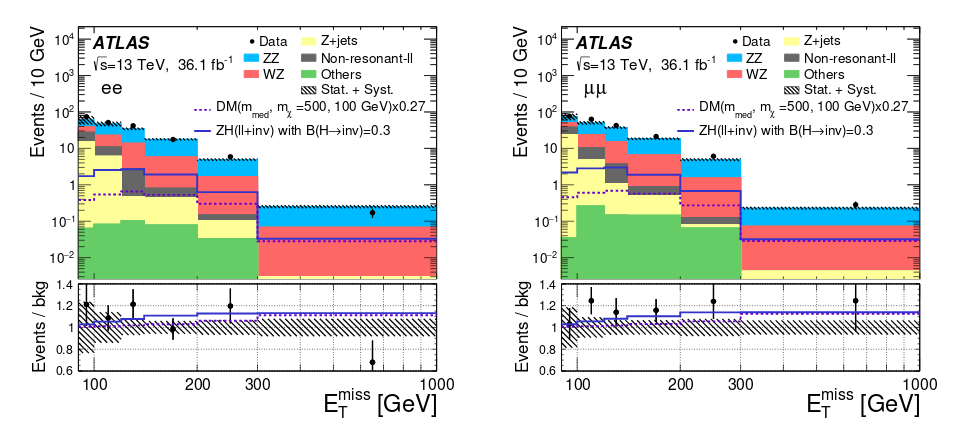
\includegraphics[width=\textwidth]{Figures/FromOnline/atlasmetDM.png}
    \caption{Missing transverse energy for the mono-Z process, where the left plot is the electron channel and right is the muon channel.}
    \label{fig:atlasDM}
    \end{subfigure}
    \caption{Results from the ATLAS publications for the four processes considered in this thesis.}
    \label{fig:atlaspub}
\end{figure}


In figure \ref{fig:atlasSUSY}, we can see that the signal is separated from the background for both the direct slepton production and the chargino production with W-boson-mediated-decay. However, they have not obtained any significant separation for chargino production with slepton/sneutrino-mediated-decay, which means that we should not expect to claim any discovery for the signal model shown in these plots. 

In figure \ref{fig:atlasDM}, we can see the plots for both electron channel and muon channel for the mono-Z process. It is not as much separation between signal and background as for the direct slepton production and the chargino production with W-boson-mediated-decay, but there is some. 

Later in this thesis, we will calculate the expected significance for the different processes we are looking at with both cut and count and ML. This is not done in the publications we are looking at, but they have included an exclusion plot which we can use for comparison later. This is shown in figure \ref{fig:exclusionPlots}. Here we can see the expected exclusion limit with $\pm1\sigma$ uncertainty bin together with the observed exclusion limit. The expected exclusion curve in these plots follow the boundary where the significance is 1.36 (i.e. 95\% CL exclusion). We are not going to reproduce these results in this thesis. However, we have used it to pick out some benchmark signals around the expected exclusion limit. 

\begin{figure}[H]
    \centering
    \begin{subfigure}[t!]{0.49\textwidth}
        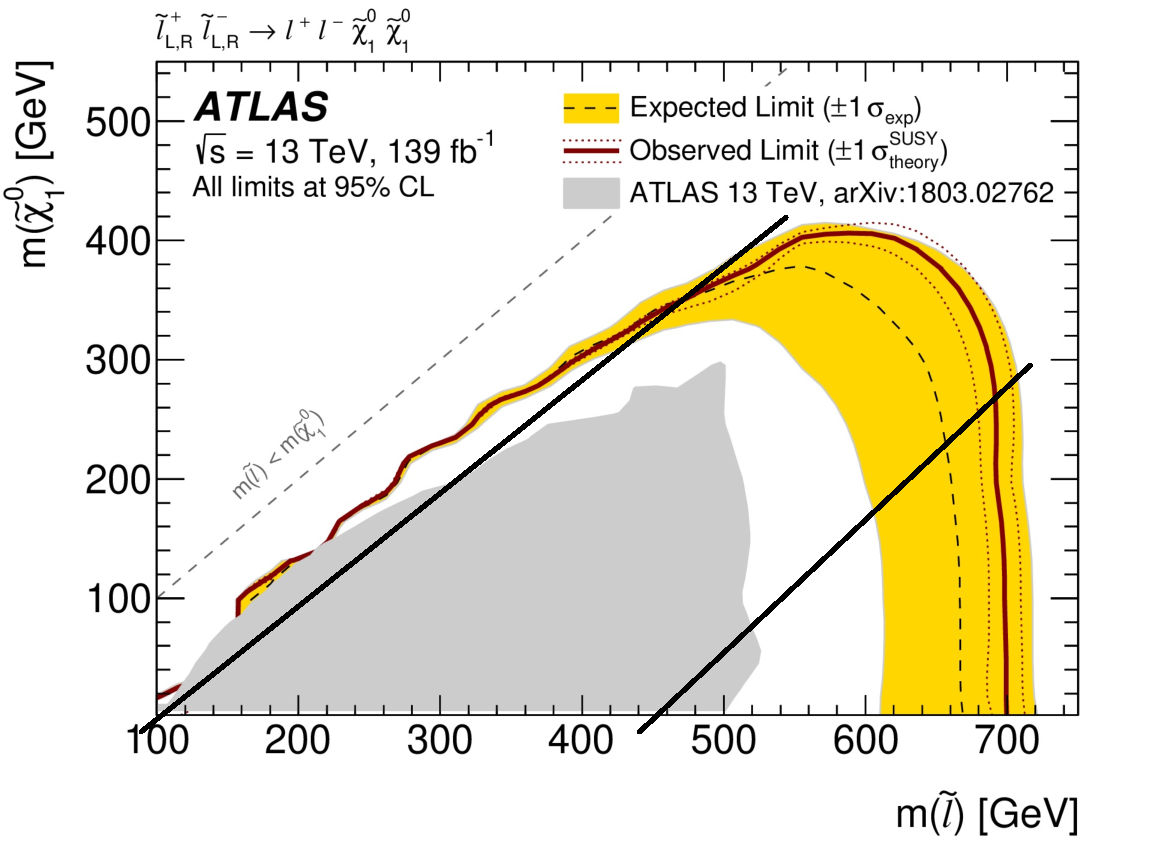
\includegraphics[width = \textwidth]{Figures/FromOnline/Slepslep.pdf}
        \caption{Slepton pair production ($\Tilde{l}\Tilde{l}$) \cite{sleptonexclusion}.}
        \label{fig:slepslepexclusion}
    \end{subfigure}
    \begin{subfigure}[t!]{0.49\textwidth}
        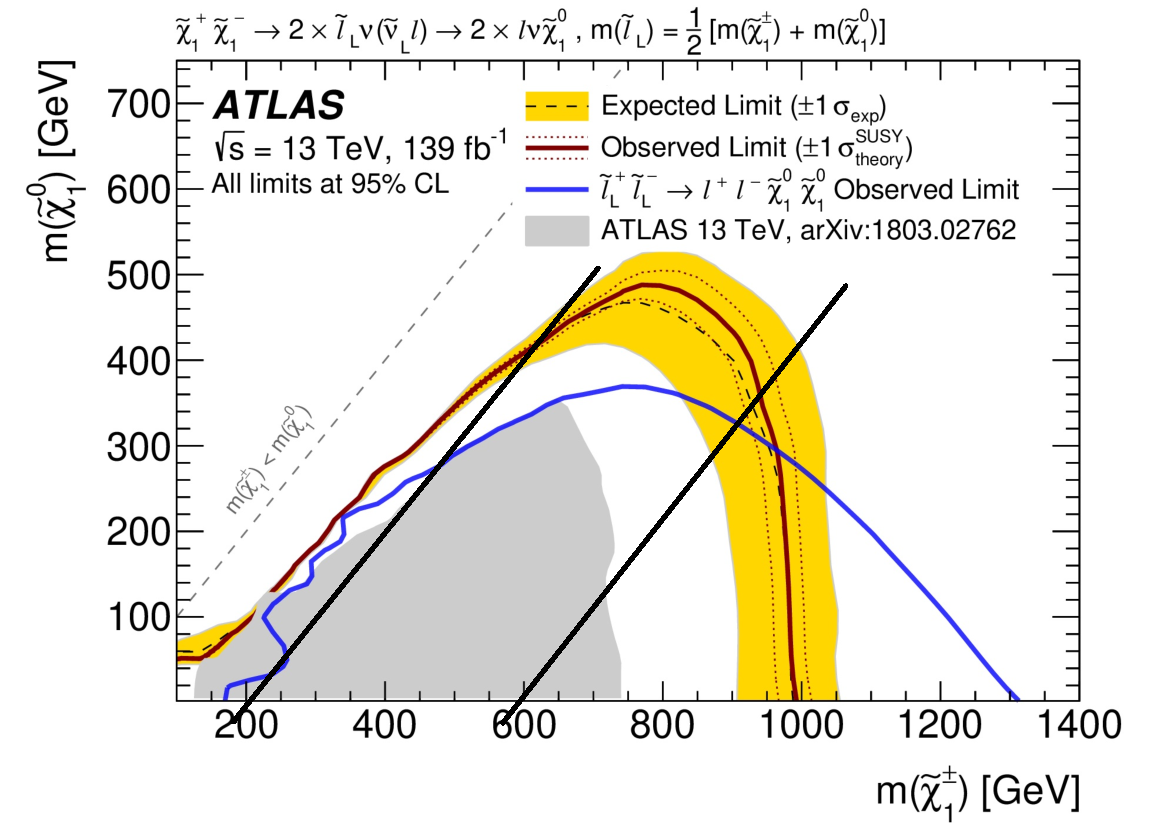
\includegraphics[width = \textwidth]{Figures/FromOnline/Slepsnu.pdf}
        \caption{$\chi_1^+ \chi_1^-$ production via $\Tilde{l}/\Tilde{\nu}$ \cite{sleptonexclusion}.}
        \label{fig:slepsnuexclusion}
    \end{subfigure}
    \\
    \begin{subfigure}[t!]{0.49\textwidth}
        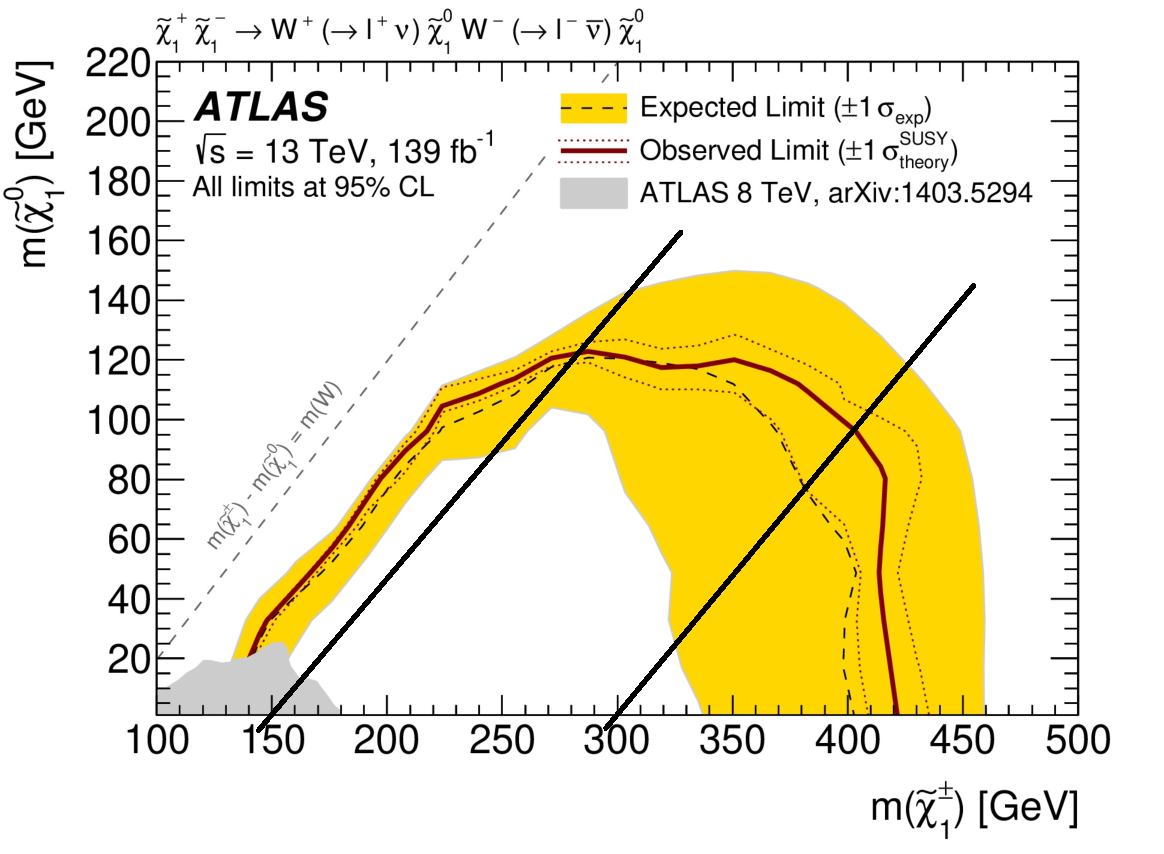
\includegraphics[width = \textwidth]{Figures/FromOnline/WW.pdf}
        \caption{$\chi_1^+ \chi_1^-$ production via W-boson \cite{sleptonexclusion}.}
        \label{fig:WWexclusion}
    \end{subfigure}
    \begin{subfigure}[t!]{0.49\textwidth}
        \includegraphics[width = \textwidth]{Figures/FromOnline/mono_Z.pdf}
        \caption{Mono-Z process \cite{monoZexclusion}.}
        \label{fig:monoZexclusion}
    \end{subfigure}
    \caption{The observed and expected exclusion limits for both the SUSY simplified models in \ref{fig:slepslepexclusion}, \ref{fig:slepsnuexclusion} and \ref{fig:WWexclusion} and for the DM model in \ref{fig:monoZexclusion}. The lines drawn in the plot is to show the mass splittings for each process.}
    \label{fig:exclusionPlots}
\end{figure}

The two black lines in each plot in figure \ref{fig:exclusionPlots} shows the division of the signal samples into different mass splittings in the ML analysis later in the thesis. To compare our ML results with the cut and count analysis, we have chosen one representative signal sample from each part of the plots in figure \ref{fig:exclusionPlots}. This gives us the signal samples listed in table \ref{tab:sigsampcutandcount}.

\begin{table}[H]
    \centering
    \begin{tabular}{c c c c}
    \toprule
    $\mathbf{(\Tilde{l}, \Tilde{\chi}_1^0)}$ & $\mathbf{(\Tilde{\chi}_1^\pm, \Tilde{\chi}_1^0)}$ & $\mathbf{(\Tilde{\chi}_1^\pm, \Tilde{\chi}_1^0)}$ & $\mathbf{( V, \chi)}$  \\
    \midrule
    \midrule
    (400, 300) & (300, 200) & (150, 25) & (150, 80)\\
    (600, 300) & (800, 400) & (350, 100) & (400, 150)\\
    (700, 1) & (1000, 100) & (425, 25) & (650, 1)\\
    \bottomrule
    \end{tabular}
    \caption{An overview of what signal samples that are used for this thesis.}
    \label{tab:sigsampcutandcount}
\end{table}

These signal samples are going to follow us through both analysis (cut and count and ML). They are also shown in figure \ref{fig:cutandcountMONA} where we have followed the same procedure as the ATLAS publications. The main difference between the publications and our results is that we have chosen some other signal samples than the publications. The publications have $m(\Tilde{l}, \Tilde{\chi}_1^0) = (400, 200)$ GeV, $m(\Tilde{\chi}_1^\pm, \Tilde{\chi}_1^0) = (300, 50)$ GeV, $m(\Tilde{\chi}_1^\pm, \Tilde{\chi}_1^0) = (600, 300)$ GeV and $m(V, \chi) = (500,100)$ GeV. Since we have chosen to look at different signal samples than the publications \cite{sleptonexclusion, monoZexclusion}, we have to see if the background for all four processes are compatible. 


In figure \ref{fig:cutandcountMONA} we can see our final results for the same variables as in the publications, from the cut and count analysis.

\newgeometry{twoside,inner=3cm,outer=2cm}
\begin{figure}[H]
%\begin{minipage}{2\textwidth}
%\begin{adjustwidth}{-3cm}{-3cm}
\centering
%\advance\leftskip-4cm 
%\advance\rightskip-4cm 
    \begin{subfigure}[t!]{0.49\textwidth}
        \includegraphics[width=\textwidth]{Figures/cutandcount/hist1d_mt2_direct_slepton.pdf}
    \caption{Stransverse mass for direct slepton production.}
    \label{fig:cutandcountslepslep}
    \end{subfigure}
    \begin{subfigure}[t!]{0.49\textwidth}
        \includegraphics[width=\textwidth]{Figures/cutandcount/hist1d_mt2_C1C1_SlepSnu.pdf}
    \caption{Stransverse mass for chargino production via $\Tilde{l}/\Tilde{\nu}$.}
    \label{fig:cutandcountslepsnu}
    \end{subfigure}
    \\
    \begin{subfigure}[t!]{0.49\textwidth}
        \includegraphics[width=\textwidth]{Figures/cutandcount/hist1d_mt2_C1C1_WW.pdf}
    \caption{Stransverse mass for chargino production via $W^\pm$.}
    \label{fig:cutandcountWW}
    \end{subfigure}
    \begin{subfigure}[t!]{0.49\textwidth}
        \includegraphics[width=\textwidth]{Figures/cutandcount/hist1d_met_Et_mono_Z.pdf}
    \caption{Missing transverse energy for mono-Z.}
    \label{fig:cutandcountmonoZ}
    \end{subfigure}
    \caption{Results from the cut and count analysis for all four processes, where we have followed the same procedure as the publications done by ATLAS.}
    \label{fig:cutandcountMONA}
\end{figure}
\restoregeometry


In figure \ref{fig:cutandcountMONA} we can see that for the direct slepton production and for the chargino production with slepton/sneutrino-mediated-decay we are able to separate some signal samples from the background in the high end of the $m_{T_2}$ variable. In \ref{fig:cutandcountslepslep} both the high and intermediate mass splitting samples are separated from the background and could lead to detection. In \ref{fig:cutandcountslepsnu} only the high mass splitting sample is above the background and could be possible to detect. While for the chargino production with W-boson-mediated-decay and mono-Z we have not been able to separate the signal from the background. In comparison to the results from the publications (shown in figure \ref{fig:atlaspub}), we can see that we have roughly the same amount of events in the different bins and can therefore conclude with that they are compatible and we have managed to reproduce the published results.

Now we are going to move on to the ML part, which is the main part of this thesis, and see if we can do the same analysis with some different tools. In the end we will compare the results obtained in this chapter to see if ML can do a better separation than we have manged to do with cut and count.


























\begin{comment}
%The first part of this analysis was done by cut and count. Here I have plotted four different variables which also represent some of the features used in the ML part. To demonstrate how the cut and count method behaves I have plotted each variable after adding a group of cuts. In the following figures you can see an example of this for the direct slepton production. You can also find examples of this for the charginos via slepton/sneutrino and via W-bosons in the appendix(OR GITHUB REPO??????). These two processes behave very similarly to the direct slepton production so I have chosen to show only one of them. 

%In the first figure \ref{fig:slepslep1stcut} we can see the whole mass distribution for the SM background with the final state two leptons with opposite charge. We can see that Z-jets is definitely the dominating background and by adding some cuts we can reduce this background.


\begin{figure}[H]
%\begin{minipage}{2\textwidth}
%\begin{adjustwidth}{-3cm}{-3cm}
\centering
%\advance\leftskip-4cm 
%\advance\rightskip-4cm 
    \begin{subfigure}[t!]{0.49\textwidth}
        \includegraphics[width=\textwidth]{Figures/SlepSlep/CutAndCount/1stcut_2L+OS/hist1d_mll_direct_slepton.pdf}
    \caption{Invariant mass}
    \label{fig:my_label}
    \end{subfigure}
    \begin{subfigure}[t!]{0.49\textwidth}
        \includegraphics[width=\textwidth]{Figures/SlepSlep/CutAndCount/1stcut_2L+OS/hist1d_met_Et_direct_slepton.pdf}
    \caption{Missing transverse energy}
    \label{fig:my_label}
    \end{subfigure}
    \\
    \begin{subfigure}[t!]{0.49\textwidth}
        \includegraphics[width=\textwidth]{Figures/SlepSlep/CutAndCount/1stcut_2L+OS/hist1d_mt2_direct_slepton.pdf}
    \caption{Stransverse mass}
    \label{fig:my_label}
    \end{subfigure}
    \begin{subfigure}[t!]{0.49\textwidth}
        \includegraphics[width=\textwidth]{Figures/SlepSlep/CutAndCount/1stcut_2L+OS/hist1d_met_Sign_direct_slepton.pdf}
    \caption{Missing transverse energy significance}
    \label{fig:my_label}
    \end{subfigure}
    \caption{Plot of the four most important variables in direct slepton production with a cut on only two leptons with opposite charge in the final state.}
    \label{fig:slepslep1stcut}
\end{figure}


After adding a met cut and doing a Z-veto we get the results in figure \ref{fig:slepslep3rdcut} where we can see that Z + jets is reduced a lot. For most of the variables we can now see that the $t\Bar{t}$ is the dominating background, but the signal is still below the backgrounds so we need to add some more cuts.

\begin{figure}[H]
%\begin{minipage}{2\textwidth}
%\begin{adjustwidth}{-3cm}{-3cm}
\centering
%\advance\leftskip-4cm 
%\advance\rightskip-4cm 
    \begin{subfigure}[t!]{0.49\textwidth}
        \includegraphics[width=\textwidth]{Figures/SlepSlep/CutAndCount/3rdcut_Zveto/hist1d_mll_direct_slepton.pdf}
    \caption{Invariant mass}
    \label{fig:my_label}
    \end{subfigure}
    \begin{subfigure}[t!]{0.49\textwidth}
        \includegraphics[width=\textwidth]{Figures/SlepSlep/CutAndCount/3rdcut_Zveto/hist1d_met_Et_direct_slepton.pdf}
    \caption{Missing transverse energy}
    \label{fig:my_label}
    \end{subfigure}
    \\
    \begin{subfigure}[t!]{0.49\textwidth}
        \includegraphics[width=\textwidth]{Figures/SlepSlep/CutAndCount/3rdcut_Zveto/hist1d_mt2_direct_slepton.pdf}
    \caption{Stransverse mass}
    \label{fig:my_label}
    \end{subfigure}
    \begin{subfigure}[t!]{0.49\textwidth}
        \includegraphics[width=\textwidth]{Figures/SlepSlep/CutAndCount/3rdcut_Zveto/hist1d_met_Sign_direct_slepton.pdf}
    \caption{Missing transverse energy significance}
    \label{fig:my_label}
    \end{subfigure}
    \caption{Plot of the four most important variables in direct slepton production with a cut on $E_T^{miss} >110$, $E_T^{miss}$ significance $>10$ and a Z-veto in addition to the previous cuts.}
    \label{fig:slepslep3rdcut}
\end{figure}



After adding some jet cuts (number of jets with $p_T$> 30GeV = 0 and a b-jet veto) we get the results in figure \ref{fig:slepslep4th_3_cut}. We can see that we succeeded on reducing the $t\Bar{t}$ background as well and we now have diboson as the dominating background.

\begin{figure}[H]
%\begin{minipage}{2\textwidth}
%\begin{adjustwidth}{-3cm}{-3cm}
\centering
%\advance\leftskip-4cm 
%\advance\rightskip-4cm 
    \begin{subfigure}[t!]{0.49\textwidth}
        \includegraphics[width=\textwidth]{Figures/SlepSlep/CutAndCount/4thcut_3_Bjets/hist1d_mll_direct_slepton.pdf}
    \caption{Invariant mass}
    \label{fig:my_label}
    \end{subfigure}
    \begin{subfigure}[t!]{0.49\textwidth}
        \includegraphics[width=\textwidth]{Figures/SlepSlep/CutAndCount/4thcut_3_Bjets/hist1d_met_Et_direct_slepton.pdf}
    \caption{Missing transverse energy}
    \label{fig:my_label}
    \end{subfigure}
    \\
    \begin{subfigure}[t!]{0.49\textwidth}
        \includegraphics[width=\textwidth]{Figures/SlepSlep/CutAndCount/4thcut_3_Bjets/hist1d_mt2_direct_slepton.pdf}
    \caption{Stransverse mass}
    \label{fig:my_label}
    \end{subfigure}
    \begin{subfigure}[t!]{0.49\textwidth}
        \includegraphics[width=\textwidth]{Figures/SlepSlep/CutAndCount/4thcut_3_Bjets/hist1d_met_Sign_direct_slepton.pdf}
    \caption{Missing transverse energy significance}
    \label{fig:my_label}
    \end{subfigure}
    \caption{Plot of the four most important variables in direct slepton production with a cut on number of jets and b-jets = 0 in addition to the previous cuts.}
    \label{fig:slepslep4th_3_cut}
\end{figure}

After adding one last cut in the $m_{T_2}$  variable we can see that the background doesn't change that much and that our signals is almost cut away as well. 

\begin{figure}[H]
%\begin{minipage}{2\textwidth}
%\begin{adjustwidth}{-3cm}{-3cm}
\centering
%\advance\leftskip-4cm 
%\advance\rightskip-4cm 
    \begin{subfigure}[t!]{0.49\textwidth}
        \includegraphics[width=\textwidth]{Figures/SlepSlep/CutAndCount/5thcut_1_mt2_100/hist1d_mll_direct_slepton.pdf}
    \caption{Invariant mass}
    \label{fig:my_label}
    \end{subfigure}
    \begin{subfigure}[t!]{0.49\textwidth}
        \includegraphics[width=\textwidth]{Figures/SlepSlep/CutAndCount/5thcut_1_mt2_100/hist1d_met_Et_direct_slepton.pdf}
    \caption{Missing transverse energy}
    \label{fig:my_label}
    \end{subfigure}
    \\
    \begin{subfigure}[t!]{0.49\textwidth}
        \includegraphics[width=\textwidth]{Figures/SlepSlep/CutAndCount/5thcut_1_mt2_100/hist1d_mt2_direct_slepton.pdf}
    \caption{Stransverse mass}
    \label{fig:my_label}
    \end{subfigure}
    \begin{subfigure}[t!]{0.49\textwidth}
        \includegraphics[width=\textwidth]{Figures/SlepSlep/CutAndCount/5thcut_1_mt2_100/hist1d_met_Sign_direct_slepton.pdf}
    \caption{Missing transverse energy significance}
    \label{fig:my_label}
    \end{subfigure}
    \caption{Plot of the four most important variables in direct slepton production with a cut on $m_{T_2} > 100$ GeV in addition to the previous cuts.}
    \label{fig:slepslep5th_1_cut}
\end{figure}


After adding all of the cuts mentioned above we can see that the signal almost no longer is present which is pretty bad when we want to see if the data follows the signal or the background. Since this isn't working that well, we are going to try to see if cuts found by ML is a better solution. 

\end{comment}















\begin{comment}


\begin{figure}[H]
%\begin{minipage}{2\textwidth}
%\begin{adjustwidth}{-3cm}{-3cm}
\centering
%\advance\leftskip-4cm 
%\advance\rightskip-4cm 
    \begin{subfigure}[t!]{0.49\textwidth}
        \includegraphics[width=\textwidth]{Figures/SlepSlep/CutAndCount/1stcut_2L+OS/hist1d_mll_direct_slepton.pdf}
%    \caption{Caption}
    \label{fig:my_label}
    \end{subfigure}
    \begin{subfigure}[t!]{0.49\textwidth}
        \includegraphics[width=\textwidth]{Figures/SlepSlep/CutAndCount/1stcut_2L+OS/hist1d_met_Et_direct_slepton.pdf}
 %   \caption{Caption}
    \label{fig:my_label}
    \end{subfigure}
    \\
    \begin{subfigure}[t!]{0.49\textwidth}
        \includegraphics[width=\textwidth]{Figures/SlepSlep/CutAndCount/1stcut_2L+OS/hist1d_mt2_direct_slepton.pdf}
  %  \caption{Caption}
    \label{fig:my_label}
    \end{subfigure}
    \begin{subfigure}[t!]{0.49\textwidth}
        \includegraphics[width=\textwidth]{Figures/SlepSlep/CutAndCount/1stcut_2L+OS/hist1d_nBJet20_MV2c10_FixedCutBEff_77_direct_slepton.pdf}
  %  \caption{Caption}
    \label{fig:my_label}
    \end{subfigure}
    \\
    \begin{subfigure}[t!]{0.49\textwidth}
        \includegraphics[width=\textwidth]{Figures/SlepSlep/CutAndCount/1stcut_2L+OS/hist1d_nJet20_direct_slepton.pdf}
%    \caption{Caption}
    \label{fig:my_label}
    \end{subfigure}
    \begin{subfigure}[t!]{0.49\textwidth}
        \includegraphics[width=\textwidth]{Figures/SlepSlep/CutAndCount/1stcut_2L+OS/hist1d_nJet30_direct_slepton.pdf}
 %   \caption{Caption}
    \label{fig:my_label}
    \end{subfigure}
\end{figure}

\begin{figure}[H]
%\begin{minipage}{2\textwidth}
%\begin{adjustwidth}{-3cm}{-3cm}
\centering
%\advance\leftskip-4cm 
%\advance\rightskip-4cm 
    \begin{subfigure}[t!]{0.49\textwidth}
        \includegraphics[width=\textwidth]{Figures/SlepSlep/CutAndCount/1stcut_2L+OS/hist1d_lepPt[0]_direct_slepton.pdf}
%    \caption{Caption}
    \label{fig:my_label}
    \end{subfigure}
    \begin{subfigure}[t!]{0.49\textwidth}
        \includegraphics[width=\textwidth]{Figures/SlepSlep/CutAndCount/1stcut_2L+OS/hist1d_lepPt[1]_direct_slepton.pdf}
 %   \caption{Caption}
    \\
    \label{fig:my_label}
    \end{subfigure}
    \begin{subfigure}[t!]{0.49\textwidth}
        \includegraphics[width=\textwidth]{Figures/SlepSlep/CutAndCount/1stcut_2L+OS/hist1d_lepPt_direct_slepton.pdf}
  %  \caption{Caption}
    \label{fig:my_label}
    \end{subfigure}
    \begin{subfigure}[t!]{0.49\textwidth}
        \includegraphics[width=\textwidth]{Figures/SlepSlep/CutAndCount/1stcut_2L+OS/hist1d_pTdiff_direct_slepton.pdf}
%    \caption{Caption}
    \\
    \label{fig:my_label}
    \end{subfigure}
    \begin{subfigure}[t!]{0.49\textwidth}
        \includegraphics[width=\textwidth]{Figures/SlepSlep/CutAndCount/1stcut_2L+OS/hist1d_deltaRll_direct_slepton.pdf}
 %   \caption{Caption}
    \label{fig:my_label}
    \end{subfigure}
    \begin{subfigure}[t!]{0.49\textwidth}
        \includegraphics[width=\textwidth]{Figures/SlepSlep/CutAndCount/1stcut_2L+OS/hist1d_deltaPhi_direct_slepton.pdf}
  %  \caption{Caption}
    \label{fig:my_label}
    \end{subfigure}
\end{figure}

\begin{figure}[H]
%\begin{minipage}{2\textwidth}
%\begin{adjustwidth}{-3cm}{-3cm}
\centering
    \begin{subfigure}[t!]{0.49\textwidth}
        \includegraphics[width=\textwidth]{Figures/SlepSlep/CutAndCount/1stcut_2L+OS/hist1d_met_HT_direct_slepton.pdf}
%    \caption{Caption}
    \label{fig:my_label}
    \end{subfigure}
    \begin{subfigure}[t!]{0.49\textwidth}
        \includegraphics[width=\textwidth]{Figures/SlepSlep/CutAndCount/1stcut_2L+OS/hist1d_HT_direct_slepton.pdf}
 %   \caption{Caption}
    \label{fig:my_label}
    \end{subfigure}
%\end{adjustwidth}
\end{figure}
\end{comment}






%



\chapter{Introducing Machine Learning}
%\label{sec:Methods}
\label{sec:ML}
In this chapter, we will get introduced to the different Machine Learning algorithms that are used in the analysis. 

The future of scientific experiments faces a problem: on the one hand, we have more data than we ever have in the history of science. It opens up a whole new range of possibilities and increases the potential for new findings. On the other hand, the quantity of data is so vast that no human being, or group of human beings, could hope to sift through and analyze all the data in a single lifetime. However, it's not good enough to have a ``dumb'' computer algorithm sort through the data, since if the computer cannot adapt and pick out interesting features, a human would need to double check the results anyway. We need a technique that is both efficient and ``smart''. For this reason, and others, Machine Learning (ML) is fast becoming the standard way of analyzing data in science, and in high energy physics in particular. 

Indeed, compared to the cut and count method, ML techniques are often a more efficient way to perform analyses. It can handle massive datasets and give results in a reasonable time frame. This is needed since the datasets have become increasingly large after each experimental upgrade at for e.g. the LHC. The ML methods are also usually more sensitive to the separation between the signal and the background (because it might pick out characteristics in the data that a human would never notice), which we are trying to optimize in our analysis. The regular cut and count analysis is performed by a person, and they analyze the data. For us, however, we will try to separate the signal from the background using ML algorithms. A discussion of these is presented in the following sections. 

Broadly speaking, a ML algorithm can be explained as shown in figure \ref{fig:MLex}. We have an input variable X that we send into an ML model of our choice, and we get the actual output Y (the ML output) and the predicted output Y' (the output we expect). Let us say that we give the ML model a variable with label 1; then the predicted value is 1 and the actual output will (hopefully) be either 1 or close to 1.   

\begin{figure}[H]
    \centering
    \includegraphics[width = \textwidth]{Figures/FromOnline/MLex.png}
    \caption{A very simple illustration of an ML algorithm \cite{MLex}.}
    \label{fig:MLex}
\end{figure}


\begin{comment}
In this thesis we are, as mentioned earlier, focusing on using ML algorithms to find new optimal cuts. This is just one of many ways of using ML in particle physics. Another way is to use it for anomaly detection of new particles. In that instance, we train our ML algorithm on background and then it will tell you if it have found something that is not behaving like the known backgrounds. \improvement{Dette hører kanskje heller hjemme i en evt outlook??}
\end{comment}


\section{Machine learning basics}
In this thesis, we are focusing on using ML algorithms to separate the signal from the background. This is done by the ML algorithms called Boosted Decision Trees (BDT) and Neural Networks (NN). Before we go into the specifics, we will give a short introduction to some ML basics.

\subsection{Training and testing}
\label{sec:TandT}
To obtain our BDT and NN results, we have to split our datasets into training and test sets. We split the dataset into 2/3 for training and 1/3 for testing. It is common practice to divide the train and test set like this, but it is also possible to choose a smaller training set and bigger test set. The reason for doing this is that we want to check if our model is learning and is able to classify the background as background and the signal as signal - before we, in the end, give it actual data. 

\subsubsection{Validation test}
In addition to a standard test set, we need a validation set to avoid overtraining (this is not used to test whether the model works, but rather to prevent overfitting - see below). A validation set is a set that hasn't been used to train the algorithm. We use the validation set to see when the model cannot do better with calculating a validation loss, which is the loss for the validation set - and will be explained later in this chapter - for each epoch or estimator the network or BDT goes through. An epoch is the number of cycles the NN does the training and estimator is the number of the times we want to boost the tree. If the validation loss does not become better after e.g., ten steps, another function breaks the training before it has finished all of the epochs or estimators. This is done by a function called \textit{early stopping}, which stops the training. This is very useful for the NN and BDT since there is one less parameter we have to worry about, namely the epochs or estimators. We only have to set a value high enough for the model to get far enough through the training. 

\subsection{Overfitting and underfitting}
In ML we encounter a very common problem while training our model, namely overfitting and underfitting. The goal when training a model is to get it to fit the data as well as possible; but this training can't be too precise or the the model will be useless if your data doesn't look exactly the same the next time you are using it. That would lead to loss of generality and our model would become dataset specific. This is overfitting. Underfitting is of course the opposite problem: the model is too simple to adapt to slightly more complex datasets, and the algorithm will simply use a simple function to fit data. These ideas are very well illustrated in figure \ref{fig:overunderfitting}. 

\begin{figure}[H]
    \centering
    \includegraphics[width = \textwidth]{Figures/FromOnline/overunderfitting.png}
    \caption{An illustration of underfitting and overfitting \cite{overunderfittingpic}.}
    \label{fig:overunderfitting}
\end{figure}



\subsection{Evaluating metrics}

\subsubsection{Accuracy}
In ML we have many ways to measure how well or badly our algorithm is performing; one of them is the \textit{accuracy} \cite{accuracy}. The accuracy expresses in percentage how accurate your algorithm is performing and can be calculated as

\begin{equation}
    \label{eq:acc}
    accuracy = \frac{correct}{correct + incorrect},
\end{equation}
where \textit{correct} is all data points that are classified as true positives (TP) and \textit{incorrect} as false positives (FP)\footnote{\textit{True positives} are all the datapoints that are correctly classified as positives, while \textit{false positives} are the datapoints that are classified as positive when they actually are negative. The same labeling holds for the negative classifications (TN/FN).}. This could be the only metric needed to evaluate a model; it gives a very basic measure of how, well, accurate - or reliable - the ML model is. 

\subsubsection{Loss and cost function}
Earlier we mentioned a validation loss, which also is calculated for the whole training set during training. The loss is calculated for each estimator (BDT) and epoch (NN). The loss can be calculated in many different ways and we should choose the one best suited for the problem. In our case we want to classify the background and signal as two variables, namely 0 and 1. This means that we are looking at a binary classification problem and we can use a binary classification loss function \cite{Loss}, namely binary \textit{cross-entropy}. Mathematically it can be derived as follows. We have a true probability $p_i$ and a distribution of the predicted values $q_i$. The probability to get the outcome $y=1$ is given by

\begin{equation}
    \label{eq:prob1}
    q_{y=1} = \Hat{y} = g(\textbf{w} \cdot \textbf{x}) = \frac{1}{1+e^{-\textbf{w} \cdot \textbf{x}}},
\end{equation}
where $\textbf{x}$ is a vector of input features, $\textbf{w}$ is a vector of optimized weights and $g(\textbf{w} \cdot \textbf{x})$ is a logistic function.

To find the probability of $y=0$ we can write

\begin{equation}
    \label{eq:prob0}
    q_{y=0} = 1- \Hat{y}.
\end{equation}

This gives us the notation setup, $p \in \{y, 1-y\}$ and $q \in \{\Hat{y}, 1-\Hat{y}\}$ and we can get the difference between $p$ and $q$ by using the cross-entropy $H(p,q)$, which leads to

\begin{equation}
    \label{eq:crossentropy}
    H(p,q) = - \sum_i p_i log q_i = - y log \Hat{y} - (1-y) log(1-\Hat{y})
\end{equation}

While we are training, logistic regression optimizes the log loss $J$\footnote{Here the loss function is called the cost function $J$. This might be a bit confusing because the cost function is defined ass the loss function for all training sets, but in our case the loss and cost are the same.} which means that we optimize the cross-entropy in the sample. This is given by

\begin{equation}
    \label{eq:loss}
    J(\textbf{w}) = \frac{1}{N} \sum_{n=1}^N H(p_n, q_n) = - \frac{1}{N} \sum_{n=1}^N \big[y_n log \Hat{y}_n + (1-y_n) log(1-\Hat{y}_n)\big],
\end{equation}
where $\Hat{y}_n$ is defined by equation \ref{eq:prob1}.

Cross-entropy is the best loss function to use in our case and is the preferred function to use in similar cases. Ideally, the cross-entropy loss should be 0 during training - this corresponds to the minimum possible loss. In practice, this does not happen; in fact, a validation loss of 0 normally indicates a different problem  - likely overfitting. 


\subsubsection{ROC-curve and AUC-score}
To analyze our results from both ML algorithms, we are going to use the ROC-curve and the AUC-score, which is short for Receiver Operating Characteristic and Area Under Curve. AUC refers to the area under a ROC curve, and this curve is a plot of the True Positive Rate (TPR) against the False Positive Rate(FPR). TPR is the actual positives that are identified correctly, called \textit{signal efficiency}, and FPR is the rate between the negative events categorized as positive and the negative events. In figure \ref{fig:ROCAUCex}, we can see how this looks. 

\begin{figure}[H]
    \centering
    \includegraphics[width = 0.5\textwidth]{Figures/FromOnline/ROCAUC.jpg}
    \caption{An example of a ROC curve \cite{ROCAUC}.}
    \label{fig:ROCAUCex}
\end{figure}

If we look at the green line in \ref{fig:ROCAUCex}, which is changing from model to model, we can see it has a smooth curve. If the green line creates a right angle in the top left corner, we will get an AUC score of 1, meaning the ML algorithm classifies correctly every signal and background event. In other words, the algorithm picks correctly every time. If the green line follows the diagonal dashed line, the algorithm is correct approximately 50 \% of the time, which is statistically the same as having the model randomly classify objects. If the curve is goes below the dashed line, the model classifies the background events as signal and the signal events as background, precisely the opposite of what we are trying to do. 










\begin{comment}
The use of machine learning (ML) is becoming the standard way of analysing data and interpreting various measurements and searches for new physics. ML is a more sophisticated method to do an analysis than the regular methods, such as the cut and count method. It is also usually more sensitive which gives us the opportunity to separate the signal from the background more efficiently than we do today.  We classify ML and specifically neural networks (NN) into two types, deep and shallow. Deep neural networks (DNN) is a NN with several hidden layers with quite few nodes/neurons in each layer. Shallow neural network (SNN) is a NN with only one hidden layer, but to obtain good results you need many more nodes/neurons in the hidden layer which gives us much more parameters to worry about. In this project we are going to concentrate on deep learning and compare the results with a simple SNN. 
\end{comment}


\section{Boosted Decision Trees}
\label{sec:BDT}

Boosted decision trees (BDT's) are one of the easiest ways to implement Machine Learning. It's typically not very sensitive to its hyperparameters, and is relatively easy to set up. In this thesis we have used XGBoost \cite{xgboostAbout}, which is one specific way to boost a decision tree. Before we explain boosted DTs however, we have to understand a regular DT.


\subsection{Decision Tree}

A decision tree is something we often do when thinking, even if we don't refer to the process as such. When we make a choice, we use a decision tree. Let us say that we have a picture of a person and we want to figure out if it is a boy or a girl. To make this conclusion we identify different features like whether the person has long hair, a beard, makeup, and so on. Then we set up a decision tree that will split our input data, which in this case is our picture, and make decisions based on the features you give it. Of course, we are not going to look on gender recognition in this thesis, but in principle decision trees can classify many things. This was just a small illustration of the simplicity and broad usage of BDT's.

Our goal is to use these principles to separate the signal from the background events. We give our decision tree some input data \cite{DTppt}, which consists of Monte Carlo (MC) simulated background and different signal samples (which are also obtained by MC simulations). Our decision tree will then split our data based on features we provide, e.g. invariant mass and missing transverse energy. 

\begin{figure}[H]
    \centering
    \includegraphics[width=0.5\textwidth]{Figures/FromOnline/Basic-structure-of-a-decision-tree-All-decision-trees-are-built-through-recursion.png}
    \caption{A sketch of how a decision tree is set up. \cite{DTpic}}
    \label{fig:DTpic}
\end{figure}

If we look at figure \ref{fig:DTpic}, we can see that we have three layers and three different types of nodes. The \textit{root node} is our input node, i.e. our input data, which for the first round is signal and background samples. Then the decision tree splits up our input data depending on the features we give it. This part will happen continuously through \textit{internal nodes} until we hit the depth of the tree, i.e. the last layer, or only have \textit{leaf nodes} left. As mentioned in section \ref{sec:TandT}, we split our input data into train and test parts where we save some data to test how well our model is trained. If we are happy with our results, we can test our pretrained model on real data and potentially extract some signal.


\subsection{Boosting}
Decision trees are weak learners (meaning that they typically perform badly), but if we ensemble several weak learners, we can get a strong learner. This process gives what it is called a boosted decision trees. Boosting creates a collection of predictors, which means that we fit consecutive trees, and at every step, we try to solve for the net error from the prior tree. If a hypothesis misclassifies the input, its weight will increase, so it would more likely classify it correctly next time. In figure \ref{fig:BDT}, we can see a sketched diagram of a BDT.


\begin{figure}[H]
    \centering
    \includegraphics[width = 0.7\textwidth]{Figures/FromOnline/BDT.png}
    \caption{Illustration of a BDT \cite{BDTpic}.}
    \label{fig:BDT}
\end{figure}

There are many ways to boost a decision tree, but in this thesis we have used a Python software library called XGBoost \cite{xgboostAbout}, which is short for eXtreme Gradient Boosting. This library uses a gradient descent while boosting the decision trees. The gradient descent is an algorithm that can optimize the differential loss function, i.e., the next tree will try to recover the loss from the previous tree. Note that the loss is defined as the difference between actual and predicted values \cite{BDT}. 

XGBoost is optimized to be highly efficient and flexible \cite{xgboostAbout}. It is written in C++, but offers a user interface in python and other languages. In this thesis we are using a class in XGBoost called \texttt{XGBClassifier} which, as implied by the name, classifies the data. We give all our input data a label 0 or 1 for background and signal respectively and train our model, with the different features, on what should have label 0 or 1 in the end. This is what we call \textit{supervised learning} because we help our model by providing a label in the input. The \texttt{XGBClassifier} takes a lot of arguments, which can be found in the Scikit-Learn API reference guide \cite{xgboostargument}, but in this thesis we use just the ones that are necessary for our purpose. The arguments that we have used are mentioned in the analysis chapter.

\subsection{Feature importance}
We are also going to look at the feature importance in the analysis. This is a way to see which features were important while constructing our BDT. This is an interesting aspect of the analysis because this will change from process to process and we will also be able to see if it matters if we train on different signal samples or not.

\section{Neural networks}
\label{sec:NN}
Neural Networks (NN) are probably the most popular machine learning algorithms that we use today. This is also what is often used for face and speech recognition by companies like Google and Apple \cite{NNarticle}. NN does basically the same as a BDT, but instead of splitting the input data into background and signal at each node, each node is trained on different features. 

NN are a collection of nodes, like the ones we have in BDT. \ref{sec:BDT}. Instead of many trees with nodes, we are now creating a network with these nodes as we can see in figure \ref{fig:NN}. 


\begin{figure}[H]
    \centering
    \includegraphics[width = 0.5\textwidth]{Figures/FromOnline/tikz35.png}
    \caption{Illustration of a neural network \cite{NNpic}.}
    \label{fig:NN}
\end{figure}

We can see that the network consists of one input layer, one hidden layer and one output layer. This is a very simple NN and is often called a \textit{shallow neural network} (SNN) since it has only one hidden layer. If we increase the number of hidden layers to two or more we have a deep neural network (DNN) as we can see in figure \ref{fig:DNN}

\begin{figure}[H]
    \centering
    \includegraphics[width = 0.7\textwidth]{Figures/FromOnline/tikz36.png}
    \caption{Illustration of a deep neural network \cite{NNpic}.}
    \label{fig:DNN}
\end{figure}

In this thesis we have built a NN with a tool called \texttt{KerasClassifier}\footnote{Keras \cite{keras} is a NN library for Python.} which, as for the BDT, classifies the data. For our network to be able classify, we have to send in some pre-labeled data to train it. This is done by simply giving the background label 0 and signal label 1. Additionally, we have to understand what happens in the NN to know what parameters we should adjust in order to train and analyse the data. 

The NN has many more dependencies than the BDT. It is therefore unfortunately more sensitive to possible under- and overtraining, but for correct composition of parameters, it will typically be better trained than a BDT. To achieve the optimal results, we need a lot of computing power and time to optimize. 

There are many advantages and disadvantages with both SNN and DNN but it is in principle possible to achieve the same results with both. In a SNN you can increase the number of nodes and get the same results as for a DNN with several layers and fewer nodes in each layer. The problem with doing it that way is that we get more free parameters by increasing the number of nodes, which again increases the possibility that our model gets biased and hence over or underfits.

This is unfortunately not as trivial as for a BDT, but maybe easier to adapt to different purposes. In our case we are going to use it to distinguish signal from background.

With the basics in place, we can now describe NNs in more detail. Next we provide an overview of the activation function, how the network evolves, and how it gets better with training.

\subsection{Activation functions}
To get the output for the different nodes in a layer, we need an activation function. This output is again used as input for the next layer until you reach the last layer, which then will give us our final output/results.

Since Machine Learning doesn't come from a theoretical prediction which is implemented numerically, the choice of activation function for different problems is found by trial and error. The activation function will provide a number between 0 and 1 \cite{AF}, which is sent into the next nodes in the next layer. Some activation functions provide a number between -1 and 1 instead, but this depends on how the activation function we choose behaves, as we can see in figure \ref{fig:activations}. In the next sections we are going to look more closely at the different activation functions we have used in this thesis. We are also going to consider some other activation functions that are not used in this thesis but still of very common use in ML.


%In the network, each node uses an activation function to send the total input in that node as a number between 0 and 1 to the next layer. Tanh gives a number between -1 and 1.

\begin{figure}[H]
    \centering
    \begin{subfigure}[t!]{0.3\textwidth}
    \includegraphics[width=\textwidth]{Figures/sigmoid.pdf}
    \caption{}
    \label{fig:sigmoid}
    \end{subfigure}
    \begin{subfigure}[t!]{0.3\textwidth}
    \includegraphics[width=\textwidth]{Figures/tanh.pdf}
    \caption{}
    \label{fig:tanh}
    \end{subfigure}
    \begin{subfigure}[t!]{0.3\textwidth}
    \includegraphics[width=\textwidth]{Figures/relu.pdf}
    \caption{}
    \label{fig:relu}
    \end{subfigure}
    \caption{This is an illustration of the behaviour of three different activation functions. In (a) we can see the Sigmoid function, in (b) the Tanh function, and in (c) the ReLU function.}
    \label{fig:activations}
\end{figure}



\textbf{Sigmoid}

The Sigmoid function, figure \ref{fig:sigmoid}, is a logistic activation function and is given by equation \ref{eq:sigmoid} below.

\begin{equation}
    \label{eq:sigmoid}
    a_i = \frac{1}{1+e^{(-z_i)}},
\end{equation}

where $z_i$ is the output value from the i-th node in the output layer.

As we can see in figure \ref{fig:sigmoid}, the Sigmoid function gives us a value between 0 and 1. This makes this activation function a good choice if we have to predict a probability for the output. A drawback, and the reason we have to use other activation functions sometimes, is that the Sigmoid can get the NN stuck on its training time because of the calculation time of the exponential. This is not an optimal activation function to use inside the network, but in the output layer it is the preferred one. We want our network to classify our output as signal or background which we have labeled as 1 and 0. 


\textbf{Tanh (Hyperbolic tangent)}

In addition to the Sigmoid function we have the tanh function, figure \ref{fig:tanh}, which is shaped the same way as the Sigmoid function, but it gives values between -1 and 1 instead of between 0 and 1. This we can see in figure \ref{fig:tanh} and it is given by equation \ref{eq:tanh} below.

\begin{equation}
\label{eq:tanh}
a_i = \tanh(z_i)
\end{equation}

Since we also can get negative numbers from this activation function, it is preferred instead of the Sigmoid if we have negative numbers in the input. This function returns negative values as negative unlike e.g. Sigmoid which only returns 0 or 1. Since we don't care for negative values in our case, this activation function is not used in this thesis. 

\textbf{ReLU (Rectified Linear Unit)}

One of the most popular activation functions is the ReLU function. This function outputs 0 for any negative value, and if the value is positive, the function returns the value as it is. This is shown in figure \ref{fig:relu}. Since all data that is below zero becomes zero, it can be hard do get a good read out of the data because the data may sometimes assume negative values. The ReLU function is given by equation \ref{eq:relu}.

\begin{equation}
\label{eq:relu}
    a_i = max(0,z_i).
\end{equation}

Since we're not interested in negative values we are using this activation function in our hidden layers. The Sigmoid function would also be a good choice when we are thinking about our wanted form of the output. But, as mentioned earlier, it can get stuck in its training time.

\textbf{Other activation functions}

The three functions mentioned above are not the only activation functions one can use. Since every problem has different approaches, we have to adjust these functions for our needs. There are, for example, many different adjustments done with the ReLU function to get a better activation output in problems that need adjustment to perform optimally. One of the newest activation functions is called Swish \cite{Swish}, which is simply a modification of the Sigmoid function given by equation \ref{eq:swish}. 

\begin{equation}
    \label{eq:swish}
    a(x) = x \cdot Sigmoid(x)
\end{equation}

The developers of the Swish function state that it does overall a better job than the widely used ReLU function, but until this time there is no evidence in literature supporting this claim. As such, we will stick with ReLU in this thesis. 

\subsection{Feed forward and back propagation} 
Every node in the neural network has an activation function connected to itself and if the node is connected to another node it also has a weight for each node it is connected to. To create the new node we simply multiply the nodes activation with the weight and sum them together like so

\begin{equation}
    a_1 \cdot w_1 + .. + a_n \cdot w_n = \text{new node}
\end{equation}

This operation is done for every node in every layer, and fed to the next layer until we hit the the output layer. This is what we call \textit{feed forward} because we always send the obtained information forward from input to output layer.

We also have a method to go back in the network to optimize it, namely \textit{back propagation}. What we do is go back to the previous layers to optimize the weights. This is not what we call an optimizer and should not be confused with that; it's merely the process of going backwards. Back propagation is probably the most important step in a NN, because this optimizes our model and makes sure that our training goes well. 

\subsection{Optimizers}

When training a NN, we need to know how well it performs during and after the training. For this we use a loss function $L$. There are many different types of functions that are used, depending on what we want to do with the network.

We want to minimize the loss function to make the prediction error as small as possible, i.e. optimize the network. And to do this, we use an optimizer.

\subsubsection{Stochastic Gradient Descent\cite{training_model}}

The gradient descent method uses the fact that a function $F(x)$, where $x = (x_1,x_2,...,x_n)$, will increase fastest in the direction of the gradient of the function, $\nabla F$. We want to move in the opposite direction of the gradient to make sure that we decrease the loss function.

We then multiply this gradient with a number $\eta$ called "the learning rate", and subtract this from the current weights $w_j$. In the case of neural networks, $F(x)$ is the loss function $L$. This leads to equation \ref{eq:w_update} 

\begin{equation}
    w_j = w_j - \eta\frac{\partial L}{\partial w_j}
    \label{eq:w_update}
\end{equation}

To speed up the training we can also add a stochastic part to the method, which means that we randomly choose a batch size of the data that we use to approximate the derivative, and use that to update the weights. This is also called Mini Batch Gradient Descent. 

The data that we want to use might be very noisy, so we can use a technique to de-noise the data \cite{SGD_momentum}. This is done by adding a momentum, which is a moving average of our gradients. We now subtract this from the weights. The equations now become 

\begin{equation}
    V_i = \beta V_i + (1 - \beta)\nabla_w L
    w_i = w_i - \eta V_i
    \label{eq:momentum}
\end{equation}

One way to look at this last addition is viewing the movement in parameter space as an object that moves one step at a time downhill. When we add momentum, it is like giving this object some physical momentum. Now when the object finds the minimum, it will continue a little bit back and forth to make sure it has found the minimum. A good reason to add this is if there are many saddle-points where the optimizer might stop. With momentum, it will move past, and then continue the descent on the other side without stopping.

\subsubsection{Adam\cite{Goodfellow-et-al-2016}}

The learning rate is one of the most difficult parameters to optimize, because any change to its value may have a huge impact on a method's performance. To circumvent this, we can use a method that has an adaptive learning rate. 

Adam is currently the most popular optimization algorithm today, and the name is derived from Adaptive Moments. It is an update to another optimization algorithm called RMSProp, which stands for Root Mean Square Propagation. RMSProp uses the running average of recent gradient magnitudes, and divides the learning rate by this average. This is done for every weight in the NN.

Adam takes this a step further. It uses an estimation of the first-order moments of the gradient as momentum, and also adds a bias correction to both the momentum and the second-order moments.



%\section{Quantifying the sensitivity}
\label{sec:significance}

The overall goal with the analysis carried out in this thesis is to optimize the sensitivity to discover new physics and possibly in the end to claim discovery of new particles. To check if we have succeeded in making our model sensitive to new physics we can check the expected p-values and significances for our signal region. 

Each event in the data will either pass or fail the cuts defining the signal region used in the analysis. The number of events therefore follows a binomial distribution, and the probability of finding $n$ events in our region is given by equation \ref{eq:pval1}. 

\begin{equation}
    \label{eq:pval1}
    P(n|N, p) = \frac{N!}{n!(N-n)!} p^n(1-p)^{N-n},
\end{equation}

where $N$ is the number of total events and p is the probability for the event to pass the cuts. If the number of total events gets very big and the probability $p$ gets very small, we can approximate equation \ref{eq:pval1} as a Poisson distribution, which is given by

\begin{equation}
    \label{eq:pval2}
    P(n|\nu) = \frac{\nu^n}{n!} e^{-\nu},
\end{equation}

where $\nu$ is given by a hypothesis. This equation (eq. \ref{eq:pval2}) gives us a probability of $n$ observed events when the expectation is to observe $\nu$ events. 

When we are talking about hypotheses in this thesis, we are talking about \textit{background-only} (b-only) and \textit{signal + background} (s+b) hypotheses. The b-only hypothesis is the SM, which is a well known theory. We are going to check this against the s+b hypothesis which in our case will be one of the three SUSY processes or the mono-Z process. This gives us the opportunity to introduce the p-values. A p-value is a measure to judge the deviation of the observed number of events from the b-only hypothesis expectations. If we assume that only the SM processes contribute we can use the p-value to get the probability of observing as many, or more, events as we can find in the data. With a perfectly known background the p-value can be found by

\begin{equation}
    \label{eq:pvalues}
    p = \sum_{n=n_{obs}}^\infty f(n;b),
\end{equation}


where $f(n;b)$ is the Poisson distribution given in equation \ref{eq:pval2}. It is common to convert the p-value into an observed significance $z$ with a unit Gaussian $\Phi$. This is given by

\begin{equation}
    \label{eq:signifobs}
    z = \Phi^{-1}(1-p)
\end{equation}

 and the unit is expressed with a $\sigma$ as in number of standard deviations from the center of the Gaussian distribution. To claim discovery of a new particle we need an observed significance above 5 $\sigma$. We are not going to check the observed significance in this thesis, but calculate the expected significance to see if there is any hope to discover new physics for the models we are looking at. The expected significance is the significance associated with the median number of expected events under the s+b hypothesis. It gives us a number on how well the two hypotheses we are looking at are separated. This is given by equation \ref{eq:signif}, where the p-value now is expressed as a \textit{confidence level} (CL) given as
 
 \begin{equation}
    \label{eq:CL}
    CL_{s+b} = \sum_{n=0}^{q_{obs}} \frac{(s+b)^n}{n!} e^{-(s+b)},
 \end{equation}

where $q_{obs}$ is the number of observed events. If the $CL_{s+b}$ is below 5\% we exclude that we can find any new physics with the selection criteria we have given it. Putting equation \ref{eq:signifobs} and \ref{eq:CL} together we get the expression

\begin{equation}
    \label{eq:signif}
    Z_N = \Phi^{-1}(1-CL_{s+b}),
\end{equation}

where $Z_N$ is the expected significance. To claim exclusion in the signal region we need a $CL_{s+b} \leq$ 5\% which corresponds to $Z_N \leq 1.64 \sigma$. In this thesis the $Z_N$ is calculated by an already existing tool in ROOT called \texttt{RooStats.NumberCountingUtils.BinomialExpZ} which simply takes the number of events for both background and signal as input together with a fractional background uncertainty of e.g. 20\%.







\begin{comment}

\begin{equation}
    \label{eq:pval3}
    p = P(n \geq q_{obs}|b) \sum_{n=q_{obs}}^\infty \frac{b^n}{n!} e^{-b}
\end{equation}

As mentioned several times in this project the goal is to claim discovery of the Higgs boson. To do that we have to reject the b-only hypothesis. To do this we are going to use p-values and confidence levels. \\


which is a probability of finding $n$ events in our signal region. 









\textbf{P-values}\\
Assuming a null hypothesis to be true we can use the p-value as a function that quantifies how often we would obtain data as far away from the null hypothesis as the observed data. Since it is a function of the data, the p-value is of course a random variable. We have the p-values $p_0$ and $p_1$ for the hypotheses $H_0$ and $H_1$ which is given by 

\begin{equation}
    \label{eq:p0}
    p_0 = \int_{t_{obs}}^{+ \infty} g(t|H_0) dt,
\end{equation}
and
\begin{equation}
    \label{eq:p1}
    p_1 = \int_{t_{obs}}^{+ \infty} g(t|H_1) dt.
\end{equation}

These are probabilities to find the test statistic ($t$) values that are equal or greater than the observed test statistic ($t_{obs}$). The p-values can also be expressed by confidence levels as

\begin{equation}
    \label{eq:p0CL}
    p_0 = 1-CL_b
\end{equation}
and 
\begin{equation}
    \label{eq:p1CL}
    p_1 = CL_{s+b}.
\end{equation}

How to calculate the $CL_b$ and $CL_{s+b}$ is shown in equation \ref{eq:CLb} and \ref{eq:CLsb} later in this section.\\

\textbf{Confidence levels}\\
The method we are using to check if this is a good fit is confidence levels. The confidence level tells us how often the results will fit the expectations. E.g. a confidence level of 90\% tells us that the results fit the expectations 90\% of the time. In figure \ref{fig:CL} we can see an illustrative plot of the test statistic distribution with the confidence levels marked. 


\begin{figure}[H]
    \centering
    \includegraphics[width = 0.7\textwidth]{Figures/CL.png}
    \caption{This is a illustration of the test statistic distribution for the b-only and s+b hypotheses with the $CL_b$ and $CL_{s+b}$ marked. \cite{datanal}}
    \label{fig:CL}
\end{figure}

The compability of the observed test statistic, $t_{obs}$, with the two hypothesis, b-only and s+b, are defined as

\begin{equation}
    \label{eq:CLb}
    1 - CL_b = \int_{-\infty}^{t_{obs}} \text{g(t; b-only) dt}
\end{equation}

and

\begin{equation}
    \label{eq:CLsb}
    CL_{s+b} = \int_{t_{obs}}^{+\infty} \text{g(t; s+b) dt}.
\end{equation}



\textbf{Results for the p-values and confidence levels}\\
By using equation \ref{eq:CLb} and \ref{eq:CLsb} we get the following results



In table \ref{tab:CLZ} we can see the results for the p-values ($1-CL_b$) and the confidence levels. As we can see is the expected significance is below 5$\sigma$ so we did not expect to claim a discovery which also is compatible with the observed significance from the data. \\

We can also see that the value for $CL_{s+b}$ for the b-only hypothesis is below 0.05 which is the limit for excluding this hypothesis but since the observed value is $> 0.05$ we can't exclude it either.  



\begin{table}[H]
    \centering
    \begin{tabular}{c c c}\hline
     & 1-CL_b & CL_{s+b}\\\hline\hline
    b-only     &  & \\
    s+b     &  &\\
    data &  & \\\hline
    \end{tabular}
    \caption{Caption}
    \label{tab:CL}
\end{table}


\begin{table}[H]
    \centering
    \begin{tabular}{c c}\hline
     & CL$_{s+b}$ \\\hline\hline
    Median s+b experiment     &  0.500\\
    Median b-only experiment     & 0.023\\
    Data & 0.843\\\hline
    \end{tabular}
    \caption{Caption}
    \label{tab:my_label}
\end{table}


\end{comment}
%%\chapter{Analysis}
\label{sec:Analysis}


%\chapter{Search for Supersymmetry and Dark Matter in Events with Dileptons and Missing Energy}
\label{sec:CandCanalysis}

%Beskriv prosessene her istedet for i teori og motiver hvordan partiklene er produsert. 

This chapter will introduce the processes we are searching for in the analysis, how the signal and background samples are produced, and how we do a traditional analysis when searching for new particles or phenomena in LHC data. We will show the results obtained by the ATLAS collaboration and compare the results with ours. 



The processes we are interested in looking at in this thesis involve superpartners of leptons, gauge bosons, and the Higgs boson. Besides this, we will look at a dark matter particle candidate, which is predicted to be the lightest supersymmetric particle (LSP).  This thesis looks at proton-proton collisions with final state two leptons and missing transverse energy (MET/$E_T^{miss}$). The SUSY processes we are looking at are direct slepton production, chargino production with slepton/sneutrino-mediated-decays and with W-boson-mediated-decays. 


In figure \ref{fig:SlepSlepFeynman} below, we can see the direct slepton production as a production of two hypothetical sleptons which decay to the final state, comprising of two leptons and missing transverse energy (i.e. missing energy in the detector). The neutralinos, which are the MET in this process, are a mixture of the sparticles photino, zino, and higgsino and is also one of the dark matter candidates mentioned above.  
\begin{figure}[H]
    \centering
    \includegraphics[width = 0.4\textwidth]{Figures/FeynmanDiagrams/SlepSlepFeynman.png}
    \caption{Direct slepton production $pp \rightarrow \tilde{l}^+ \tilde{l}^- \rightarrow l^+l^- + \tilde{\chi}_1^0 \tilde{\chi}_1^0$.}
    \label{fig:SlepSlepFeynman}
\end{figure}

In figure \ref{fig:SlepSnuFeynman} and \ref{fig:WWFeynman} we can see the chargino production with  slepton/sneutrino-mediated-decays and with W-boson-mediated-decays. Charginos are a mixture of the sparticles wino and the charged higgsino. These processes have the same final state as direct slepton production, but here the neutrinos are also a part of the MET, since we can't actually detect them in the detector. 
\begin{figure}[H]
    \centering
    \includegraphics[width = 0.4\textwidth]{Figures/FeynmanDiagrams/SlepSnuFeynman.png}
    \caption{Chargino production with slepton/sneutrino-mediated-decays $pp \rightarrow \tilde{\chi}_1^+ \tilde{\chi}_1^- \rightarrow \tilde{l}^+ \tilde{l}^- /\tilde{\nu} \tilde{\nu} \rightarrow l^+l^- + \nu \Bar{\nu} + \tilde{\chi}_1^0 \tilde{\chi}_1^0$.}
    \label{fig:SlepSnuFeynman}
\end{figure}

\begin{figure}[H]
    \centering
    \includegraphics[width = 0.4\textwidth]{Figures/FeynmanDiagrams/WWFeynman.png}
    \caption{Chargino production with W-boson-mediated-decays $pp \rightarrow \tilde{\chi}_1^+ \tilde{\chi}_1^- \rightarrow W^+ W^- \rightarrow l^+l^- + \nu \Bar{\nu} + \tilde{\chi}_1^0 \tilde{\chi}_1^0$.}
    \label{fig:WWFeynman}
\end{figure}

The DM process we are looking at in this thesis is the mono-Z process shown in figure \ref{fig:monoZFeynman2}. Here we have a mediator V which decays into the DM particles $\chi$ and a W/Z that decays into two leptons. This gives us the same final state as we had for the SUSY processes.  

\begin{figure}[H]
    \centering
    \includegraphics[width = 0.4\textwidth]{Figures/FeynmanDiagrams/monoZFeynman2.png}
    \caption{Mono-Z process $pp \rightarrow Z + MET \rightarrow l^+ l^- + MET$.}
    \label{fig:monoZFeynman2}
\end{figure}


\section{MC simulated events}

The data taken into consideration is from the ATLAS experiment at LHC between 2015-2018 (Run 2), further explained in chapter \ref{sec:LHCandATLAS}. But, we are also looking at some MC simulated background and signal which will be explained in this section. The explanations are taken from the publications from ATLAS, namely \cite{sleptonexclusion} for the SUSY signals and \cite{monoZexclusion} for the mono-Z signal. We present an overview of what signal samples that are used in table \ref{tab:directslepLOW} - \ref{tab:MonoZHigh} in section \ref{sec:sigsamptab}. 

The SUSY signal samples were generated from leading-order (LO) matrix elements with up to two extra partons using \textsc{MadGraph5\_aMC@NLO 2.6.1} \cite{48} interfaced to \textsc{Pythia 8.186} \cite{49}, with the A14 tune \cite{50}, for the modelling of the SUSY decay chain, parton showering, hadronisation and the description of the underlying event. Parton luminosities were provided by the NNPDF2.3LO PDF set \cite{51}. Jet–parton matching was performed following the CKKW-L prescription \cite{52}, with a matching scale set to one quarter of the mass of the pair-produced SUSY particles. Signal cross-sections were calculated to next-to-leading order (NLO) in $\alpha_s$ adding the resummation of soft gluon emission at next-to-leading-logarithm accuracy(NLO+NLL) \cite{53,54,55,56,57,58,59}. The nominal cross-sections and their uncertainties were taken from an envelope of cross-section predictions using different PDF sets and factorisation and renormalisation scales, as described in Ref. \cite{60}. 


To study the invisible Higgs boson decays, Monte Carlo events are produced for the SM ZH process with a subsequent Z boson decay into a dilepton pair and the H$\rightarrow$ZZ$\rightarrow \nu \nu \nu \nu$ decay (ZH$\rightarrow ll$+inv). The ZH signal processes from both the quark–antiquark (qqZH) and gluon–gluon (ggZH) initial states are modelled with \textsc{Powheg-Box v2} \cite{49Z, 50Z} using the CT10 \cite{51Z} parton distribution function (PDF) and interfaced to \textsc{Pythia8.186} \cite{52Z} for parton showering. The kinematic distributions of ZH$\rightarrow ll$ +inv events are described at next-to-leading-order (NLO) in QCD. Additionally, for the qqZH process, the MINLO \cite{53Z} method is applied to improve the gluon resummation calculation, and the $p_T^Z$ distribution is corrected to NLO electroweak (EW) accuracy with a reweighting approach detailed in Ref. \cite{3Z}. The SM ZH production cross-section is computed with next-to-next-to-leading-order (NNLO) QCD and NLO EW precision and found to be 884 fb \cite{3Z} with $m_H = 125$ GeV at 13 TeV. The DM signal is modelled with the leading-order \textsc{MadGraph5\_aMC@NLO} matrix element \cite{54Z} using NNPDF3.0 \cite{55Z} and showered with Pythia8.186. DM signal events with an axial-vector mediator and fermionic WIMPs are produced for different $m_{med}$ and $m_\chi$, both in a range from 10 to 1000 GeV.  As recommended in Ref. \cite{44Z}, the DM events are generated by choosing $g_q = 0.25$, $g_\chi = 1$, and a minimal mediator width. The AZNLO \cite{56Z} and A14 \cite{57Z} parameter sets are used to tune the \textsc{Pythia8.186} parton-shower for the simulation of the ZH $\rightarrow ll$+inv and DM signals, respectively.


The different backgrounds that we are considering are diboson, triboson, $t\Bar{t}$, single top, other top events ($t\Bar{t}$ events with a pair of leptons or boson(s)), Higgs, Drell-Yan, Z+jets and W+jets. The MC samples are simulated using different generators that are listed up in table \ref{tab:bkg_samples}. The goal is to separate these backgrounds from the signals we are looking at, which consist in the four different processes that we looked at earlier in this chapter. 

\begin{table}[H]
    \centering
    \begin{tabular}{l l l l} \toprule
        \textbf{Background sample} & \textbf{Generator} & \textbf{Parton shower} & \textbf{Normalisation}\\
        \midrule
        \midrule
        Diboson & \textsc{Sherpa2.2.2}\cite{sherpa2_1, sherpa1_2, sherpa1_3} & \textsc{Sherpa2.2.2} & NLO \cite{NLO}\\
        Triboson & \textsc{Sherpa2.2.2} & \textsc{Sherpa2.2.2} & NLO \\
        Z+jets & \textsc{Sherpa2.2.1} \cite{sherpa1_1, sherpa1_2, sherpa1_3} & \textsc{Sherpa2.2.1} & NNLO \cite{NNLO}\\
        W+jets & \textsc{Powheg-Box v2}\cite{49Z, 50Z} & \textsc{Pythia8.186} \cite{49} & NLO\\
        Drell-Yan & \textsc{Sherpa2.2.1} & \textsc{Sherpa2.2.1} & NNLO\\
        $t\Bar{t}$ & \textsc{Powheg-Box v2} & \textsc{Pythia8.186} & NNLO\\
        Single top & \textsc{Powheg-Box v2} & \textsc{Pythia8.186} & NLO\\
        topOther & \textsc{MG5\_aMC@NLO} \cite{48} & \textsc{Pythia8.186} & NLO\\
        Higgs & \textsc{Powheg-Box v2} & \textsc{Pyhtia8.186} & NLO\\
        \bottomrule
    \end{tabular}
    \caption{An overview of the different generators used to simulate the MC background samples.}
    \label{tab:bkg_samples}
\end{table}


Before we move on to how we perform the analysis, we also need to know how we are going to know that we see SUSY and DM particles in the detector. Since they never have been discovered, we have to lean on some hypotheses on how this is happening. As for all events in the detector, we have to reconstruct the events using their decays. The supersymmetric particles are expected to decay into cascades that will contain a LSP which will interact very weakly with the detector material which again will result in a big measured MET in the detector. The rest of the cascade will result in a final state with with leptons and/or jets. Together with the MET this gives us the final state we are looking for. For the mono-Z process we can measure the MET from the DM particles decayed from the unknown hypothetical mediator particle. Together with the leptons we get from the decay of the Z-boson, this gives us the same final state as for the SUSY processes.




































\begin{comment}

\begin{itemize}
    \item Bruker noe som eksisterer
    \item Tradisjonell måte ting har blitt gjort på
    \item begrenset av menneskets forståelse av prosessen vi ser på
    \item vi må bestemme alle kuttene som blir gjort
    \item Du må vite hva du skal se etter for å gjøre dette, altså trenger en teori/hypotese
    \item Tenk overgang til ML
    \item Valg må være begrunnet 
    \item Massesplitting. Cut and count er svak på lav massesplitting. Dette gjør ML bedre
\end{itemize}
\end{comment}








\section{The standard way: cut and count}
\label{sec:candc}

The first part of the analysis done in this thesis is a traditional cut and count analysis. \textit{Cut and count} is probably the most known method used in particle physics and has proved to be very useful in the discoveries we have done so far. Since the data become more and more massive and the processes we are looking at more and more complicated, we also need to develop further the way we perform the analysis. In this thesis, we are mainly going to focus on machine learning algorithms. Therefore we have not done much with this standard way to analyze and have based the cut and count on already published analyses from ATLAS \cite{sleptonexclusion, monoZexclusion}. 

In cut and count, we select events sensitive to new physics, i.e., we remove events which are not interesting for the signal process we consider. After applying several cuts, the selection of events we are left with form the so-called \textit{signal region}. We then see whether the expected signal is significantly separated from the expected Standard Model (SM) background in this region. We can calculate an expected significance $Z$, which will be explained in section \ref{sec:significance} later in the thesis, to check if we can expect to claim a discovery in this region if a particular signal model turns out to be realized in nature. If we are lucky and have cut away enough background and kept sufficient signal, we can check if the observed events in data are compatible with the signal+background hypothesis or if they match the background-only hypothesis (i.e. no signal) instead. Let us consider the case where the data differ from the background and tends to follow the signal: we know that there is most likely something interesting in this region.

Of course, there are advantages and disadvantages with every method, and this is also the case for cut and count. In cut and count, we need a theory or hypothesis as a reference to know what kind of signals we should look for. It is therefore unfortunately limited by the human understanding of what we are looking at. The lack of human understanding is where Machine Learning (ML) comes to help. The ML methods help us separate the signal from the background. This is further explained in the following chapters, where we will look at what the different ML methods do.






\section{Reproducing the ATLAS publications}
The first part of this analysis was done by cut and count and the goal was to reproduce the results from publications done by ATLAS \cite{sleptonexclusion, monoZexclusion}. Here we will compare our results to the official results from the ATLAS experiment, and hopefully achieve a good agreement between the two.

Since the goal is to reproduce the results, we implement more or less the same analysis procedure as described in the publications. The cuts done for the SUSY processes are listed in table \ref{tab:cutsSUSY} and for the mono-Z process in table \ref{tab:cutsDM}, where both tables are taken from the publications \cite{sleptonexclusion, monoZexclusion}. All the kinematic variables we cut on are presented in chapter \ref{sec:LHCandATLAS}. The first cut we do for both processes is to demand exactly two leptons with opposite signs in the final state.


\begin{table}[H]
    \centering
    \begin{tabular}{l l}\toprule
    \textbf{Variables} & \textbf{Cuts}\\
    \midrule
    \midrule
    Two leptons & Same flavor (SF) and opposite sign (OS)\\
    $n_{\text{non-b-tagged jets}}$     & 0 \\
    $m_{ll}$ [GeV]     & 121.2\\
    $E_T^{miss}$ [GeV] & $>$ 110 \\
    $E_T^{miss}$ significance & $>$ 10\\
    $n_{\text{b-tagged jets}}$ & 0\\
    $m_{T2}$ [GeV] & 160\\
    \bottomrule
    \end{tabular}
    \caption{Cuts added in the cut and count analysis taken from the publication for the SUSY processes \cite{sleptonexclusion}.}
    \label{tab:cutsSUSY}
\end{table}

For the SUSY processes we have applied the cuts in table \ref{tab:cutsSUSY}, where we, in addition to having only two leptons with opposite sign in the final state, demand that they have to have the same flavor as well. Here we get the Z+jets as the dominating background as we can see in both figure \ref{fig:nJetSUSY} and table \ref{tab:cutflowSUSY}. Now we want to reduce all of the background, especially Z+jets, and we apply the next cut in table \ref{tab:cutsSUSY} which is demanding no jets. As we can see in figure \ref{fig:mllSUSY}, the Z+jets background is still the dominating background, but if we look at table \ref{tab:cutflowSUSY}, we can see that it is reduced a lot. The reason for Z+jets is still dominating is that the jet-cut reduced around the same percentage from all of the different backgrounds. 

\begin{figure}[H]
\centering
    \begin{subfigure}[t!]{0.49\textwidth}
        \includegraphics[width=\textwidth]{Figures/SUSYcuts/hist1d_nJet20_SUSY.pdf}
    \caption{Number of jets with a $p_T > 20$ GeV.}
    \label{fig:nJetSUSY}
    \end{subfigure}
    \begin{subfigure}[t!]{0.49\textwidth}
        \includegraphics[width=\textwidth]{Figures/SUSYcuts/hist1d_mll_SUSY.pdf}
    \caption{The invariant mass of the two leptons.}
    \label{fig:mllSUSY}
    \end{subfigure}
    \caption{Plot of different distributions after applying the cuts on 2L, SF, OS and no jets.}
    \label{fig:stepsSUSY1}
\end{figure}


The next cut we have applied is on the invariant mass of the two leptons in the final state. The results are shown in figure \ref{fig:metSUSY} and as we can see, all of the background is reduced a lot. It is also done a cut requiring large missing transverse energy. This is done because it cuts away more background than signal, which entails obtaining a more significant separation between the signal and background. By applying this cut, we can see that the Z+jets are no longer the dominating background and the results are shown in figure \ref{fig:metSignSUSY} and table \ref{tab:cutflowSUSY}. 

\begin{figure}[H]
    \centering
    \begin{subfigure}[t!]{0.49\textwidth}
        \includegraphics[width=\textwidth]{Figures/SUSYcuts/hist1d_met_Et_SUSY.pdf}
    \caption{Missing transverse energy.}
    \label{fig:metSUSY}
    \end{subfigure}
    \begin{subfigure}[t!]{0.49\textwidth}
        \includegraphics[width=\textwidth]{Figures/SUSYcuts/hist1d_met_Sign_SUSY.pdf}
    \caption{Missing transverse energy significance.}
    \label{fig:metSignSUSY}
    \end{subfigure}
    \caption{Plot of different distributions after applying the cuts on the invariant mass and MET.}
    \label{fig:stepsSUSY2}
\end{figure}


The last three cuts applied is a cut on the MET significance, b-tagged jets and $m_{T2}$. The results after applying the MET significance cut is shown in figure \ref{fig:bjetSUSY} and as we can see, the diboson is still the dominating background. The second last cut that was done is to demand events with non b-tagged jets which do not reduce anything because we already have demanded no jets at all. This we can see in figure \ref{fig:mt2SUSY} and table \ref{tab:cutflowSUSY}. The last cut that are applied for the SUSY processes are on the $m_{T2}$ variable. This is done to get rid of the rest of the $t\Bar{t}$ background and leave us more or less with only diboson. This is part of our final result and are shown in figure \ref{fig:cutandcountMONA} later in this section.

\begin{figure}[H]
    \centering
    \begin{subfigure}[t!]{0.49\textwidth}
        \includegraphics[width=\textwidth]{Figures/SUSYcuts/hist1d_nBJet20_MV2c10_FixedCutBEff_85_SUSY.pdf}
    \caption{Number of b-tagget jets.}
    \label{fig:bjetSUSY}
    \end{subfigure}
    \begin{subfigure}[t!]{0.49\textwidth}
        \includegraphics[width=\textwidth]{Figures/SUSYcuts/hist1d_mt2_SUSY.pdf}
    \caption{Stransverse mass.}
    \label{fig:mt2SUSY}
    \end{subfigure}
    \caption{Plot of different distributions after applying the cuts on MET significance and b-jets.}
    \label{fig:stepsSUSY3}
\end{figure}

As we can see in figure \ref{fig:stepsSUSY1}-\ref{fig:stepsSUSY3} and table \ref{tab:cutflowSUSY}, the signal have been reduced, but not as much as all of the background contributions. This implies that we have been able to get rid of the background without affecting the signal too much, which also was our goal by doing this. 

\begin{landscape}
\begin{table}[H]
    \centering
    %\rotatebox{90}{
    \begin{tabular}{l l l l l l l l}
    \toprule
    \textbf{Sample} & \textbf{OS+SF+2L} & \textbf{jet-veto} & $\mathbf{m_{ll}}$ & \textbf{MET} & \textbf{MET sign} & \textbf{b-jets} & $\mathbf{m_{T_2}}$\\
    \midrule
    \midrule
        Drell-Yan & 733055.427 & 64177.536 & 40.384 & 0.000 & 0.000 & 0.000 & 0.000 \\
        Higgs & 1055360.610 & 442535.035 & 451.966 & 3.222 & 2.411 & 2.411 & 0.005\\
        Single top & 96745.087 & 7383.056 & 3313.872 & 283.960 & 174.644 & 174.644 & 0.000\\
        $t\Bar{t}$ & 948716.615 & 16272.119 & 7648.974 & 710.246 & 340.903 & 340.903 & 0.000\\
        Z+jets & 142460122.600 & 97803688.386 & 1273912.476 & 533.182 & 109.925 & 109.925 & -0.004\\
        Top other & 14730.742 & 120.671 & 56.003 & 8.079 & 4.353 & 4.353 & 0.034\\
        W+jets & 8978.117 & 3252.185 & 1359.621 & 58.245 & 17.834 & 17.834 & 0.182\\
        Triboson & 345.791 & 65.545 & 25.860 & 5.757 & 4.633 & 4.633 & 0.653\\
        Diboson & 355149.910 & 107329.899 & 24243.651 & 740.741 & 507.329 & 507.329 & 42.588\\
        Data & 148644251.000 & 99518352.000 & 1384140.000 & 2328.000 & 1094.000 & 1094.000 & 40.000\\
        $(\Tilde{l}, \Tilde{\chi}_1^0) (700,1)$ & 22.710 & 8.692 & 8.519 & 7.873 & 6.987 & 6.987 & 6.062\\
        $(\Tilde{\chi}_1^\pm, \Tilde{\chi}_1^0) (1000, 100)$ & 16.475 & 6.546 & 6.355 & 5.997 & 5.468 & 5.468 & 4.347\\
        $(\Tilde{\chi}_1^\pm, \Tilde{\chi}_1^0) (425,25)$ & 90.581 & 40.109 & 30.305 & 20.816 & 18.756 & 18.756 & 6.692\\
    \bottomrule
    \end{tabular}
    %}
    \caption{A cut flow overview after applying the different cuts in table \ref{tab:cutsSUSY} with one signal sample from the three SUSY processes.}
    \label{tab:cutflowSUSY}
\end{table}
\end{landscape}




\begin{comment}


\newgeometry{twoside,inner=3cm,outer=2cm}
\begin{figure}[H]
%\begin{minipage}{2\textwidth}
%\begin{adjustwidth}{-3cm}{-3cm}
\centering
%\advance\leftskip-4cm 
%\advance\rightskip-4cm 
    \begin{subfigure}[t!]{0.49\textwidth}
        \includegraphics[width=\textwidth]{Figures/SUSYcuts/hist1d_nJet20_SUSY.pdf}
    \caption{Stransverse mass for direct slepton production.}
    \label{fig:my_label}
    \end{subfigure}
    \begin{subfigure}[t!]{0.49\textwidth}
        \includegraphics[width=\textwidth]{Figures/SUSYcuts/hist1d_mll_SUSY.pdf}
    \caption{Stransverse mass for chargino production via $\Tilde{l}/\Tilde{\nu}$.}
    \label{fig:my_label}
    \end{subfigure}
    \\
    \begin{subfigure}[t!]{0.49\textwidth}
        \includegraphics[width=\textwidth]{Figures/SUSYcuts/hist1d_met_Et_SUSY.pdf}
    \caption{Stransverse mass for chargino production via $W^\pm$.}
    \label{fig:my_label}
    \end{subfigure}
    \begin{subfigure}[t!]{0.49\textwidth}
        \includegraphics[width=\textwidth]{Figures/SUSYcuts/hist1d_met_Sign_SUSY.pdf}
    \caption{Missing transverse energy for mono-Z.}
    \label{fig:my_label}
    \end{subfigure}
    \\
    \begin{subfigure}[t!]{0.49\textwidth}
        \includegraphics[width=\textwidth]{Figures/SUSYcuts/hist1d_nBJet20_MV2c10_FixedCutBEff_85_SUSY.pdf}
    \caption{Stransverse mass for chargino production via $W^\pm$.}
    \label{fig:my_label}
    \end{subfigure}
    \begin{subfigure}[t!]{0.49\textwidth}
        \includegraphics[width=\textwidth]{Figures/SUSYcuts/hist1d_mt2_SUSY.pdf}
    \caption{Missing transverse energy for mono-Z.}
    \label{fig:my_label}
    \end{subfigure}
    \caption{Plot of the four most important variables in direct slepton production with a cut on only two leptons with opposite charge in the final state.}
    \label{fig:cutandcountStepsSUSY}
\end{figure}
\restoregeometry
\end{comment}

















The same procedure was done for the mono-Z process, where we have applied the cuts from table \ref{tab:cutsDM} and we can see how much each cut affect the different contributions in table \ref{tab:cutflowDM}. 


\begin{table}[H]
    \centering
    \begin{tabular}{l l}\toprule
    \textbf{Variables} & \textbf{Cuts}\\
    \midrule
    \midrule
    Two leptons     &  OS with leading (subleading) $p_T >$ 30 (20) GeV\\
    $m_{ll}$     & 76 $< m_{ll} <$ 106 GeV\\
    $E_T^{miss}$ & $>$ 90 GeV\\
    $E_T^{miss}/H_T$ & $>$ 0.6\\
    $\Delta \phi (\Vec{p}_T^{ll}, E_T^{miss})$ & $>$ 2.7 radians\\
    $\Delta R_{ll}$ & $<$ 1.8\\
    Fractional $p_T$ difference & $|p_T^{ll} - p_T^{miss, jets}|/p_T^{ll} <$ 0.2\\
    b-jets & 0\\
    \bottomrule
     \end{tabular}
    \caption{Cuts added in the cut and count analysis taken from the publication for the mono-Z process \cite{monoZexclusion}.}
    \label{tab:cutsDM}
\end{table}

For the DM process, we have applied the cuts in table \ref{tab:cutsDM}, where we, as for the SUSY processes, demand to only have two leptons with opposite sign (but not necessarily the same flavor) in the final state together with missing transverse energy. In addition to the cut on number of leptons, we cut on the $p_T$ of the leptons, both the leading and subleading lepton. The cut on the subleading lepton will not affect anything because it is already done a cut at 25 GeV while handling the data for this thesis. This is shown in figure \ref{fig:mllDM} and table \ref{tab:cutflowDM}, where we can see that the distribution looks very similar as for the SUSY processes earlier in this chapter. We have demanded a Z-veto which we can see the results from in figure \ref{fig:metDM}. For both these cuts, we can see that Z+jets are the dominating background, where all the different backgrounds are reduced. 

\begin{figure}[H]
    \centering
    \begin{subfigure}[t!]{0.49\textwidth}
        \includegraphics[width=\textwidth]{Figures/MonoZcuts/hist1d_mll_mono_Z.pdf}
    \caption{Invariant mass.}
    \label{fig:mllDM}
    \end{subfigure}
    \begin{subfigure}[t!]{0.49\textwidth}
        \includegraphics[width=\textwidth]{Figures/MonoZcuts/hist1d_met_Et_mono_Z_1.pdf}
    \caption{Missing transverse energy.}
    \label{fig:metDM}
    \end{subfigure}
    \caption{Plot of different distributions after applying the cuts on 2L, OS, $p_T$ of the two leptons and invariant mass.}
    \label{fig:stepsDM1}
\end{figure}

We also do a slightly more gentle cut on the missing transverse energy for this process than the SUSY processes because we have several other MET dependent variables for mono-Z. One of these are $E_T^{miss}/H_T$. After applying the MET cut, we can see that the Z+jets are less dominating, but since the MET/$H_T$ reduces the $t\Bar{t}$ background, the Z+jets becomes more dominating again. The results are shown in figure \ref{fig:stepsDM2}.

\begin{figure}[H]
    \centering
    \begin{subfigure}[t!]{0.49\textwidth}
        \includegraphics[width=\textwidth]{Figures/MonoZcuts/hist1d_met_HT_mono_Z.pdf}
    \caption{The ratio between $E_T^{miss}$ and $H_T$.}
    \label{fig:metHTDM}
    \end{subfigure}
    \begin{subfigure}[t!]{0.49\textwidth}
        \includegraphics[width=\textwidth]{Figures/MonoZcuts/hist1d_deltaPhi_mono_Z.pdf}
    \caption{The azimuthal angle difference between the dilepton system and $E_T^{miss}$.}
    \label{fig:delphiDM}
    \end{subfigure}
    \caption{Plot of different distributions after applying the cuts on MET and MET/$H_T$.}
    \label{fig:stepsDM2}
\end{figure}


The next cut that is applied is $\Delta \phi (\Vec{p}_T^{ll}, E_T^{miss})$, where the two leptons also have to be close to each other, which can be demand by $\Delta R_{ll}$. $\Delta \phi$ is also one of the MET dependent variables we have used for the mono-Z process. The results after applying these cuts are presented in figure \ref{fig:stepsDM3} and as we can see, the Z+jets keeps being the dominating background. 




\begin{figure}[H]
    \centering
    \begin{subfigure}[t!]{0.49\textwidth}
        \includegraphics[width=\textwidth]{Figures/MonoZcuts/hist1d_deltaRll_mono_Z.pdf}
    \caption{Distance between the two leptons.}
    \label{fig:delRllDM}
    \end{subfigure}
    \begin{subfigure}[t!]{0.49\textwidth}
        \includegraphics[width=\textwidth]{Figures/MonoZcuts/hist1d_pTdiff_mono_Z.pdf}
    \caption{The difference between the dilepton $p_T$, the selected jets $p_T$ and the vector sum of $\Vec{E}_T^{miss}$.}
    \label{fig:pTdiffDM}
    \end{subfigure}
    \caption{Plot of different distributions after applying the cuts on $\Delta \phi$ and $\Delta R_{ll}$}
    \label{fig:stepsDM3}
\end{figure}


The last cuts we apply is a cut on the fractional $p_T$ difference and a b-jet veto. The results from adding the $p_T$ cut are presented in figure \ref{fig:stepsDM4}, while the final results including b-jet veto is presented in figure \ref{fig:cutandcountMONA} later in this section. We can also see for both these cases that the dominating background have become diboson, which is the same as for the SUSY processes. 

\begin{figure}[H]
    \centering
        \includegraphics[width=0.5\textwidth]{Figures/MonoZcuts/hist1d_nBJet20_MV2c10_FixedCutBEff_85_mono_Z.pdf}
    \caption{Plot of the distribution of number of b-tagged jets after applying the cuts on fractional $p_T$ difference.}
    \label{fig:stepsDM4}
\end{figure}

For the signals in this case, which is maybe easier to see in table \ref{tab:cutflowDM}, we can see that it is reduced a lot. This is of course not what we want to obtain, but it is also expected after doing that many cuts as we have done.

\begin{landscape}
\begin{table}[H]
    \centering
    %\rotatebox{90}{
    \begin{tabular}{l l l l l l l l l}
    \toprule
    \textbf{Sample} & \textbf{2L + OS + $\mathbf{p_T}$} & $\mathbf{m_{ll}}$ & \textbf{MET} & \textbf{met/$\mathbf{H_T}$} & $\mathbf{\Delta \phi}$ & $\mathbf{\Delta R_{ll}}$ & \textbf{$\mathbf{p_T}$} \textbf{diff} & \textbf{b-jets} \\
    \midrule
    \midrule
        DY &  674647.170 & 7035.028 & 79.252 & 0.448 & 0.000 & 0.000 & 0.000 & 0.000\\
        Higgs & 1052061.840 & 1014012.858 & 3834.027 & 2116.006 & 73.416 & 46.198 & 6.942 & 3.467\\
        Single top & 189826.764 & 38267.988 & 8246.807 & 2620.670 & 73.820 & 60.859 & 36.895 & 14.845\\
        ttbar & 1854383.568 & 398898.217 & 106187.071 & 18667.204 & 439.750 & 342.455 & 146.530 & 42.570\\
        Zjets & 139141315.583 & 130368076.145 & 207856.769 & 155565.299 & 2613.607 & 1454.461 & 77.839 & 72.669\\
        Top other & 26411.801 & 6865.785 & 2104.230 & 211.226 & 3.570 & 1.880 & 0.492 & 0.136\\
        Wjets & 17813.414 & 4191.918 & 198.881 & 72.288 & 5.306 & 1.421 & 0.000 & 0.000\\
        Triboson & 528.623 & 211.477 & 81.766 & 27.851 & 1.406 & 1.332 & 0.999 & 0.900\\
        Diboson & 467672.290 & 270103.987 & 15853.093 & 7702.570 & 394.866 & 367.781 & 287.632 & 278.123\\
        Data & 146385200.000 & 134795284.000 & 337736.000 & 175111.000 & 3287.000 & 2116.000 & 593.000 & 457.000\\
        $( V, \chi) (150, 80)$ & 196.844 & 188.682 & 105.505 & 83.150 & 4.866 & 4.765 & 4.325 & 4.166\\
        $( V, \chi) (400, 150)$ & 945.406 & 904.916 & 573.904 & 459.476 & 28.740 & 28.194 & 25.789 & 25.124\\
        $( V, \chi) (650, 1)$  & 633.417 & 605.474 & 425.291 & 343.235 & 20.533 & 20.193 & 18.566 & 18.019\\
        \bottomrule
    \end{tabular}
    %}
    \caption{A cut flow overview after applying the different cuts in table \ref{tab:cutsDM}.}
    \label{tab:cutflowDM}
\end{table}
\end{landscape}





\begin{comment}


\newgeometry{twoside,inner=3cm,outer=2cm}
\begin{figure}[H]
%\begin{minipage}{2\textwidth}
%\begin{adjustwidth}{-3cm}{-3cm}
\centering
%\advance\leftskip-4cm 
%\advance\rightskip-4cm 
    \begin{subfigure}[t!]{0.49\textwidth}
        \includegraphics[width=\textwidth]{Figures/MonoZcuts/hist1d_mll_mono_Z.pdf}
    \caption{Stransverse mass for direct slepton production.}
    \label{fig:my_label}
    \end{subfigure}
    \begin{subfigure}[t!]{0.49\textwidth}
        \includegraphics[width=\textwidth]{Figures/MonoZcuts/hist1d_met_Et_mono_Z_1.pdf}
    \caption{Stransverse mass for chargino production via $\Tilde{l}/\Tilde{\nu}$.}
    \label{fig:my_label}
    \end{subfigure}
    \\
    \begin{subfigure}[t!]{0.49\textwidth}
        \includegraphics[width=\textwidth]{Figures/MonoZcuts/hist1d_met_HT_mono_Z.pdf}
    \caption{Stransverse mass for chargino production via $W^\pm$.}
    \label{fig:my_label}
    \end{subfigure}
    \begin{subfigure}[t!]{0.49\textwidth}
        \includegraphics[width=\textwidth]{Figures/MonoZcuts/hist1d_deltaPhi_mono_Z.pdf}
    \caption{Missing transverse energy for mono-Z.}
    \label{fig:my_label}
    \end{subfigure}
    \\
    \begin{subfigure}[t!]{0.49\textwidth}
        \includegraphics[width=\textwidth]{Figures/MonoZcuts/hist1d_deltaRll_mono_Z.pdf}
    \caption{Stransverse mass for chargino production via $W^\pm$.}
    \label{fig:my_label}
    \end{subfigure}
    \begin{subfigure}[t!]{0.49\textwidth}
        \includegraphics[width=\textwidth]{Figures/MonoZcuts/hist1d_pTdiff_mono_Z.pdf}
    \caption{Missing transverse energy for mono-Z.}
    \label{fig:my_label}
    \end{subfigure}
\end{figure}
\restoregeometry


\newgeometry{twoside,inner=3cm,outer=2cm}
\begin{figure}[H] \ContinuedFloat
%\begin{minipage}{2\textwidth}
%\begin{adjustwidth}{-3cm}{-3cm}
\centering
%\advance\leftskip-4cm 
%\advance\rightskip-4cm 
    \begin{subfigure}[t!]{0.49\textwidth}
        \includegraphics[width=\textwidth]{Figures/MonoZcuts/hist1d_nBJet20_MV2c10_FixedCutBEff_85_mono_Z.pdf}
    \caption{Stransverse mass for direct slepton production.}
    \label{fig:my_label}
    \end{subfigure}
    \begin{subfigure}[t!]{0.49\textwidth}
        \includegraphics[width=\textwidth]{Figures/MonoZcuts/hist1d_met_Et_mono_Z.pdf}
    \caption{Stransverse mass for chargino production via $\Tilde{l}/\Tilde{\nu}$.}
    \label{fig:my_label}
    \end{subfigure}
    \caption{Plot of the four most important variables in direct slepton production with a cut on only two leptons with opposite charge in the final state.}
    \label{fig:cutandcountStepsDM}
\end{figure}
\restoregeometry
\end{comment}


All of the cuts are applied to get fewer background events while we, at the same time, do not want to cut away too much of the signal events. The publications have applied more or less the same cuts as listed above in table \ref{tab:cutsSUSY} and \ref{tab:cutsDM}, and their results are presented in figure \ref{fig:atlaspub}.


\begin{figure}[H]
\centering
    \begin{subfigure}[H]{0.49\textwidth}
        \includegraphics[width=\textwidth]{Figures/FromOnline/atlasmt2SUSY.png}
    \caption{Stransverse mass for direct slepton production, chargino production with $\Tilde{l}/\Tilde{\nu}$-mediated decays and with W-boson-mediated decays.}
    \label{fig:atlasSUSY}
    \end{subfigure}
    \\
    \begin{subfigure}[H]{\textwidth}
        \includegraphics[width=\textwidth]{Figures/FromOnline/atlasmetDM.png}
    \caption{Missing transverse energy for the mono-Z process, where the left plot is the electron channel and right is the muon channel.}
    \label{fig:atlasDM}
    \end{subfigure}
    \caption{Results from the ATLAS publications for the four processes considered in this thesis.}
    \label{fig:atlaspub}
\end{figure}


In figure \ref{fig:atlasSUSY}, we can see that the signal is separated from the background for both the direct slepton production and the chargino production with W-boson-mediated-decay. However, they have not obtained any significant separation for chargino production with slepton/sneutrino-mediated-decay, which means that we should not expect to claim any discovery for the signal model shown in these plots. 

In figure \ref{fig:atlasDM}, we can see the plots for both electron channel and muon channel for the mono-Z process. It is not as much separation between signal and background as for the direct slepton production and the chargino production with W-boson-mediated-decay, but there is some. 

Later in this thesis, we will calculate the expected significance for the different processes we are looking at with both cut and count and ML. This is not done in the publications we are looking at, but they have included an exclusion plot which we can use for comparison later. This is shown in figure \ref{fig:exclusionPlots}. Here we can see the expected exclusion limit with $\pm1\sigma$ uncertainty bin together with the observed exclusion limit. The expected exclusion curve in these plots follow the boundary where the significance is 1.36 (i.e. 95\% CL exclusion). We are not going to reproduce these results in this thesis. However, we have used it to pick out some benchmark signals around the expected exclusion limit. 

\begin{figure}[H]
    \centering
    \begin{subfigure}[t!]{0.49\textwidth}
        \includegraphics[width = \textwidth]{Figures/FromOnline/Slepslep.pdf}
        \caption{Slepton pair production ($\Tilde{l}\Tilde{l}$) \cite{sleptonexclusion}.}
        \label{fig:slepslepexclusion}
    \end{subfigure}
    \begin{subfigure}[t!]{0.49\textwidth}
        \includegraphics[width = \textwidth]{Figures/FromOnline/Slepsnu.pdf}
        \caption{$\chi_1^+ \chi_1^-$ production via $\Tilde{l}/\Tilde{\nu}$ \cite{sleptonexclusion}.}
        \label{fig:slepsnuexclusion}
    \end{subfigure}
    \\
    \begin{subfigure}[t!]{0.49\textwidth}
        \includegraphics[width = \textwidth]{Figures/FromOnline/WW.pdf}
        \caption{$\chi_1^+ \chi_1^-$ production via W-boson \cite{sleptonexclusion}.}
        \label{fig:WWexclusion}
    \end{subfigure}
    \begin{subfigure}[t!]{0.49\textwidth}
        \includegraphics[width = \textwidth]{Figures/FromOnline/mono_Z.pdf}
        \caption{Mono-Z process \cite{monoZexclusion}.}
        \label{fig:monoZexclusion}
    \end{subfigure}
    \caption{The observed and expected exclusion limits for both the SUSY simplified models in \ref{fig:slepslepexclusion}, \ref{fig:slepsnuexclusion} and \ref{fig:WWexclusion} and for the DM model in \ref{fig:monoZexclusion}. The lines drawn in the plot is to show the mass splittings for each process.}
    \label{fig:exclusionPlots}
\end{figure}

The two black lines in each plot in figure \ref{fig:exclusionPlots} shows the division of the signal samples into different mass splittings in the ML analysis later in the thesis. To compare our ML results with the cut and count analysis, we have chosen one representative signal sample from each part of the plots in figure \ref{fig:exclusionPlots}. This gives us the signal samples listed in table \ref{tab:sigsampcutandcount}.

\begin{table}[H]
    \centering
    \begin{tabular}{c c c c}
    \toprule
    $\mathbf{(\Tilde{l}, \Tilde{\chi}_1^0)}$ & $\mathbf{(\Tilde{\chi}_1^\pm, \Tilde{\chi}_1^0)}$ & $\mathbf{(\Tilde{\chi}_1^\pm, \Tilde{\chi}_1^0)}$ & $\mathbf{( V, \chi)}$  \\
    \midrule
    \midrule
    (400, 300) & (300, 200) & (150, 25) & (150, 80)\\
    (600, 300) & (800, 400) & (350, 100) & (400, 150)\\
    (700, 1) & (1000, 100) & (425, 25) & (650, 1)\\
    \bottomrule
    \end{tabular}
    \caption{An overview of what signal samples that are used for this thesis.}
    \label{tab:sigsampcutandcount}
\end{table}

These signal samples are going to follow us through both analysis (cut and count and ML). They are also shown in figure \ref{fig:cutandcountMONA} where we have followed the same procedure as the ATLAS publications. The main difference between the publications and our results is that we have chosen some other signal samples than the publications. The publications have $m(\Tilde{l}, \Tilde{\chi}_1^0) = (400, 200)$ GeV, $m(\Tilde{\chi}_1^\pm, \Tilde{\chi}_1^0) = (300, 50)$ GeV, $m(\Tilde{\chi}_1^\pm, \Tilde{\chi}_1^0) = (600, 300)$ GeV and $m(V, \chi) = (500,100)$ GeV. Since we have chosen to look at different signal samples than the publications \cite{sleptonexclusion, monoZexclusion}, we have to see if the background for all four processes are compatible. 


In figure \ref{fig:cutandcountMONA} we can see our final results for the same variables as in the publications, from the cut and count analysis.

\newgeometry{twoside,inner=3cm,outer=2cm}
\begin{figure}[H]
%\begin{minipage}{2\textwidth}
%\begin{adjustwidth}{-3cm}{-3cm}
\centering
%\advance\leftskip-4cm 
%\advance\rightskip-4cm 
    \begin{subfigure}[t!]{0.49\textwidth}
        \includegraphics[width=\textwidth]{Figures/cutandcount/hist1d_mt2_direct_slepton.pdf}
    \caption{Stransverse mass for direct slepton production.}
    \label{fig:cutandcountslepslep}
    \end{subfigure}
    \begin{subfigure}[t!]{0.49\textwidth}
        \includegraphics[width=\textwidth]{Figures/cutandcount/hist1d_mt2_C1C1_SlepSnu.pdf}
    \caption{Stransverse mass for chargino production via $\Tilde{l}/\Tilde{\nu}$.}
    \label{fig:cutandcountslepsnu}
    \end{subfigure}
    \\
    \begin{subfigure}[t!]{0.49\textwidth}
        \includegraphics[width=\textwidth]{Figures/cutandcount/hist1d_mt2_C1C1_WW.pdf}
    \caption{Stransverse mass for chargino production via $W^\pm$.}
    \label{fig:cutandcountWW}
    \end{subfigure}
    \begin{subfigure}[t!]{0.49\textwidth}
        \includegraphics[width=\textwidth]{Figures/cutandcount/hist1d_met_Et_mono_Z.pdf}
    \caption{Missing transverse energy for mono-Z.}
    \label{fig:cutandcountmonoZ}
    \end{subfigure}
    \caption{Results from the cut and count analysis for all four processes, where we have followed the same procedure as the publications done by ATLAS.}
    \label{fig:cutandcountMONA}
\end{figure}
\restoregeometry


In figure \ref{fig:cutandcountMONA} we can see that for the direct slepton production and for the chargino production with slepton/sneutrino-mediated-decay we are able to separate some signal samples from the background in the high end of the $m_{T_2}$ variable. In \ref{fig:cutandcountslepslep} both the high and intermediate mass splitting samples are separated from the background and could lead to detection. In \ref{fig:cutandcountslepsnu} only the high mass splitting sample is above the background and could be possible to detect. While for the chargino production with W-boson-mediated-decay and mono-Z we have not been able to separate the signal from the background. In comparison to the results from the publications (shown in figure \ref{fig:atlaspub}), we can see that we have roughly the same amount of events in the different bins and can therefore conclude with that they are compatible and we have managed to reproduce the published results.

Now we are going to move on to the ML part, which is the main part of this thesis, and see if we can do the same analysis with some different tools. In the end we will compare the results obtained in this chapter to see if ML can do a better separation than we have manged to do with cut and count.


























\begin{comment}
%The first part of this analysis was done by cut and count. Here I have plotted four different variables which also represent some of the features used in the ML part. To demonstrate how the cut and count method behaves I have plotted each variable after adding a group of cuts. In the following figures you can see an example of this for the direct slepton production. You can also find examples of this for the charginos via slepton/sneutrino and via W-bosons in the appendix(OR GITHUB REPO??????). These two processes behave very similarly to the direct slepton production so I have chosen to show only one of them. 

%In the first figure \ref{fig:slepslep1stcut} we can see the whole mass distribution for the SM background with the final state two leptons with opposite charge. We can see that Z-jets is definitely the dominating background and by adding some cuts we can reduce this background.


\begin{figure}[H]
%\begin{minipage}{2\textwidth}
%\begin{adjustwidth}{-3cm}{-3cm}
\centering
%\advance\leftskip-4cm 
%\advance\rightskip-4cm 
    \begin{subfigure}[t!]{0.49\textwidth}
        \includegraphics[width=\textwidth]{Figures/SlepSlep/CutAndCount/1stcut_2L+OS/hist1d_mll_direct_slepton.pdf}
    \caption{Invariant mass}
    \label{fig:my_label}
    \end{subfigure}
    \begin{subfigure}[t!]{0.49\textwidth}
        \includegraphics[width=\textwidth]{Figures/SlepSlep/CutAndCount/1stcut_2L+OS/hist1d_met_Et_direct_slepton.pdf}
    \caption{Missing transverse energy}
    \label{fig:my_label}
    \end{subfigure}
    \\
    \begin{subfigure}[t!]{0.49\textwidth}
        \includegraphics[width=\textwidth]{Figures/SlepSlep/CutAndCount/1stcut_2L+OS/hist1d_mt2_direct_slepton.pdf}
    \caption{Stransverse mass}
    \label{fig:my_label}
    \end{subfigure}
    \begin{subfigure}[t!]{0.49\textwidth}
        \includegraphics[width=\textwidth]{Figures/SlepSlep/CutAndCount/1stcut_2L+OS/hist1d_met_Sign_direct_slepton.pdf}
    \caption{Missing transverse energy significance}
    \label{fig:my_label}
    \end{subfigure}
    \caption{Plot of the four most important variables in direct slepton production with a cut on only two leptons with opposite charge in the final state.}
    \label{fig:slepslep1stcut}
\end{figure}


After adding a met cut and doing a Z-veto we get the results in figure \ref{fig:slepslep3rdcut} where we can see that Z + jets is reduced a lot. For most of the variables we can now see that the $t\Bar{t}$ is the dominating background, but the signal is still below the backgrounds so we need to add some more cuts.

\begin{figure}[H]
%\begin{minipage}{2\textwidth}
%\begin{adjustwidth}{-3cm}{-3cm}
\centering
%\advance\leftskip-4cm 
%\advance\rightskip-4cm 
    \begin{subfigure}[t!]{0.49\textwidth}
        \includegraphics[width=\textwidth]{Figures/SlepSlep/CutAndCount/3rdcut_Zveto/hist1d_mll_direct_slepton.pdf}
    \caption{Invariant mass}
    \label{fig:my_label}
    \end{subfigure}
    \begin{subfigure}[t!]{0.49\textwidth}
        \includegraphics[width=\textwidth]{Figures/SlepSlep/CutAndCount/3rdcut_Zveto/hist1d_met_Et_direct_slepton.pdf}
    \caption{Missing transverse energy}
    \label{fig:my_label}
    \end{subfigure}
    \\
    \begin{subfigure}[t!]{0.49\textwidth}
        \includegraphics[width=\textwidth]{Figures/SlepSlep/CutAndCount/3rdcut_Zveto/hist1d_mt2_direct_slepton.pdf}
    \caption{Stransverse mass}
    \label{fig:my_label}
    \end{subfigure}
    \begin{subfigure}[t!]{0.49\textwidth}
        \includegraphics[width=\textwidth]{Figures/SlepSlep/CutAndCount/3rdcut_Zveto/hist1d_met_Sign_direct_slepton.pdf}
    \caption{Missing transverse energy significance}
    \label{fig:my_label}
    \end{subfigure}
    \caption{Plot of the four most important variables in direct slepton production with a cut on $E_T^{miss} >110$, $E_T^{miss}$ significance $>10$ and a Z-veto in addition to the previous cuts.}
    \label{fig:slepslep3rdcut}
\end{figure}



After adding some jet cuts (number of jets with $p_T$> 30GeV = 0 and a b-jet veto) we get the results in figure \ref{fig:slepslep4th_3_cut}. We can see that we succeeded on reducing the $t\Bar{t}$ background as well and we now have diboson as the dominating background.

\begin{figure}[H]
%\begin{minipage}{2\textwidth}
%\begin{adjustwidth}{-3cm}{-3cm}
\centering
%\advance\leftskip-4cm 
%\advance\rightskip-4cm 
    \begin{subfigure}[t!]{0.49\textwidth}
        \includegraphics[width=\textwidth]{Figures/SlepSlep/CutAndCount/4thcut_3_Bjets/hist1d_mll_direct_slepton.pdf}
    \caption{Invariant mass}
    \label{fig:my_label}
    \end{subfigure}
    \begin{subfigure}[t!]{0.49\textwidth}
        \includegraphics[width=\textwidth]{Figures/SlepSlep/CutAndCount/4thcut_3_Bjets/hist1d_met_Et_direct_slepton.pdf}
    \caption{Missing transverse energy}
    \label{fig:my_label}
    \end{subfigure}
    \\
    \begin{subfigure}[t!]{0.49\textwidth}
        \includegraphics[width=\textwidth]{Figures/SlepSlep/CutAndCount/4thcut_3_Bjets/hist1d_mt2_direct_slepton.pdf}
    \caption{Stransverse mass}
    \label{fig:my_label}
    \end{subfigure}
    \begin{subfigure}[t!]{0.49\textwidth}
        \includegraphics[width=\textwidth]{Figures/SlepSlep/CutAndCount/4thcut_3_Bjets/hist1d_met_Sign_direct_slepton.pdf}
    \caption{Missing transverse energy significance}
    \label{fig:my_label}
    \end{subfigure}
    \caption{Plot of the four most important variables in direct slepton production with a cut on number of jets and b-jets = 0 in addition to the previous cuts.}
    \label{fig:slepslep4th_3_cut}
\end{figure}

After adding one last cut in the $m_{T_2}$  variable we can see that the background doesn't change that much and that our signals is almost cut away as well. 

\begin{figure}[H]
%\begin{minipage}{2\textwidth}
%\begin{adjustwidth}{-3cm}{-3cm}
\centering
%\advance\leftskip-4cm 
%\advance\rightskip-4cm 
    \begin{subfigure}[t!]{0.49\textwidth}
        \includegraphics[width=\textwidth]{Figures/SlepSlep/CutAndCount/5thcut_1_mt2_100/hist1d_mll_direct_slepton.pdf}
    \caption{Invariant mass}
    \label{fig:my_label}
    \end{subfigure}
    \begin{subfigure}[t!]{0.49\textwidth}
        \includegraphics[width=\textwidth]{Figures/SlepSlep/CutAndCount/5thcut_1_mt2_100/hist1d_met_Et_direct_slepton.pdf}
    \caption{Missing transverse energy}
    \label{fig:my_label}
    \end{subfigure}
    \\
    \begin{subfigure}[t!]{0.49\textwidth}
        \includegraphics[width=\textwidth]{Figures/SlepSlep/CutAndCount/5thcut_1_mt2_100/hist1d_mt2_direct_slepton.pdf}
    \caption{Stransverse mass}
    \label{fig:my_label}
    \end{subfigure}
    \begin{subfigure}[t!]{0.49\textwidth}
        \includegraphics[width=\textwidth]{Figures/SlepSlep/CutAndCount/5thcut_1_mt2_100/hist1d_met_Sign_direct_slepton.pdf}
    \caption{Missing transverse energy significance}
    \label{fig:my_label}
    \end{subfigure}
    \caption{Plot of the four most important variables in direct slepton production with a cut on $m_{T_2} > 100$ GeV in addition to the previous cuts.}
    \label{fig:slepslep5th_1_cut}
\end{figure}


After adding all of the cuts mentioned above we can see that the signal almost no longer is present which is pretty bad when we want to see if the data follows the signal or the background. Since this isn't working that well, we are going to try to see if cuts found by ML is a better solution. 

\end{comment}















\begin{comment}


\begin{figure}[H]
%\begin{minipage}{2\textwidth}
%\begin{adjustwidth}{-3cm}{-3cm}
\centering
%\advance\leftskip-4cm 
%\advance\rightskip-4cm 
    \begin{subfigure}[t!]{0.49\textwidth}
        \includegraphics[width=\textwidth]{Figures/SlepSlep/CutAndCount/1stcut_2L+OS/hist1d_mll_direct_slepton.pdf}
%    \caption{Caption}
    \label{fig:my_label}
    \end{subfigure}
    \begin{subfigure}[t!]{0.49\textwidth}
        \includegraphics[width=\textwidth]{Figures/SlepSlep/CutAndCount/1stcut_2L+OS/hist1d_met_Et_direct_slepton.pdf}
 %   \caption{Caption}
    \label{fig:my_label}
    \end{subfigure}
    \\
    \begin{subfigure}[t!]{0.49\textwidth}
        \includegraphics[width=\textwidth]{Figures/SlepSlep/CutAndCount/1stcut_2L+OS/hist1d_mt2_direct_slepton.pdf}
  %  \caption{Caption}
    \label{fig:my_label}
    \end{subfigure}
    \begin{subfigure}[t!]{0.49\textwidth}
        \includegraphics[width=\textwidth]{Figures/SlepSlep/CutAndCount/1stcut_2L+OS/hist1d_nBJet20_MV2c10_FixedCutBEff_77_direct_slepton.pdf}
  %  \caption{Caption}
    \label{fig:my_label}
    \end{subfigure}
    \\
    \begin{subfigure}[t!]{0.49\textwidth}
        \includegraphics[width=\textwidth]{Figures/SlepSlep/CutAndCount/1stcut_2L+OS/hist1d_nJet20_direct_slepton.pdf}
%    \caption{Caption}
    \label{fig:my_label}
    \end{subfigure}
    \begin{subfigure}[t!]{0.49\textwidth}
        \includegraphics[width=\textwidth]{Figures/SlepSlep/CutAndCount/1stcut_2L+OS/hist1d_nJet30_direct_slepton.pdf}
 %   \caption{Caption}
    \label{fig:my_label}
    \end{subfigure}
\end{figure}

\begin{figure}[H]
%\begin{minipage}{2\textwidth}
%\begin{adjustwidth}{-3cm}{-3cm}
\centering
%\advance\leftskip-4cm 
%\advance\rightskip-4cm 
    \begin{subfigure}[t!]{0.49\textwidth}
        \includegraphics[width=\textwidth]{Figures/SlepSlep/CutAndCount/1stcut_2L+OS/hist1d_lepPt[0]_direct_slepton.pdf}
%    \caption{Caption}
    \label{fig:my_label}
    \end{subfigure}
    \begin{subfigure}[t!]{0.49\textwidth}
        \includegraphics[width=\textwidth]{Figures/SlepSlep/CutAndCount/1stcut_2L+OS/hist1d_lepPt[1]_direct_slepton.pdf}
 %   \caption{Caption}
    \\
    \label{fig:my_label}
    \end{subfigure}
    \begin{subfigure}[t!]{0.49\textwidth}
        \includegraphics[width=\textwidth]{Figures/SlepSlep/CutAndCount/1stcut_2L+OS/hist1d_lepPt_direct_slepton.pdf}
  %  \caption{Caption}
    \label{fig:my_label}
    \end{subfigure}
    \begin{subfigure}[t!]{0.49\textwidth}
        \includegraphics[width=\textwidth]{Figures/SlepSlep/CutAndCount/1stcut_2L+OS/hist1d_pTdiff_direct_slepton.pdf}
%    \caption{Caption}
    \\
    \label{fig:my_label}
    \end{subfigure}
    \begin{subfigure}[t!]{0.49\textwidth}
        \includegraphics[width=\textwidth]{Figures/SlepSlep/CutAndCount/1stcut_2L+OS/hist1d_deltaRll_direct_slepton.pdf}
 %   \caption{Caption}
    \label{fig:my_label}
    \end{subfigure}
    \begin{subfigure}[t!]{0.49\textwidth}
        \includegraphics[width=\textwidth]{Figures/SlepSlep/CutAndCount/1stcut_2L+OS/hist1d_deltaPhi_direct_slepton.pdf}
  %  \caption{Caption}
    \label{fig:my_label}
    \end{subfigure}
\end{figure}

\begin{figure}[H]
%\begin{minipage}{2\textwidth}
%\begin{adjustwidth}{-3cm}{-3cm}
\centering
    \begin{subfigure}[t!]{0.49\textwidth}
        \includegraphics[width=\textwidth]{Figures/SlepSlep/CutAndCount/1stcut_2L+OS/hist1d_met_HT_direct_slepton.pdf}
%    \caption{Caption}
    \label{fig:my_label}
    \end{subfigure}
    \begin{subfigure}[t!]{0.49\textwidth}
        \includegraphics[width=\textwidth]{Figures/SlepSlep/CutAndCount/1stcut_2L+OS/hist1d_HT_direct_slepton.pdf}
 %   \caption{Caption}
    \label{fig:my_label}
    \end{subfigure}
%\end{adjustwidth}
\end{figure}
\end{comment}







\chapter{Machine learning analysis implementation}
\label{sec:MLanalysis}

In this chapter we are going to look at how the ML algorithms are implemented, trained and how they perform before we in the end are going to test it on real data. 

\section{Preparations and expectations}
For both machine learning algorithms, BDT and NN, we have done a few preselection cuts on the data before we feed it into our ML classifiers. It is necessary to make the datasets smaller in order to get a more reasonable training time and to avoid consuming too much memory when converting the input to dataframes\footnote{Pandas dataframes \cite{PD} is a two-dimensional frame of your data which also includes the corresponding labels.}. The cuts we have applied on the data are given in table \ref{tab:precutsSlepSlep} below.

\begin{table}[H]
    \centering
    \renewcommand{\arraystretch}{1.}
    \begin{tabular}{c}
    \toprule
    \textbf{Precuts}\\
    \midrule
    \midrule
        Number of leptons = 2 \\
        $E_T^{miss}$ $>$ 40 GeV\\
        \bottomrule
    \end{tabular}
    \caption{A table of the precuts we have done before sending the data into the BDT and NN.}
    \label{tab:precutsSlepSlep}
\end{table}

The features included, that is the kinematical variables, in the training of the ML algorithms have been selected using the different variables available in the MC nTuples\footnote{nTuple is the data format used in the high energy physics community to store large amounts of data for analysis within the framework known as ROOT \cite{root}.} and are listed in table \ref{tab:features}.

\begin{table}[H]
    \centering
    \renewcommand{\arraystretch}{1.}
    \begin{tabular}{c c}
    \toprule
    \textbf{Low level features} & \textbf{High level features}\\
    \midrule
    \midrule
        lep $p_{T_1}$ & mll\\
        lep $p_{T_2}$ & mt2\\
        lep $\eta_1$ & $H_T$\\
        lep $\eta_2$ & $E_T^{\text{miss}}/H_T$\\
        lep $\phi_1$ & $\Delta \phi(\Vec{p}_T^{ll}, E_T^{\text{miss}})$\\
        lep $\phi_2$ & $\Delta R_{ll}$\\
        nJet20 & Fractional $p_T$ difference\\
        nJet30\\
        n$_{\text{b-tagged jets}}$\\
        $E_T^{\text{miss}}$\\
        $E_T^{\text{miss}}$ significance\\
        Electric charge\\
        Flavor\\
        \bottomrule
    \end{tabular}
    \caption{List of features chosen for the training of the ML model, where high level features are more complicated kinematical variables than low.}
    \label{tab:features}
\end{table}

We have also included different variables to weight each event according to its cross-section, average number of collision per bunch crossing (pile--up) and other characteristic of the event. The weights are listed in table \ref{tab:eventWeights}.

\begin{table}[H]
    \centering
    \renewcommand{\arraystretch}{1.}
    \begin{tabular}{c}
    \toprule
    \textbf{Weights}\\
    \midrule
    \midrule
        event weight  \\
        pileup weight \\
        b-tag weight \\
        generator weight \\
        jvt weights (jet vertex tagger)\\
        global dilepton trigger SF (same flavor)\\
        Luminosity for MC 2015-2016 = 36.2 fb$^{-1}$\\
        Luminosity for MC 2017 = 44.3 fb$^{-1}$\\
        Luminosity for MC 2018 = 58.5 fb$^{-1}$\\
        \bottomrule
    \end{tabular}
    \caption{List of weights to weight each event in the dataframes and the luminosity for the data taken in 2015-2018.}
    \label{tab:eventWeights}
\end{table}

Figure \ref{fig:ML_cuts} shows the distribution of the variables/features for data, the simulated SM background and some selected new physics signal models. \improvement{Del opp figur så det ikke blir en hel tom side etter all tekst er helt ferdig.} Overall, it seems like there is good agreement between data and MC, except for some missing MC in the high MET tail (figure \ref{fig:metMLcuts} and \ref{fig:metSignMLcuts}) and high b-jet multiplicity (figure \ref{fig:bjetMLcuts}). Since it is overall good agreement we can trust the data we are putting into the ML.

\newgeometry{top=20mm, bottom=25mm, twoside,inner=3cm,outer=2cm}
\begin{figure}[H]
\centering
    \begin{subfigure}[t!]{0.49\textwidth}
        \includegraphics[width=\textwidth]{Figures/ML_cuts/hist1d_lepPt[0]_ML_cuts.pdf}
    \caption{The transverse momentum for lepton 1.}
    \label{fig:my_label}
    \end{subfigure}
    \begin{subfigure}[t!]{0.49\textwidth}
        \includegraphics[width=\textwidth]{Figures/ML_cuts/hist1d_lepPt[1]_ML_cuts.pdf}
    \caption{Missing transverse energy.}
    \label{fig:my_label}
    \end{subfigure}
    \\
    \begin{subfigure}[t!]{0.49\textwidth}
        \includegraphics[width=\textwidth]{Figures/ML_cuts/hist1d_lepEta[0]_ML_cuts.pdf}
    \caption{The pseudorapidity for lepton 1.}
    \label{fig:my_label}
    \end{subfigure}
    \begin{subfigure}[t!]{0.49\textwidth}
        \includegraphics[width=\textwidth]{Figures/ML_cuts/hist1d_lepEta[1]_ML_cuts.pdf}
    \caption{The pseudorapidity for lepton 2.}
    \label{fig:my_label}
    \end{subfigure}
    \\
    \begin{subfigure}[t!]{0.49\textwidth}
        \includegraphics[width=\textwidth]{Figures/ML_cuts/hist1d_lepPhi[0]_ML_cuts.pdf}
    \caption{The azimuthal angle for lepton 1.}
    \label{fig:my_label}
    \end{subfigure}
    \begin{subfigure}[t!]{0.49\textwidth}
        \includegraphics[width=\textwidth]{Figures/ML_cuts/hist1d_lepPhi[1]_ML_cuts.pdf}
    \caption{The azimuthal angle for lepton 2.}
    \label{fig:my_label}
    \end{subfigure}
\end{figure}

\begin{figure}[H]\ContinuedFloat
%\begin{minipage}{2\textwidth}
%\begin{adjustwidth}{-3cm}{-3cm}
\centering
    \begin{subfigure}[t!]{0.49\textwidth}
        \includegraphics[width=\textwidth]{Figures/ML_cuts/hist1d_HT_ML_cuts.pdf}
    \caption{The scalar sum of the $p_T$ of the selected jets and leptons.}
    \label{fig:my_label}
    \end{subfigure}
    \begin{subfigure}[t!]{0.49\textwidth}
        \includegraphics[width=\textwidth]{Figures/ML_cuts/hist1d_met_HT_ML_cuts.pdf}
    \caption{The ratio between $E_T^{miss}$ and $H_T$.}
    \label{fig:my_label}
    \end{subfigure}
    \begin{subfigure}[t!]{0.49\textwidth}
        \includegraphics[width=\textwidth]{Figures/ML_cuts/hist1d_deltaPhi_ML_cuts.pdf}
    \caption{The azimuthal angle difference between the dilepton system and $E_T^{miss}$.}
    \label{fig:my_label}
    \end{subfigure}
    \begin{subfigure}[t!]{0.49\textwidth}
        \includegraphics[width=\textwidth]{Figures/ML_cuts/hist1d_deltaRll_ML_cuts.pdf}
    \caption{Distance between the two leptons.}
    \label{fig:my_label}
    \end{subfigure}
    \begin{subfigure}[t!]{0.49\textwidth}
        \includegraphics[width=\textwidth]{Figures/ML_cuts/hist1d_pTdiff_ML_cuts.pdf}
    \caption{The difference between the dilepton $p_T$, the selected jets $p_T$ and the vector sum of $\Vec{E}_T^{miss}$.}
    \label{fig:my_label}
    \end{subfigure}
    \begin{subfigure}[t!]{0.49\textwidth}
        \includegraphics[width=\textwidth]{Figures/ML_cuts/hist1d_nBJet20_MV2c10_FixedCutBEff_85_ML_cuts.pdf}
    \caption{B-jets.}
    \label{fig:bjetMLcuts}
    \end{subfigure}
\end{figure}

\begin{figure}[H]\ContinuedFloat
%\begin{minipage}{2\textwidth}
%\begin{adjustwidth}{-3cm}{-3cm}
\centering
%\advance\leftskip-4cm 
%\advance\rightskip-4cm 
    \begin{subfigure}[t!]{0.49\textwidth}
        \includegraphics[width=\textwidth]{Figures/ML_cuts/hist1d_nJet20_ML_cuts.pdf}
    \caption{Jets with $p_T > 20$ GeV.}
    \label{fig:my_label}
    \end{subfigure}
    \begin{subfigure}[t!]{0.49\textwidth}
        \includegraphics[width=\textwidth]{Figures/ML_cuts/hist1d_nJet30_ML_cuts.pdf}
   \caption{Jets with $p_T > 30$ GeV.}
   \label{fig:my_label}
    \end{subfigure}
    \\
    \begin{subfigure}[t!]{0.49\textwidth}
        \includegraphics[width=\textwidth]{Figures/ML_cuts/hist1d_met_Et_ML_cuts.pdf}
    \caption{Missing transverse energy.}
    \label{fig:metMLcuts}
    \end{subfigure}
    \begin{subfigure}[t!]{0.49\textwidth}
        \includegraphics[width=\textwidth]{Figures/ML_cuts/hist1d_met_Sign_ML_cuts.pdf}
    \caption{Missing transverse energy significance.}
    \label{fig:metSignMLcuts}
    \end{subfigure}
    \\
    \begin{subfigure}[t!]{0.49\textwidth}
        \includegraphics[width=\textwidth]{Figures/ML_cuts/hist1d_mll_ML_cuts.pdf}
    \caption{Invariant mass.}
    \label{fig:my_label}
    \end{subfigure}
    \begin{subfigure}[t!]{0.49\textwidth}
        \includegraphics[width=\textwidth]{Figures/ML_cuts/hist1d_mt2_ML_cuts.pdf}
    \caption{Stransverse mass.}
    \label{fig:my_label}
    \end{subfigure}
\end{figure}

\begin{figure}[H]\ContinuedFloat
%\begin{minipage}{2\textwidth}
%\begin{adjustwidth}{-3cm}{-3cm}
\centering
    \begin{subfigure}[t!]{0.49\textwidth}
        \includegraphics[width=\textwidth]{Figures/ML_cuts/hist1d_lepFlavor[0]+lepFlavor[1]_ML_cuts.pdf}
    \caption{Flavor combinations of the two leptons, with the first, second and third bin corresponding to $ee$, $e\mu$ and $\mu\mu$ events, respectively.}
    \label{fig:my_label}
    \end{subfigure}
    \begin{subfigure}[t!]{0.49\textwidth}
        \includegraphics[width=\textwidth]{Figures/ML_cuts/hist1d_lepCharge[0]lepCharge[1]_ML_cuts.pdf}
    \caption{Events with two opposite sign (OS, first bin) and same sign (SS, second bin) leptons.}
    \label{fig:my_label}
    \end{subfigure}
    \caption{Plots of the different variables used as features in the ML algorithms after the preselection cuts in Table \ref{tab:precutsSlepSlep} have been applied.}
    \label{fig:ML_cuts}
\end{figure}


\restoregeometry

To make our ML analysis code more user friendly and unbiased (give the ML the opportunity to figure it out), we have used the same precuts for all four processes.

The goal with the ML analysis is to teach the computer to separate the signal from the background and then calculate the expected significance and compare it with the cut and count results. Since we are handling a huge amount of data and each step takes some time, we have separated some of the most time consuming steps to save some time to optimize the ML part. The first thing we did was to import all the nTuples and put them into pandas dataframes. Then we did the precuts in table \ref{tab:precutsSlepSlep}, giving the dataframes the features in table \ref{tab:features}, weighting and scaling up each event to correct luminosity from table \ref{tab:eventWeights} before we in the end stored all of the processed dataframes temporarily into HDF5 files \footnote{HDF5 \cite{hdf5} is a file format to store large, complex and heterogeneous data}. To avoid huge memory issues in the computer, this is done chunk by chunk since importing the whole dataset in one go is too much for our computers to handle. 

Importing the data is the most time consuming step, but luckily we don't have to do this every time we do some adjustments which is mainly done in the next step, the ML part. In the ML part we are training two different algorithms, namely a BDT and a NN. 

As mentioned in chapter \ref{sec:ML} we have to divide our input data into train and test sets, which are done by simply taking 1/3 of the input (randomly drawn) and call it the test set. This data is not going to be touched until we are finished with the training of our model except for 1/10 of the test set which is used as a validation set. To both save some time in the training and to give the BDT and NN the opportunity to train more on actual signal samples, we have chosen to train on the same amount of background events as we have for signal. This gives us the results shown in figure \ref{fig:rawOutput}, which is the raw output from the trained model. The data sent into the ML are scaled between 0 and 1, where the MC background have gotten a label 0 and the signal a label 1. This gives us also an output between 0 and 1 which is the x-axis in \ref{fig:rawOutput}. Looking at the raw output gives us a good indication on how little MC background we need during training to obtain the results we have in this thesis and have made the training a lot less time consuming. The reduction of the background does not have much impact on the results for the BDT except for some reduced training time, but for the NN the results improves a lot by doing this. 


\begin{figure}[H]
    \centering
    \begin{subfigure}[t!]{0.49\textwidth}
        \includegraphics[width = \textwidth]{Figures/SlepSlep/ML/BDT/All_level/Low/rawPlot.pdf}
        \caption{A plot of the raw output from the BDT.}
        \label{fig:SlepSlepBDTLowLevelLowRaw}
    \end{subfigure}
    \begin{subfigure}[t!]{0.49\textwidth}
        \includegraphics[width = \textwidth]{Figures/SlepSlep/ML/NN/All_level/High/rawPlot.pdf}
        \caption{A plot of the raw output from the NN.}
        \label{fig:SlepSlepNNLowLevelHighRaw}
    \end{subfigure}
    \caption{Examples on how the raw output from a BDT (left) and NN (right) look after training and testing. This is obtained by using the signal samples from direct slepton production with low mass splitting and all level variables. These plots look very similar for all of the different signal processes and trained model and are therefore only these are shown here.}
    \label{fig:rawOutput}
\end{figure}



Since one signal sample alone is pretty small, we have merged the signal samples into different mass splittings for each process. The reason for this is that with several samples together we get a lot more data to train our BDT and NN on and in this way our model will also handle other datasets much better. The mass splittings are defined by the lines drawn in figure \ref{fig:exclusionPlots} in chapter \ref{sec:CandCanalysis}. This gives us the mass splittings as shown in table \ref{tab:massSplittings} for each process.

\begin{table}[H]
    \centering
    \renewcommand{\arraystretch}{1.3}
    \begin{tabular}{c c c c}
    \toprule
        \textbf{Process} & \textbf{Low} & \textbf{Intermediate} & \textbf{High}\\
        \midrule
        \midrule
        Direct slepton production & $\Delta$m $\leq$ 100 GeV & 100 $<$ $\Delta$m $<$450 GeV & $\Delta$m $\geq$ 450 GeV\\
        Chargino production via $\Tilde{l}/\Tilde{\nu}$& $\Delta$m $<$ 200 GeV & 200 $\leq$ $\Delta$m $<$600 GeV & $\Delta$m $\geq$ 600 GeV\\
        Chargino production via $W^\pm$ & $\Delta$m $<$ 150 GeV & 300 $\leq$ $\Delta$m $<$300 GeV & $\Delta$m $\geq$ 300 GeV\\
        Mono-Z & $\Delta$m $<$ 100 GeV & 100 $\leq$ $\Delta$m $<$350 GeV & $\Delta$m $\geq$ 350 GeV\\
        \bottomrule
    \end{tabular}
    \caption{Table defines the different mass splittings based on figure \ref{fig:exclusionPlots} for the different processes.}
    \label{tab:massSplittings}
\end{table}

%What signal sample that is in which category can also be found in the tables in \ref{sec:sigsamptab}.

When training the ML models we have different means for evaluating how good or bad the models are doing. We can for example scale the test set up to be as big as the training set to see how good the fit between the up-scaled training and testing sample is, shown in figure \ref{fig:traintestscaledExample}. We can also look at the ROC curve and AUC score, figure \ref{fig:ROCExample}, to see how well the model can classify background as background and signal as signal. The goal in figure \ref{fig:traintestscaledExample} is that the test set (dotted line) is matching the training set (filled bins) and in figure \ref{fig:ROCExample} we want an AUC-score close to 1.

\begin{figure}[H]
    \centering
    \begin{subfigure}[t!]{0.49\textwidth}
        \includegraphics[width = \textwidth]{Figures/SlepSlep/ML/BDT/Low_level/Low/scaled_train_test_395897.pdf}
        \caption{A plot of the training and test set, where the test set is scaled up to match the training set.}
        \label{fig:traintestscaledExample}
    \end{subfigure}
    \begin{subfigure}[t!]{0.49\textwidth}
        \includegraphics[width = \textwidth]{Figures/SlepSlep/ML/BDT/Low_level/Low/ROCcurve.pdf}
        \caption{A plot of the ROC curve together with the AUC score.}
        \label{fig:ROCExample}
    \end{subfigure}
    \caption{In this figure you can see results from a BDT trained on low mass splittings and with low level features for the direct slepton production.}
    \label{fig:resExample}
\end{figure}

Both of the plots in figure \ref{fig:resExample} are merely shown to illustrate what we are judging the training on. The ROC-curve will not be shown for every trained model, but the AUC-score will be presented in a table for every trained model. For reference later in the results, we say that an AUC-score $\gtrsim 0.85$ is a good score.

In addition to the ROC-curve and AUC-score, we have plotted the training loss vs the validation loss and the training accuracy vs the validation accuracy for the NN as shown in figure \ref{fig:resLossAccExample}. The loss should go towards zero and the accuracy towards one. 

\begin{figure}[H]
    \centering
    \begin{subfigure}[t!]{0.49\textwidth}
        \includegraphics[width = \textwidth]{Figures/SlepSlep/ML/NN/High_level/Inter/Loss_sig_slepslep_high_level_high.pdf}
        \caption{A plot of the training loss vs the validation loss.}
        \label{fig:LossExample}
    \end{subfigure}
    \begin{subfigure}[t!]{0.49\textwidth}
        \includegraphics[width = \textwidth]{Figures/SlepSlep/ML/NN/High_level/Inter/Accuracy_sig_slepslep_high_level_high.pdf}
        \caption{A plot of the training accuracy vs validation accuracy.}
        \label{fig:AccExample}
    \end{subfigure}
    \caption{In this figure we can see results from a NN trained on high mass splittings and with high level variables for the direct slepton production.}
    \label{fig:resLossAccExample}
\end{figure}

As we can see in figure \ref{fig:LossExample}, both the training and validation losses goes quickly towards zero after the NN starts training and does not improve much after $\sim 100$ epochs. This means that we probably could have stopped the training after only 100 epochs and would still have gotten a fairly good result, but we want the best result as possible and therefore we let it minimize the loss further. We can also see that the validation loss is completely flat in the end and would not improve further (continue towards zero), while the training loss continues down towards zero (this is not that easy to see because of the scale on the y-axis, but nice to follow during training where you can see the loss for each epoch). Let us say we have given the NN a patience on 50 epochs instead of 10, we would most likely see that the validation loss would tend to move away from zero. This is not that easy to see in this plot, but same point is in the accuracy plot in figure \ref{fig:AccExample}, where we can see this more clearly. It is a bit hard to determine if the validation accuracy tends to go down again because of the fluctuations\footnote{The fluctuations can be avoided by having a bigger validation set, but then you will also have a smaller test set to test our ML model on.}, but it is fairly easy to see that the training accuracy continue towards one. That the training loss and accuracy continues to improve is often due to overtraining/overfitting which we want to avoid.

The plots in figure \ref{fig:resLossAccExample} for every process will not be presented in this thesis since they are going to look very similar for every process and ensemble of training compositions. All of the results that are not included in this thesis or the appendix can be found in the GitHub repository \url{https://github.com/monaanderssen/MasterML} together with the ML code.


\section{Building, training and testing the BDT}
Now we know how a BDT and NN works and we are aware of the results to expect. In this section we will get an understanding on how the BDT is built up, how we train it and, in the end, testing how well the training went.

\subsection{Building}
The BDT, as mentioned in chapter \ref{sec:BDT}, is built up using an existing python library called XGBoost. The hyperparameters of the method are listed in table \ref{tab:parametersBDT} below. 

\begin{table}[H]
    \centering
    \renewcommand{\arraystretch}{1.}
    \begin{tabular}{c c}
    \toprule
    \textbf{Parameter} & \textbf{Value}\\
    \midrule
    \midrule
    Maximum depth of tree & 3\\
    Learning rate     & 0.1 \\
    Number of estimators     & 10000000\\
    Verbosity & 3\\
    Objective & binary:logistic\\
    Scale position weight & 1\\
    \bottomrule
    \end{tabular}
    \caption{An overview of the different parameters used during training to obtain the results for the BDT.}
    \label{tab:parametersBDT}
\end{table}

Most of these parameters are self explanatory, but not all of them so we will take a brief explanation before we move on. The first parameter that is not so intuitive is the verbosity level, which we set to let the BDT know how much information we want from the tree during training. This can be set to 0, 1, 2 or 3, where 0 is silent, 3 is debug and 1 and 2 will give us parts of the information. It is nice to see what is going on during the training, so we have chosen to set it to 3. The next parameter is the objective, which specifies the learning task we are doing and the learning objective. As we can see in table \ref{tab:parametersBDT}, we have chosen to use something called \texttt{binary:logistic} which simply is a logistic regression for a binary classification. And last, we have the scale position weight which controls the balance between negative and positive weights in the tree. These parameters are chosen by simply trial and error (especially depth of tree and learning rate), and they are optimized for the direct slepton production process.

In addition to the parameters that we have to give to the BDT, we have different compositions of models we are training. As mentioned earlier in this chapter we are training on three different mass splittings (low, intermediate and high), but we are also training on high level, low level or all the features we listed up in table \ref{tab:features}. This is done to see how important the different features are during the next step, namely the training.

\subsection{Training}
While we train our BDT, we have to be aware of overtraining/overfitting. This can easily be done by putting in a demand on the loss and stop the training early. This is simply done by calculating the loss from the validation set and give the BDT a patience parameter of 20 steps which means that it will stop if the loss has not improved in 20 steps, and save the model made at the best iteration. This is also the reason for the high number of estimators in table \ref{tab:parametersBDT}.

It is not much more we can do while the BDT is training, other than wait to see how the testing looks. If we are not happy with how the model is trained, we have to go back to the building of the tree and adjust the parameters in table \ref{tab:parametersBDT} and do the training again until we are happy with our results.

\subsection{Testing}
The last step of the BDT is to test it on the test set. We have a lot of results from the BDT to look at since we have trained the model with low, intermediate and high mass splittings and with high level, low level and all features for four different processes. We are going to look at all four processes at the same time and see how the results evolves when changing the features and mass splittings. All the results which are not shown in this chapter can be found in the appendix \ref{sec:appBDTplots}. 

\subsubsection{AUC score}
The main selection of results is done based on the AUC-score. If the AUC-score is the same for high level, low level and all features, we have made the selection on looking at which features that have been important for the trained model. The AUC-scores are listed in table \ref{tab:AUCBDT}. 

\begin{table}[H]
    \centering
    \renewcommand{\arraystretch}{1.}
    \begin{tabular}{l l c c c c }
    \toprule
    \textbf{Level} & $\mathbf{\Delta m}$ & $\mathbf{\Tilde{l} \Tilde{l}}$ & $\mathbf{\Tilde{\chi}_1^\pm \rightarrow \Tilde{l}/\Tilde{\nu}}$ & $\mathbf{\Tilde{\chi}_1^\pm \rightarrow W^\pm}$ & \textbf{Mono-Z}  \\
    \midrule
    \midrule
    \multirow{3}{*}{High} &  Low   & 0.91 & 0.91 & 0.91 & 0.95 \\
     & Intermediate & 0.99 & 0.98 & 0.94 & 0.96 \\
     & High & 1.00 & 1.00 & 0.96 & 0.97 \\
     \midrule
    \multirow{3}{*}{Low} & Low & 0.95 & 0.93 & 0.93 & 0.95 \\
     & Intermediate & 0.99 & 0.98 & 0.95 & 0.97 \\
     & High & 1.00 & 1.00 & 0.97 & 0.97 \\
     \midrule
    \multirow{3}{*}{All} & Low & 0.97 & 0.95 & 0.94 & 0.96 \\
     & Intermediate & 1.00 & 0.99 & 0.96 & 0.97 \\
     & High & 1.00 & 1.00 & 0.98 & 0.98 \\
     \bottomrule
    \end{tabular}
    \caption{The AUC score for all four processes with different compositions of features and mass splittings for the BDT.}
    \label{tab:AUCBDT}
\end{table}


As we can see in table \ref{tab:AUCBDT}, the preferred composition of features is in most cases to use all the features, except for some few exceptions where all three options have the same AUC-score. As mentioned above, this is then determined by looking at the feature importance plot that also are presented in the following sections. The results are presented for each mass splitting with all the processes together for easier comparison. The signal samples shown here are the same as we looked at in the cut and count analysis presented in chapter \ref{sec:CandCanalysis}.
















\subsubsection{Low mass splittings}
The first results presented is for the BDTs trained on low mass splittings. The preferred composition of features is all features and in figure \ref{fig:AllLowfeatBDT} we can see how these different features contributes during training. 


\begin{figure}[H]
    \centering
    \begin{subfigure}[t!]{0.49\textwidth}
        \includegraphics[width = \textwidth]{Figures/SlepSlep/ML/BDT/All_level/Low/featureImportance.pdf}
        \caption{Direct slepton production.}
        \label{fig:featSlepslepLow}
    \end{subfigure}
    \begin{subfigure}[t!]{0.49\textwidth}
        \includegraphics[width = \textwidth]{Figures/SlepSnu/BDT/All_level/Low/featureImportance.pdf}
        \caption{Chargino production via $\Tilde{l}/\Tilde{\nu}$.}
        \label{fig:featSlepsnuLow}
    \end{subfigure}
    \begin{subfigure}[t!]{0.49\textwidth}
        \includegraphics[width = \textwidth]{Figures/WW/BDT/All_level/Low/featureImportance.pdf}
        \caption{Chargino production via $W^\pm$.}
        \label{fig:featWWLow}
    \end{subfigure}
    \begin{subfigure}[t!]{0.49\textwidth}
        \includegraphics[width = \textwidth]{Figures/Mono_Z/ML/BDT/All_level/Low/featureImportance.pdf}
        \caption{Mono-Z.}
        \label{fig:featMonoZLow}
    \end{subfigure}
    \caption{Feature importance for low mass splittings for all four processes using all features during training.}
    \label{fig:AllLowfeatBDT}
\end{figure}

If we now look at the different feature contributions in figure \ref{fig:AllLowfeatBDT}, we can see that jets with a $p_T > 20$ GeV is an important feature when the BDT is trained on SUSY processes. This means that the BDT evaluate this as a powerful variable to distinguish signal from background. This is in accordance with the cut and count analysis where a cut on jets is applied. In addition we can see that the jets with a $p_T > 30$ GeV, b-jets, $m_{ll}$ and MET significance have been used a lot. These are the variables we used in the cut and count analysis, but they do not contribute equally much for every SUSY process. For the mono-Z process the same features as for the SUSY processes are used, however, MET/$H_T$ is regarded as the second most important one. This again is reflected in the cut and count analysis where a cut on this variable is applied. For all of the four processes the tree finds the different flavor and opposite sign variable powerful when trying to separate the signal from background. To conclude the feature importance for low mass splittings we can say that there are no big surprises when comparing with the cuts applied in cut and count analysis.

The next step is to see how well the testing of the model went. This can be seen in figure \ref{fig:AllLowBDT} below.

\begin{figure}[H]
    \centering
    \begin{subfigure}[t!]{0.49\textwidth}
        \includegraphics[width = \textwidth]{Figures/SlepSlep/ML/BDT/All_level/Low/scaled_train_test_395984.pdf}
        \caption{Direct slepton production.}
        \label{fig:SlepslepLow}
    \end{subfigure}
    \begin{subfigure}[t!]{0.49\textwidth}
        \includegraphics[width = \textwidth]{Figures/SlepSnu/BDT/All_level/Low/scaled_train_test_397115.pdf}
        \caption{Chargino production via $\Tilde{l}/\Tilde{\nu}$.}
        \label{fig:SlepsnuLow}
    \end{subfigure}
    \begin{subfigure}[t!]{0.49\textwidth}
        \includegraphics[width = \textwidth]{Figures/WW/BDT/All_level/Low/scaled_train_test_395268.pdf}
        \caption{Chargino production via $W^\pm$.}
        \label{fig:WWLow}
    \end{subfigure}
    \begin{subfigure}[t!]{0.49\textwidth}
        \includegraphics[width = \textwidth]{Figures/Mono_Z/ML/BDT/All_level/Low/scaled_train_test_310604.pdf}
        \caption{Mono-Z.}
        \label{fig:MonoZLow}
    \end{subfigure}
    \caption{Test vs train for low mass splittings with all features done with the BDT. Here the test set is scaled up to match the number of training events.}
    \label{fig:AllLowBDT}
\end{figure}

As we can see in figure \ref{fig:AllLowBDT}, the test set (dashed line) match the training set pretty well for all processes. It differs a bit in some places, but overall it is a good fit. We can also see that the distinction between signal and background is not that good, but it is at least most signal close to one, which is the value we have labeled the signal with. The relatively poor separation of signal and background is due to the closer of the masses of the final states particles from our signal to the masses of the particles in the SM, which makes them harder to separate. This is a major challenge in searches for new physics in high energy particle physics and is something we hope to improve in the future exploiting more advanced techniques.



























\subsubsection{Intermediate mass splittings}

The next mass splitting we are looking at is the intermediate mass splittings. In figure \ref{fig:featAllInterBDT} we can see the importance of the different features where all features are used for training. 

\begin{figure}[H]
    \centering
    \begin{subfigure}[t!]{0.49\textwidth}
        \includegraphics[width = \textwidth]{Figures/SlepSlep/ML/BDT/All_level/Inter/featureImportance.pdf}
        \caption{Direct slepton production.}
        \label{fig:featSlepslepInter}
    \end{subfigure}
    \begin{subfigure}[t!]{0.49\textwidth}
        \includegraphics[width = \textwidth]{Figures/SlepSnu/BDT/All_level/Inter/featureImportance.pdf}
        \caption{Chargino production via $\Tilde{l}/\Tilde{\nu}$.}
        \label{fig:featSlepsnuInter}
    \end{subfigure}
    \begin{subfigure}[t!]{0.49\textwidth}
        \includegraphics[width = \textwidth]{Figures/WW/BDT/All_level/Inter/featureImportance.pdf}
        \caption{Chargino production via $W^\pm$.}
        \label{fig:featWWInter}
    \end{subfigure}
    \begin{subfigure}[t!]{0.49\textwidth}
        \includegraphics[width = \textwidth]{Figures/Mono_Z/ML/BDT/All_level/Inter/featureImportance.pdf}
        \caption{Mono-Z.}
        \label{fig:featMonoZInter}
    \end{subfigure}
    \caption{Feature importance for intermediate mass splittings for all four processes using all features during training.}
    \label{fig:featAllInterBDT}
\end{figure}

In figure \ref{fig:featAllInterBDT} we can see that MET significance is the most important feature for the SUSY processes and the third most important feature for mono-Z. This might be a bit more interesting result than for the low mass splittings, since we, in cut and count, do a very gentle cut on this variable while the BDT finds it very interesting in the training. For later work on a similar analysis, this could be interesting to test in the cut and count analysis as well. The other features the BDT finds interesting, for all four processes, are more or less the same as for low mass splittings. 

\begin{figure}[H]
    \centering
    \begin{subfigure}[t!]{0.49\textwidth}
        \includegraphics[width = \textwidth]{Figures/SlepSlep/ML/BDT/All_level/Inter/scaled_train_test_396014.pdf}
        \caption{Direct slepton production.}
        \label{fig:SlepslepInter}
    \end{subfigure}
    \begin{subfigure}[t!]{0.49\textwidth}
        \includegraphics[width = \textwidth]{Figures/SlepSnu/BDT/All_level/Inter/scaled_train_test_397150.pdf}
        \caption{Chargino production via $\Tilde{l}/\Tilde{\nu}$.}
        \label{fig:SlepsnuInter}
    \end{subfigure}
    \begin{subfigure}[t!]{0.49\textwidth}
        \includegraphics[width = \textwidth]{Figures/WW/BDT/All_level/Inter/scaled_train_test_395320.pdf}
        \caption{Chargino production via $W^\pm$.}
        \label{fig:WWInter}
    \end{subfigure}
    \begin{subfigure}[t!]{0.49\textwidth}
        \includegraphics[width = \textwidth]{Figures/Mono_Z/ML/BDT/All_level/Inter/scaled_train_test_310613.pdf}
        \caption{Mono-Z.}
        \label{fig:MonoInter}
    \end{subfigure}
    \caption{Test vs train for intermediate mass splittings done with the BDT. Here the test set is scaled up to match the number of training events.}
    \label{fig:AllInterBDT}
\end{figure}

The results from testing the trained model is shown in figure \ref{fig:AllInterBDT}. As we could see for the low mass splittings, it is overall a pretty good match except for a couple of bins in figure \ref{fig:SlepslepInter}. Here we can see that some of the bins are lacking some background, but the test has managed to do a pretty good fit anyway. This is a result of limited statistics in the training set since it should match the amount of signal you have available. Therefore the training set is subject to statistical fluctuations. In the signal it is a bit more fluctuations and train and test does not have that good compliance. We can also see that we have a bit more signal close to one and a bit less background in this region. This is not that surprising considering that we are in a region where our final state particles have typical masses larger than the SM particles. 
















\subsubsection{High mass splittings}

The last BDT we have trained is the one on high mass splittings. Figure \ref{fig:AllHighfeatBDT} shows some interesting differences in the importance of the various features compared to the observations for the other mass splittings.

\begin{figure}[H]
    \centering
    \begin{subfigure}[t!]{0.49\textwidth}
        \includegraphics[width = \textwidth]{Figures/SlepSlep/ML/BDT/All_level/High/featureImportance.pdf}
        \caption{Direct slepton production.}
        \label{fig:featSlepslepHigh}
    \end{subfigure}
    \begin{subfigure}[t!]{0.49\textwidth}
        \includegraphics[width = \textwidth]{Figures/SlepSnu/BDT/All_level/High/featureImportance.pdf}
        \caption{Chargino production via $\Tilde{l}/\Tilde{\nu}$.}
        \label{fig:featSlepsnuHigh}
    \end{subfigure}
    \begin{subfigure}[t!]{0.49\textwidth}
        \includegraphics[width = \textwidth]{Figures/WW/BDT/All_level/High/featureImportance.pdf}
        \caption{Chargino production via $W^\pm$.}
        \label{fig:featWWHigh}
    \end{subfigure}
    \begin{subfigure}[t!]{0.49\textwidth}
        \includegraphics[width = \textwidth]{Figures/Mono_Z/ML/BDT/All_level/High/featureImportance.pdf}
        \caption{Mono-Z.}
        \label{fig:featMonoZHigh}
    \end{subfigure}
    \caption{Feature importance for high mass splittings for all four processes using all features during training.}
    \label{fig:AllHighfeatBDT}
\end{figure}

As we can see in figure \ref{fig:AllHighfeatBDT}, the momentum for the leading lepton have become a lot more interesting for the BDT especially for the direct slepton production and chargino production with slepton/sneutrino-mediated-decay. In addition the momentum for the subleading lepton have also gotten interesting for the two processes including sleptons. The rest of the features seems to be recurring for the processes no matter what mass splitting we look at. 



\begin{figure}[H]
    \centering
    \begin{subfigure}[t!]{0.49\textwidth}
        \includegraphics[width = \textwidth]{Figures/SlepSlep/ML/BDT/All_level/High/scaled_train_test_396033.pdf}
        \caption{Direct slepton production.}
        \label{fig:SlepslepHigh}
    \end{subfigure}
    \begin{subfigure}[t!]{0.49\textwidth}
        \includegraphics[width = \textwidth]{Figures/SlepSnu/BDT/All_level/High/scaled_train_test_397169.pdf}
        \caption{Chargino production via $\Tilde{l}/\Tilde{\nu}$.}
        \label{fig:SlepsnuHigh}
    \end{subfigure}
    \begin{subfigure}[t!]{0.49\textwidth}
        \includegraphics[width = \textwidth]{Figures/WW/BDT/All_level/High/scaled_train_test_395330.pdf}
        \caption{Chargino production via $W^\pm$.}
        \label{fig:WWHigh}
    \end{subfigure}
    \begin{subfigure}[t!]{0.49\textwidth}
        \includegraphics[width = \textwidth]{Figures/Mono_Z/ML/BDT/All_level/High/scaled_train_test_310617.pdf}
        \caption{Mono-Z.}
        \label{fig:MonoZHigh}
    \end{subfigure}
    \caption{Test vs train for high mass splittings done with the BDT. Here the test set is scaled up to match the number of training events.}
    \label{fig:AllHighBDT}
\end{figure}

In figure \ref{fig:AllHighBDT} we can see the results from testing our BDT. In figure \ref{fig:WWHigh} and \ref{fig:MonoZHigh} the match is overall pretty good between test and training, while for the processes in figure \ref{fig:SlepslepHigh} and \ref{fig:SlepsnuHigh} this does not match that well. It can be many reasons for this e.g. having too little input data to perform a proper training, the features that are chosen might be less efficient for the process with a given mass splitting or tendency to over/underfit. Nevertheless, it has succeeded in correctly classifying the signal and background to some extent. We can see for all four processes that we have more signal in the last bin than in any of the other models shown earlier in this chapter. This is of course not that surprising since these masses are outside of the SM masses we already know very well.



\section{Building, training and testing the Neural Network}
In the following sections we are going to look at how the Neural Network (NN) is built up, trained and tested before we in the end go to the last part of the ML where we are going to test both trained algorithms on real data.

\subsection{Building}
As for the BDT, the NN uses some already existing libraries. The main parts of the building is covered in chapter \ref{sec:NN} and the parameters we us to optimize the NN is presented in table \ref{tab:parametersNN}.

\begin{table}[H]
    \centering
    \renewcommand{\arraystretch}{1.}
    \begin{tabular}{c c}
    \toprule
        \textbf{Parameter} & \textbf{Value}\\
        \midrule
        \midrule
        Number of nodes & 300  \\
        Number of hidden layers & 5\\
        Dropout rate & 0\\
        Batch size & 32\\
        Epochs & 100000\\
        Learning rate & $10^{-5}$\\
        L1 & 0\\
        L2 & $10^{-3}$\\
        \bottomrule
    \end{tabular}
    \caption{An overview of the different parameters used during training to obtain the results for the NN.}
    \label{tab:parametersNN}
\end{table}

Most of the parameters are self explanatory, but we are going to go through them step by step so we are sure that we have understood every one of them. The first one is the number of nodes in each layer (and not the total number in the network). Then we have the number of hidden layers which is the number of layers we want inside the network in addition to the input and output layer. Dropout rate is a number between 0 and 1 and is taken into consideration if you want to drop a percentage of your input when you start training. As we can see, we have not used the dropout rate other than telling our NN that it should not drop any of the input events, so we are not discussing the advantages or disadvantages in using this here. The next parameter is the batch size which is the number of iterations we go through the data we give the NN. This can be any value above 1 but it is common to set it to a number of power of 2. The epochs and learning rate should be clear from chapter \ref{sec:NN}, where the epochs is not a very interesting parameter due to the early stopping and the learning rate gets optimized by Adam. The last two parameters we have to take into consideration are L1 and L2, which is what we call \textit{layer weight regularizes}. These are applied to add a penalty on the layers kernel and are simply added as a term in the cost/loss function in equation \ref{eq:loss}.

In addition to the parameters, we have to give our network an activation function for each layer in the network. In chapter \ref{sec:ML} we looked at different activation functions, where we have used two of them in our network, namely ReLU and Sigmoid. We have given the hidden layers ReLU as activation function and Sigmoid is only used for the output layer. 

As for the BDT, we have different compositions of mass splittings and features in the different NNs as well. 

\subsection{Training}
The training of the NN is the most time consuming step of all of the ML done in this thesis. It uses more time on solving the same problem as the BDT, which is one of the disadvantages of the NN compared to the BDT. The advantage is that the NN can do a better job than the BDT if we are able to choose the right parameters for training. Since the training of the NN takes some time, we have chosen to give it a patience of only 10 steps, instead of 20. After some trial and error during the work with this thesis we have concluded that when the network has not improved in 10 steps, it will not improve much more after 20 either. So after 10 steps, the early-stopping will come in and stop the training and save the model at the best epoch. 

\subsection{Testing}
The next step is to test the NN on our test set. This is again done on the same signal samples we used in the cut and count analysis. The results are presented with all four processes together with low, intermediate and high mass splittings and which set of features (low, high or all) performing best are evaluated by looking at the AUC-scores in table \ref{tab:AUCNN}.


\subsubsection{AUC-score}
In table \ref{tab:AUCNN}, we can see the AUC-score for each process and all combinations of mass splittings and features. There are several scores that are the same for the different features, but here we don't have the opportunity to look at the feature importance (because this is not relevant for NN) to make the decision. Instead we have chosen to show the same compositions as for the BDTs because the ones with the best score in NN are the same as with BDTs. 

\begin{table}[H]
    \centering
    \renewcommand{\arraystretch}{1.}
    \begin{tabular}{l l c c c c }
    \toprule
    \textbf{Level} & $\mathbf{\Delta m}$ & $\mathbf{\Tilde{l} \Tilde{l}}$ & $\mathbf{\Tilde{\chi}_1^\pm \rightarrow \Tilde{l}/\Tilde{\nu}}$ & $\mathbf{\Tilde{\chi}_1^\pm \rightarrow W^\pm}$ & \textbf{Mono-Z}  \\
    \midrule
    \midrule
    \multirow{3}{*}{High} &  Low   & 0.91 & 0.90 & 0.90 & 0.94 \\
     & Intermediate & 0.99 & 0.97 & 0.93 & 0.96 \\
     & High & 1.00 & 1.00 & 0.96 & 0.96 \\
     \midrule
    \multirow{3}{*}{Low} & Low & 0.96 & 0.93 & 0.93 & 0.96 \\
     & Intermediate & 0.99 & 0.98 & 0.95 & 0.97 \\
     & High & 1.00 & 1.00 & 0.97 & 0.97 \\
     \midrule
    \multirow{3}{*}{All} & Low & 0.97 & 0.94 & 0.94 & 0.96 \\
     & Intermediate & 1.00 & 0.98 & 0.96 & 0.97 \\
     & High & 1.00 & 1.00 & 0.97 & 0.98 \\
     \bottomrule
    \end{tabular}
    \caption{The AUC score for the different processes trained on different compositions of features and mass splittings for the NN.}
    \label{tab:AUCNN}
\end{table}







\subsubsection{Low mass splittings}
The first results from the NN we are going to look at are the ones with low mass splittings and trained on all features. 

\begin{figure}[H]
    \centering
    \begin{subfigure}[t!]{0.49\textwidth}
        \includegraphics[width = \textwidth]{Figures/SlepSlep/ML/NN/All_level/Low/scaled_train_test_395984.pdf}
        \caption{Direct slepton production.}
        \label{fig:SlepslepNNLow}
    \end{subfigure}
    \begin{subfigure}[t!]{0.49\textwidth}
        \includegraphics[width = \textwidth]{Figures/SlepSnu/NN/All_level/Low/scaled_train_test_397115.pdf}
        \caption{Chargino production via $\Tilde{l}/\Tilde{\nu}$.}
        \label{fig:SlepsnuNNLow}
    \end{subfigure}    
    \begin{subfigure}[t!]{0.49\textwidth}
        \includegraphics[width = \textwidth]{Figures/WW/NN/All_level/Low/scaled_train_test_395268.pdf}
        \caption{Chargino production via $W^\pm$.}
        \label{fig:WWNNLow}
    \end{subfigure}
    \begin{subfigure}[t!]{0.49\textwidth}
        \includegraphics[width = \textwidth]{Figures/Mono_Z/ML/NN/All_level/Low/scaled_train_test_310604.pdf}
        \caption{Mono-Z.}
        \label{fig:MonoZNNLow}
    \end{subfigure}
    \caption{Test vs train for low mass splittings with all features done with the NN. Here the test set is scaled up to match the number of training events.}
    \label{fig:AllLowNN}
\end{figure}

Figure \ref{fig:AllLowNN} shows a pretty good agreement between the test and training, but we don't have much signal for either of the four processes except for the chargino production processes, where we have been able to get more signal and less background towards 1.  













\subsubsection{Intermediate mass splittings}


The next results we are going to look at are from the model trained on intermediate mass splittings and all features, which are shown in figure \ref{fig:AllInterNN}.



\begin{figure}[H]
    \centering
    \begin{subfigure}[t!]{0.49\textwidth}
        \includegraphics[width = \textwidth]{Figures/SlepSlep/ML/NN/All_level/Inter/scaled_train_test_396014.pdf}
        \caption{Direct slepton production.}
        \label{fig:SlepslepNNInter}
    \end{subfigure}
    \begin{subfigure}[t!]{0.49\textwidth}
        \includegraphics[width = \textwidth]{Figures/SlepSnu/NN/All_level/Inter/scaled_train_test_397150.pdf}
        \caption{Chargino production via $\Tilde{l}/\Tilde{\nu}$.}
        \label{fig:SlepsnuNNInter}
    \end{subfigure}    
    \begin{subfigure}[t!]{0.49\textwidth}
        \includegraphics[width = \textwidth]{Figures/WW/NN/All_level/Inter/scaled_train_test_395320.pdf}
        \caption{Chargino production via $W^\pm$.}
        \label{fig:WWNNInter}
    \end{subfigure}
    \begin{subfigure}[t!]{0.49\textwidth}
        \includegraphics[width = \textwidth]{Figures/Mono_Z/ML/NN/All_level/Inter/scaled_train_test_310613.pdf}
        \caption{Mono-Z.}
        \label{fig:MonoZNNInter}
    \end{subfigure}
    \caption{Test vs train for low mass splittings with all features done with the NN. Here the test set is scaled up to match the number of training events.}
    \label{fig:AllInterNN}
\end{figure}

As for the BDT there is a good compliance between train and test with some fluctuations. What might be interesting in these results compared to the results in figure \ref{fig:AllLowNN} for low mass splittings, is that we actually got less signal towards one for intermediate mass splittings than we had for low. We would expect that this would be the other way around because of the bigger mass splittings between these particles.



















\subsubsection{High mass splittings}

The last trained NN we are looking at is the one trained on high mass splittings and all features. The results are presented in figure \ref{fig:AllHighNN}. 



\begin{figure}[H]
    \centering
    \begin{subfigure}[t!]{0.49\textwidth}
        \includegraphics[width = \textwidth]{Figures/SlepSlep/ML/NN/All_level/High/scaled_train_test_396033.pdf}
        \caption{Direct slepton production.}
        \label{fig:SlepslepNNHigh}
    \end{subfigure}
    \begin{subfigure}[t!]{0.49\textwidth}
        \includegraphics[width = \textwidth]{Figures/SlepSnu/NN/All_level/High/scaled_train_test_397169.pdf}
        \caption{Chargino production via $\Tilde{l}/\Tilde{\nu}$.}
        \label{fig:SlepsnuNNHigh}
    \end{subfigure}      
    \begin{subfigure}[t!]{0.49\textwidth}
        \includegraphics[width = \textwidth]{Figures/WW/NN/All_level/High/scaled_train_test_395330.pdf}
        \caption{Chargino production via $W^\pm$.}
        \label{fig:WWNNHigh}
    \end{subfigure}
    \begin{subfigure}[t!]{0.49\textwidth}
        \includegraphics[width = \textwidth]{Figures/Mono_Z/ML/NN/All_level/High/scaled_train_test_310617.pdf}
        \caption{Mono-Z.}
        \label{fig:MonoZNNHigh}
    \end{subfigure}
    \caption{Test vs train for low mass splittings with all features done with the NN. Here the test set is scaled up to match the number of training events.}
    \label{fig:AllHighNN}
\end{figure}

For high mass splittings we can see that we have less background in the last bin for all four processes, which makes sense since it should be easier to separate the signal from the background at these masses. We still have some fluctuations, especially in the signal test set, but overall it seems that the test sample is not too much affected of this. 







\subsection{Summarizing the ML performance}
\label{sec:summary_ML}
Before we move on to testing the trained ML algorithms on actual collected data from ATLAS, we are going to summarize the BDT and NN a bit. The BDT and NN in general perform well even though the separation of background and signal could have been improved. To discuss some of the problems that have occurred, we can see that some bins are partly or completely empty for the background training set. We suspect that this can come from the reduction of the MC set to match the number of signal events, where some of the background that probably should have been in these bins are taken out before training. The reduction of the MC set was necessary to train the ML methods to perform well. But, since the test set overall seems to be unaffected by this, we have chosen to leave it like this.

For the the different mass splittings, we have also experienced that the ML have found it, in some cases, hard to classify the signal as signal. It is not just the masses of the particles themselves. As we have mentioned earlier in this chapter, it might have something to do with the fact that the masses are close to or similar to the SM particle masses. If the mass differences in the decay are large, more phase space is available in the decay, which typically give larger momentum to the decay products - in case of SUSY and DM this means more MET. When the mass splitting approaches the W-mass, it is almost impossible to distinguish the direct slepton decay and a SM WW event (where each W decays to lepton+neutrino). That is why mass splittings around and below 100 GeV are extremely difficult since one has to fight with an almost irreducible background from WW. 











\section{Testing the BDT and NN on real data}

In this section we are going to see how the BDT and the NN perform on non-simulated data, which is an extra test to see how well they are trained. We will look at all three signal samples for each process together, where the background and data come from the ML model trained on high mass splittings. This is, of course, tested on the ML models trained on low and intermediate mass splittings as well. However, exactly which trained model we use for the comparison of background and data did not have a big impact and therefore we have chosen to rather show all signals together for a better comparison. 

First we are going to look at the results from the BDT which are presented in figure \ref{fig:BDTdataAll}, where we have stacked the different backgrounds to see how much each contribute in different areas. 
%\newgeometry{twoside,inner=3cm,outer=2cm}
\begin{figure}[H]
    \centering
    \begin{subfigure}[t!]{0.49\textwidth}
        \includegraphics[width = \textwidth]{Figures/Stacked/stackedplot_BDT_All_level_slepslep.pdf}
        \caption{Direct slepton production.}
        \label{fig:BDTdataAllSlepSlep}
    \end{subfigure}
    \begin{subfigure}[t!]{0.49\textwidth}
        \includegraphics[width = \textwidth]{Figures/Stacked/stackedplot_BDT_All_level_slepsnu.pdf}
        \caption{Chargino production via $\Tilde{l}/\Tilde{\nu}$.}
        \label{fig:BDTdataAllSlepsnu}
    \end{subfigure}      
    \begin{subfigure}[t!]{0.49\textwidth}
        \includegraphics[width = \textwidth]{Figures/Stacked/stackedplot_BDT_All_level_WW.pdf}
        \caption{Chargino production via $W^\pm$.}
        \label{fig:BDTdataAllWW}
    \end{subfigure}
    \begin{subfigure}[t!]{0.49\textwidth}
        \includegraphics[width = \textwidth]{Figures/Stacked/stackedplot_BDT_All_level_monoZ.pdf}
        \caption{Mono-Z.}
        \label{fig:BDTdataAllmonoZ}
    \end{subfigure}
    \caption{The output from the test set together with real data using BDTs. Here the different backgrounds are stacked to see how much they contribute together with the three benchmark signals for each process.}
    \label{fig:BDTdataAll}
\end{figure}
%\restoregeometry

In figure \ref{fig:BDTdataAll}, we can see that the data and background have a pretty good compliance with some minor fluctuations, which might be caused by the weights for each event. Some of the events have gotten negative weights when we have multiplied them together, but since the differences are well within $\pm$20\%, we have not considered this as a problem. We can also see that there are some fluctuations in the different background contributions in the bins, but since we are looking at around 30\% of the MC background we have to expect some statistical fluctuations. This seems not to affect overall the performance, however, which means that we can trust the results we have obtained. 

It might be a bit difficult to see because of the logarithmic scale, but in the last bin we have most contribution from dibosons. This is a very good sign because this background is the one that looks most like the signature in question and suggests that the BDT handles the different background contributions well. This can also be drawn back to the cut and count analysis, where the diboson background definitely is the dominating background after applying all cuts. 

We have also tested the NN on data which are presented in figure \ref{fig:NNdataAll}.

%\newgeometry{twoside,inner=3cm,outer=2cm}
\begin{figure}[H]
    \centering
    \begin{subfigure}[t!]{0.49\textwidth}
        \includegraphics[width = \textwidth]{Figures/Stacked/stackedplot_NN_All_level_slepslep.pdf}
        \caption{Direct slepton production.}
        \label{fig:NNdataAllSlepSlep}
    \end{subfigure}
    \begin{subfigure}[t!]{0.49\textwidth}
        \includegraphics[width = \textwidth]{Figures/Stacked/stackedplot_NN_All_level_slepsnu.pdf}
        \caption{Chargino production via $\Tilde{l}/\Tilde{\nu}$.}
        \label{fig:NNdataAllSlepSnu}
    \end{subfigure}      
    \begin{subfigure}[t!]{0.49\textwidth}
        \includegraphics[width = \textwidth]{Figures/Stacked/stackedplot_NN_All_level_WW.pdf}
        \caption{Chargino production via $W^\pm$.}
        \label{fig:NNdataAllWW}
    \end{subfigure}
    \begin{subfigure}[t!]{0.49\textwidth}
        \includegraphics[width = \textwidth]{Figures/Stacked/stackedplot_NN_All_level_monoZ.pdf}
        \caption{Mono-Z.}
        \label{fig:NNdataAllmonoZ}
    \end{subfigure}
    \caption{The output from the test set together with real data from the NN. Here the different backgrounds are stacked to see how much they contribute together with the three benchmark signals for each process.}
    \label{fig:NNdataAll}
\end{figure}
%\restoregeometry

When comparing the results for the BDT and the results for the NN in figure \ref{fig:BDTdataAll} and \ref{fig:NNdataAll}, we cannot see much differences except for a couple of fluctuations in the different background contributions. The data and the MC seem to have a good compliance and diboson is the dominating background where we expect to have most of our signal.

It looks like our BDT and NN do a good job in separating the signal and background, and it handled the real data very well as well. The next and last step in this thesis is to check if our models are sensitive to actually discover new physics and compare the results from using ML with the results from the cut and count analysis. 






































\begin{comment}





These cuts are done in a script called \texttt{importdata.py} where you also set up all of the data (both MC and real data) in pandas dataframes \footnote{Pandas dataframes \cite{PD} is a two-dimensional frame of your data which also includes the corresponding labels.}. In this script you will find a function called \texttt{prepareInput} which will read in all of the data in chunks because reading in all of it at once is too much for the computer to handle. After reading in one chunk, the root files will be set up in Pandas dataframes before it is sent into the precuts function called \texttt{importData}. Then we shuffle all of the events in each chunk before we send it in to the function called \texttt{selectFeatures} where we select the features we want to have for our training in the ML algorithm. The features I chose for the direct slepton production is given in table \ref{tab:features}.



The next step is to get the event weights in the function \texttt{getEventWeights} where we weight each event depending on the different weights listed in table \ref{tab:eventWeights} and the luminosity which is 58.5 fb$^{(-1)}$ in our case.



And in the end it stores the preprocessed data in HDF5 files before it starts on a new chunk and do the process described above continuously until we have reached the end of the dataset. HDF5 \cite{hdf5} is a file format to store large, complex and heterogeneous data which we use to store our events temporarily to save some time so we don't have to do this part every time we are training a ML model. This is also a time consuming step of the code. All of this can be run by simply running \texttt{main.py} with some arguments. If you are going to do the preprocessing you can add \texttt{--prepare\_hdf5} as argument and if you want to do it for signal (\texttt{--sig}), background (\texttt{--bkg}) and data (\texttt{--data}). I have also divided the signal samples into low, intermediate and high mass splitting to get more statistics from the training and testing. This means if you are going to do this for signal you have to add an argument \texttt{--low}, \texttt{--inter} or \texttt{--high}, where low is $\Delta m < 100$GeV, intermediate is $100$GeV $\leq \Delta m < 450$GeV and high is $\Delta m \geq 450$GeV. Which signal samples that are in which "group", you can see in table \ref{tab:directslepLOW}, \ref{tab:directslepINTER1}, \ref{tab:directslepINTER2} and \ref{tab:directslepHIGH} in section \ref{sec:sigsamptab}.

The next step is to do the actual ML which can be done by running the script \texttt{main.py} with some new arguments. The first thing you want to do is to read in the HDF5 files we made in the previous part which is simply done by adding \texttt{--read\_hdf5} as an argument. You also have to choose if you wanna train the model on low, intermediate mass splitting which is done by adding \texttt{--sig} and one of the following arguments \texttt{--low}, \texttt{--inter} or \texttt{--high}. You also have to choose which model you wanna train where you add either \texttt{--xgboost} for running XGBoost or \texttt{--nn} to run the neural network. If you run with all of this arguments you will train a new model. If you don't want to train a new model and just use a earlier trained model you can simply add \texttt{--load\_pretrained\_model} and it will use a pretrained model instead. This is mostly used to see how our model are doing compared to real data. To do this you have to read the hdf5 files, load the pretrained model, tell if you want the low, intermediate or high version and that you want data, which is done by simply adding the argument \texttt{--data}. 


\end{comment}










\begin{comment}



\begin{figure}[H]
%\begin{minipage}{2\textwidth}
%\begin{adjustwidth}{-3cm}{-3cm}
\centering
%\advance\leftskip-4cm 
%\advance\rightskip-4cm 
    \begin{subfloat}[][a]
        \includegraphics{Figures/SlepSlep/CutAndCount/ML_cuts/hist1d_mll_ML_cuts.pdf}
    \caption{Invariant mass.}
    \label{fig:my_label}
    \end{subfloat}
    \begin{subfloat}[t!]{0.49\textwidth}
        \includegraphics[width=\textwidth]{Figures/SlepSlep/CutAndCount/ML_cuts/hist1d_met_Et_ML_cuts.pdf}
    \caption{Missing transverse energy.}
    \label{fig:my_label}
    \end{subfloat}
    \\
    \begin{subfloat}[t!]{0.49\textwidth}
        \includegraphics[width=\textwidth]{Figures/SlepSlep/CutAndCount/ML_cuts/hist1d_mt2_ML_cuts.pdf}
    \caption{Stransverse mass.}
    \label{fig:my_label}
    \end{subfloat}
    \begin{subfloat}[t!]{0.49\textwidth}
        \includegraphics[width=\textwidth]{Figures/SlepSlep/CutAndCount/ML_cuts/hist1d_nBJet20_MV2c10_FixedCutBEff_77_ML_cuts.pdf}
    \caption{B-jets.}
    \label{fig:my_label}
    \end{subfloat}
    \\
    \begin{subfloat}[t!]{0.49\textwidth}
        \includegraphics[width=\textwidth]{Figures/SlepSlep/CutAndCount/ML_cuts/hist1d_nJet20_ML_cuts.pdf}
    \caption{Jets with $p_T > 20$GeV.}
    \label{fig:my_label}
    \end{subfloat}
    \begin{subfloat}[t!]{0.49\textwidth}
        \includegraphics[width=\textwidth]{Figures/SlepSlep/CutAndCount/ML_cuts/hist1d_nJet30_ML_cuts.pdf}
    \caption{Jets with $p_T > 30$GeV.}
    \label{fig:my_label}
    \end{subfloat}
    \\
    \begin{subfloat}[t!]{0.49\textwidth}
        \includegraphics[width=\textwidth]{Figures/SlepSlep/CutAndCount/ML_cuts/hist1d_lepPt[0]_ML_cuts.pdf}
    \caption{The transverse momentum for lepton 1.}
    \label{fig:my_label}
    \end{subfloat}
    \begin{subfloat}[t!]{0.49\textwidth}
        \includegraphics[width=\textwidth]{Figures/SlepSlep/CutAndCount/ML_cuts/hist1d_lepPt[1]_ML_cuts.pdf}
   \caption{The transverse momentum for lepton 2.}
   \label{fig:my_label}
    \end{subfloat}
    \\
    \begin{subfloat}[t!]{0.49\textwidth}
        \includegraphics[width=\textwidth]{Figures/SlepSlep/CutAndCount/ML_cuts/hist1d_lepPt_ML_cuts.pdf}
    \caption{The total transverse momentum for both leptons.}
    \label{fig:my_label}
    \end{subfloat}
    \begin{subfloat}[t!]{0.49\textwidth}
        \includegraphics[width=\textwidth]{Figures/SlepSlep/CutAndCount/ML_cuts/hist1d_pTdiff_ML_cuts.pdf}
    \caption{The absolute difference between the dilepton $p_T$, the selected jets $p_T$ and the vector sum of $\Vec{E}_T^{miss}$.}
    \label{fig:my_label}
    \end{subfloat}
    \\
    \begin{subfloat}[t!]{0.49\textwidth}
        \includegraphics[width=\textwidth]{Figures/SlepSlep/CutAndCount/ML_cuts/hist1d_deltaRll_ML_cuts.pdf}
    \caption{The distance between the two leptons.}
    \label{fig:my_label}
    \end{subfloat}
    \begin{subfloat}[t!]{0.49\textwidth}
        \includegraphics[width=\textwidth]{Figures/SlepSlep/CutAndCount/ML_cuts/hist1d_deltaPhi_ML_cuts.pdf}
    \caption{The azimuthal angle difference between the dilepton system and $E_T^{miss}$.}
    \label{fig:my_label}
    \end{subfloat}
\end{figure}

\begin{figure}[H]
%\begin{minipage}{2\textwidth}
%\begin{adjustwidth}{-3cm}{-3cm}
\centering
    \begin{subfigure}[t!]{0.49\textwidth}
        \includegraphics[width=\textwidth]{Figures/SlepSlep/CutAndCount/ML_cuts/hist1d_HT_ML_cuts.pdf}
    \caption{The scalar sum of the $p_T$ of the selected jets and leptons.}
    \label{fig:my_label}
    \end{subfigure}
    \begin{subfigure}[t!]{0.49\textwidth}
        \includegraphics[width=\textwidth]{Figures/SlepSlep/CutAndCount/ML_cuts/hist1d_met_HT_ML_cuts.pdf}
    \caption{}
    \label{fig:my_label}
    \end{subfigure}
    
%\end{adjustwidth}
\end{figure}


\end{comment}
























%\chapter{Machine Learning or Cut and Count?}
\label{sec:results}
Until this point we have looked at how well the different analyses perform on the same dataset and we are now going to see how sensitive they are to the signal samples we have chosen. To be able to do this we have to know how we can quantify the sensitivity before we move on to compare ML to cut and count analysis in searching for Supersymmetry and Dark Matter. 
%\input{Sections/Results/CutAndCount/SlepSlep}
%%\section{Cut and count}
%\label{sec:resultsCandC}

\input{Sections/Results/CutAndCount/SlepSlep}




\input{Sections/Results/CutAndCount/C1C1_WW}

\input{Sections/Results/CutAndCount/Mono-Z}

%\section{Machine learning}
\label{sec:resultsML}

\subsection{BDT}
\label{sec:resultsBDT}

\subsubsection{MC simulated data}

\subsubsection{Real data}




\subsection{Neural networks}
\label{sec:resultsNN}

\subsubsection{MC simulated data}

\subsubsection{Real data}

\section{Quantifying the sensitivity}
\label{sec:significance}

The overall goal with the analysis carried out in this thesis is to optimize the sensitivity to discover new physics and possibly in the end to claim discovery of new particles. To check if we have succeeded in making our model sensitive to new physics we can check the expected p-values and significances for our signal region. 

Each event in the data will either pass or fail the cuts defining the signal region used in the analysis. The number of events therefore follows a binomial distribution, and the probability of finding $n$ events in our region is given by equation \ref{eq:pval1}. 

\begin{equation}
    \label{eq:pval1}
    P(n|N, p) = \frac{N!}{n!(N-n)!} p^n(1-p)^{N-n},
\end{equation}

where $N$ is the number of total events and p is the probability for the event to pass the cuts. If the number of total events gets very big and the probability $p$ gets very small, we can approximate equation \ref{eq:pval1} as a Poisson distribution, which is given by

\begin{equation}
    \label{eq:pval2}
    P(n|\nu) = \frac{\nu^n}{n!} e^{-\nu},
\end{equation}

where $\nu$ is given by a hypothesis. This equation (eq. \ref{eq:pval2}) gives us a probability of $n$ observed events when the expectation is to observe $\nu$ events. 

When we are talking about hypotheses in this thesis, we are talking about \textit{background-only} (b-only) and \textit{signal + background} (s+b) hypotheses. The b-only hypothesis is the SM, which is a well known theory. We are going to check this against the s+b hypothesis which in our case will be one of the three SUSY processes or the mono-Z process. This gives us the opportunity to introduce the p-values. A p-value is a measure to judge the deviation of the observed number of events from the b-only hypothesis expectations. If we assume that only the SM processes contribute we can use the p-value to get the probability of observing as many, or more, events as we can find in the data. With a perfectly known background the p-value can be found by

\begin{equation}
    \label{eq:pvalues}
    p = \sum_{n=n_{obs}}^\infty f(n;b),
\end{equation}


where $f(n;b)$ is the Poisson distribution given in equation \ref{eq:pval2}. It is common to convert the p-value into an observed significance $z$ with a unit Gaussian $\Phi$. This is given by

\begin{equation}
    \label{eq:signifobs}
    z = \Phi^{-1}(1-p)
\end{equation}

 and the unit is expressed with a $\sigma$ as in number of standard deviations from the center of the Gaussian distribution. To claim discovery of a new particle we need an observed significance above 5 $\sigma$. We are not going to check the observed significance in this thesis, but calculate the expected significance to see if there is any hope to discover new physics for the models we are looking at. The expected significance is the significance associated with the median number of expected events under the s+b hypothesis. It gives us a number on how well the two hypotheses we are looking at are separated. This is given by equation \ref{eq:signif}, where the p-value now is expressed as a \textit{confidence level} (CL) given as
 
 \begin{equation}
    \label{eq:CL}
    CL_{s+b} = \sum_{n=0}^{q_{obs}} \frac{(s+b)^n}{n!} e^{-(s+b)},
 \end{equation}

where $q_{obs}$ is the number of observed events. If the $CL_{s+b}$ is below 5\% we exclude that we can find any new physics with the selection criteria we have given it. Putting equation \ref{eq:signifobs} and \ref{eq:CL} together we get the expression

\begin{equation}
    \label{eq:signif}
    Z_N = \Phi^{-1}(1-CL_{s+b}),
\end{equation}

where $Z_N$ is the expected significance. To claim exclusion in the signal region we need a $CL_{s+b} \leq$ 5\% which corresponds to $Z_N \leq 1.64 \sigma$. In this thesis the $Z_N$ is calculated by an already existing tool in ROOT called \texttt{RooStats.NumberCountingUtils.BinomialExpZ} which simply takes the number of events for both background and signal as input together with a fractional background uncertainty of e.g. 20\%.







\begin{comment}

\begin{equation}
    \label{eq:pval3}
    p = P(n \geq q_{obs}|b) \sum_{n=q_{obs}}^\infty \frac{b^n}{n!} e^{-b}
\end{equation}

As mentioned several times in this project the goal is to claim discovery of the Higgs boson. To do that we have to reject the b-only hypothesis. To do this we are going to use p-values and confidence levels. \\


which is a probability of finding $n$ events in our signal region. 









\textbf{P-values}\\
Assuming a null hypothesis to be true we can use the p-value as a function that quantifies how often we would obtain data as far away from the null hypothesis as the observed data. Since it is a function of the data, the p-value is of course a random variable. We have the p-values $p_0$ and $p_1$ for the hypotheses $H_0$ and $H_1$ which is given by 

\begin{equation}
    \label{eq:p0}
    p_0 = \int_{t_{obs}}^{+ \infty} g(t|H_0) dt,
\end{equation}
and
\begin{equation}
    \label{eq:p1}
    p_1 = \int_{t_{obs}}^{+ \infty} g(t|H_1) dt.
\end{equation}

These are probabilities to find the test statistic ($t$) values that are equal or greater than the observed test statistic ($t_{obs}$). The p-values can also be expressed by confidence levels as

\begin{equation}
    \label{eq:p0CL}
    p_0 = 1-CL_b
\end{equation}
and 
\begin{equation}
    \label{eq:p1CL}
    p_1 = CL_{s+b}.
\end{equation}

How to calculate the $CL_b$ and $CL_{s+b}$ is shown in equation \ref{eq:CLb} and \ref{eq:CLsb} later in this section.\\

\textbf{Confidence levels}\\
The method we are using to check if this is a good fit is confidence levels. The confidence level tells us how often the results will fit the expectations. E.g. a confidence level of 90\% tells us that the results fit the expectations 90\% of the time. In figure \ref{fig:CL} we can see an illustrative plot of the test statistic distribution with the confidence levels marked. 


\begin{figure}[H]
    \centering
    \includegraphics[width = 0.7\textwidth]{Figures/CL.png}
    \caption{This is a illustration of the test statistic distribution for the b-only and s+b hypotheses with the $CL_b$ and $CL_{s+b}$ marked. \cite{datanal}}
    \label{fig:CL}
\end{figure}

The compability of the observed test statistic, $t_{obs}$, with the two hypothesis, b-only and s+b, are defined as

\begin{equation}
    \label{eq:CLb}
    1 - CL_b = \int_{-\infty}^{t_{obs}} \text{g(t; b-only) dt}
\end{equation}

and

\begin{equation}
    \label{eq:CLsb}
    CL_{s+b} = \int_{t_{obs}}^{+\infty} \text{g(t; s+b) dt}.
\end{equation}



\textbf{Results for the p-values and confidence levels}\\
By using equation \ref{eq:CLb} and \ref{eq:CLsb} we get the following results



In table \ref{tab:CLZ} we can see the results for the p-values ($1-CL_b$) and the confidence levels. As we can see is the expected significance is below 5$\sigma$ so we did not expect to claim a discovery which also is compatible with the observed significance from the data. \\

We can also see that the value for $CL_{s+b}$ for the b-only hypothesis is below 0.05 which is the limit for excluding this hypothesis but since the observed value is $> 0.05$ we can't exclude it either.  



\begin{table}[H]
    \centering
    \begin{tabular}{c c c}\hline
     & 1-CL_b & CL_{s+b}\\\hline\hline
    b-only     &  & \\
    s+b     &  &\\
    data &  & \\\hline
    \end{tabular}
    \caption{Caption}
    \label{tab:CL}
\end{table}


\begin{table}[H]
    \centering
    \begin{tabular}{c c}\hline
     & CL$_{s+b}$ \\\hline\hline
    Median s+b experiment     &  0.500\\
    Median b-only experiment     & 0.023\\
    Data & 0.843\\\hline
    \end{tabular}
    \caption{Caption}
    \label{tab:my_label}
\end{table}


\end{comment}



\section{Results}
In this section the expected significance for all four new physics processes and the three analysis methods are presented. The significance is calculated as described in the previous section. For the ML methods we have studied the three benchmark signals (from high, intermediate and low mass splittings) for each process and optimized the sensitivity by applying a cut at each bin in figure \ref{fig:BDTdataAll} and \ref{fig:NNdataAll}. The optimization procedure starts by calculating the significance when integrating over all the bins (i.e complete distribution of ML scores from 0 to 1). Then we move to the next bin, integrate up to 1 and compute the corresponding significance. This procedure is repeated until only the last bin remains in the significance calculation. At the end we see which cut in the ML score gave the best significance and use this to calculate the significance for all signals for the respective mass splitting. The bin which is used to place the cut for each optimization varies a bit, but is usually within the last 10\% of the bins in figure \ref{fig:BDTdataAll} and \ref{fig:NNdataAll}. This is expected since we see that we have a lot more signal in this region of the output than in the first bins. 

\subsection{Direct slepton production}
\label{sec:resSlepSlep}
The first results we are going to look at is for the direct slepton production. The results are presented in figure \ref{fig:signAllSlepSlep}, where we have the mass of the slepton on the x-axis and the mass of the neutralino on the y-axis. 

\begin{figure}[H]
    \centering
    \begin{subfigure}[t!]{0.49\textwidth}
    \includegraphics[width = \textwidth]{Figures/Significances/significanceCutandCount_slepslep_all.pdf}
    \caption{Cut and count.}
        \label{fig:signAllSlepSlepcandc}
    \end{subfigure}
    \\
    \begin{subfigure}[t!]{0.49\textwidth}
    \includegraphics[width = \textwidth]{Figures/Significances/significance_BDT_slepslep_All_level.pdf}
    \caption{Boosted Decision Tree.}
        \label{fig:signAllSlepSlepBDT}
    \end{subfigure}      
    \begin{subfigure}[t!]{0.49\textwidth}
    \includegraphics[width = \textwidth]{Figures/Significances/significance_NN_slepslep_All_level.pdf}
    \caption{Neural Network.}
        \label{fig:signAllSlepSlepNN}
    \end{subfigure}
    \caption{Significance plots for direct slepton production where all features are used during training the ML models. Since we have an overlap on some of the samples in the lower left corner, we have zoomed in at this area and added it in a empty area in the upper left corner.}
    \label{fig:signAllSlepSlep}
\end{figure}

This figure shows the expected significance for cut and count (\ref{fig:signAllSlepSlepcandc}), BDT (\ref{fig:signAllSlepSlepBDT}) and NN (\ref{fig:signAllSlepSlepNN}). The color bar is fixed at 3.5 in all plots to make it easier to compare the different results. Exactly how much greater than 3.5 the significance is is not so interesting since for these points we already have very good sensitivity (the 95\% CL exclusion limit, in figure \ref{fig:exclusionPlots}, corresponds to a significance of 1.63). Nevertheless, the exact significance value for each point is shown in the plot for each point. As we can see, the expected significance is greater for several signal samples for both the BDT and NN compared with the cut and count method. In particular, signal samples with low mass splittings ($\Delta m \leq 100$ GeV), found along the diagonal in figure \ref{fig:signAllSlepSlep}, show big improvements for both ML methods compared to cut and count. As stated in section \ref{sec:summary_ML} signals with low mass splittings are particularly hard to distinguish from SM background, making these results very interesting. To see how much better both ML algorithms are performing, we have presented some signal samples from the lower left corner in figure \ref{fig:signAllSlepSlep} in table \ref{tab:diffSlepslep}.

\begin{table}[H]
    \centering
    \begin{tabular}{c c c c}
    \toprule
    \textbf{m($\mathbf{\Tilde{l}, \Tilde{\chi}_1^0}$) [GeV]} & \textbf{$|$BDT/C\&C$|$} & \textbf{$|$NN/C\&C$|$} & \textbf{$|$BDT/NN$|$}\\
    \midrule
    \midrule
        (90, 1)     & 84.29     & 67.79     & 1.25  \\
        (90, 30)    & 55.57     & 52.71     & 1.05  \\
        (100, 1)    & 90.71     & 74.71     & 1.21  \\  
        (100, 40)   & 45.57     & 38.36     & 1.19  \\
        (100, 50)   & 27.43     & 25.00     & 1.10  \\
    \bottomrule
    \end{tabular}
    \caption{Differences in expected significance for a selection of signals in lower left corner in figure \ref{fig:signAllSlepSlep}. This is done to compare how much better the ML performed for low mass splittings than the cut and count.}
    \label{tab:diffSlepslep}
\end{table}

From the table we can see that the sensitivity for both ML methods are much better than for the cut and count. We can also see that the BDT overall have some better sensitivity than the NN, but there is no doubt that they are both preferable analysis methods in this area of mass splittings. 









\subsection{Chargino pair with slepton/sneutrino-mediated-decay}
\label{sec:resC1C1_SlepSnu}

The results for the chargino production with slepton/sneutrino-mediated-decays are presented in figure \ref{fig:signAllslepsnu}. Here are the x-axis the mass of the chargino, while the y-axis remains the mass of the neutralino.

\begin{figure}[H]
    \centering
    \begin{subfigure}[t!]{0.49\textwidth}
    \includegraphics[width = \textwidth]{Figures/Significances/significanceCutandCount_slepsnu_all.pdf}
    \caption{Cut and count.}
        \label{fig:signAllslepsnucandc}
    \end{subfigure}
    \\
    \begin{subfigure}[t!]{0.49\textwidth}
    \includegraphics[width = \textwidth]{Figures/Significances/significance_BDT_slepsnu_All_level.pdf}
    \caption{Boosted Decision Tree.}
        \label{fig:signAllslepsnuBDT}
    \end{subfigure}      
    \begin{subfigure}[t!]{0.49\textwidth}
    \includegraphics[width = \textwidth]{Figures/Significances/significance_NN_slepsnu_All_level.pdf}
    \caption{Neural Network.}
        \label{fig:signAllslepsnuNN}
    \end{subfigure}
    \caption{Significance plots for chargino production with slepton/sneutrino-mediated-decay where all features are used during training of the ML models.}
    \label{fig:signAllslepsnu}
\end{figure}

Figure \ref{fig:signAllslepsnu} shows the expected significance for all three analysis methods used in this thesis. As for the direct slepton production, we can see that the ML have a greater sensitivity than the cut and count. The ML methods also have a greater sensitivity for low mass splittings ($\Delta m < 200$ GeV) compared to cut and count, which we can easily see in table \ref{tab:diffslepsnu}.




\begin{table}[H]
    \centering
    \begin{tabular}{c c c c}
    \toprule
    \textbf{m($\mathbf{\Tilde{\chi}_1^\pm, \Tilde{\chi}_1^0}$) [GeV]} & \textbf{$|$BDT/C\&C$|$} & \textbf{$|$NN/C\&C$|$} &\textbf{$|$BDT/NN$|$}\\
    \midrule
    \midrule
        (150, 1)     & 83.57    & 57.36     & 1.46  \\
        (150, 50)    & 27.33    & 22.33     & 1.22  \\
        (200, 50)    & 68.79    & 46.50     & 1.48  \\  
        (200, 100)   & 3.50     & 1.64      & 2.13  \\
        (250, 100)   & 58.27    & 41.73     & 1.40  \\
        (300, 100)   & 3.26     & 0.08      & 38.62  \\
    \bottomrule
    \end{tabular}
    \caption{Differences in expected significance for a selection of signals in lower left corner in figure \ref{fig:signAllslepsnu}. This is done to compare how much better the ML performed for low mass splittings than the cut and count.}
    \label{tab:diffslepsnu}
\end{table}


In table \ref{tab:diffslepsnu}, we have chosen signal samples in the same area of the plot as for the direct slepton production. As we can both see and expect from figure \ref{fig:signAllslepsnu}, the sensitivity is not that good for all of the signals presented in \ref{tab:diffslepsnu}. However, the ML methods, and maybe especially the BDT, is more prefereable for these mass splittings in the process we are looking at. 






















\subsection{Chargino pair with W-boson-mediated-decay}
\label{sec:resC1C1_WW}

The next results we are going to look at are for the chargino production with W-boson-mediated-decay, which are presented in figure \ref{fig:signAllWW}. The x- and y-axis are the same as for the chargino production with slepton/sneutrino-mediated-decay. 

\begin{figure}[H]
    \centering
    \begin{subfigure}[t!]{0.49\textwidth}
    \includegraphics[width = \textwidth]{Figures/Significances/significanceCutandCount_WW_all.pdf}
    \caption{Cut and count.}
        \label{fig:signAllWWcandc}
    \end{subfigure}
    \\
    \begin{subfigure}[t!]{0.49\textwidth}
    \includegraphics[width = \textwidth]{Figures/Significances/significance_BDT_WW_All_level.pdf}
    \caption{Boosted Decision Tree.}
        \label{fig:signAllWWBDT}
    \end{subfigure}      
    \begin{subfigure}[t!]{0.49\textwidth}
    \includegraphics[width = \textwidth]{Figures/Significances/significance_NN_WW_All_level.pdf}
    \caption{Neural Network.}
        \label{fig:signAllWWNN}
    \end{subfigure}
    \caption{Significance plots for chargino production with W-boson-mediated-decay where all features are used during training the ML models.}
    \label{fig:signAllWW}
\end{figure}

From figure \ref{fig:signAllWW}, we can easily see that the sensitivity are better for most signal samples for the ML methods compared with the cut and count method. However, the sensitivity over all is not very good, and we should not expect to make any discoveries at any mass splitting. This is somewhat expected from the fact that the cross-section for W-mediated decay is much smaller since we loose quite a lot by ignoring the quark decays of the W (only 11\% of the BR is to leptons). In addition the W-mediated decay is identical to SM WW production which is a challenging background. More optimization would be needed to increase the sensitivity in this channel, which also are discussed in the publication \cite{sleptonexclusion}. Even though the sensitivity is not that good for this process, it still interesting to see how much better the sensitivity is for the ML methods than for the cut and count. Some selections are presented in table \ref{tab:diffWW}.




\begin{table}[H]
    \centering
    \begin{tabular}{c c c c}
    \toprule
    \textbf{m($\mathbf{\Tilde{\chi}_1^\pm, \Tilde{\chi}_1^0}$) [GeV]} & \textbf{$|$BDT/C\&C$|$} & \textbf{$|$NN/C\&C$|$} &\textbf{$|$BDT/NN$|$}\\
    \midrule
    \midrule
        (100, 1)    & 0.29      & 4.93      & 0.06  \\
        (125, 1)    & 14.00     & 5.21      & 2.69  \\
        (125, 25)   & 6.50      & 4.36      & 1.49  \\  
        (150, 1)    & 19.57     & 5.57      & 3.51  \\
        (150, 25)   & 13.43     & 6.21      & 2.16  \\
    \bottomrule
    \end{tabular}
    \caption{Differences in expected significance for a selection of signals in lower left corner in figure \ref{fig:signAllWW}. This is done to compare how much better the ML performed for low mass splittings than the cut and count.}
    \label{tab:diffWW}
\end{table}


As we can see in table \ref{tab:diffWW}, we can see that both ML methods have a better sensitivity than the cut and count. This is also the case for the BDT at m($\Tilde{\chi}_1^\pm, \Tilde{\chi}_1^0$) = (100, 1) GeV, even though it looks like the cut and count have a better sensitivity for this signal. The reason for this is that the significance for cut and count is negative for this signal and we have calculated the absolute value of the ratio to avoid negative ratios. However, the NN seem to have a better sensitivity for this signal, so a combination of BDT and NN would maybe be beneficial in this process. 



























\subsection{Mono-Z}
\label{sec:resMono-Z}

The last results we are going to look at is for the mono-Z process. The results are presented in figure \ref{fig:signAllmonoZ}, where we have the mass of the mediator on the x-axis and the mass of the DM particle on the y-axis. 

\begin{figure}[H]
    \centering
    \begin{subfigure}[t!]{0.49\textwidth}
    \includegraphics[width = \textwidth]{Figures/Significances/significanceCutandCount_monoZ_all.pdf}
    \caption{Cut and count.}
        \label{fig:signAllmonoZcandc}
    \end{subfigure}
    \\
    \begin{subfigure}[t!]{0.49\textwidth}
    \includegraphics[width = \textwidth]{Figures/Significances/significance_BDT_monoZ_All_level.pdf}
    \caption{Boosted Decision Tree.}
        \label{fig:signAllmonoZBDT}
    \end{subfigure}      
    \begin{subfigure}[t!]{0.49\textwidth}
    \includegraphics[width = \textwidth]{Figures/Significances/significance_NN_monoZ_All_level.pdf}
    \caption{Neural Network.}
        \label{fig:signAllmonoZNN}
    \end{subfigure}
    \caption{Significance plots for the mono-Z process where all features are used during training the ML models.}
    \label{fig:signAllmonoZ}
\end{figure}

The figure shows that the cut and count method is somewhat sensitive to signals with low mass splittings ($\Delta m < 100$ GeV). However, the ML methods are still more sensitive to a wider range of signals with low mass splittings, which we can have a closer look at in table \ref{tab:diffmonoZ}.





\begin{table}[H]
    \centering
    \begin{tabular}{c c c c}
    \toprule
    \textbf{m($\mathbf{V, \chi}$) [GeV]} & \textbf{$|$BDT/C\&C$|$} & \textbf{$|$NN/C\&C$|$} &\textbf{$|$BDT/NN$|$}\\
    \midrule
    \midrule
        (1, 5)      & 4.11      & 1.67      & 2.47  \\
        (10, 10)    & 4.64      & 3.64      & 1.28  \\
        (30, 5)     & 1.82      & 1.53      & 1.19  \\  
        (50, 1)     & 2.03      & 1.96      & 1.04  \\
        (50,30)     & 31        & 21        & 1.48  \\
        (80,25)     & 2.09      & 2.08      & 1.01  \\
    \bottomrule
    \end{tabular}
    \caption{Differences in expected significance for a selection of signals in lower left corner in figure \ref{fig:signAllmonoZ}. This is done to compare how much better the ML performed for low mass splittings than the cut and count.}
    \label{tab:diffmonoZ}
\end{table}

The table shows that the BDT is constantly a bit more sensitive than the NN, which have been the case for almost all signals we have had a closer look at. Both ML methods are more sensitive than the cut and count in this range of masses, which also is the case for all four processes.







\subsection{Summarizing the results}
From our studies it seems that overall the ML methods show a better sensitivity compared to the cut and count method, especially for low mass splittings. Low mass splittings is what we are most interested in improving with ML techniques since the cut and count analyses are less sensitive here. This is also the case for the ML methods trained on low level and high level features, but they are not as good as the ones trained on all features. These results can be found in appendix \ref{sec:appsignificance}. 

The difference between the performance of the BDT and NN are not very noticeable, but it seems like the BDT is slightly more sensitive overall. But, as mentioned earlier in this thesis, the NN are much more sensitive to the parameters we give it than the BDT. This means that with some more time for optimization of the hyperparameters, we would probably be able to get just as good results as for the BDT or even better.

In this thesis we have not done a full analysis of the cut and count method as is presented in chapter \ref{sec:CandCanalysis}. We have only used one signal region (for SUSY $m_{T2} > 160$ GeV) while in the publication they do a multi-bin likelihood fit including the control and signal regions. This is why the exclusion curves from the publications are better than what we have obtained for the cut and count. Nevertheless, the fact that the ML methods show a better performance towards low mass splitting is very promising and with more optimization the sensitivity could be further increased. For direct slepton, especially, it seems like we are able to get a sensitivity which is better than what was achieved in the publication in the lower left part of the parameter space.















\begin{comment}

- Dir slep: I LL  har ML litt dårlig sensitivitet en AL, HL har enda dårligere - forventet pga dir slep. Høy level variabler med her er ikke relevante for prosess. 

-Slep/snu: I LL  har ML hakket dårlig sensitivitet en AL, HL er ok, ikke så stor forskjell på LL og HL. 

- WW: LL < HL < AL. Interessant. 

- Mono-Z: Ganske bra LL og HL, nesten like bra som AL.



\end{comment}






%%\addcontentsline{toc}{chapter}{Conclusions and outlook}
\chapter{Conclusions and outlook}

\label{sec:Conclusion}

In this thesis we have been searching for Supersymmetry (SUSY) and Dark Matter (DM) using two Machine Learning (ML) based algorithms, namely Boosted Decision Trees (BDT) and Neural Networks (NN). We have also reproduced the results from some published work by the ATLAS collaboration \cite{sleptonexclusion, monoZexclusion}, which have searched for the same signal processes using a simple cut and count method. The results from the cut and count method are used to evaluate how well the ML methods performed by comparing the expected sensitivity. The BDT and NN were trained on different compositions of mass splittings (high, intermediate and low) and features/kinematical variables, and for four different signal processes (three SUSY and one DM). Both ML methods have overall performed very well and reached AUC-scores above 0.90 for every trained model. An AUC-score of 0.90 means that the ML methods are able to classify the signal as signal and background as background 90\% of the time. 

Looking at the achieved sensitivity of the three analysis methods and comparing them to each other it is clear that the ML methods overall have more sensitivity for the signals than the cut and count method,i n particular for low mass splittings, which is the experimentally challenging because it requires working with low $p_T$ leptons and lower $E_T^{miss}$. To achieve a high sensitivity for low mass splittings is difficult in the cut and count method and it is therefore very satisfying that the ML perform rather well for these signals. We can, with these results, conclude that ML may indeed be an efficient and rewarding technique when performing searches for new physics phenomena. 

For future research using these or similar ML methods, it would be interesting to see what we could have done to make the performance better. In this thesis we have used a couple of precuts, which made the ML methods somewhat biased and thus not able to learn everything from a less selective data input. It would be interesting to see how it would perform without these precuts and with more features included. However, this would imply more powerful computing infrastructure and more time to perform our analysis because of the massive datasets. 

It would also be interesting to do a hyper parameter scan to see which parameters are the best to use for our BDT and NN. However, although this way to perform a ML analysis is definitely very useful, the most preferable way would have been to make the ML method independent of a hypothesis. This can be done through a NN where we do a so-called \textit{anomaly detection}. Instead of training on MC-samples for both signal and background, we train only on background before we test with data. The network would then tell us if there is something interesting to see in the data or not. However, this introduces many new challenges. One of them is to know what we have actually found because there is no hypothesis to confirm. Unfortunately, today's ML algorithms are not complex enough to handle this problem, but this is going to be a very interesting research to follow in the future.







\begin{comment}


Konklusjon:
- ML mer sensitiv
- Si kort om hva som er gjort


Outlook:
- No precuts
- Hyperparameter søk
- Anomaly detection
- Andre/flere features
- 


\end{comment}

%\appendix

%\appendix
\chapter{Signal samples tables}
\label{sec:sigsamptab}


\section{Direct slepton production}
\begin{table}[H]
    \centering
    \begin{tabular}{c c | c c}\toprule
    \textbf{\big(m($\Tilde{l}$), m($\Tilde{\chi}^0$)\big) [GeV]} & \textbf{$\Delta$m [GeV]}  & \textbf{\big(m($\Tilde{l}$), m($\Tilde{\chi}^0$)\big) [GeV]} & \textbf{$\Delta$m [GeV]}\\
    \midrule
    \midrule
    (90, 30)      &  60  & (350, 330)    &  20\\
    (90, 1)       &  89  & (350, 300)    &  50\\ 
    (100, 50)     &  50 & (350, 250)    &  100\\
    (100, 40)     &  60  & (400, 380)    &  20\\
    (100, 1)       &  99   & (400, 350)    &  50\\
    (125, 75)     &  50   & (400, 300)    &  100\\
    (150, 100)    &  50  & (450, 400)    &  50\\
    (150, 90)     &  60   &  (450, 350)    &  100\\
    (200, 150)    &  50   & (500, 450)    &  50 \\
    (200, 140)    &  60 & (500, 400)    &  100 \\
    (250, 240)    &  10  & (550, 500)    &  50 \\
    (250, 200)    &  50  & (550, 450)    &  100 \\
    (250, 150)    &  100  & (600, 500)    &  100 \\
    (300, 280)    &  20 &  (650, 550)    &  100 \\
    (300, 250)    &  50  & (800, 700)    &  100 \\
    (300, 200)    &  100\\
    \bottomrule
    \end{tabular}
    \caption{Table of signal samples with low mass splitting ($\Delta m \leq 100$ GeV) for the direct slepton production.}
    \label{tab:directslepLOW}
\end{table}


\begin{table}[H]
    \centering
    \begin{tabular}{c c | c c}\toprule
    \textbf{\big(m($\Tilde{l}$), m($\Tilde{\chi}^0$)\big) [GeV]} & \textbf{$\Delta$m [GeV]}  & \textbf{\big(m($\Tilde{l}$), m($\Tilde{\chi}^0$)\big) [GeV]} & \textbf{$\Delta$m [GeV]}\\
    \midrule
    \midrule
    (200, 1)       &  199 & (500, 100)     &  400 \\
    (250, 100)     &  150 & (550, 400)     &  150 \\
    (250, 1)       &  249 & (550, 350)     &  200 \\
    (300, 150)     &  150 & (550, 300)     &  250 \\
    (300, 100)     &  200 & (550, 200)     &  350 \\
    (300, 1)       &  299 & (600, 450)     &  150 \\
    (350, 200)     &  150 & (600, 400)     &  200 \\
    (350, 150)     &  200 & (600, 300)     &  300 \\
    (350, 100)     &  250 & (600, 200)     &  400 \\
    (400, 250)     &  150 & (650, 500)     &  150 \\
    (400, 200)     &  200 & (650, 450)     &  200 \\
    (400, 100)     &  300 & (650, 400)     &  250 \\
    (400, 1)       &  399 & (650, 300)     &  350 \\
    (450, 300)     &  150 & (700, 550)     &  150 \\
    (450, 250)     &  200 & (700, 500)     &  200 \\
    (450, 200)     &  250 & (700, 400)     &  300 \\
    (450, 100)     &  350 & (700, 300)     &  400 \\
    (450, 1)       &  449 & (800, 600)     &  200 \\
    (500, 350)     &  150 & (800, 500)     &  300 \\
    (500, 300)     &  200 & (800, 400)     &  400 \\
    (500, 200)     &  300 &\\
    \bottomrule
    \end{tabular}
    \caption{Table of signal samples with intermediate mass splitting ($100$ GeV $< \Delta m < 450$ GeV) and their dataset number.}
    \label{tab:directslepINTER}
\end{table}



\begin{table}[H]
    \centering
    \begin{tabular}{c c | c c}\toprule
    \textbf{\big(m($\Tilde{l}$), m($\Tilde{\chi}^0$)\big) [GeV]} & \textbf{$\Delta$m [GeV]}  & \textbf{\big(m($\Tilde{l}$), m($\Tilde{\chi}^0$)\big) [GeV]} & \textbf{$\Delta$m [GeV]}\\
    \midrule
    \midrule
    (500, 1)         &       499     &   (700, 200)       &       500 \\
    (550, 100)       &       450     &   (700, 100)       &       600 \\
    (550, 1)         &       549     &   (700, 1)         &       699 \\
    (600, 100)       &       500     &   (800, 300)       &       500 \\
    (600, 1)         &       599     &   (800, 200)       &       600 \\
    (650, 200)       &       450     &   (800, 100)       &       700 \\
    (650, 100)       &       550     &   (800, 1)         &       799 \\
    (650, 1)         &       649     &   \\
    \bottomrule
    \end{tabular}
    \caption{Table of signal samples with high mass splitting ($\Delta m \geq 450$ GeV) and their dataset number.}
    \label{tab:directslepHIGH}
\end{table}

%%%%%%%%%%%%%%%%%%%%%%%%%%%%%%%%%%%%%%%%%%%%%%%%%%%%%%%%%%%%%%%%%%%%%%
\section{Chargino via slepton or sneutrino}

\begin{table}[H]
    \centering
    \begin{tabular}{c c | c c}\toprule
    \textbf{\big(m($\Tilde{l}$), m($\Tilde{\chi}^0$)\big) [GeV]} & \textbf{$\Delta$m [GeV]}  & \textbf{\big(m($\Tilde{l}$), m($\Tilde{\chi}^0$)\big) [GeV]} & \textbf{$\Delta$m [GeV]}\\
    \midrule
    \midrule
    (150, 1)       &       149     &   (300, 250)     &       50 \\
    (200, 50)      &       150     &   (350, 250)     &       100 \\
    (200, 100)     &       100     &   (400, 250)     &       150 \\
    (200, 150)     &       50      &   (400, 300)     &       100 \\
    (250, 100)     &       150     &   (450, 350)     &       100 \\
    (250, 150)     &       100     &   (500, 400)     & 	  100 \\
    (300, 150)     &	   150     &   (550, 450)     &   	  100 \\
    (300, 200)     &       100     &   (600, 500)     &       100 \\
    \bottomrule
    \end{tabular}
    \caption{C1C1\_SlepSnu Low delta_m < 200 GeV}
    \label{tab:SlepSnuLow}
\end{table}


\begin{table}[H]
    \centering
    \begin{tabular}{c c | c c}\toprule
    \textbf{\big(m($\Tilde{l}$), m($\Tilde{\chi}^0$)\big) [GeV]} & \textbf{$\Delta$m [GeV]}  & \textbf{\big(m($\Tilde{l}$), m($\Tilde{\chi}^0$)\big) [GeV]} & \textbf{$\Delta$m [GeV]}\\
    \midrule
    \midrule
    (300, 100)     &       200     &   (700, 200)     &       500 \\
    (400, 100)     &       300     &   (700, 300)     &       400 \\
    (450, 250)     &       200     &   (700, 400)     &       300 \\
    (500, 1)       &       499     &   (700, 500)     &       200 \\
    (500, 100)     &       400     &   (750, 450)     &       300 \\
    (500, 200)     &       300     &   (800, 300)     &       500 \\
    (500, 300)     &       200     &   (800, 400)     &       400 \\
    (550, 350)     &       200     &   (800, 500)     &       300 \\
    (600, 1)       &       599     &   (850, 350)     &       500 \\
    (600, 100)     &       500     &   (850, 450)     &       400 \\
    (600, 200)     &       400     &   (900, 400)     &       500 \\
    (600, 300)     &       300     &   (900, 500)     &       400 \\
    (600, 400)     &       200     &   (950, 450)     &       500 \\
    (650, 450)     &       200     &   (1000, 500)    &       500 \\
    \bottomrule
    \end{tabular}
    \caption{C1C1\_SlepSnu Intermediate 200 <= delta_m < 600}
    \label{tab:SlepSnuINTER}
\end{table}



\begin{table}[H]
    \centering
    \begin{tabular}{c c | c c}\toprule
    \textbf{\big(m($\Tilde{l}$), m($\Tilde{\chi}^0$)\big) [GeV]} & \textbf{$\Delta$m [GeV]}  & \textbf{\big(m($\Tilde{l}$), m($\Tilde{\chi}^0$)\big) [GeV]} & \textbf{$\Delta$m [GeV]}\\
    \midrule
    \midrule
    (700, 1)       &       699     &   (1000, 300)     &       700 \\
    (700, 100)     &       600     &   (1000, 400)     &       600 \\
    (800, 1)       &       799     &   (1050, 50)      &       1000 \\
    (800, 100)     &       700     &   (1050, 150)     &       900 \\
    (800, 200)     &       600     &   (1050, 250)     &       800 \\
    (850, 50)      &       800     &   (1050, 350)     &       750 \\
    (850, 150)     &       700     &   (1050, 450)     &       600 \\
    (850, 250)     &       600     &   (1100, 1)       &       1099 \\
    (900, 1)       &       899     &   (1100, 100)     &       1000 \\
    (900, 100)     &       800     &   (1100, 200)     &       900 \\
    (900, 200)     &       700     &   (1100, 300)     &       800 \\
    (900, 300)     &       600     &   (1200, 1)       &       1199 \\
    (950, 50)      &       900     &   (1200, 100)     &       1100 \\
    (950, 150)     &       800     &   (1200, 200)     &       1000 \\
    (950, 250)     &       700     &   (1200, 300)     &       900 \\
    (950, 350)     &       600     &   (1300, 1)       &       1299 \\
    (1000, 1)      &       999     &   (1300, 100)     &       1200 \\
    (1000, 100)    &       900     &   (1300, 200)     &       1100 \\
    (1000, 200)    &       800     &   (1300, 300)     &       1000 \\
    \bottomrule
    \end{tabular}
    \caption{SlepSnu High delta_m >= 600}
    \label{tab:SlepSnuHigh}
\end{table}

\section{Chargino via W-bosons}

\begin{table}[H]
    \centering
    \begin{tabular}{c c | c c}\toprule
    \textbf{\big(m($\Tilde{l}$), m($\Tilde{\chi}^0$)\big) [GeV]} & \textbf{$\Delta$m [GeV]}  & \textbf{\big(m($\Tilde{l}$), m($\Tilde{\chi}^0$)\big) [GeV]} & \textbf{$\Delta$m [GeV]}\\
    \midrule
    \midrule
    (100, 1)       &       99      &   (175, 75)      &       100 \\
    (125, 1)       &       124     &   (200, 75)      &       125 \\
    (125, 25)      &       100     &   (200, 100)     &       100 \\
    (150, 1)       &       149     &   (225, 100)     &       125 \\
    (150, 25)      &       125     &   (250, 150)     &       100 \\
    (150, 50)      &       100     &   (300, 200)     &       100 \\
    (175, 50)      &       125     &   \\
    \bottomrule
    \end{tabular}
    \caption{WW Low delta_m < 150:}
    \label{tab:WWLow}
\end{table}




\begin{table}[H]
    \centering
    \begin{tabular}{c c | c c}\toprule
    \textbf{\big(m($\Tilde{l}$), m($\Tilde{\chi}^0$)\big) [GeV]} & \textbf{$\Delta$m [GeV]}  & \textbf{\big(m($\Tilde{l}$), m($\Tilde{\chi}^0$)\big) [GeV]} & \textbf{$\Delta$m [GeV]}\\
    \midrule
    \midrule
    (175, 1)       &       174     &   (275, 25)      &       250 \\
    (175, 25)      &       150     &   (275, 50)      &       225 \\
    (200, 1)       &       199     &   (275, 100)     &       175 \\
    (200, 25)      &       175     &   (300, 1)       &       299 \\
    (200, 50)      &       150     &   (300, 25)      &       275 \\
    (225, 1)       &       224     &   (300, 50)      &       250 \\
    (225, 25)      &       200     &   (300, 75)      &       225 \\
    (225, 50)      &       175     &   (300, 100)     &       200 \\
    (225, 75)      &       150     &   (300, 125)     &       175 \\
    (250, 1)       &       249     &   (300, 150)     &       150 \\
    (250, 25)      &       225     &   (325, 50)      &       275 \\
    (250, 50)      &       200     &   (325, 100)     &       225 \\
    (250, 75)      &       175     &   (350, 75)      &       275 \\
    (250, 100)     &       150     &   (350, 100)     &       250 \\
    (275, 1)       &       274     &   (400, 150)     &       250 \\
    \bottomrule
    \end{tabular}
    \caption{WW Intermediate 150 <= delta_m < 300}
    \label{tab:WWInter}
\end{table}


\begin{table}[H]
    \centering
    \begin{tabular}{c c | c c}\toprule
    \textbf{\big(m($\Tilde{l}$), m($\Tilde{\chi}^0$)\big) [GeV]} & \textbf{$\Delta$m [GeV]}  & \textbf{\big(m($\Tilde{l}$), m($\Tilde{\chi}^0$)\big) [GeV]} & \textbf{$\Delta$m [GeV]}\\
    \midrule
    \midrule
    (325, 1)       &       324     &   (400, 100)     &       300 \\
    (325, 25)      &       300     &   (425, 1)       &       424 \\
    (350, 1)       &       349     &   (425, 25)      &       400 \\
    (350, 25)      &       325     &   (450, 1)       &       449 \\
    (350, 50)      &       300     &   (450, 50)      &       400 \\
    (375, 1)       &       374     &   (475, 1)       &       474 \\
    (375, 25)      &       350     &   (500, 1)       &       499 \\
    (375, 75)      &       300     &   (500, 100)     &       400 \\
    (400, 1)       &       399     &   \\
    \bottomrule
    \end{tabular}
    \caption{WW High delta_m >= 300}
    \label{tab:WWHigh}
\end{table}

\section{Mono-Z}

\begin{table}[H]
    \centering
    \begin{tabular}{c c | c c}\toprule
    \textbf{\big(m($\Tilde{l}$), m($\Tilde{\chi}^0$)\big) [GeV]} & \textbf{$\Delta$m [GeV]}  & \textbf{\big(m($\Tilde{l}$), m($\Tilde{\chi}^0$)\big) [GeV]} & \textbf{$\Delta$m [GeV]}\\
    \midrule
    \midrule
    (50, 1)        &   49      &   (50, 30)       &   20 \\
    (30, 5)        &   25      &   (100, 55)      &   45 \\
    (80, 25)       &   55      &   (150, 80)      &   70 \\
    (130, 50)      &   80      &   (200, 105)     &   95 \\
    (1, 5)         &   4       &   (100, 100)     &   0  \\
    (10, 10)       &   0       &   \\
    \bottomrule
    \end{tabular}
    \caption{Mono-Z Low dm < 100GeV}
    \label{tab:MonoZLow}
\end{table}

\begin{table}[H]
    \centering
    \begin{tabular}{c c | c c}\toprule
    \textbf{\big(m($\Tilde{l}$), m($\Tilde{\chi}^0$)\big) [GeV]} & \textbf{$\Delta$m [GeV]}  & \textbf{\big(m($\Tilde{l}$), m($\Tilde{\chi}^0$)\big) [GeV]} & \textbf{$\Delta$m [GeV]}\\
    \midrule
    \midrule
    (150, 1)       &   149     &   (600, 305)     &   295 \\
    (200, 1)       &   199     &   (400, 250)     &   150 \\
    (380, 175)     &   205     &   (400, 75)      &   325 \\
    (480, 225)     &   255     &   (400, 150)     &   250 \\
    (580, 275)     &   305     &   (630, 300)     &   330 \\
    (400, 205)     &   195     &   (650, 330)     &   320 \\
    (500, 255)     &   245     &   \\
    \bottomrule
    \end{tabular}
    \caption{Mono-Z Intermediate 100 GeV <=dm < 350 GeV}
    \label{tab:MonoZInter}
\end{table}


\begin{table}[H]
    \centering
    \begin{tabular}{c c | c c}\toprule
    \textbf{\big(m($\Tilde{l}$), m($\Tilde{\chi}^0$)\big) [GeV]} & \textbf{$\Delta$m [GeV]}  & \textbf{\big(m($\Tilde{l}$), m($\Tilde{\chi}^0$)\big) [GeV]} & \textbf{$\Delta$m [GeV]}\\
    \midrule
    \midrule
    (400, 1)       &   399     &   (730, 350)     &   380     \\
    (500, 1)       &   499     &   (750, 380)     &   370     \\
    (600, 1)       &   599     &   (750, 75)      &   675     \\
    (750, 1)       &   749     &   (750, 250)     &   500     \\
    (900, 1)       &   899     &   (750, 325)     &   425     \\
    (1050, 1)      &   1049    &   (650, 1)       &   649     \\
    \bottomrule
    \end{tabular}
    \caption{Mono-Z High dm>=350GeV}
    \label{tab:MonoZHigh}
\end{table}













%%%%%%%%%%%%%%%%%%%%%%%%%%%%%%%%%%%%%%%%%%%%%%%%%%%%%%%%%%%%%%%%%%%%%%%%%%%%%%%%%%%%%%%%%%%%%%%%%%%%%%%%%%%%%%%%%











\begin{comment}
\section[direct slep prod.]{Direct slepton production}
\begin{table}[H]
    \centering
    \begin{tabular}{c c c}\hline
    \textbf{m($\Tilde{l}$), m($\Tilde{\chi}^0$)} & \textbf{$\Delta$m} & \textbf{Dataset number}\\\hline\hline
    90   and 30      &  60 & 395897\\
    90   and 1       &  89 & 395898\\
    100   and 70     &  30 & 395906\\
    100   and 50     &  50 & 395908\\
    100   and 40     &  60 & 395909\\
    100  and 1       &  99 & 395910\\
    125   and 115    &  10 & 395916\\
    125   and 105    &  20 & 395917\\
    125   and 95     &  30 & 395918\\
    125   and 75     &  50 & 395920\\
    150   and 140    &  10 & 395926\\
    150   and 110    &  40 & 395929\\
    150   and 100    &  50 & 395930\\
    150   and 90     &  60 & 395931\\
    175   and 165    &  10 & 395935\\
    175   and 155    &  20 & 395936\\
    175   and 145    &  30 & 395937\\
    175   and 135    &  40 & 395938\\
    200   and 170    &  30 & 395944\\
    200   and 150    &  50 & 395946\\
    200   and 140    &  60 & 395947\\
    200   and 100    &  100 & 395948\\
    250   and 240    &  10 & 395960\\
    
    250   and 200    &  50 & 395962\\
    250   and 150    &  100 & 395963\\
    300   and 290    &  10 & 395968\\
    300   and 280    &  20 & 395969\\
    300   and 250    &  50 & 395970\\
    300   and 200    &  100 & 395971\\
    350   and 330    &  20 & 395975\\
    350   and 300    &  50 & 395976\\
    350   and 250    &  100 & 395977\\
    400   and 380    &  20 & 395982\\
    400   and 350    &  50 & 395983\\
    400   and 300    &  100 & 395984\\
    450   and 400    &  50 & 395989\\
    450   and 350    &  100 & 395990\\
    500   and 450    &  50 & 395996\\
    500   and 400    &  100 & 395997\\
    550   and 500    &  50 & 396003\\
    550   and 450    &  100 & 396004\\
    600   and 500    &  100 & 396011\\
    650   and 550    &  100 & 396018\\
    700   and 600    &  100 & 396026\\ 
    800   and 700    &  100 & 396034\\\hline
    \end{tabular}
    \caption{Table of signal samples with low mass splitting ($\Delta m \leq 100$GeV) and their dataset number.}
    \label{tab:directslepLOW}
\end{table}


\begin{table}[H]
    \centering
    \begin{tabular}{c c c}\hline
    \textbf{m($\Tilde{l}$) and m($\Tilde{\chi}^0$)} & \textbf{$\Delta$m} & \textbf{Dataset number}\\\hline\hline
    
    200   and 1       &  199 & 395949\\
    250   and 100     &  150 & 395964\\
    250   and 1       &  249 & 395965\\
    300   and 150     &  150 & 395972\\
    300   and 100     &  200 & 395973\\
    300   and 1       &  299 & 395974\\
    350   and 200     &  150 & 395978\\
    350   and 150     &  200 & 395979\\
    350   and 100     &  250 & 395980\\
    350   and 1       &  349 & 395981\\
    400   and 250     &  150 & 395985\\
    400   and 200     &  200 & 395986\\
    400   and 100     &  300 & 395987\\
    400   and 1       &  399 & 395988\\
    450   and 300     &  150 & 395991\\
    450   and 250     &  200 & 395992\\
    450   and 200     &  250 & 395993\\
    450   and 100     &  350 & 395994\\
    450   and 1       &  449 & 395995\\
    500   and 350     &  150 & 395998\\
    500   and 300     &  200 & 395999\\
    500   and 200     &  300 & 396000\\
    500   and 100     &  400 & 396001\\
    550   and 400     &  150 & 396005\\
    550   and 350     &  200 & 396006\\
    550   and 300     &  250 & 396007\\
    550   and 200     &  350 & 396008\\
    600   and 450     &  150 & 396012\\
    600   and 400     &  200 & 396013\\
    600   and 300     &  300 & 396014\\
    600   and 200     &  400 & 396015\\
    650   and 500     &  150 & 396019\\
    650   and 450     &  200 & 396020\\
    650   and 400     &  250 & 396021\\
    650   and 300     &  350 & 396022\\
    700   and 550     &  150 & 396027\\
    700   and 500     &  200 & 396028\\
    700   and 400     &  300 & 396029\\
    700   and 300     &  400 & 396030\\
    800   and 600     &  200 & 396035\\
    800   and 500     &  300 & 396036\\
    800   and 400     &  400 & 396037\\\hline
    \end{tabular}
    \caption{Table of signal samples with intermediate mass splitting ($100$GeV $< \Delta m < 450$GeV) and their dataset number.}
    \label{tab:directslepINTER}
\end{table}



\begin{table}[H]
    \centering
    \begin{tabular}{c c c}\hline
    \textbf{m($\Tilde{l}$) and m($\Tilde{\chi}^0$)} & \textbf{$\Delta$m} & \textbf{Dataset number}\\\hline\hline
    500   and 1         &       499     &   396002\\
    550   and 100       &       450     &   396009\\
    550   and 1         &       549     &   396010\\
    600   and 100       &       500     &   396016\\
    600   and 1         &       599     &   396017\\
    650   and 200       &       450     &   396023\\
    650   and 100       &       550     &   396024\\
    650   and 1         &       649     &   396025\\
    700   and 200       &       500     &   396031\\
    700   and 100       &       600     &   396032\\
    700   and 1         &       699     &   396033\\
    800   and 300       &       500     &   396038\\
    800   and 200       &       600     &   396039\\
    800   and 100       &       700     &   396040\\
    800   and 1         &       799     &   396041\\\hline
    \end{tabular}
    \caption{Table of signal samples with high mass splitting ($\Delta m \geq 450$GeV) and their dataset number.}
    \label{tab:directslepHIGH}
\end{table}

%%%%%%%%%%%%%%%%%%%%%%%%%%%%%%%%%%%%%%%%%%%%%%%%%%%%%%%%%%%%%%%%%%%%%%
\section{Chargino via slepton or sneutrino}

\begin{table}[H]
    \centering
    \begin{tabular}{c c c}\hline
    \textbf{m($\Tilde{\chi}^\pm_1$) and m($\Tilde{l}/\Tilde{\nu}$)} & \textbf{$\Delta$m} & \textbf{Dataset number}\\\hline\hline
    150 and 1       &       149     &   397106\\
    150 and 50      &       100     &   397107\\
    200 and 50      &       150     &   397108\\
    200 and 100     &       100     &   397109\\
    200 and 150     &       50      &   397110\\
    250 and 100     &       150     &   397111\\
    250 and 150     &       100     &   397112\\
    300 and 150     &	    150     &   397114\\
    300 and 200     &       100     &   397115\\
    300 and 250     &       50      &   397116\\
    350 and 200     &       150     &   397117\\
    350 and 250     &       100     &   397118\\
    400 and 250     &       150     &   397121\\
    400 and 300     &       100     &   397122\\
    450 and 350     &       100     &   397124\\
    500 and 400     & 	    100  	& 	397129\\
    550 and 450     &   	100     &   397131\\
    600 and 500     &       100     &   397137\\\hline
    \end{tabular}
    \caption{C1C1\_SlepSnu Low delta_m < 200 GeV}
    \label{tab:SlepSnuLow}
\end{table}


\begin{table}[H]
    \centering
    \begin{tabular}{c c c}\hline
    \textbf{m($\Tilde{\chi}^\pm_1$) and m($\Tilde{l}/\Tilde{\nu}$)} & \textbf{$\Delta$m} & \textbf{Dataset number}\\\hline\hline
    300, 100     &       200     &   397113\\
    400, 100     &       300     &   397119\\
    450, 250     &       200     &   397123\\
    500, 1       &       499     &   397125\\
    500, 100     &       400     &   397126\\
    500, 200     &       300     &   397127\\
    500, 300     &       200     &   397128\\
    550, 350     &       200     &   397130\\
    600, 1       &       599     &   397132\\
    600, 100     &       500     &   397133\\
    600, 200     &       400     &   397134\\
    600, 300     &       300     &   397135\\
    600, 400     &       200     &   397136\\
    650, 450     &       200     &   397138\\
    700, 200     &       500     &   397141\\
    700, 300     &       400     &   397142\\
    700, 400     &       300     &   397143\\
    700, 500     &       200     &   397144\\
    750, 450     &       300     &   397145\\
    800, 300     &       500     &   397149\\
    800, 400     &       400     &   397150\\
    800, 500     &       300     &   397151\\
    850, 350     &       500     &   397155\\
    850, 450     &       400     &   397156\\
    900, 400     &       500     &   397161\\
    900, 500     &       400     &   397162\\
    950, 450     &       500     &   397167\\
    1000, 500     &       500     &   397173\\\hline
    \end{tabular}
    \caption{C1C1\_SlepSnu Intermediate 200 <= delta_m < 600}
    \label{tab:SlepSnuINTER}
\end{table}



\begin{table}[H]
    \centering
    \begin{tabular}{c c c}\hline
    \textbf{m($\Tilde{\chi}^\pm_1$) and m($\Tilde{l}/\Tilde{\nu}$)} & \textbf{$\Delta$m} & \textbf{Dataset number}\\\hline\hline
    700, 1       &       699     &   397139\\
    700, 100     &       600     &   397140\\
    800, 1       &       799     &   397146\\
    800, 100     &       700     &   397147\\
    800, 200     &       600     &   397148\\
    850, 50      &       800     &   397152\\
    850, 150     &       700     &   397153\\
    850, 250     &       600     &   397154\\
    900, 1       &       899     &   397157\\
    900, 100     &       800     &   397158\\
    900, 200     &       700     &   397159\\
    900, 300     &       600     &   397160\\
    950, 50      &       900     &   397163\\
    950, 150     &       800     &   397164\\
    950, 250     &       700     &   397165\\
    950, 350     &       600     &   397166\\
    1000, 1       &       999     &   397168\\
    1000, 100     &       900     &   397169\\
    1000, 200     &       800     &   397170\\
    1000, 300     &       700     &   397171\\
    1000, 400     &       600     &   397172\\
    1050, 50      &       1000    &   397174\\
    1050, 150     &       900     &   397175\\
    1050, 250     &       800     &   397176\\
    1050, 350     &       750     &   397177\\
    1050, 450     &       600     &   397178\\
    1100, 1       &       1099    &   397179\\
    1100, 100     &       1000    &   397180\\
    1100, 200     &       900     &   397181\\
    1100, 300     &       800     &   397182\\
    1200, 1       &       1199    &   397183\\
    1200, 100     &       1100    &   397184\\
    1200, 200     &       1000    &   397185\\
    1200, 300     &       900     &   397186\\
    1300, 1       &       1299    &   397187\\
    1300, 100     &       1200    &   397188\\
    1300, 200     &       1100    &   397189\\
    1300, 300     &       1000    &   397190\\\hline
    \end{tabular}
    \caption{SlepSnu High delta_m >= 600}
    \label{tab:SlepSnuHigh}
\end{table}

\section{Chargino via W-bosons}

\begin{table}[H]
    \centering
    \begin{tabular}{c c c}\hline
    \textbf{m($\Tilde{\chi}^\pm_1$) and m($W^\pm$)} & \textbf{$\Delta$m} & \textbf{Dataset number}\\\hline\hline
    100, 1       &       99      &   395259\\
    125, 1       &       124     &   395264\\
    125, 25      &       100     &   395265\\
    150, 1       &       149     &   395267\\
    150, 25      &       125     &   395268\\
    150, 50      &       100     &   395269\\
    175, 50      &       125     &   395276\\
    175, 75      &       100     &   395277\\
    200, 75      &       125     &   395281\\
    200, 100     &       100     &   395282\\
    225, 100     &       125     &   395291\\
    250, 150     &       100     &   395297\\
    300, 200     &       100     &   395311\\\hline
    \end{tabular}
    \caption{WW Low delta_m < 150:}
    \label{tab:WWLow}
\end{table}




\begin{table}[H]
    \centering
    \begin{tabular}{c c c}\hline
    \textbf{m($\Tilde{\chi}^\pm_1$) and m($W^\pm$)} & \textbf{$\Delta$m} & \textbf{Dataset number}\\\hline\hline
    175, 1       &       174     &   395274\\
    175, 25      &       150     &   395275\\
    200, 1       &       199     &   395278\\
    200, 25      &       175     &   395279\\
    200, 50      &       150     &   395280\\
    225, 1       &       224     &   395287\\
    225, 25      &       200     &   395288\\
    225, 50      &       175     &   395289\\
    225, 75      &       150     &   395290\\
    250, 1       &       249     &   395292\\
    250, 25      &       225     &   395293\\
    250, 50      &       200     &   395294\\
    250, 75      &       175     &   395295\\
    250, 100     &       150     &   395296\\
    275, 1       &       274     &   395299\\
    275, 25      &       250     &   395300\\
    275, 50      &       225     &   395301\\
    275, 100     &       175     &   395303\\
    300, 1       &       299     &   395304\\
    300, 25      &       275     &   395305\\
    300, 50      &       250     &   395306\\
    300, 75      &       225     &   395307\\
    300, 100     &       200     &   395308\\
    300, 125     &       175     &   395309\\
    300, 150     &       150     &   395310\\
    325, 50      &       275     &   395314\\
    325, 100     &       225     &   395315\\
    350, 75      &       275     &   395319\\
    350, 100     &       250     &   395320\\
    400, 150     &       250     &   395328\\\hline
    \end{tabular}
    \caption{WW Intermediate 150 <= delta_m < 300}
    \label{tab:WWInter}
\end{table}


\begin{table}[H]
    \centering
    \begin{tabular}{c c c}\hline
    \textbf{m($\Tilde{\chi}^\pm_1$) and m($W^\pm$)} & \textbf{$\Delta$m} & \textbf{Dataset number}\\\hline\hline
    325, 1       &       324     &   395312\\
    325, 25      &       300     &   395313\\
    350, 1       &       349     &   395316\\
    350, 25      &       325     &   395317\\
    350, 50      &       300     &   395318\\
    375, 1       &       374     &   395321\\
    375, 25      &       350     &   395322\\
    375, 75      &       300     &   395323\\
    400, 1       &       399     &   395324\\
    400, 50      &       350     &   395326\\
    400, 100     &       300     &   395327\\
    425, 1       &       424     &   395329\\
    425, 25      &       400     &   395330\\
    450, 1       &       449     &   395331\\
    450, 50      &       400     &   395332\\
    475, 1       &       474     &   395333\\
    500, 1       &       499     &   395334\\
    500, 100     &       400     &   395335\\\hline
    \end{tabular}
    \caption{WW High delta_m >= 300}
    \label{tab:WWHigh}
\end{table}

\section{Mono-Z}

\begin{table}[H]
    \centering
    \begin{tabular}{c c c}\hline
    \textbf{m(Med) and m(DM)} & \textbf{$\Delta$m} & \textbf{Dataset number}\\\hline\hline
    10 and 1        &   9       &   310577\\
    50 and 1        &   49      &   310578\\
    100 and 1       &   99      &   310579\\
    30 and 5        &   25      &   310590\\
    80 and 25       &   55      &   310591\\
    130 and 50      &   80      &   310592\\
    1 and 5         &   4      &   310599\\
    10 and 10       &   0       &   310600\\
    50 and 30       &   20      &   310601\\
    100 and 55      &   45      &   310602\\
    150 and 80      &   70      &   310603\\
    200 and 105       &   95      &   310604\\
    100 and 100     &   0       &   310610\\\hline
    \end{tabular}
    \caption{Mono-Z Low dm < 100GeV}
    \label{tab:MonoZLow}
\end{table}

\begin{table}[H]
    \centering
    \begin{tabular}{c c c}\hline
    \textbf{m(Med) and m(DM)} & \textbf{$\Delta$m} & \textbf{Dataset number}\\\hline\hline
    150 and 1       &   149     &   310580\\
    200 and 1       &   199     &   310581\\
    300 and 1       &   299     &   310582\\
    180 and 75      &   105     &   310593\\
    280 and 125     &   155     &   310594\\
    380 and 175     &   205     &   310595\\
    480 and 225     &   255     &   310596\\
    580 and 275     &   305     &   310597\\
    300 and 155     &   145     &   310605\\
    400 and 205     &   195     &   310606\\
    500 and 255     &   245     &   310607\\
    600 and 305     &   295     &   310608\\
    400 and 250     &   150     &   310611\\
    400 and 75      &   325     &   310612\\
    400 and 150     &   250     &   310613\\
    630 and 300     &   330     &   310618\\
    650 and 330     &   320     &   310619\\
    \end{tabular}
    \caption{Mono-Z Intermediate 100 GeV <=dm < 350 GeV}
    \label{tab:MonoZInter}
\end{table}


\begin{table}[H]
    \centering
    \begin{tabular}{c c c}\hline
    \textbf{m(Med) and m(DM)} & \textbf{$\Delta$m} & \textbf{Dataset number}\\\hline\hline
    400, 1       &   399     &   310583\\
    500, 1       &   499     &   310584\\
    600, 1       &   599     &   310585\\
    750, 1       &   749     &   310586\\
    900, 1       &   899     &   310587\\
    1050, 1       &   1049    &   310588\\
    730, 350     &   380     &   310598\\
    750, 380     &   370     &   310609\\
    750, 75      &   675     &   310614\\
    750, 250     &   500     &   310615\\
    750, 325     &   425     &   310616\\
    650, 1       &   649     &   310617\\
    \end{tabular}
    \caption{Mono-Z High dm>=350GeV}
    \label{tab:MonoZHigh}
\end{table}

\end{comment}






%%\appendix
\chapter{Cut and count plots}
\label{sec:appCandCplots}

%\appendix
\chapter{BDT plots}
\label{sec:appBDTplots}


\subsubsection{Low mass splittings}
\begin{figure}[H]
    \centering
    \begin{subfigure}[t!]{0.49\textwidth}
        \includegraphics[width = \textwidth]{Figures/SlepSlep/ML/BDT/Low_level/Low/featureImportance.pdf}
        \caption{}
        \label{fig:featSlepslepLow}
    \end{subfigure}
    \begin{subfigure}[t!]{0.49\textwidth}
        \includegraphics[width = \textwidth]{Figures/SlepSnu/BDT/Low_level/Low/featureImportance.pdf}
        \caption{}
        \label{fig:featSlepsnuLow}
    \end{subfigure}
    \begin{subfigure}[t!]{0.49\textwidth}
        \includegraphics[width = \textwidth]{Figures/WW/BDT/Low_level/Low/featureImportance.pdf}
        \caption{}
        \label{fig:featWWLow}
    \end{subfigure}
    \begin{subfigure}[t!]{0.49\textwidth}
        \includegraphics[width = \textwidth]{Figures/Mono_Z/ML/BDT/Low_level/Low/featureImportance.pdf}
        \caption{}
        \label{fig:featMonoZLow}
    \end{subfigure}
    \caption{}
    \label{fig:Non}
\end{figure}

\begin{figure}[H]
    \centering
    \begin{subfigure}[t!]{0.49\textwidth}
        \includegraphics[width = \textwidth]{Figures/SlepSlep/ML/BDT/High_level/Low/featureImportance.pdf}
        \caption{}
        \label{fig:featSlepslepLow}
    \end{subfigure}
    \begin{subfigure}[t!]{0.49\textwidth}
        \includegraphics[width = \textwidth]{Figures/SlepSnu/BDT/High_level/Low/featureImportance.pdf}
        \caption{}
        \label{fig:featSlepsnuLow}
    \end{subfigure}
    \begin{subfigure}[t!]{0.49\textwidth}
        \includegraphics[width = \textwidth]{Figures/WW/BDT/High_level/Low/featureImportance.pdf}
        \caption{}
        \label{fig:featWWLow}
    \end{subfigure}
    \begin{subfigure}[t!]{0.49\textwidth}
        \includegraphics[width = \textwidth]{Figures/Mono_Z/ML/BDT/High_level/Low/featureImportance.pdf}
        \caption{}
        \label{fig:featMonoZLow}
    \end{subfigure}
    \caption{}
    \label{fig:Non}
\end{figure}

\begin{figure}[H]
    \centering
    \begin{subfigure}[t!]{0.49\textwidth}
        \includegraphics[width = \textwidth]{Figures/SlepSlep/ML/BDT/All_level/Low/featureImportance.pdf}
        \caption{}
        \label{fig:featSlepslepLow}
    \end{subfigure}
    \begin{subfigure}[t!]{0.49\textwidth}
        \includegraphics[width = \textwidth]{Figures/SlepSnu/BDT/All_level/Low/featureImportance.pdf}
        \caption{}
        \label{fig:featSlepsnuLow}
    \end{subfigure}
    \begin{subfigure}[t!]{0.49\textwidth}
        \includegraphics[width = \textwidth]{Figures/WW/BDT/All_level/Low/featureImportance.pdf}
        \caption{}
        \label{fig:featWWLow}
    \end{subfigure}
    \begin{subfigure}[t!]{0.49\textwidth}
        \includegraphics[width = \textwidth]{Figures/Mono_Z/ML/BDT/All_level/Low/featureImportance.pdf}
        \caption{}
        \label{fig:featMonoZLow}
    \end{subfigure}
    \caption{}
    \label{fig:Non}
\end{figure}

\begin{figure}[H]
    \centering
    \begin{subfigure}[t!]{0.49\textwidth}
        \includegraphics[width = \textwidth]{Figures/SlepSlep/ML/BDT/High_level/Low/scaled_train_test_395984.pdf}
        \caption{}
        \label{fig:traintestscaledBDTSlepslepLow}
    \end{subfigure}
    \begin{subfigure}[t!]{0.49\textwidth}
        \includegraphics[width = \textwidth]{Figures/SlepSnu/BDT/Low_level/Low/scaled_train_test_397115.pdf}
        \caption{}
        \label{fig:traintestscaledBDTSlepsnuLow}
    \end{subfigure}
    \begin{subfigure}[t!]{0.49\textwidth}
        \includegraphics[width = \textwidth]{Figures/WW/BDT/Low_level/Low/scaled_train_test_395268.pdf}
        \caption{}
        \label{fig:traintestscaledBDTWWLow}
    \end{subfigure}
    \begin{subfigure}[t!]{0.49\textwidth}
        \includegraphics[width = \textwidth]{Figures/Mono_Z/ML/BDT/Low_level/Low/scaled_train_test_310604.pdf}
        \caption{}
        \label{fig:traintestscaledBDTMonoZLow}
    \end{subfigure}
    \caption{}
    \label{fig:Non}
\end{figure}

\subsubsection{Intermediate mass splittings}
\begin{figure}[H]
    \centering
    \begin{subfigure}[t!]{0.49\textwidth}
        \includegraphics[width = \textwidth]{Figures/SlepSlep/ML/BDT/Low_level/Inter/featureImportance.pdf}
        \caption{}
        \label{fig:featSlepslepLow}
    \end{subfigure}
    \begin{subfigure}[t!]{0.49\textwidth}
        \includegraphics[width = \textwidth]{Figures/SlepSnu/BDT/Low_level/Inter/featureImportance.pdf}
        \caption{}
        \label{fig:featSlepsnuLow}
    \end{subfigure}
    \begin{subfigure}[t!]{0.49\textwidth}
        \includegraphics[width = \textwidth]{Figures/WW/BDT/Low_level/Inter/featureImportance.pdf}
        \caption{}
        \label{fig:featWWLow}
    \end{subfigure}
    \begin{subfigure}[t!]{0.49\textwidth}
        \includegraphics[width = \textwidth]{Figures/Mono_Z/ML/BDT/Low_level/Inter/featureImportance.pdf}
        \caption{}
        \label{fig:featMonoZLow}
    \end{subfigure}
    \caption{}
    \label{fig:Non}
\end{figure}

\begin{figure}[H]
    \centering
    \begin{subfigure}[t!]{0.49\textwidth}
        \includegraphics[width = \textwidth]{Figures/SlepSlep/ML/BDT/High_level/Inter/featureImportance.pdf}
        \caption{}
        \label{fig:featSlepslepLow}
    \end{subfigure}
    \begin{subfigure}[t!]{0.49\textwidth}
        \includegraphics[width = \textwidth]{Figures/SlepSnu/BDT/High_level/Inter/featureImportance.pdf}
        \caption{}
        \label{fig:featSlepsnuLow}
    \end{subfigure}
    \begin{subfigure}[t!]{0.49\textwidth}
        \includegraphics[width = \textwidth]{Figures/WW/BDT/High_level/Inter/featureImportance.pdf}
        \caption{}
        \label{fig:featWWLow}
    \end{subfigure}
    \begin{subfigure}[t!]{0.49\textwidth}
        \includegraphics[width = \textwidth]{Figures/Mono_Z/ML/BDT/High_level/Inter/featureImportance.pdf}
        \caption{}
        \label{fig:featMonoZLow}
    \end{subfigure}
    \caption{}
    \label{fig:Non}
\end{figure}

\begin{figure}[H]
    \centering
    \begin{subfigure}[t!]{0.49\textwidth}
        \includegraphics[width = \textwidth]{Figures/SlepSlep/ML/BDT/All_level/Inter/featureImportance.pdf}
        \caption{}
        \label{fig:featSlepslepLow}
    \end{subfigure}
    \begin{subfigure}[t!]{0.49\textwidth}
        \includegraphics[width = \textwidth]{Figures/SlepSnu/BDT/All_level/Inter/featureImportance.pdf}
        \caption{}
        \label{fig:featSlepsnuLow}
    \end{subfigure}
    \begin{subfigure}[t!]{0.49\textwidth}
        \includegraphics[width = \textwidth]{Figures/WW/BDT/All_level/Inter/featureImportance.pdf}
        \caption{}
        \label{fig:featWWLow}
    \end{subfigure}
    \begin{subfigure}[t!]{0.49\textwidth}
        \includegraphics[width = \textwidth]{Figures/Mono_Z/ML/BDT/All_level/Inter/featureImportance.pdf}
        \caption{}
        \label{fig:featMonoZLow}
    \end{subfigure}
    \caption{}
    \label{fig:Non}
\end{figure}

\begin{figure}[H]
    \centering
    \begin{subfigure}[t!]{0.49\textwidth}
        \includegraphics[width = \textwidth]{Figures/SlepSlep/ML/BDT/Low_level/Inter/featureImportance.pdf}
        \caption{}
        \label{fig:traintestscaled}
    \end{subfigure}
    \begin{subfigure}[t!]{0.49\textwidth}
        \includegraphics[width = \textwidth]{Figures/SlepSnu/BDT/All_level/Inter/featureImportance.pdf}
        \caption{}
        \label{fig:ROCBDTLow_low_level}
    \end{subfigure}
    \begin{subfigure}[t!]{0.49\textwidth}
        \includegraphics[width = \textwidth]{Figures/WW/BDT/Low_level/Inter/featureImportance.pdf}
        \caption{}
        \label{fig:traintestscaled}
    \end{subfigure}
    \begin{subfigure}[t!]{0.49\textwidth}
        \includegraphics[width = \textwidth]{Figures/Mono_Z/ML/BDT/Low_level/Inter/featureImportance.pdf}
        \caption{}
        \label{fig:ROCBDTLow_low_level}
    \end{subfigure}
    \caption{}
    \label{fig:Non}
\end{figure}

\begin{figure}[H]
    \centering
    \begin{subfigure}[t!]{0.49\textwidth}
        \includegraphics[width = \textwidth]{Figures/SlepSlep/ML/BDT/High_level/Inter/scaled_train_test_396014.pdf}
        \caption{}
        \label{fig:traintestscaled}
    \end{subfigure}
    \begin{subfigure}[t!]{0.49\textwidth}
        \includegraphics[width = \textwidth]{Figures/SlepSnu/BDT/Low_level/Inter/scaled_train_test_397150.pdf}
        \caption{}
        \label{fig:ROCBDTLow_low_level}
    \end{subfigure}
    \begin{subfigure}[t!]{0.49\textwidth}
        \includegraphics[width = \textwidth]{Figures/WW/BDT/Low_level/Inter/scaled_train_test_395320.pdf}
        \caption{}
        \label{fig:traintestscaled}
    \end{subfigure}
    \begin{subfigure}[t!]{0.49\textwidth}
        \includegraphics[width = \textwidth]{Figures/Mono_Z/ML/BDT/Low_level/Inter/scaled_train_test_310613.pdf}
        \caption{}
        \label{fig:ROCBDTLow_low_level}
    \end{subfigure}
    \caption{}
    \label{fig:Non}
\end{figure}

\subsubsection{High mass splittings}
\begin{figure}[H]
    \centering
    \begin{subfigure}[t!]{0.49\textwidth}
        \includegraphics[width = \textwidth]{Figures/SlepSlep/ML/BDT/Low_level/High/featureImportance.pdf}
        \caption{}
        \label{fig:featSlepslepLow}
    \end{subfigure}
    \begin{subfigure}[t!]{0.49\textwidth}
        \includegraphics[width = \textwidth]{Figures/SlepSnu/BDT/Low_level/High/featureImportance.pdf}
        \caption{}
        \label{fig:featSlepsnuLow}
    \end{subfigure}
    \begin{subfigure}[t!]{0.49\textwidth}
        \includegraphics[width = \textwidth]{Figures/WW/BDT/Low_level/High/featureImportance.pdf}
        \caption{}
        \label{fig:featWWLow}
    \end{subfigure}
    \begin{subfigure}[t!]{0.49\textwidth}
        \includegraphics[width = \textwidth]{Figures/Mono_Z/ML/BDT/Low_level/High/featureImportance.pdf}
        \caption{}
        \label{fig:featMonoZLow}
    \end{subfigure}
    \caption{}
    \label{fig:Non}
\end{figure}

\begin{figure}[H]
    \centering
    \begin{subfigure}[t!]{0.49\textwidth}
        \includegraphics[width = \textwidth]{Figures/SlepSlep/ML/BDT/High_level/High/featureImportance.pdf}
        \caption{}
        \label{fig:featSlepslepLow}
    \end{subfigure}
    \begin{subfigure}[t!]{0.49\textwidth}
        \includegraphics[width = \textwidth]{Figures/SlepSnu/BDT/High_level/High/featureImportance.pdf}
        \caption{}
        \label{fig:featSlepsnuLow}
    \end{subfigure}
    \begin{subfigure}[t!]{0.49\textwidth}
        \includegraphics[width = \textwidth]{Figures/WW/BDT/High_level/High/featureImportance.pdf}
        \caption{}
        \label{fig:featWWLow}
    \end{subfigure}
    \begin{subfigure}[t!]{0.49\textwidth}
        \includegraphics[width = \textwidth]{Figures/Mono_Z/ML/BDT/High_level/High/featureImportance.pdf}
        \caption{}
        \label{fig:featMonoZLow}
    \end{subfigure}
    \caption{}
    \label{fig:Non}
\end{figure}

\begin{figure}[H]
    \centering
    \begin{subfigure}[t!]{0.49\textwidth}
        \includegraphics[width = \textwidth]{Figures/SlepSlep/ML/BDT/All_level/High/featureImportance.pdf}
        \caption{}
        \label{fig:featSlepslepLow}
    \end{subfigure}
    \begin{subfigure}[t!]{0.49\textwidth}
        \includegraphics[width = \textwidth]{Figures/SlepSnu/BDT/All_level/High/featureImportance.pdf}
        \caption{}
        \label{fig:featSlepsnuLow}
    \end{subfigure}
    \begin{subfigure}[t!]{0.49\textwidth}
        \includegraphics[width = \textwidth]{Figures/WW/BDT/All_level/High/featureImportance.pdf}
        \caption{}
        \label{fig:featWWLow}
    \end{subfigure}
    \begin{subfigure}[t!]{0.49\textwidth}
        \includegraphics[width = \textwidth]{Figures/Mono_Z/ML/BDT/All_level/High/featureImportance.pdf}
        \caption{}
        \label{fig:featMonoZLow}
    \end{subfigure}
    \caption{}
    \label{fig:Non}
\end{figure}



\begin{figure}[H]
    \centering
    \begin{subfigure}[t!]{0.49\textwidth}
        \includegraphics[width = \textwidth]{Figures/SlepSlep/ML/BDT/Low_level/High/featureImportance.pdf}
        \caption{}
        \label{fig:traintestscaled}
    \end{subfigure}
    \begin{subfigure}[t!]{0.49\textwidth}
        \includegraphics[width = \textwidth]{Figures/SlepSnu/BDT/Low_level/High/featureImportance.pdf}
        \caption{}
        \label{fig:ROCBDTLow_low_level}
    \end{subfigure}
    \begin{subfigure}[t!]{0.49\textwidth}
        \includegraphics[width = \textwidth]{Figures/WW/BDT/Low_level/High/featureImportance.pdf}
        \caption{}
        \label{fig:traintestscaled}
    \end{subfigure}
    \begin{subfigure}[t!]{0.49\textwidth}
        \includegraphics[width = \textwidth]{Figures/Mono_Z/ML/BDT/Low_level/High/featureImportance.pdf}
        \caption{}
        \label{fig:ROCBDTLow_low_level}
    \end{subfigure}
    \caption{}
    \label{fig:Non}
\end{figure}

\begin{figure}[H]
    \centering
    \begin{subfigure}[t!]{0.49\textwidth}
        \includegraphics[width = \textwidth]{Figures/SlepSlep/ML/BDT/High_level/High/scaled_train_test_396033.pdf}
        \caption{}
        \label{fig:traintestscaled}
    \end{subfigure}
    \begin{subfigure}[t!]{0.49\textwidth}
        \includegraphics[width = \textwidth]{Figures/SlepSnu/BDT/Low_level/High/scaled_train_test_397169.pdf}
        \caption{}
        \label{fig:ROCBDTLow_low_level}
    \end{subfigure}
    \begin{subfigure}[t!]{0.49\textwidth}
        \includegraphics[width = \textwidth]{Figures/WW/BDT/Low_level/High/scaled_train_test_395330.pdf}
        \caption{}
        \label{fig:traintestscaled}
    \end{subfigure}
    \begin{subfigure}[t!]{0.49\textwidth}
        \includegraphics[width = \textwidth]{Figures/Mono_Z/ML/BDT/Low_level/High/scaled_train_test_310617.pdf}
        \caption{}
        \label{fig:ROCBDTLow_low_level}
    \end{subfigure}
    \caption{}
    \label{fig:Non}
\end{figure}









\begin{figure}[H]
    \centering
    \begin{subfigure}[t!]{0.49\textwidth}
        \includegraphics[width = \textwidth]{Figures/Stacked/stackedplot_BDT_All_level_slepslep.pdf}
        \caption{Direct slepton production.}
        \label{fig:SlepslepNNLow}
    \end{subfigure}
    \begin{subfigure}[t!]{0.49\textwidth}
        \includegraphics[width = \textwidth]{Figures/Stacked/stackedplot_BDT_All_level_slepsnu.pdf}
        \caption{Chargino production via $\Tilde{l}/\Tilde{\nu}$.}
        \label{fig:SlepsnuNNLow}
    \end{subfigure}      
    \begin{subfigure}[t!]{0.49\textwidth}
        \includegraphics[width = \textwidth]{Figures/Stacked/stackedplot_BDT_All_level_WW.pdf}
        \caption{Chargino production via $W^\pm$.}
        \label{fig:WWNNLow}
    \end{subfigure}
    \begin{subfigure}[t!]{0.49\textwidth}
        \includegraphics[width = \textwidth]{Figures/Stacked/stackedplot_BDT_All_level_monoZ.pdf}
        \caption{Mono-Z.}
        \label{fig:MonoZNNLow}
    \end{subfigure}
    \caption{Test vs train for low mass splittings done with the NN. Here the test set is scaled up to match the number of training events.}
    \label{fig:AllLowNN}
\end{figure}


\begin{figure}[H]
    \centering
    \begin{subfigure}[t!]{0.49\textwidth}
        \includegraphics[width = \textwidth]{Figures/Stacked/stackedplot_BDT_Low_level_slepslep.pdf}
        \caption{Direct slepton production.}
        \label{fig:SlepslepNNLow}
    \end{subfigure}
    \begin{subfigure}[t!]{0.49\textwidth}
        \includegraphics[width = \textwidth]{Figures/Stacked/stackedplot_BDT_Low_level_slepsnu.pdf}
        \caption{Chargino production via $\Tilde{l}/\Tilde{\nu}$.}
        \label{fig:SlepsnuNNLow}
    \end{subfigure}      
    \begin{subfigure}[t!]{0.49\textwidth}
        \includegraphics[width = \textwidth]{Figures/Stacked/stackedplot_BDT_Low_level_WW.pdf}
        \caption{Chargino production via $W^\pm$.}
        \label{fig:WWNNLow}
    \end{subfigure}
    \begin{subfigure}[t!]{0.49\textwidth}
        \includegraphics[width = \textwidth]{Figures/Stacked/stackedplot_BDT_Low_level_monoZ.pdf}
        \caption{Mono-Z.}
        \label{fig:MonoZNNLow}
    \end{subfigure}
    \caption{Test vs train for low mass splittings done with the NN. Here the test set is scaled up to match the number of training events.}
    \label{fig:AllLowNN}
\end{figure}

\begin{figure}[H]
    \centering
    \begin{subfigure}[t!]{0.49\textwidth}
        \includegraphics[width = \textwidth]{Figures/Stacked/stackedplot_BDT_High_level_slepslep.pdf}
        \caption{Direct slepton production.}
        \label{fig:SlepslepNNLow}
    \end{subfigure}
    \begin{subfigure}[t!]{0.49\textwidth}
        \includegraphics[width = \textwidth]{Figures/Stacked/stackedplot_BDT_High_level_slepsnu.pdf}
        \caption{Chargino production via $\Tilde{l}/\Tilde{\nu}$.}
        \label{fig:SlepsnuNNLow}
    \end{subfigure}      
    \begin{subfigure}[t!]{0.49\textwidth}
        \includegraphics[width = \textwidth]{Figures/Stacked/stackedplot_BDT_High_level_WW.pdf}
        \caption{Chargino production via $W^\pm$.}
        \label{fig:WWNNLow}
    \end{subfigure}
    \begin{subfigure}[t!]{0.49\textwidth}
        \includegraphics[width = \textwidth]{Figures/Stacked/stackedplot_BDT_High_level_monoZ.pdf}
        \caption{Mono-Z.}
        \label{fig:MonoZNNLow}
    \end{subfigure}
    \caption{Test vs train for low mass splittings done with the NN. Here the test set is scaled up to match the number of training events.}
    \label{fig:AllLowNN}
\end{figure}










\chapter{NN plots}
\label{sec:appNNplots}

\newpage

\section{Low mass splittings}

\subsection{Low level features}

\begin{figure}[H]
    \centering
    \begin{subfigure}[t!]{0.49\textwidth}
        \includegraphics[width = \textwidth]{Figures/SlepSlep/ML/NN/Low_level/Low/scaled_train_test_395984.pdf}
        \caption{Direct slepton production.}
        \label{fig:}
    \end{subfigure}
    \begin{subfigure}[t!]{0.49\textwidth}
        \includegraphics[width = \textwidth]{Figures/SlepSnu/NN/Low_level/Low/scaled_train_test_397115.pdf}
        \caption{Chargino production via $\Tilde{l}/\Tilde{\nu}$.}
        \label{fig:}
    \end{subfigure}    
    \begin{subfigure}[t!]{0.49\textwidth}
        \includegraphics[width = \textwidth]{Figures/WW/NN/Low_level/Low/scaled_train_test_395268.pdf}
        \caption{Chargino production via $W^\pm$.}
        \label{fig:}
    \end{subfigure}
    \begin{subfigure}[t!]{0.49\textwidth}
        \includegraphics[width = \textwidth]{Figures/Mono_Z/ML/NN/Low_level/Low/scaled_train_test_310604.pdf}
        \caption{Mono-Z.}
        \label{fig:}
    \end{subfigure}
    \caption{Test vs train for low mass splittings done with the NN using low level features during training. Here the test set is scaled up to match the number of training events.}
    \label{fig:}
\end{figure}


\subsection{High level features}

\begin{figure}[H]
    \centering
    \begin{subfigure}[t!]{0.49\textwidth}
        \includegraphics[width = \textwidth]{Figures/SlepSlep/ML/NN/High_level/Low/scaled_train_test_395984.pdf}
        \caption{Direct slepton production.}
        \label{fig:}
    \end{subfigure}
    \begin{subfigure}[t!]{0.49\textwidth}
        \includegraphics[width = \textwidth]{Figures/SlepSnu/NN/High_level/Low/scaled_train_test_397115.pdf}
        \caption{Chargino production via $\Tilde{l}/\Tilde{\nu}$.}
        \label{fig:}
    \end{subfigure}    
    \begin{subfigure}[t!]{0.49\textwidth}
        \includegraphics[width = \textwidth]{Figures/WW/NN/High_level/Low/scaled_train_test_395268.pdf}
        \caption{Chargino production via $W^\pm$.}
        \label{fig:}
    \end{subfigure}
    \begin{subfigure}[t!]{0.49\textwidth}
        \includegraphics[width = \textwidth]{Figures/Mono_Z/ML/NN/High_level/Low/scaled_train_test_310604.pdf}
        \caption{Mono-Z.}
        \label{fig:}
    \end{subfigure}
    \caption{Test vs train for low mass splittings done with the NN using high level features during training. Here the test set is scaled up to match the number of training events.}
    \label{fig:}
\end{figure}





\section{Intermediate mass splittings}

\subsection{Low level features}

\begin{figure}[H]
    \centering
    \begin{subfigure}[t!]{0.49\textwidth}
        \includegraphics[width = \textwidth]{Figures/SlepSlep/ML/NN/Low_level/Inter/scaled_train_test_396014.pdf}
        \caption{Direct slepton production.}
        \label{fig:}
    \end{subfigure}
    \begin{subfigure}[t!]{0.49\textwidth}
        \includegraphics[width = \textwidth]{Figures/SlepSnu/NN/Low_level/Inter/scaled_train_test_397150.pdf}
        \caption{Chargino production via $\Tilde{l}/\Tilde{\nu}$.}
        \label{fig:}
    \end{subfigure}    
    \begin{subfigure}[t!]{0.49\textwidth}
        \includegraphics[width = \textwidth]{Figures/WW/NN/Low_level/Inter/scaled_train_test_395320.pdf}
        \caption{Chargino production via $W^\pm$.}
        \label{fig:}
    \end{subfigure}
    \begin{subfigure}[t!]{0.49\textwidth}
        \includegraphics[width = \textwidth]{Figures/Mono_Z/ML/NN/Low_level/Inter/scaled_train_test_310613.pdf}
        \caption{Mono-Z.}
        \label{fig:}
    \end{subfigure}
    \caption{Test vs train for intermediate mass splittings done with the NN using low level features during training. Here the test set is scaled up to match the number of training events.}
    \label{fig:}
\end{figure}


\subsection{High level features}

\begin{figure}[H]
    \centering
    \begin{subfigure}[t!]{0.49\textwidth}
        \includegraphics[width = \textwidth]{Figures/SlepSlep/ML/NN/High_level/Inter/scaled_train_test_396014.pdf}
        \caption{Direct slepton production.}
        \label{fig:}
    \end{subfigure}
    \begin{subfigure}[t!]{0.49\textwidth}
        \includegraphics[width = \textwidth]{Figures/SlepSnu/NN/High_level/Inter/scaled_train_test_397150.pdf}
        \caption{Chargino production via $\Tilde{l}/\Tilde{\nu}$.}
        \label{fig:}
    \end{subfigure}    
    \begin{subfigure}[t!]{0.49\textwidth}
        \includegraphics[width = \textwidth]{Figures/WW/NN/High_level/Inter/scaled_train_test_395320.pdf}
        \caption{Chargino production via $W^\pm$.}
        \label{fig:}
    \end{subfigure}
    \begin{subfigure}[t!]{0.49\textwidth}
        \includegraphics[width = \textwidth]{Figures/Mono_Z/ML/NN/High_level/Inter/scaled_train_test_310613.pdf}
        \caption{Mono-Z.}
        \label{fig:}
    \end{subfigure}
    \caption{Test vs train for intermediate mass splittings done with the NN using high level features during training. Here the test set is scaled up to match the number of training events.}
    \label{fig:}
\end{figure}






\section{High mass splittings}

\subsection{Low level features}

\begin{figure}[H]
    \centering
    \begin{subfigure}[t!]{0.49\textwidth}
        \includegraphics[width = \textwidth]{Figures/SlepSlep/ML/NN/Low_level/High/scaled_train_test_396033.pdf}
        \caption{Direct slepton production.}
        \label{fig:}
    \end{subfigure}
    \begin{subfigure}[t!]{0.49\textwidth}
        \includegraphics[width = \textwidth]{Figures/SlepSnu/NN/Low_level/High/scaled_train_test_397169.pdf}
        \caption{Chargino production via $\Tilde{l}/\Tilde{\nu}$.}
        \label{fig:}
    \end{subfigure}    
    \begin{subfigure}[t!]{0.49\textwidth}
        \includegraphics[width = \textwidth]{Figures/WW/NN/Low_level/High/scaled_train_test_395330.pdf}
        \caption{Chargino production via $W^\pm$.}
        \label{fig:}
    \end{subfigure}
    \begin{subfigure}[t!]{0.49\textwidth}
        \includegraphics[width = \textwidth]{Figures/Mono_Z/ML/NN/Low_level/High/scaled_train_test_310617.pdf}
        \caption{Mono-Z.}
        \label{fig:}
    \end{subfigure}
    \caption{Test vs train for high mass splittings done with the NN using low level features during training. Here the test set is scaled up to match the number of training events.}
    \label{fig:}
\end{figure}


\subsection{High level features}

\begin{figure}[H]
    \centering
    \begin{subfigure}[t!]{0.49\textwidth}
        \includegraphics[width = \textwidth]{Figures/SlepSlep/ML/NN/High_level/High/scaled_train_test_396033.pdf}
        \caption{Direct slepton production.}
        \label{fig:}
    \end{subfigure}
    \begin{subfigure}[t!]{0.49\textwidth}
        \includegraphics[width = \textwidth]{Figures/SlepSnu/NN/High_level/High/scaled_train_test_397169.pdf}
        \caption{Chargino production via $\Tilde{l}/\Tilde{\nu}$.}
        \label{fig:}
    \end{subfigure}    
    \begin{subfigure}[t!]{0.49\textwidth}
        \includegraphics[width = \textwidth]{Figures/WW/NN/High_level/High/scaled_train_test_395330.pdf}
        \caption{Chargino production via $W^\pm$.}
        \label{fig:}
    \end{subfigure}
    \begin{subfigure}[t!]{0.49\textwidth}
        \includegraphics[width = \textwidth]{Figures/Mono_Z/ML/NN/High_level/High/scaled_train_test_310617.pdf}
        \caption{Mono-Z.}
        \label{fig:}
    \end{subfigure}
    \caption{Test vs train for high mass splittings done with the NN using high level features during training. Here the test set is scaled up to match the number of training events.}
    \label{fig:}
\end{figure}





\section{Stacked background with data}

\subsection{Low level features}

\begin{figure}[H]
    \centering
    \begin{subfigure}[t!]{0.49\textwidth}
        \includegraphics[width = \textwidth]{Figures/Stacked/stackedplot_NN_Low_level_slepslep.pdf}
        \caption{Direct slepton production.}
        \label{fig:}
    \end{subfigure}
    \begin{subfigure}[t!]{0.49\textwidth}
        \includegraphics[width = \textwidth]{Figures/Stacked/stackedplot_NN_Low_level_slepsnu.pdf}
        \caption{Chargino production via $\Tilde{l}/\Tilde{\nu}$.}
        \label{fig:}
    \end{subfigure}      
    \begin{subfigure}[t!]{0.49\textwidth}
        \includegraphics[width = \textwidth]{Figures/Stacked/stackedplot_NN_Low_level_WW.pdf}
        \caption{Chargino production via $W^\pm$.}
        \label{fig:}
    \end{subfigure}
    \begin{subfigure}[t!]{0.49\textwidth}
        \includegraphics[width = \textwidth]{Figures/Stacked/stackedplot_NN_Low_level_monoZ.pdf}
        \caption{Mono-Z.}
        \label{fig:}
    \end{subfigure}
    \caption{Test vs train for low mass splittings done with the NN using low level features during training. Here the test set is scaled up to match the number of training events.}
    \label{fig:}
\end{figure}


\subsection{High level features}

\begin{figure}[H]
    \centering
    \begin{subfigure}[t!]{0.49\textwidth}
        \includegraphics[width = \textwidth]{Figures/Stacked/stackedplot_NN_High_level_slepslep.pdf}
        \caption{Direct slepton production.}
        \label{fig:}
    \end{subfigure}
    \begin{subfigure}[t!]{0.49\textwidth}
        \includegraphics[width = \textwidth]{Figures/Stacked/stackedplot_NN_High_level_slepsnu.pdf}
        \caption{Chargino production via $\Tilde{l}/\Tilde{\nu}$.}
        \label{fig:}
    \end{subfigure}      
    \begin{subfigure}[t!]{0.49\textwidth}
        \includegraphics[width = \textwidth]{Figures/Stacked/stackedplot_NN_High_level_WW.pdf}
        \caption{Chargino production via $W^\pm$.}
        \label{fig:}
    \end{subfigure}
    \begin{subfigure}[t!]{0.49\textwidth}
        \includegraphics[width = \textwidth]{Figures/Stacked/stackedplot_NN_High_level_monoZ.pdf}
        \caption{Mono-Z.}
        \label{fig:}
    \end{subfigure}
    \caption{Test vs train for low mass splittings done with the NN using high level features during training. Here the test set is scaled up to match the number of training events.}
    \label{fig:}
\end{figure}



%###############
% REFERENCES
%###############
%\section{References}
\label{sec:references}

\bibliographystyle{unsrt}
\bibliography{ref}{}
\end{document}
